\documentclass[final, faculty=fw, department=wis, phddegree=mat]{adsphd}

% include personal customisations
% Some personal modifications to chapter headers etc
\usepackage{titlesec}
\definecolor{skyblue}{HTML}{005398}
\titleformat
  {\chapter}
  [display]
  {\filcenter}
  {
    {
      \color{skyblue}
      \rule{0.3\textwidth}{2pt}
      \hspace{1em}
      \scalebox{4}{\textbf{\thechapter}}
      \hspace{1em}
      \rule{0.3\textwidth}{2pt}
      \vspace*{-0.1\baselineskip}
    }
  }
  {0ex}
  {\LARGE\bfseries}
\titleformat
  {\section}
  {\LARGE\bfseries}
  {\color{skyblue}\LARGE{\thechapter}\enspace}
  {0pt}
  {}
\titleformat
  {\subsection}
  {\Large\bfseries}
  {\color{skyblue}\Large{\thesection}\enspace}
  {0pt}
  {}
\titleformat
  {\subsubsection}
  {\large\bfseries}
  {\color{skyblue}\large{\thesubsection}\enspace}
  {0pt}
  {}
\numberwithin{equation}{chapter}
\numberwithin{figure}{chapter}

% Dedicated command for quotes
\definecolor{quotemark}{gray}{0.7}
\makeatletter
\def\chapterquote{\@ifnextchar[{\chapterquote@i}{\chapterquote@i[]}}
\def\chapterquote@i[#1]{
  \def\tempa{#1}\@ifnextchar[{\chapterquote@ii}{\chapterquote@ii[]}
}
\def\chapterquote@ii[#1]{
  \def\tempb{#1}\@ifnextchar[{\chapterquote@iii}{\chapterquote@iii[]}
}
\def\chapterquote@iii[#1]{
  \def\tempc{#1}
  \vspace{-4.5em}
  \noindent
  \begin{list}{}{
    \setlength{\leftmargin}{0.3\textwidth}
    \setlength{\rightmargin}{0.1\textwidth}
  }
  \item[]
  \begin{picture}(0,0)
  \put(-15,-5){\makebox(0,0){\scalebox{3}{\textcolor{quotemark}{``}}}}
  \end{picture}
  \begingroup
    % contains the quote itself
    \itshape\small
}
\def\endchapterquote{
  \endgroup\par
  \makebox[0pt][l]{
    \hspace{0.58\textwidth}
    \begin{picture}(0,0)(0,0)
    \put(15,15){\makebox(0,0){\scalebox{3}{\color{quotemark}''}}}
    \end{picture}
  }
  \ifx \tempa\empty
  \else
    \hfill\rule{100pt}{0.5pt}\\
    \ifx \tempb\empty
      \ifx \tempc\empty
        \small{\mbox{}\hfill\tempa}
      \else
        \small{\mbox{}\hfill\tempa,\ \tempc}
      \fi
    \else
      \ifx \tempc\empty
        \small{\mbox{}\hfill\tempa,\ \emph{\tempb}}
      \else
        \small{\mbox{}\hfill\tempa,\ \emph{\tempb},\ \tempc}
      \fi
    \fi
  \fi
  \par
  \vspace{0.5em}
  \end{list}
}
\makeatother

%%% COVER: Settings %%%
\title{My thesis title}

\author{Niels}{Claes}
\supervisor{Prof.~dr. Rony Keppens}{}

\president{Comittee Chair}{}
\jurymember{Prof.~dr. Tom Van Doorsselaere}{}
\jurymember{Prof.~dr. Jon Sundqvist}{}
\externaljurymember{External jury member}{university}

\researchgroup{Centre for mathematical Plasma-Astrophysics}
\website{}
\email{}

\address{Celestijnenlaan 200B}
\date{May 2022}
\copyyear{2022}

\setlength{\adsphdspinewidth}{9mm}

% \setcustomcoverpage{mycoverpage.tex} % mycoverpage.tex is the default

%%% COVER: End settings %%%

\usepackage{nomencl}
\renewcommand{\nomname}{List of Symbols}
\newcommand{\myprintnomenclature}{
  \cleardoublepage
  \printnomenclature
  \chaptermark{\nomname}
  \addcontentsline{toc}{chapter}{\nomname}
}
\makenomenclature

\usepackage{glossaries}
\newcommand{\glossname}{List of Abbreviations}
\newcommand{\myprintglossary}{
  \renewcommand{\glossaryname}{\glossname}
  \cleardoublepage
  \printglossary[title=\glossname]
  \chaptermark{\glossname}
  \addcontentsline{toc}{chapter}{\glossname}
}
\makeglossaries

\usepackage{textcomp} % nice greek alphabet
\usepackage{pifont}   % Dingbats
\usepackage{booktabs}
\usepackage{amssymb,amsthm}
\usepackage{amsmath}


\begin{document}

{
   % suppress underfull hbox
  \hbadness=10000
  \makefrontcoverXII
  \maketitle
}

\frontmatter
\chapter*{Acknowledgements} \label{ch: preface}

\textbf{TODO}


\cleardoublepage

\chapter*{Abstract} \label{ch: abstract}

This thesis centres itself around a magnetohydrodynamic spectroscopy approach to waves and instabilities, which provides a fresh way to look at various wave modes at play in fluids or plasmas and allows us to study unstable behaviour. We pay special attention to thermal instabilities, which are known to be responsible for high-density, low-temperature condensations in the solar corona and are the most probable mechanism for the formation of coronal rain and solar prominences. The main road taken by this thesis is split into two parts: first, we look at the spontaneous emergence and evolution of filamentary fine structure in high-density regions, which are formed through the process of thermal instability under solar coronal conditions. This is done through a combination of analytical methods, combined with high-resolution simulations in two and three dimensions, where a spectroscopic basis; that is, the growth rates and stability of both thermal and slow MHD wave modes along with their eigenfunctions, is used to trigger thermally unstable behaviour. Second, we develop a completely novel tool named {\legolas} to perform eigenspectrum studies of inhomogeneous plasmas, which we then apply to a realistic empirical solar atmosphere model, allowing us to quantify all eigenvalues and eigenfunctions, while also probing stability regions.

We start with a rather short introductory Chapter, where we provide some general background on the solar atmosphere and the important role instabilities play in its dynamics. This was kept intentionally brief, as the individual Chapters themselves will have a dedicated introduction, situating the research in a broader context. In Chapter \ref{ch: spectroscopy} we go over the main principles of MHD spectroscopy, providing a general introduction to both the ideal and non-adiabatic MHD equations and how one usually goes about linearisation around a given background and calculate the corresponding eigenvalues, and hence the spectrum. We discuss spectral symmetry, and look at a rough approximation to inhomogeneous plasmas based on homogeneous layers. Finally, we close with a fresh look on the emergence of MHD continua, which are of paramount importance in spectral theory.

In Chapter \ref{ch: thermal instability} we use the theory from the previous Chapter to quantify slow wave eigenfunctions for a given configuration, and use those as perturbations to excite slow MHD waves in numerical simulations under solar coronal conditions. The (damped) slow waves are interacting in a regime that is unstable to the thermal mode, eventually triggering thermal instability and forming high-density regions which we trace far into the nonlinear regime. We discuss the emergence of rebound shocks when the filament is forming, and how ram pressure differences eventually lead to fragmentation of the high-density filament into smaller, dense blobs. Thread-like features emerge naturally and we discuss the link between fine structure orientation and magnetic field alignment, supplemented with synthetic {$\halpha$} views.

The mathematical foundations behind the {\legolas} code are discussed in Chapter \ref{ch: legolas}, where we provide a detailed overview of the formalism employed. The non-ideal MHD equations, including a plethora of additional physics, are linearised around a three-dimensional background with one-dimensional variation and Fourier-analysed in the ignorable coordinates. The resulting set of linearised equations is discretised using a Finite Element representation in the important height or radial variation, handling both Cartesian and cylindrical geometries. The weak Galerkin formalism is used to transform the equations into a generalised complex eigenvalue problem, and we go in-depth on how the matrices are assembled from the set of equations and how the relevant boundary conditions are applied. In Chapter \ref{ch: legolas_applications} we test our new code on a plethora of well-established results, based on previously calculated spectra in literature or analytically derived dispersion relations. We showcase $p$ and $g$ modes in magnetised, stratified atmospheres, modes relevant for coronal loop seismology, thermal instabilities, Kelvin-Helmholtz instabilities, resistive tearing modes, magnetothermal instabilities, and many more. The high resolutions used in all cases shed new light on previously calculated spectra.

Finally, in Chapter \ref{ch: solar_atmosphere}, we perform for the first time ever a detailed, high-resolution eigenspectrum study of a fully realistic solar atmosphere model using {\legolas}, thereby calculating the full spectrum with corresponding eigenfunctions. We include external gravity, optically thin radiative losses, and thermal conduction, with special attention given to thermal instabilities along with a fresh outlook on the behaviour of the slow and thermal continua in different coronal and chromospheric regions. We encounter whole regions where the thermal, fast, and slow modes all have unstable solutions, along with interesting behaviour of the thermal and slow continua, which can merge on the imaginary spectral axis. Main conclusions drawn here discuss that thermal instabilities and propagating overstable magnetothermal modes are ubiquitously present throughout the solar atmosphere, and may very well be responsible for much of the observed fine structure.

Instead of concluding this thesis with a recapitulation of obtained results, we instead discuss possible implications and extensions, along with future research possibilities. The development of {\legolas} marks a new milestone in eigenspectrum studies of both fluids and plasmas and will allow us to investigate hitherto unexplored MHD equilibria, such that we can unravel the many secrets of (M)HD spectroscopy to a degree that was not possible before.




\cleardoublepage

\chapter*{Beknopte samenvatting} \label{ch: abstract_nl}
In deze thesis onderzoeken we een magnetohydrodynamische spectrale aanpak tot golven en instabiliteiten, wat ons een nieuwe kijk geeft op de verschillende golven aanwezig in vloeistoffen en plasmas en ons toelaat om instabiel gedrag te bestuderen. We kijken in het bijzonder naar thermische instabiliteiten, waarvan we weten dat deze verantwoordelijk zijn voor condensaties met hoge dichtheid en lage temperatuur in de corona van de zon; bijgevolg zijn ze het meest waarschijnlijke mechanisme voor de vorming van coronale regen en prominensen. Deze thesis is opgedeeld in twee grote delen: eerst kijken we naar de spontane ontstaan en de evolutie van fijnstructuur in regio's met hoge dichtheid, gevormd door thermische instabiliteiten in een evenwicht vergelijkbaar met de corona van de zon. We doen dit met behulp van een combinatie van analytische methoden en numerieke simulaties met hoge resolutie in twee en drie dimensies. We beschouwen een spectrale aanpak, dat wil zeggen, we baseren ons op de groeiritmes en stabiliteit van thermische en trage MHD golven, en gebruiken hun eigenfuncties om thermisch instabiel gedrag te veroorzaken. Ten tweede ontwikkelen we een volledig nieuwe code, {\legolas}, met als doel om spectrale studies te doen van inhomogene plasmas. Deze code kunnen we vervolgens gebruiken om eigenspectrum studies te doen van een realistisch, empirisch model van de zonne-atmosfeer, waarbij we alle eigenwaarden, eigenfuncties, en stabiliteitsregio's kunnen kwantificeren.

We beginnen met een vrij kort inleidend Hoofdstuk, waarbij we een algemene achtergrond van de zonne-atmosfeer geven samen met de belangrijke rol van instabiliteiten in het dynamisch gedrag ervan. We houden dit hoofdstuk vrij kort met opzet, aangezien we elk individueel hoofdstuk beginnen met een uitgebreide inleiding waarbij het overeenstemmend onderzoek in een bredere context geplaatst wordt. In Hoofdstuk \ref{ch: spectroscopy} kijken we naar de basisprincipes van MHD spectroscopie, waarbij we een algemene introductie geven van zowel de ideale als niet-adiabatische MHD vergelijkingen. We bespreken de typische aanpak voor de linearisatie rond een bepaalde achtergrond en het berekenen van de eigenwaarden, dus het spectrum. We gaan over spectrale symmetrieën, en bekijken een algemene benadering van inhomogene plasmas op basis van meerdere homogene lagen. We sluiten dit Hoofdstuk af met een kijk op het ontstaan van de MHD continua, welke van groot belang zijn in spectrale theorie.

In Hoofdstuk \ref{ch: thermal instability} gebruiken we de theorie van het vorige Hoofdstuk om de eigenfuncties van trage MHD golven voor een bepaalde configuratie te kwantificeren. Deze gaan we gebruiken als perturbaties in numerieke simulaties, waarbij we trage MHD golven aanslaan onder zonne-coronale condities. De gedempte trage golven interageren met elkaar in een regime dat onstabiel is voor thermische modes, welke uiteindelijk thermische instabiliteiten gaan veroorzaken en condensaties met hoge dichtheid gaat vormen. We volgen deze condensaties vervolgens diep in het niet-lineaire regime. We bespreken het ontstaan van zogenaamde rebound shocks bij de vorming van de filamenten, en hoe verschillen in ram druk uiteindelijk leiden tot fragmentatie van de hoge-dichtheidsfilamenten in kleinere, dichte blobs. We zien dat fijnstructuur natuurlijk ontstaat en bespreken de link tussen de oriëntatie van deze structuur ten opzichte van het magneetveld, waarbij we gebruik maken van synthetische $\halpha$ visualisaties.

De wiskundige achtergrond van de {\legolas} code wordt besproken in Hoofdstuk \ref{ch: legolas}, waarbij we in detail het ganse formalisme bekijken. De niet-ideale MHD vergelijkingen worden uitgebreid met verschillende fysische effecten, vervolgens gaan we deze lineariseren rond een drie-dimensionale achtergrond met één-dimensionale variatie, gevolgd door een Fourier-analyse. De bekomen vergelijkingen worden gediscretiseerd met behulp van Eindige Elementen in de belangrijke hoogte of radiale coördinaat, waarbij we zowel Cartesiaanse als cilindrische geometrieën beschouwen. Het zwak Galerkin-formalisme wordt gebruikt om de vergelijkingen te transformeren naar een algemeen, complex eigenwaarde probleem, en we bespreken in detail hoe de matrices samengesteld worden vertrekkende vanuit de vergelijkingen en hoe de randvoorwaarden opgelegd worden. In Hoofdstuk \ref{ch: legolas_applications} testen we de nieuwe code met behulp van gekende resultaten, gebaseerd op vroeger berekende spectra uit de literatuur of analytisch bekomen dispersierelaties. We bekijken $p$ en $g$ modes in een magnetische en gestratificeerde atmosfeer, modes relevant voor coronale seismologie, thermische instabiliteiten, Kelvin-Helmholtz instabiliteiten, resistieve tearing modes, magneto-thermische instabiliteiten, en nog vele andere. De hoge resoluties die gebruikt worden in deze gevallen geven ons nieuwe inzichten in vroeger berekende spectra.

In Hoofdstuk \ref{ch: solar_atmosphere} tenslotte doen we voor de eerste keer ooit een gedetailleerde, hoge-resolutie spectrale studie van een volledig realistisch zonne-atmosferisch model met behulp van {\legolas}, en berekenen het volledige spectrum met eigenfuncties. We brengen gravitationale effecten in rekening, samen met optisch dunne stralingsverliezen en thermische conductie, waarbij we speciale aandacht geven aan thermische instabiliteiten en het gedrag van de trage en thermische continua in verschillende coronale en chromosferische settings. We treffen verschillende regio's aan waar de thermische, trage, en snelle modes allemaal instabiele oplossingen hebben, samen met interessant gedrag van de trage en thermische continua die samensmelten op de imaginaire spectrale as. De algemene conclusie van dit hoofdstuk is dat instabiele thermische en magneto-thermische oplossingen alomtegenwoordig zijn in de atmosfeer van de zon, en zijn waarschijnlijk verantwoordelijk voor het merendeel van de fijnstructuur die we observeren.

We sluiten deze thesis af met een conclusie, waarbij we ons niet toeleggen op het herhalen van de resultaten van vorige Hoofdstukken, maar expliciet vooruitkijken naar de implicaties van het onderzoek, mogelijke extensies en toekomstige onderzoekstopics. Met de ontwikkeling van {\legolas} hebben we een nieuwe mijlpaal bereikt voor spectrale studies van zowel vloeistoffen als plasmas, wat ons zal toelaten om MHD configuraties te bestuderen die nog nooit onderzocht zijn, en waardoor we de nog vele geheimen van MHD spectroscopie kunnen beginnen ontrafelen.


\cleardoublepage


\myprintnomenclature
\myprintglossary

\tableofcontents
% \listoffigures
% \listoftables

\mainmatter
\chapter{Introduction} \label{ch: introduction}

\graphicspath{{01-introduction/figures/}}

\begin{chapterquote}[Lewis Carroll][Alice in Wonderland][Chapter XII]
  ``Begin at the beginning,'' the King said, very gravely,
  ``and go on till you come to the end: then stop.
\end{chapterquote}

In this introductory Chapter we briefly introduce the field of solar physics and elaborate a bit further on the outer layers of the sun itself. Some general terminology will be introduced while also discussing certain features observable in the solar atmosphere, since they are quite relevant in the scope of early Chapters. Eventually we bring waves and instabilities into play, as they are in essence a main topic in this thesis, and discuss their importance both in a solar physical context as well as in more general (astro)physical settings.

\section{A very brief history of astrophysics}
The wonderful field of astrophysics encompasses a plethora of different disciplines. Historically, astrophysics has its roots in astronomy, which is in itself a millennia-old science. Back in ancient Greece people were already wondering about various heavenly objects and how to explain their peculiar motions, and centuries later it was realised that these objects actually obey natural laws. Since then the field of astrophysics has greatly expanded, including not only observational astronomy, but also computational and theoretical astrophysics, quantum mechanics, nuclear physics and even chemistry; and the list has recently been expanded even further, now also including gravitational wave astronomy. All these fields are intricately linked, depending on the objects that are being studied. While historically astronomy ``only'' studied the motions of stars and planets, we now know that there are a myriad of fascinating objects all around us: stars actually exist in all sorts and sizes, depending on how far along they are in their evolutionary process; ranging from huge supergiants to regular sized stars such as the sun, to baby proto-stars that are not even ``born'' yet. The list can be further extended with planetary systems, nebulae, and more exotic objects such as neutron stars or black holes, with the latter typically being accompanied with high-energy jets.

\begin{figure}[t]
  \centering
  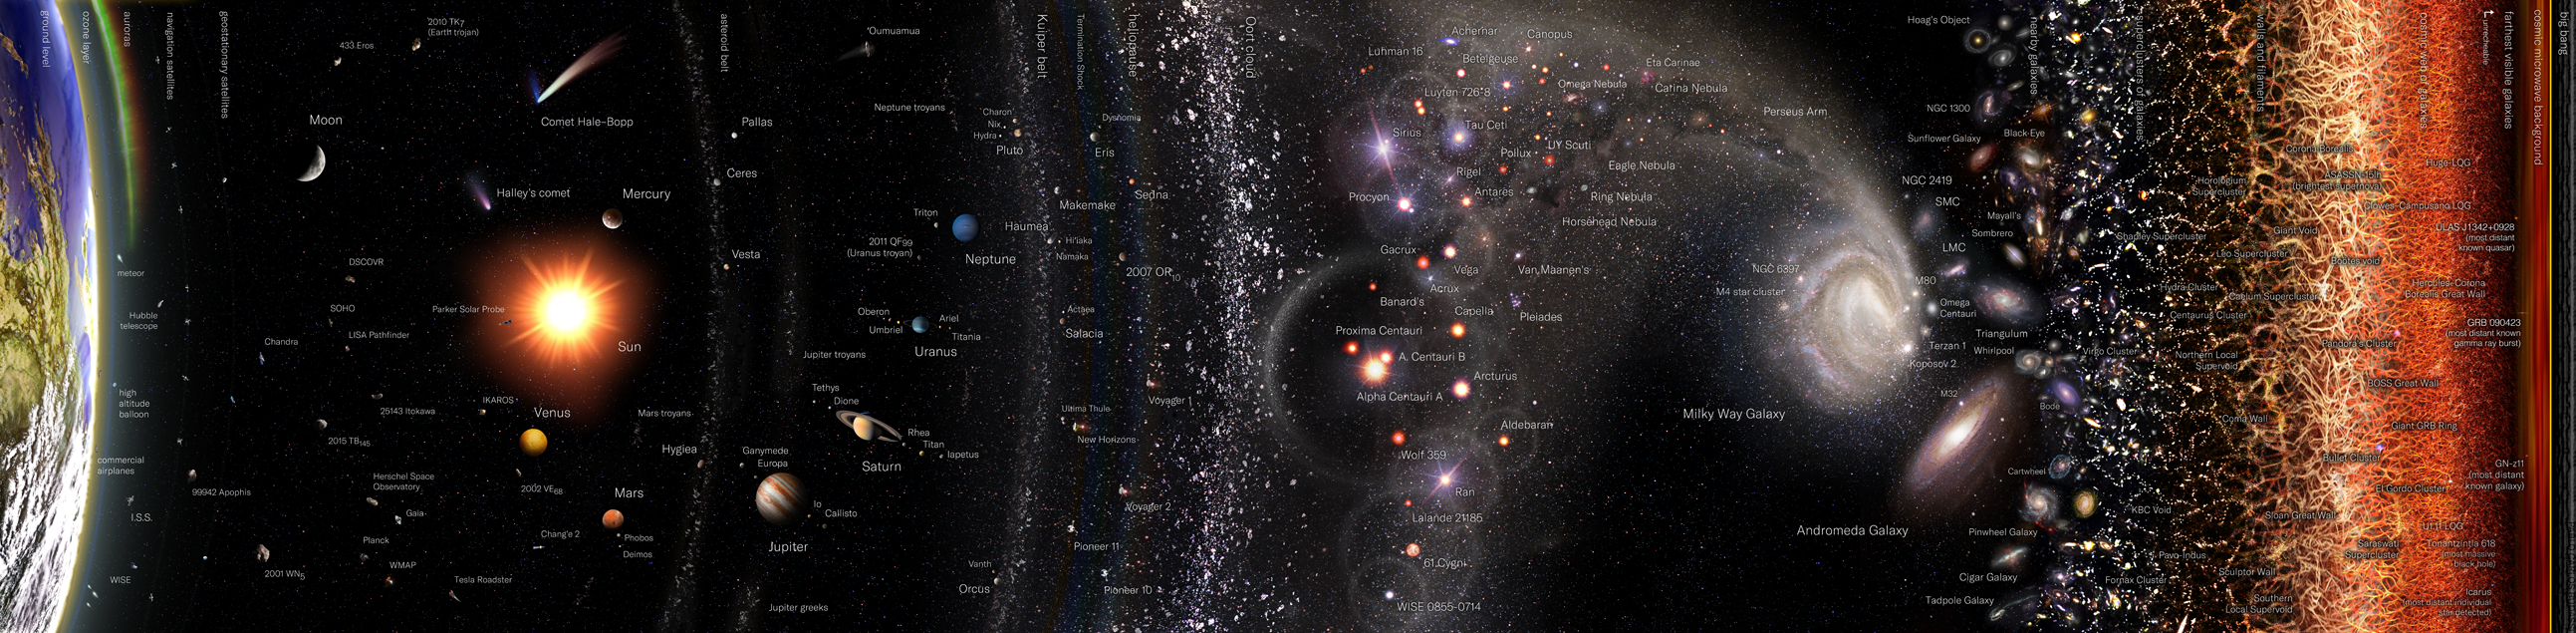
\includegraphics[width=\textwidth]{observable_universe.png}
  \caption{
    Artistic rendering of the observable universe, shown on a logarithmic scale from left to right based on proximity to Earth. Figure by Pablo Carlos Budassi.
  }
\end{figure}

In most (if not all) fields related to astrophysics research deals with \emph{plasma}, as it is by far the most abundant form of ordinary matter in the universe (we say ``ordinary'' here as we explicitly exclude exotic stuff such as dark matter and dark energy). A plasma can be simplified as an ionised gas, hence a significant part of it are charged particles which in turn implies that electromagnetic fields are of extreme importance. Depending on the amount of neutral particles present a plasma can either be fully ionised (no neutrals) or partially ionised (some neutrals). In this thesis we only consider a fully ionised plasma, which will be quite sufficient for (most of) our applications.

The tools used to study astrophysics vary greatly, and similar to the various disciplines depend on which objects are being studied. In the time of Newton and Galilei tools mostly consisted of early telescopes and basic mathematical methods. Over the years new theories have been developed, where Einstein's general relativity is probably the most notable in an astrophysical context, which came accompanied with numerous advances and physical insights. From an observational viewpoint we evolved from using basic, simple telescopes to (arrays of) huge ground and space based telescopes and observatories designed to probe the deepest reaches of our universe. Additionally, with the advent of the computer age a completely new set of tools became available: suddenly it was possible to numerically solve systems of equations that were previously unsolvable using analytical methods, and this in turn sparked a whole new branch of computational astrophysics. Large-scale numerical codes have been developed since then, which can exploit a huge number of computational resources in parallel using the most powerful supercomputers on the planet. This has opened a completely new door into the wonderful world of astrophysics, where it is now possible to numerically probe and visualise even the most exotic astrophysical objects at extreme resolutions.

The field of solar physics studies, as the name suggests, our sun. Even here research topics are widely spread out, ranging from the solar interior to features on the solar surface, to the entire solar atmosphere, the link between the solar wind and space weather, to name a few. In this thesis we will mainly focus on waves and instability aspects from a spectroscopic standpoint, which can be directly linked to interesting structures in the solar atmosphere, that is, parts of the solar corona and chromosphere. We will mainly rely on numerical approaches, supplemented with a strong mathematical foundation.


\section{The Sun in a nutshell}
Our sun, at a distance of approximately 150 million kilometres, is the closest star to Earth and is directly responsible for all life on this planet. Roughly five billion years ago a ``baby'' sun (or proto-star) formed as a contracting molecular cloud, slowly heating up in the process. Once the proto-star's core temperature became high enough nuclear fusion kicked in, converting hydrogen to helium. This signalled a delicate balance between inwards gravitational forces and the outwards push of energy in the form of luminosity, contraction ceased, and our sun entered its main sequence phase as a standard G-type main sequence star. Since then it has been happily burning hydrogen and turning it to helium in its core, and will continue to do so for roughly another 5 billion years. At that point all hydrogen in the core will be exhausted and the star will expand into a red giant, eventually turning into a white dwarf.

The sun is essentially a giant ball of plasma with various internal regions having different physical properties. We will not discuss the overall structure of the solar interior here, but focus only on the solar atmosphere. The sun does not have a strict ``surface'', in the sense that there is no abrupt border between the atmosphere and interior like we have here on Earth; it rather is defined as the part of the sun where photons can easily escape into space. This is marked by an optical depth of $\tau_\nu \approx 1$, which is a measure of how a given intensity is absorbed when it passes through a certain layer, in essence the transparency of this layer. The solar interior has an optical depth which is much larger than one, whereas the solar exterior has an optical depth much less than one, and can (for the most part) be considered to be optically thin. For an extensive discussion on the properties of the solar interior and exterior, see \citet{book_priest}.

Figure \ref{fig: solar_profile} shows a sketch of the solar atmosphere, which can be divided into three separate regions. While in reality the entire atmosphere is highly dynamic and varying in time, for all intents and purposes we can conveniently model it as three layers with different properties. The first one is called the \emph{photosphere}, which is a thin layer only a few 100 kms thick emitting most of the sun's visible light. It is pervaded with granulation of different sizes, owing their existence to convective cells originating from within the solar interior, implying that there is quite a lot of turbulence present throughout the entire solar photosphere.
\begin{figure}[t]
  \centering
  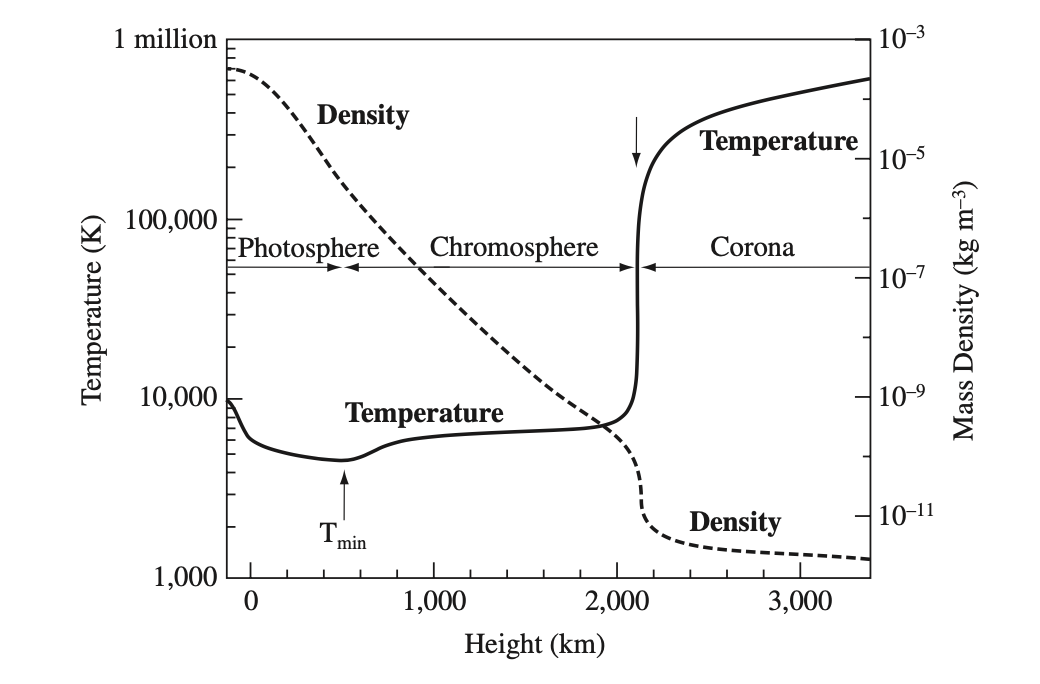
\includegraphics[width=\textwidth]{solar_profile.png}
  \caption{
    Schematic of the mean variation of the temperature and density in the solar atmosphere as a function of height.
    Figure taken from \citet{book_priest}.
  }
  \label{fig: solar_profile}
\end{figure}

The second layer is called the \emph{chromosphere}, which starts at the upper photosphere and has a fairly constant temperature with decreasing density for increasing distance from the surface. The chromosphere also contains the transition from $\beta > 1$ to $\beta < 1$, in which $\beta$ is given by
\begin{equation} \label{eq: plasma_beta}
  \beta = \frac{p_\text{gas}}{p_\text{magnetic}} = 2\mu_0 \frac{p_\text{gas}}{B^2}.
\end{equation}
Here $B$ denotes the magnetic field and $\mu_0$ the magnetic permeability in vacuum, equal to $4\pi$ in cgs units. The above quantity, called the \emph{plasma-$\beta$}, is defined as the ratio between gas pressure and magnetic pressure and is thus a measure of the relative importance of the magnetic field. For $\beta > 1$ the plasma forces dominate, which is for example the case in the solar photosphere. On the other hand, $\beta < 1$ indicates that the magnetic forces are dominant, which is the case for most of the solar corona and part of the solar chromosphere.

The chromosphere ends at the sudden rise in temperature and drop in density which is called the
\emph{transition region}. In this very narrow region of about 100 km the plasma jumps from approximately 20 000 K in the upper chromosphere to over a million K, which marks the start of the \emph{solar corona}, the third and final region in the schematic shown in Figure \ref{fig: solar_profile} and the outermost layer of the solar atmosphere. The entire corona is full of fascinating structures such as solar prominences and coronal loops, and at high altitudes the corona gives rise to the solar wind, continuously blowing plasma and particles into space.

\begin{figure}[t]
  \centering
  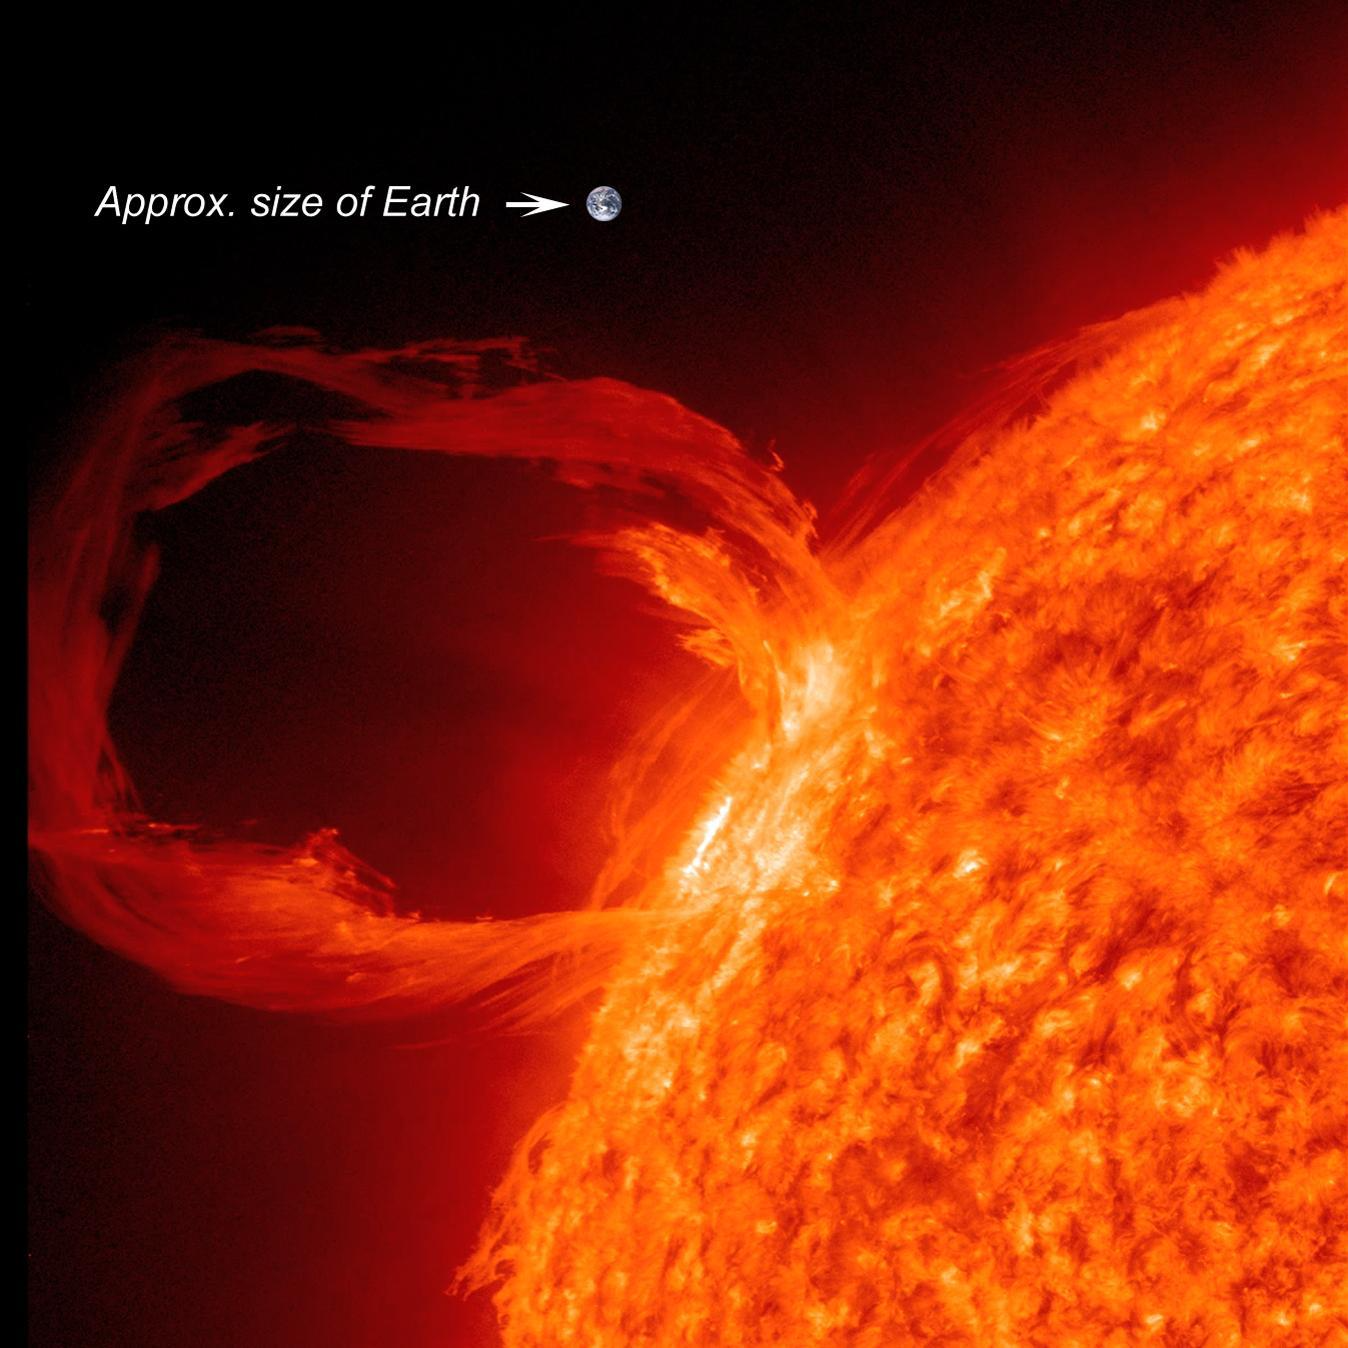
\includegraphics[width=0.6\textwidth]{solar_prominence.png}
  \caption{
    Eruptive prominence in He II at 304 {\AA} from 10 March 2010, the size of the Earth is indicated on the figure for scale. Figure from NASA/SDO/AIA.
  }
  \label{fig: solar_prominence}
\end{figure}

We will briefly discuss solar prominences in this introductory part, as they are highly relevant in the scope of Chapter \ref{ch: thermal instability}. In essence, solar prominences are large, cool, and dense structures suspended along magnetic field lines, that have their footpoints near the photosphere and extend thousands of kilometres outwards into the hot corona. They form most likely through the process of thermal instability (TI), where a runaway radiative cooling effect leads to increased energy losses through radiation, eventually leading to plasma motions that locally increase the density while energy losses drastically lower the temperature further. The resulting condensations are orders of magnitude denser and hotter than their surroundings and initial conditions, with their plasma suspended by magnetic fields high above the solar surface. This is the in-situ ``condensation'' approach to solar prominence formation, where plasma condenses in-place due to thermal instability and forms a flux rope. In the past few years variants of this process have been proposed.
The first one is an ``evaporation-condensation'' process, wherein chromospheric plasma is evaporated due to localised footpoint heating and thereby feeds material to the coronal volume, where it then condenses due to thermal instability. The steady supply of mass in this model overcomes the limitations of an in-situ TI approach, and it has been successfully employed to model solar prominences \citep{xia2016} and study the formation of coronal rain \citep{fang2013,moschou2015,xia2017}.

The second process is an injection-based model, where one can distinguish between two scenarios: ``levitation-condensation'' and ``reconnection-condensation''. The former is less dramatic than the latter, but both involve some sort of magnetic reconnection to eject plasma upwards into the solar corona instead of a steady supply through evaporation. This plasma eventually settles in already present topological dips in the field lines. The levitation mechanism mostly lifts cool, relatively static chromospheric material upwards, directly into the body of the flux rope \citep{kaneko2015,zhao2017,jenkins2021}. The reconnection mechanism on the other hand usually involves injecting material straight from the footpoints in a much more dynamic way \citep{kaneko2017}. In both scenarios the propelled material is heated to some degree due to the reconnection process, and eventually condenses through TI.
Finally, \citet{zhao2022} recently proposed a new scenario where a current sheet underneath the flux rope gives rise to magnetic islands (plasmoids), which in turn transport cool and dense chromospheric matter to the flux rope, eventually forming a prominence with coronal plasma continuously condensing through TI. Thermal instability obviously plays a critical role in all these scenarios, making a thorough understanding of TI as a whole of paramount importance.

If these giant structures become unstable they can burst outwards as an eruptive prominence. Figure \ref{fig: solar_prominence} shows such a large, eruptive prominence in He II at 304 \AA, from 10 March 2010; the Earth is superimposed for scale, making the enormous size of these structures apparent. It immediately becomes clear that waves and instabilities play a major role here. How, why and when do these structures become unstable? Can it be traced back to instabilities during their formation process? Or are there new instabilities that arise? If so, where do they come from? Furthermore, most prominences show intriguing fine structure, and it is at present still largely unknown where that originates from.

\section{The importance of instabilities}
The questions mentioned in the previous paragraph highlight the importance of wave and instability studies in all kinds of settings, not only limited to solar applications but highly relevant to a wide range of scientific disciplines. In hydrodynamics (fluids and gasses), one of the most well-known instabilities is the Kelvin-Helmholtz instability, originating from a velocity shear at the interface between two fluids (e.g. \citep{book_choudhuri}). This type of instability is commonly found in many laboratory, astrophysical and space plasmas, with some common examples being characteristic cloud formations here on Earth, ripples at the interface between solar prominences and the corona; and even near the Great Red Spot on Jupiter (see Figure \ref{fig: kh_instability}).

\begin{figure}[b]
  \centering
  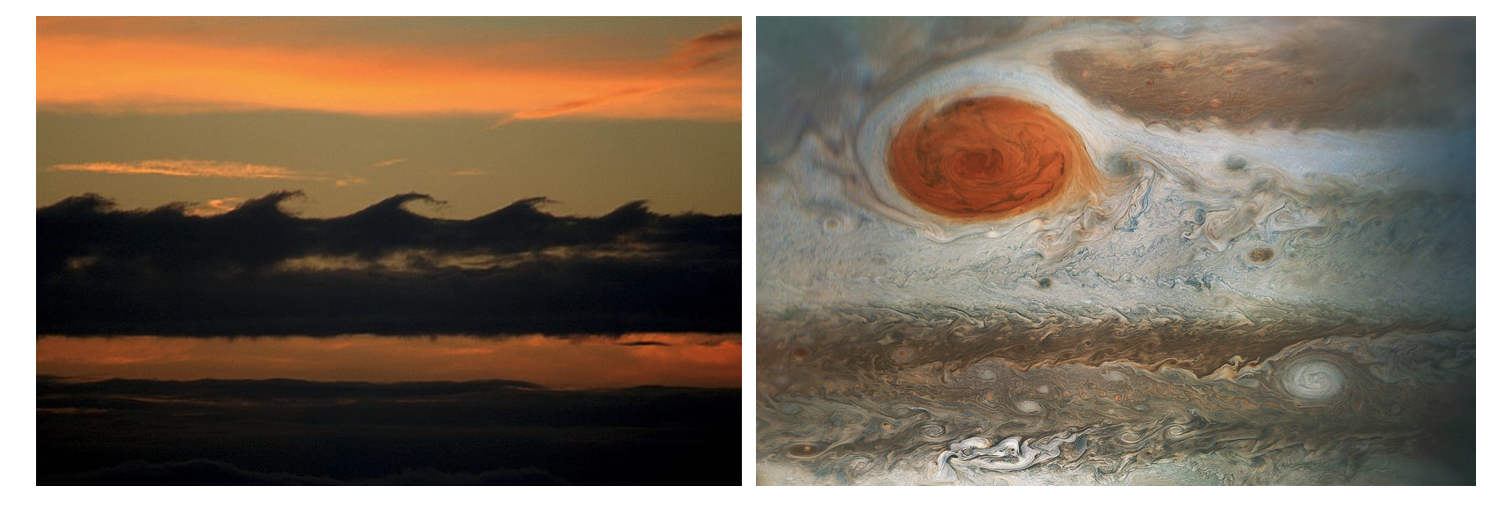
\includegraphics[width=\textwidth]{instabilities.png}
  \caption{
    Examples of Kelvin-Helmholtz instabilities in cloud formations (left) and near Jupiter's Great Red Spot (right), note the characteristic vortices for both cases. Left figure by Brocken Inaglory, right figure by NASA/JPL.
  }
  \label{fig: kh_instability}
\end{figure}

As mentioned earlier thermal instability lies at the basis of solar prominence formation, but is directly relevant to a broader astrophysical context as well. Thermal instabilities have been encountered in dense molecular clouds in the warm interstellar medium, where they can be responsible for high density filaments in star-forming regions; in galactic clusters and haloes; and even in thin discs' accretion onto stellar-mass black holes where they can cause a vertical collapse of the disk. Thermal instability can occur both in hydrodynamics as in magnetohydrodynamics (plasmas), where in case of the latter the addition of a magnetic field further complicates the picture; thereby not only affecting thermal instability but all other aforementioned instabilities as well.

Magnetic fields may give rise to an even richer collection of possible instabilities in a given system. One of the more dramatic changeovers in magnetohydrodynamics lies in the introduction of magneto-rotational routes to turbulence, at play in accretion disks around black holes or in protoplanetary disks around newly formed stars \citep{balbus1991}. Not only is this well-known magnetorotational instability (MRI) important here: recent work by \citet{goedbloed2022_sari} found that a new type of mode, the Super-Alfv\'enic Rotational instability (SARI), is of essential importance for instability studies of accretion disks. The relevance of waves and instabilities does not limit itself to astrophysical settings, but also holds for magnetised applications accessible to laboratory experiments. This even extends to controlled nuclear fusion research, where MHD spectroscopy -- that is, classifying the various linear waves and (in)stabilities of a system -- is already the pre-eminent tool used to delimit operational windows: instabilities can strongly disrupt a given system and are to be avoided at all costs.


\section{General outline}
Due to the huge applicability and interdisciplinary importance of linear stability studies the topic is vast, and numerous investigations have been done over the past decades. However, research in this field usually takes one of two main approaches: either direct numerical simulations are performed in two or three dimensions, which is quite resource intensive and time-consuming; or a theoretical approach is considered in which the required dispersion relation makes it necessary to use (greatly) simplifying assumptions due to the complexity of the problem at hand. In this thesis we plan to take a different approach to waves and instabilities, and tackle (thermal) instabilities from a spectroscopic viewpoint. We therefore take a stepwise approach and formulate the following:
\begin{enumerate}
  \item[i)] How do linear waves trigger or evolve into nonlinear thermal instability for local coronal volumes?
  \item[ii)] In the nonlinear regime, is there a link between thermal instability and fine structure?
  \item[iii)] Moving away from simplified setups, what does the spectrum of a realistic solar atmosphere look like?
  \item[iv)] What role do thermal instabilities have in this?
\end{enumerate}

These can be regarded as the ``science questions'' we want to look at in this thesis, with point iii) and iv)  being quite challenging. In order to lay a solid foundation we dedicate Chapter \ref{ch: spectroscopy} to a thorough introduction to MHD spectroscopy, paying special attention to the non-adiabatic terms.

Chapter \ref{ch: thermal instability} builds further upon this, where a combined numerical and theoretical approach in a simplified uniform setup allows us to derive eigenfunctions for slow MHD modes, which can then be excited in a numerical domain with solar coronal conditions. We can make sure that the thermal mode is unstable, and we can take a close-up look at the dynamical and temporal evolution of the system as a whole. This gives us a first answer to points i) and ii).

In order to look at point iii) we need to move away from ``simple'' setups, which implies that problems can no longer be treated analytically. Therefore, in Chapter \ref{ch: legolas} we lay the foundations for the development of a brand new numerical tool, {\legolas}, which will allow us to do MHD spectroscopy of one-dimensional equilibria with a plethora of physical effects, for a general configuration that achieves force and thermodynamic balance. We introduce the weak Galerkin form of the linearised and Fourier-analysed MHD equations, which in turn transforms the set of equations in a generalised eigenvalue problem that can be solved using various linear algebra routines. This results in a complete set of eigenvalues and eigenfunctions for a given state, allowing us to probe the various waves and (in)stabilities at high resolutions.

In Chapter \ref{ch: legolas_applications} we test {\legolas} against a whole range of well-established results: from $p$ and $g$ modes in magnetised, stratified atmospheres; to modes relevant for coronal loop seismology; thermal instabilities; and instability studies of astrophysical jet flows. We show an excellent correspondence with known results, thereby thoroughly testing the implementation of our new code.

Finally, with {\legolas} we are in a place to answer points iii) and iv), and hence look at a realistic, empirical solar atmosphere model in Chapter \ref{ch: solar_atmosphere} and calculate the full eigenvalue spectrum for different chromospheric and coronal regions. This yields new insights in the behaviour of the thermal and slow continua, as well as in the thermal stability of these kinds of configurations.




\cleardoublepage

\chapter{MHD waves and spectroscopy} \label{ch: spectroscopy}

\graphicspath{{02-MHD_spectroscopy/figures/}}

\begin{chapterquote}[Eugene Parker][][]
  I'm proud of the fact that I thought of the solar wind. It was an exercise in pursuing curiosity, which is the main motivation for studying physics from a personal standpoint.
\end{chapterquote}

This Chapter provides an overview of the main principles of MHD spectroscopy and how one usually goes about detailing all waves and instabilities of a given physical equilibrium. Doing so can either be straightforward and yield relatively simple results, or can be quite complicated to the point where solutions show so many detailed features and intricacies that it is difficult to see the forest for the trees. Due to this inherent range in complexity of the problem at hand we adopt a step-by-step approach. Focusing on uniform equilibria at first, we look into simple waves and instabilities present in these plasmas and pay special attention to how the spectrum changes when more physics are included. In this Chapter we will limit ourselves to non-adiabatic effects: heating, cooling and thermal conduction.

This will already provide us with a myriad of information regarding the underlying physics at play in simple configurations, though eventually we want to move on to more realistic equilibria by introducing non-uniformity in the background. At that point we will hit the limit of what can be solved analytically, and the discussion in this chapter will shift to a more qualitative approach. This will get picked up again in later Chapters, where we will go more in-depth on how to tackle this particular problem and take a closer look at all the interesting features that emerge when solving it.

\section{Introduction}
Magnetohydrodynamics (MHD) is the cornerstone of plasma physics, and in an ideal setting describes the behaviour of a perfectly conducting fluid when it interacts with a magnetic field. In essence, MHD combines the Euler equations of gas dynamics with Maxwell's equations to describe the evolution of a magnetised plasma on macroscopic scales. This is the direct opposite of \emph{kinetic theory} (basically the other cornerstone of plasma physics), which describes plasmas using a collection of microscopic particles.

We will not go in-depth as to which theory is better suited for one particular problem or under which conditions they are valid approximations. Generally speaking if one is investigating very small spatial or temporal scales, or is interested in the motions of individual particles or particle species then kinetic theory is the best option. On the other hand, for ``larger'' applications in which one assumes that the collisions between individual particles happen so frequently that the plasma can be treated as a single continuous fluid then MHD is the way to go. Throughout this thesis we will assume that the latter is always the case, and we stick with the MHD representation.

One beautiful feature of the MHD equations is that they are \emph{scale-independent}. The equations themselves are made dimensionless by choosing (generally speaking) reference values for the typical length scale, magnetic field strength and plasma density. Depending on the problem at hand different reference values can be chosen to describe the situation, which in turn implies that MHD can describe plasmas in astrophysical settings (accretion disks, jets around black holes, stellar atmospheres, etc.) as well as laboratory settings, all using the same set of equations!
\emph{Throughout this thesis we will always work with normalised quantities, unless explicitly specified otherwise.}


\section{Magnetohydrodynamics}
\subsection{The ``simple'' MHD equations}
We first start with ``simple'' MHD, that is, constraining ourselves to the ideal equations. The word ``simple'' is placed between quotation marks here, as the ideal MHD equations are rather straightforward compared to their counterparts in which various non-ideal physical effects have been added. However, from a mathematical point of view even these relatively simple equations still describe a system of eight hyperbolic partial differential equations, which are \emph{not at all} easy to solve. For that we have to rely on numerical methods and dedicated codes, which are whole topics in itself. As the explicit derivation of these equations is standard material in any textbook on plasma physics, my favourite being \citet{book_MHD}, we will simply give their final (ideal) form below.

\begin{gather}
  \frac{\partial \rho}{\partial t} = -\nabla \cdot (\rho \bv), \label{eq: ideal_continuity} \\
  \rho \frac{\partial \bv}{\partial t} =
    -\nabla p
    - \rho \bv \cdot \nabla \bv
    + (\nabla \times \bb) \times \bb, \label{eq: ideal_momentum}\\
  \rho \frac{\partial T}{\partial t} =
    -\rho \bv \cdot \nabla T
    -\gmone p \nabla \cdot \bv, \label{eq: ideal_energy} \\
  \frac{\partial \bb}{\partial t} = \nabla \times (\bv \times \bb), \label{eq: ideal_induction}
\end{gather}
consisting of the continuity equation \eqref{eq: ideal_continuity}, momentum equation \eqref{eq: ideal_momentum}, energy equation \eqref{eq: ideal_energy} and induction equation \eqref{eq: ideal_induction}. The quantities $\rho$, $\bv$, $p$, $\bb$ and $T$ denote the plasma density, velocity field, pressure, magnetic field and temperature, respectively. The ratio of specific heats is denoted by $\gamma$ and is taken to be equal to $5/3$. The system is constrained by the divergence-free condition on the magnetic field $\nabla \cdot \bb = 0$, ensuring no magnetic monopoles, and the (normalised) ideal gas law $p = \rho T$. In three dimensions this results in eight equations and eight unknown variables $(\rho, \bv, T, \bb)$.

\subsection{The non-adiabatic MHD equations}
In the previous Subsection we discussed ideal, adiabatic MHD, meaning that no energy is gained or lost by the system and any change in internal energy is due to work. One can now wonder how everything is affected when this is not the case, that is, energy is gained by the system (though heating, for example), at the same time lost through radiation and on top of that there is internal energy transfer through the process of thermal conduction. When these effects are included in our representation we are talking about the \emph{non-adiabatic MHD equations}.

Mathematically the heating and cooling terms are represented by a quantity known as the \emph{heat-loss function} $\HLF$, defined as energy losses minus energy gains
\begin{equation} \label{eq: cooling_simple}
  \HLF(\rho, T) = \rho \HLFcool - \HLFheat,
\end{equation}
which is generally dependent on density and temperature. In this representation the heating function $\HLFheat$ is assumed to be constant in time. The quantity $\HLFcool$ is a tabulated set of temperature-dependent values resulting from detailed atomic and molecular calculations, to which we hereafter refer to as the ``cooling curve''.

For magnetised plasmas heat transfer through thermal conduction has a preferred direction, in this case the effect is a few orders of magnitude stronger along the magnetic field lines than across them. To model this anisotropy we make use of the thermal conductivity tensor $\bkappa$, given by
\begin{equation} \label{eq: conduction}
  \bkappa = \kappapara\unit{B}\unit{B} + \kappaperp\left(\idmat - \unit{B}\unit{B}\right).
\end{equation}
Here $\idmat$ is the identity matrix and $\unit{B} = \bb/B$ is a unit vector along the magnetic field. The quantities $\kappapara$ and $\kappaperp$ denote the thermal conduction coefficients parallel and perpendicular to the magnetic field lines and are taken equal to the Spitzer conductivity \citep{book_priest}
\begin{equation} \label{eq: thermal_coeffs}
  \begin{gathered}
    \kappapara \approx 8 \times 10^{-7} T^{5/2}, \\
    \kappaperp \approx 4 \times 10^{-10} n^2 B^{-2} T^{-3} \kappapara,
  \end{gathered}
\end{equation}
both in units of erg cm$^{-1}$ s$^{-1}$ K$^{-1}$. Here $n$ denotes the number density, given by $n = \rho \massp$ with $\massp$ the proton mass.

Both the cooling and conduction terms are then added to the appropriate MHD equation, such that the adiabatic energy equation \eqref{eq: ideal_energy} transforms into the non-adiabatic energy equation
\begin{equation} \label{eq: nonad_energy}
  \rho \frac{\partial T}{\partial t} =
    -\rho \bv \cdot \nabla T
    -\gmone p \nabla \cdot \bv
    -\gmone \rho \HLF
    +\gmone \nabla \cdot \left(\bkappa \cdot \nabla T\right).
\end{equation}


Generally speaking, when numerically solving the system of MHD equations one relies on a similar set of steps no matter the approach taken. First a geometry is chosen depending on the problem at hand: a Cartesian (rectangular) box is convenient when describing for example parts of the solar atmosphere, while cylindrical geometries are more useful to describe problems like expanding flux tubes or jets. Next an initial state is chosen at time $t = 0$ fitting the problem, which essentially boils down to choosing initial prescriptions for $(\rho, \bv, T, \bb)$:
\begin{equation}
  \begin{gathered}
    \rho_\text{i}(\bx) \equiv \rho(\bx, t=0), \qquad T_\text{i}(\bx) \equiv T(\bx, t=0), \\
    \bv_\text{i}(\bx) \equiv \bv(\bx, t=0), \qquad \bb_\text{i}(\bx) \equiv \bb(\bx, t=0),
  \end{gathered}
\end{equation}
all depending on the position vector $\bx$. Since we are dealing with partial differential equations, appropriate boundary conditions must be chosen on all sides of the domain under consideration. Once the initial setup is chosen, the set of equations \eqref{eq: ideal_continuity}-\eqref{eq: ideal_induction} is written in conservative form and the domain is discretised using one particular resolution (or more in cases of mesh refinement). Then the iterative process can start: once one's favourite numerical scheme is chosen all fluxes through every cell in the domain are calculated and the system is advanced in time. These two steps are repeated until the simulation ends and/or the system reaches a stationary state.

Naturally, it is clear that higher resolutions result in much finer cells, which in turn may reveal more features. The major downside here is that more cells require more calculations, and in three dimensions the number of calculations required to advance the simulation even a single timestep scales with the third power in resolution. This requirement can be somewhat mitigated by using mesh refinement, i.e. focusing high resolutions on regions of interest in the domain while keeping the other regions at lower resolutions. In most, if not all, of these cases however one usually has to resort to supercomputers in order to run these simulation at a decent resolution.



\section{Introduction to MHD spectroscopy}
The main question that spectroscopy tries to answer is ``\emph{How do you know, without explicitly solving the entire set of equations, whether a given dynamical system is stable or not}''? Figure \ref{fig: stability} gives an illustration of the theoretical approach to linear stability analysis. Consider a solid ball at rest at an initial time $t = 0$ on some sort of hill in a gravitational field. If no forces are acting on this ball, then it will remain in this initial position indefinitely. When a small perturbation is applied, i.e. moving the ball slightly away from its equilibrium position, a number of things may happen depending on the shape of the surface the ball is resting on.

\begin{figure}[b]
  \centering
  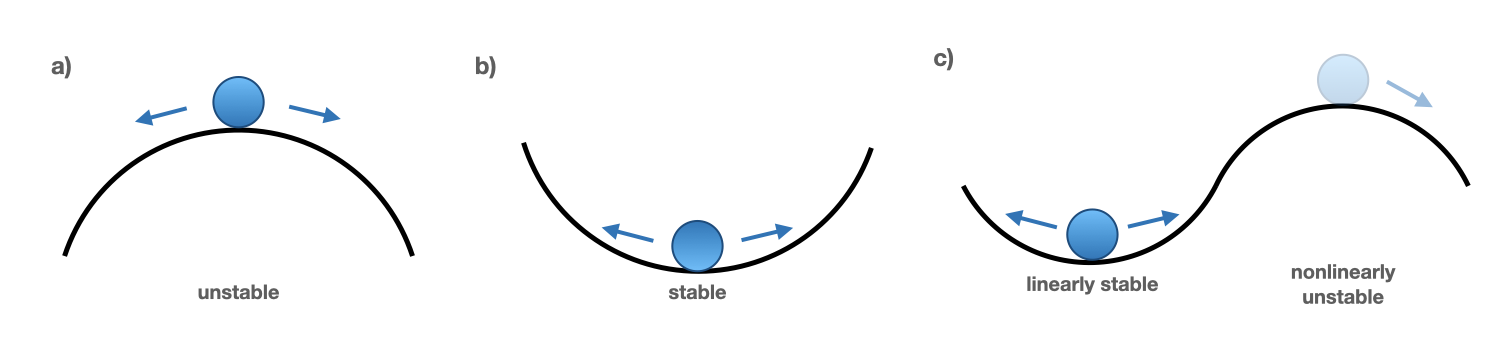
\includegraphics[width=\textwidth]{stability.png}
  \caption{Panel \textbf{a}: Unstable system; Panel \textbf{b}: Stable system; Panel \textbf{c}: Linearly stable, nonlinearly unstable system.}
  \label{fig: stability}
\end{figure}

In Panel a the ball is clearly laying on top of a hill, and any shift in initial position will cause it to roll downwards under the influence of gravity. This is called an \emph{unstable} configuration: no matter how small the perturbation is, there is no way to restore the initial equilibrium after the perturbation is applied.
In Panel b we have the exact opposite: shift the ball away from its initial location and it will simply roll downwards again, oscillating back and forth around its position at $t = 0$. Assuming there is some friction present between the ball and the surface, it will eventually come to a standstill again after some time $t$ in the same position as it started in. This is called a \emph{stable} configuration, and in this case even relatively large perturbations will have no major effect on the system as a whole.

Panel c on the other hand is much more interesting. Following the same train of thought as for the other two panels, \emph{small} perturbations will return the ball to its equilibrium position. However, if the perturbation is large enough the ball may gain enough energy to reach the peak on the right, roll over, and it will never be able to reach its equilibrium position again. This is called \emph{nonlinear instability}: a system that is stable for small perturbations, but may become unstable for larger perturbations.

Thermal instabilities (TI), the main topic of the next Chapter, can be classified in this latter category. These instabilities are called \emph{thermal} since they originate from the non-adiabatic terms in the energy equation \eqref{eq: nonad_energy}, in particular the radiative cooling terms. A system that is loosing energy through radiation and gaining energy through background heating may be stable to small temperature fluctuations, where a restoring force such as magnetic tension/pressure or thermal conduction (which smoothens out variations in temperatures if they are small enough) can counteract the instability and bring the system back in thermal equilibrium. This is the linearly stable regime on the left side of Panel c, Figure \ref{fig: stability}. If the fluctuations are large enough to overcome the restoring forces analogous to the right side of Panel c then a thermal runaway reaction occurs (instability), drastically lowering the temperature. A thorough discussion on the nature of thermal instabilities will be given in the next Chapter.

\subsection{Linearisation of the system}
Now that we have given a simplified example as to get a feel for linear stability analysis, we can start tackling the problem mathematically. Starting with the simplest case, that of a homogeneous background, will already prove quite instructive and will pave the path for more complex treatments later on.

Stability analysis of the MHD equations is done through a process called \emph{linearisation}, which essentially means splitting our equations in an equilibrium part and a dynamical part, where we assume that the latter is a small perturbation (subscript $1$) with respect to the equilibrium state (subscript $0$), such that a quantity $f$ can be written as
\begin{equation} \label{eq: linear_split}
  f(\bx, t) = f_0(\bx, t) + f_1(\bx, t).
\end{equation}
We start by defining the background equilibrium and we hence assume that the dynamics of the system take place around this state. Since we want to start as simple as possible the first assumption we can make is to have a static background, meaning there are no flow effects: $\bv_0 = 0$. The background is also assumed to be constant over time as it is in equilibrium, such that the temporal derivatives evaluate to zero. Furthermore, as mentioned earlier, we first look at a homogeneous background such that it is independent of position and the spatial derivatives become zero as well. The space-time dependence then only enters in the dynamical (perturbed) part of our assumption \eqref{eq: linear_split}. Mathematically this can be written as
\begin{equation} \label{eq: linear_homogeneous}
  \begin{gathered}
    \rho(\bx, t) = \rho_0 + \rho_1(\bx, t), \\
    \bv(\bx, t) = \bv_1(\bx, t), \\
    T(\bx, t) = T_0 + T_1(\bx, t), \\
    \bb(\bx, t) = \bb_0 + \bb_1(\bx, t).
  \end{gathered}
\end{equation}
The next step is plugging these expressions into the system of non-adiabatic MHD equations, and since we are interested in \emph{linear} perturbations we can ignore all higher-order terms $\mathcal{O}(f_1^2(\bx, t))$. Because of our assumptions in \eqref{eq: linear_homogeneous} the divergence-free condition $\nabla \cdot \bb_0 = 0$ is automatically satisfied. This is not necessarily the case for $\bb_1$ though, so we rewrite the perturbed magnetic field in terms of a magnetic vector potential using $\bb_1 = \nabla \times \ba_1$ such that $\nabla \cdot \bb_1 = \nabla \cdot \left(\nabla \times \ba_1\right) = 0$ is naturally satisfied as the divergence of a curl is always zero by definition.

When the non-adiabatic energy equation \eqref{eq: nonad_energy} is linearised this will contain a term $\rho_1\HLF_0$. Because we linearise around an equilibrium state, we require this state to be in \emph{thermal equilibrium}, implying that all energy gained through heating must be balanced by radiative cooling, resulting in a net difference of zero, hence $\HLF_0$ must be zero. As the heating is assumed to be constant this can be written as
\begin{equation}
  \HLF_0 = \rho_0\Lambda(T_0) - \HLFheat_0 = 0,
\end{equation}
such that the constant heating contribution $\HLFheat_0$ equals the radiative losses $\rho_0\Lambda(T_0)$ at $t = 0$, and the term with $\HLF_0$ drops out of the equations.

The \emph{linearised MHD equations} then read
\begin{gather}
  \frac{\partial \rho_1}{\partial t} = -\rho_0 \nabla \cdot \bv_1, \label{eq: linearised_rho1_homo}\\
  \rho_0 \frac{\partial \bv_1}{\partial t} =
    -\nabla\left(\rho_1 T_0 + \rho_0 T_1\right)
    +\left(\nabla \times \bb_0\right) \times \left(\nabla \times \ba_1\right) \nonumber \\
    +\left[\nabla \times \left(\nabla \times \ba_1\right)\right] \times \bb_0, \\
  \rho_0\frac{\partial T_1}{\partial t} =
    -\rho_0\bv_1 \cdot \nabla T_0
    -\gmone \rho_0 T_0 \nabla \cdot \bv_1
    -\gmone \rho_0 \left(\dHLFT T_1 + \dHLFrho \rho_1\right) \nonumber \\
    +\gmone \nabla \cdot \left(\bkappa_0 \cdot \nabla T_1\right)
    +\gmone \nabla \cdot \left(\bkappa_1 \cdot \nabla T_0\right), \\
  \frac{\partial \ba_1}{\partial t} = \bv_1 \times \bb_0, \label{eq: linearised_A1_homo}
\end{gather}
where the background dimensionless pressure is rewritten as $\rho_0 T_0$ and the perturbed pressure contribution $p_1$ has been replaced by $\rho_0 T_1 + \rho_1 T_0$ following the linearised ideal gas law. The quantities $\dHLFT$ and $\dHLFrho$ denote the temperature and density derivatives of the heat-loss function, respectively, which can be written as
\begin{equation} \label{eq: dHLF_homogeneous}
  \begin{gathered}
    \dHLFrho = \left.\frac{\partial \HLF}{\partial \rho}\right|_\text{T} = \Lambda(T_0), \\
    \dHLFT = \left.\frac{\partial \HLF}{\partial T}\right|_\rho =
      \rho_0 \left.\frac{d\Lambda(T)}{dT}\right|_{\text{T}_0},
  \end{gathered}
\end{equation}
which both have to be evaluated in the equilibrium quantities $\rho_0$ and $T_0$.

This set of linearised equations is still a system of partial differential equations. However, since the homogeneous equilibrium quantities $(\rho_0, \bv_0, T_0, \bb_0)$ do not depend on time we can consider plane-wave perturbations of the form
\begin{equation} \label{eq: plane_wave_homogeneous}
  f_1(\bx, t) = \tilde{f_1}\exp\Bigl(i\bk \cdot \bx - \icomplex\omega t\Bigr),
\end{equation}
where $\bx = (x, y, z)$ is the (Cartesian) position vector, $\omega$ a complex frequency, $\bk = (k_x, k_y, k_z)$ the wave vector and $\tilde{f_1}$ a (complex) constant denoting the amplitude of the plane wave. We are essentially doing a Fourier analysis in three ``ignorable'' dimensions. The wonderful consequence of doing this is that it transforms the temporal and spatial derivatives of the perturbed variables $f_1(\bx, t)$ into
\begin{equation}
  \frac{\partial}{\partial t} \rightarrow -\icomplex\omega, \qquad\qquad
  \nabla \rightarrow i\bk,
\end{equation}
which reduces the system of partial differential equations to a system of \emph{algebraic} equations given by
\begin{gather}
  \omega \rho_1 = \rho_0 \bk \cdot \bv_1, \label{eq: homo_continuity_algebraic}\\
  \rho_0\omega \bv_1 = T_0 \bk \rho_1 + \rho_0\bk T_1 - \icomplex[\bk \times (\bk \times \ba_1)]\times\bb_0, \\
  \rho_0\omega T_1 =
    \gmone \rho_0T_0 \bk \cdot \bv_1
    - \icomplex\gmone\rho_0\left(\dHLFT T_1 + \dHLFrho \rho_1\right) \nonumber \\
    - \icomplex\gmone \left(\kappapara \kpara^2 + \kappaperp\kperp^2\right)T_1, \\
  \omega \ba_1 = \icomplex\bv_1 \times \bb_0, \label{eq: homo_induction_algebraic}
\end{gather}
with $\kpara$ and $\kperp$ denoting the wave vector components parallel and perpendicular to the background magnetic field $\bb_0$, respectively. As confusion is not possible the tilde notation used in Equation \eqref{eq: plane_wave_homogeneous} has been omitted.

\subsection{Eigenvalues and stability}
The eight equations given in \eqref{eq: homo_continuity_algebraic}-\eqref{eq: homo_induction_algebraic} form a complete eigenvalue problem, with the eigenvectors containing the variables $\rho_1, \bv_1, T_1$ and $\ba_1$. This can be reduced to a standard complex eigenvalue problem of the form $\amat\statevec = \omega\statevec$, with general wave vectors $\bk = (k_x, k_y, k_z)$ and magnetic field vectors $\bb_0 = (B_{0x}, B_{0y}, B_{0z})$. The state vector $\statevec$ containing the unknown variables is then given by
\begin{equation}
  \statevec = \begin{pmatrix}
    \rho_1 & v_{1x} & v_{1y} & v_{1z} & T_1 & A_{1x} & A_{1y} & A_{1z}
  \end{pmatrix}^T.
\end{equation}
Due to the homogeneous background that was imposed the elements of the matrix $\amat$ are constants, and the eigenfrequency $\omega$ of each respective mode can be obtained by directly solving for the eigenvalues of the corresponding $\amat$-matrix. Generally speaking the eigenvalues are complex, hence every eigenvalue can be written as
\begin{equation}
  \omega \equiv \omega_\text{R} + \icomplex\omega_\text{I},
\end{equation}
where $\omega_\text{R}$ and $\omega_\text{I}$ denote the real and imaginary parts, respectively. Looking back at our plane-wave solutions in Equation \eqref{eq: plane_wave_homogeneous} this implies that the temporal behaviour of all waves scales as
\begin{equation}
  \sim \exp(\omega_\text{I} t)\exp(-\icomplex\omega_\text{R} t).
\end{equation}
From this the physical role of both components becomes clear: for purely real eigenvalues ($\omega_\text{I} = 0$) wave modes will propagate in the direction of $\bk$ and oscillate with a frequency $\omega_\text{R}$, these are stable waves and their amplitude will remain constant over time. The sign of $\omega_\text{R}$ represents forwards ($+$) or backwards ($-$) propagating modes with respect to the direction of $\bx$. For non-zero $\omega_\text{I}$ however one can distinguish between four scenarios:
\begin{enumerate}
  \item $\omega_\text{R} = 0$ and $\omega_\text{I} > 0$: \emph{unstable modes}. These are imaginary eigenvalues and represent pure instabilities. In this case, if the background is perturbed this will not result in propagating waves but in an exponential increase in amplitude.
  \item $\omega_\text{R} = 0$ and $\omega_\text{I} < 0$: \emph{damped modes}. These are also imaginary eigenvalues but the opposite of the previous case: amplitudes will decay exponentially over time.
  \item $\omega_\text{R} \neq 0$ and $\omega_\text{I} > 0$: \emph{overstable modes}. These eigenvalues are genuinely complex, with nonzero real and imaginary parts. This represents propagating waves which are unstable due to excessive feedback in the system, resulting in an increase in amplitude over time.
  \item$\omega_\text{R} \neq 0$ and $\omega_\text{I} < 0$: \emph{overdamped modes}. The opposite of the previous case, with again eigenvalues that are genuinely complex. These eigenvalues represent propagating waves with decreasing amplitude, eventually dying out such that the system returns to its equilibrium state.
\end{enumerate}

\begin{figure}[b]
  \centering
  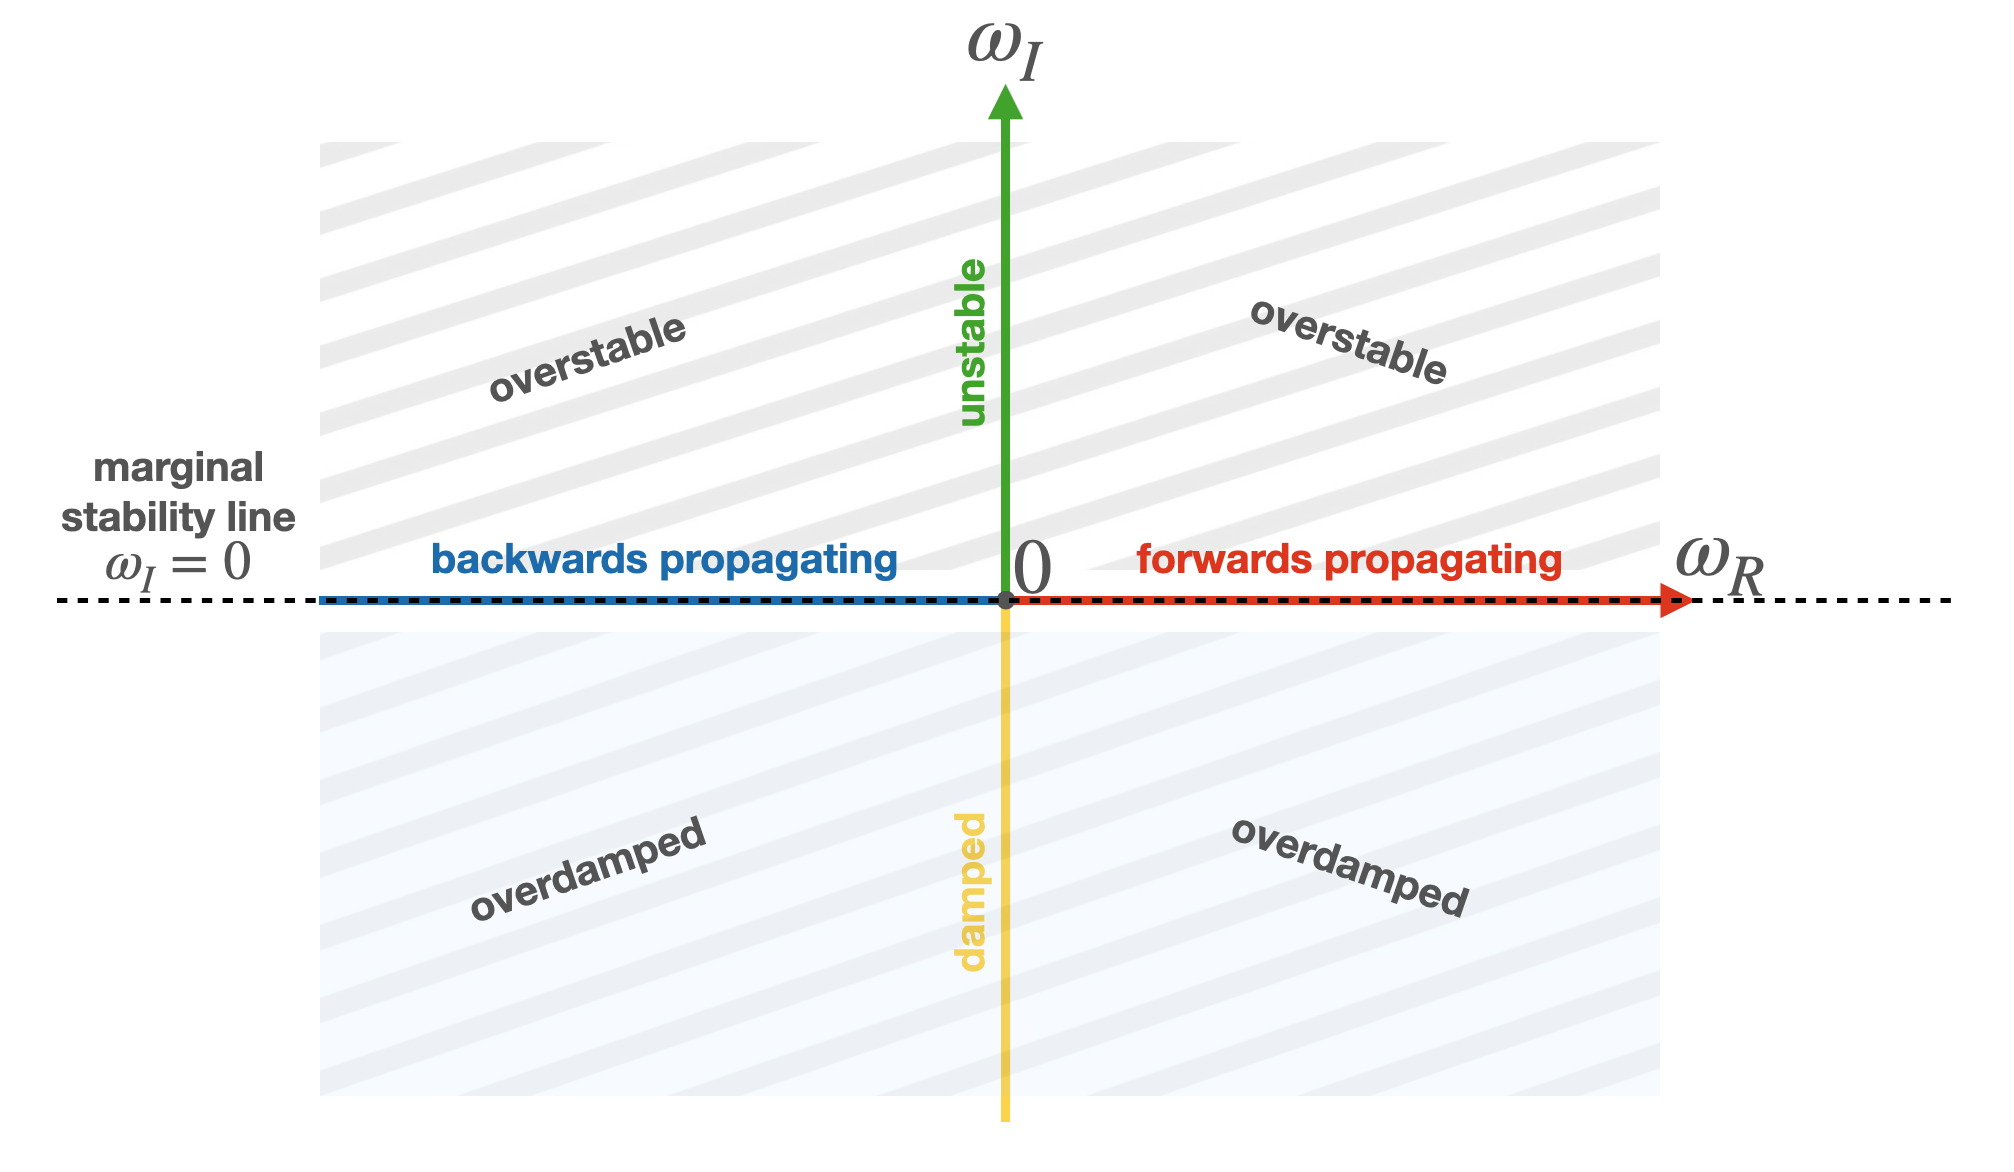
\includegraphics[width=0.9\textwidth]{spectral_plane.png}
  \caption{Graphical representation of various (in)stability regions and their terminology.}
  \label{fig: spectral_plane}
\end{figure}

Figure \ref{fig: spectral_plane} shows a graphical representation of all different cases, where all regions have been annotated in a $\omega_\text{R} - \omega_\text{I}$ 2D-plane. A complex plane like this is called a \emph{spectrum}, and we will use similar representations throughout this thesis to visualise eigenvalues. Additionally, in the remainder of this thesis we will not distinguish between damped and overdamped modes, both will simply be referred to as ``damped''.


\subsection{The ideal MHD spectrum}
When solving the eigenvalue system to obtain all eigenvalues some care must be taken, as will become clear in what follows. Since we are dealing with an $8 \times 8$ matrix one would immediately expect that we have eight eigenvalues, and thus eight ``waves'' in our system. In our earlier representation we have chosen a general wave vector and magnetic field vector, but we can always rotate our reference system to choose $\bb_0 = (0, 0, B_0)$ along the $z$-axis and $\bk = (k_\perp, 0, k_\parallel)$ in the $x-z$ plane without loosing generality. For the moment we focus on the ideal spectrum, omitting all non-adiabatic effects in the energy equation, such that the $\amat$-matrix in the ideal eigenvalue problem becomes
\begin{equation} \label{eq: ideal_matrix}
  \resizebox{0.89\hsize}{!}{$
    \begin{pmatrix}
      0 & \kperp \rho_0 & 0 & \kpara \rho_0 & 0 & 0 & 0 & 0 \\
      \dfrac{T_0}{\rho_0}\kperp & 0 & 0 & 0 & \kperp & 0 & \dfrac{\icomplex B_0}{\rho_0}k_0^2 & 0 \\
      0 & 0 & 0 & 0 & 0 & -\dfrac{\icomplex B_0}{\rho_0}\kpara^2 & 0 & \dfrac{\icomplex B_0}{\rho_0}\kpara \kperp \\
      \dfrac{T_0}{\rho_0}\kpara & 0 & 0 & 0 & \kpara & 0 & 0 & 0 \\
      0 & \gmone T_0 \kperp & 0 & \gmone T_0 \kpara & 0 & 0 & 0 & 0 \\
      0 & 0 & \icomplex B_0 & 0 & 0 & 0 & 0 & 0 \\
      0 & -\icomplex B_0 & 0 & 0 & 0 & 0 & 0 & 0 \\
      0 & 0 & 0 & 0 & 0 & 0 & 0 & 0
    \end{pmatrix},
  $}
\end{equation}
with $k_0^2 = \kpara^2 + \kperp^2$. This introduces a zero row in the matrix, which essentially originates from the $\nabla \cdot \bb = 0$ constraint which is naturally satisfied in our representation. If we would have kept the magnetic field as-is instead of transforming to a vector potential, this zero row would not have been present. However, in that case we still would have to take the divergence-free constraint into account by eliminating one of the magnetic field variables to obtain a $7 \times 7$ matrix representation. All of this implies that instead of eight solutions to the eigenvalue problem we actually have \emph{seven} solutions and one \emph{spurious} $\omega = 0$ eigenvalue.

In ideal MHD the $\amat$-matrix is Hermitian (i.e. its own conjugate transpose; the matrix operator is self-adjoint), which has interesting consequences for the solutions. From a spectral viewpoint this implies that all eigenvalues either lie \emph{on} the real or imaginary axis, and that there is no possibility to have overdamped or overstable wave modes. Note that this will no longer be the case when we include non-ideal effects.

\paragraph{Entropy solution.}
The first solution is a \emph{genuine} $\omega = 0$ solution (on top of the spurious one), corresponding to a \emph{marginal entropy wave}. It is not of much interest in ideal MHD physically speaking, since it is nothing more than an entropy perturbation. In case of background flow this perturbation will simply be advected along with the velocity field, but will have no effect on the other variables. At this point it is important to stress that this is no longer the case when including non-adiabatic effects: then the entropy solution is shifted from the origin to a purely imaginary solution (corresponding to the thermal instability) which is absolutely physically relevant. The next Chapter will discuss this mode in much more detail.

\paragraph{Alfv\'en waves.}
2 other solutions are the \emph{Alfv\'en waves}, which have their eigenfrequencies given by
\begin{equation} \label{eq: alfvenwaves}
  \omega_\text{a}^2 = \kpara^2 \alfvenspeed^2,
\end{equation}
where $\alfvenspeed^2 = |\bb_0|^2 / \rho_0$ denotes the Alfv\'en speed. These purely transverse anisotropic waves only propagate along the magnetic field lines and owe their origin to restoring forces from magnetic tension effects.

\paragraph{Slow and fast waves}
The final four solutions are called the \emph{slow} and \emph{fast magnetosonic waves}, and their eigenfrequencies are solutions to
\begin{equation} \label{eq: fs_mhd_waves}
  \omega_\text{fs}^2 = \frac{1}{2}k_0^2\Bigl(
    \alfvenspeed^2 + \soundspeed^2 \pm \sqrt{
      \left(\alfvenspeed^2 + \soundspeed^2\right)^2 - 4 \soundspeed^2 \alfvenspeed^2 \cos^2\theta
    }
  \Bigr),
\end{equation}
with $\theta$ denoting the angle between the wave vector $\bk$ and $\bb_0$, the sound speed is given by $\soundspeed^2 = \gamma T_0$. The plus ($+$) and minus ($-$) signs denote the fast and slow MHD waves, respectively. Magnetosonic waves are also anisotropic, although the fast waves are (much) less anisotropic than the slow MHD waves. This follows directly from the definition \eqref{eq: fs_mhd_waves}: if $\cos^2\theta = 0$ (propagation perpendicular to the field lines) then this expression reaches its maximum for the fast wave solution and collapses to zero for the slow wave solution, implying that fast waves propagate faster perpendicular to the magnetic field while slow waves do not propagate in that direction. On the other hand, for $\cos^2\theta = 1$ (parallel propagation) the eigenfrequency for the slow waves reaches its maximum while the fast wave solutions become minimal.

All of these eigenfrequencies follow a strict ordering:
\begin{equation} \label{eq: omega_ordening}
  0 \leq \omega_\text{s}^2 \leq \omega_\text{a}^2 \leq \omega_\text{f}^2 < \infty,
\end{equation}
which is a general property that will be of the utmost importance in spectroscopy, since it determines \emph{the overall structure of an MHD spectrum}. This property will even hold (in one form or another) when we move on to inhomogeneous backgrounds and/or additional physical effects. Figure \ref{fig: adiabatic_spectrum} shows this strict ordering of the eigenfrequencies in the spectral plane, for a general solution of the ideal MHD eigenvalue problem. Note that all eigenfrequencies lie on the real axis, as it should be, owing to the self-adjointness of the matrix operator.

\begin{figure}[t]
  \centering
  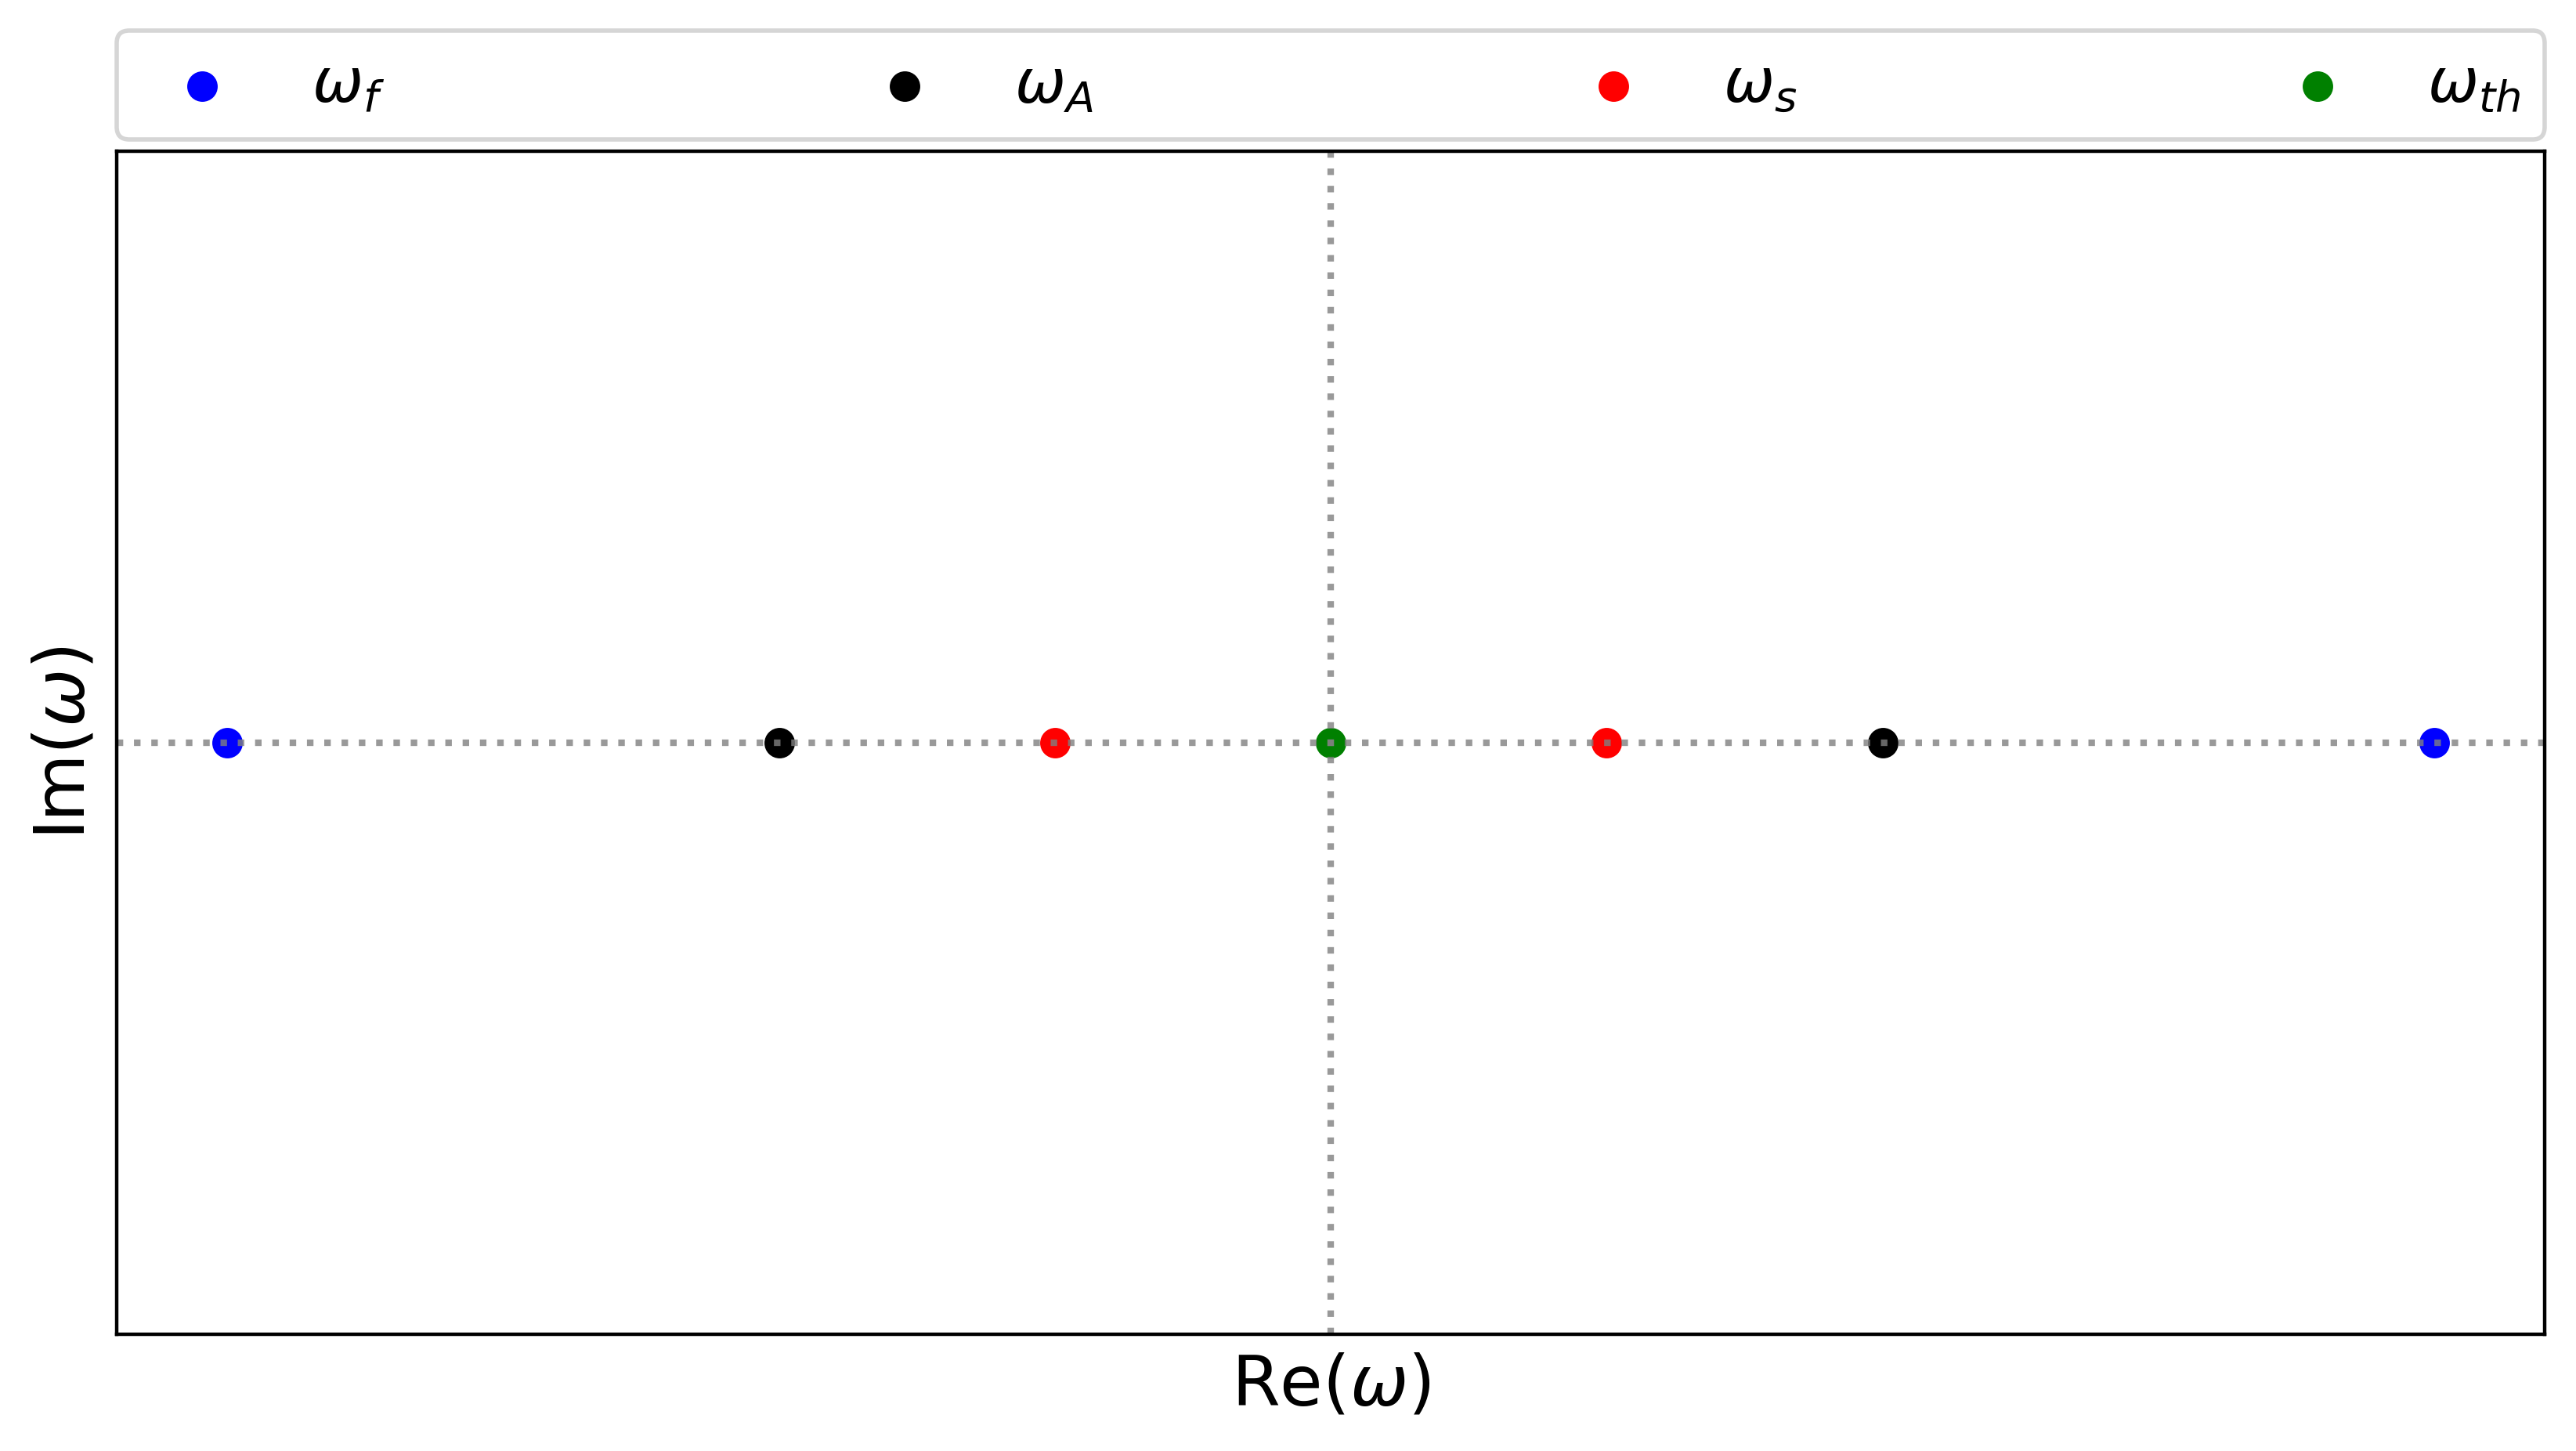
\includegraphics[width=\textwidth]{spectrum_adiabatic.png}
  \caption{
    Visualisation of the ideal MHD spectrum and its seven solutions.
    Blue, black and red dots denote the fast modes, Alfv\'en modes and slow modes, respectively, adhering to the strict ordering in equation \eqref{eq: omega_ordening}. The $\omega = 0$ entropy mode is shown with a green dot, the real and imaginary axes are denoted with dotted lines.
  }
  \label{fig: adiabatic_spectrum}
\end{figure}

\subsection{The non-adiabatic MHD spectrum}
In the previous Subsection we omitted all non-ideal terms in the energy equation \eqref{eq: nonad_energy}, and with the basics in place we can now wonder what will happen to the spectrum when these terms are not omitted. First and foremost, including radiative cooling and/or thermal conduction effects will lift the self-adjointness of the matrix operator, such that genuine complex solutions become possible. The ideal matrix \eqref{eq: ideal_matrix} transforms into its non-adiabatic counterpart
\begin{equation} \label{eq: nonadiabatic_matrix}
  \resizebox{\hsize}{!}{$
    \begin{pmatrix}
      0 & \kperp \rho_0 & 0 & \kpara \rho_0 & 0 & 0 & 0 & 0 \\
      \dfrac{T_0}{\rho_0}\kperp & 0 & 0 & 0 & \kperp & 0 & \dfrac{i B_0}{\rho_0}k_0^2 & 0 \\
      0 & 0 & 0 & 0 & 0 & -\dfrac{\icomplex B_0}{\rho_0}\kpara^2 & 0 & \dfrac{\icomplex B_0}{\rho_0}\kpara \kperp \\
      \dfrac{T_0}{\rho_0}\kpara & 0 & 0 & 0 & \kpara & 0 & 0 & 0 \\
      -\icomplex\gmone \dHLFrho &
        \gmone T_0 \kperp &
        0 &
        \gmone T_0 \kpara &
        -\dfrac{\icomplex\gmone}{\rho_0}\Bigl(K + \rho_0 \dHLFT\Bigr) &
        0 &
        0 &
        0 \\
      0 & 0 & \icomplex B_0 & 0 & 0 & 0 & 0 & 0 \\
      0 & -\icomplex B_0 & 0 & 0 & 0 & 0 & 0 & 0 \\
      0 & 0 & 0 & 0 & 0 & 0 & 0 & 0
    \end{pmatrix},
  $}
\end{equation}
where we defined $K = \kappapara \kpara^2 + \kappaperp \kperp^2$. Before diving into the modifications this brings to the actual spectrum we first take a look at the $v_{1y}$ component. The third row in this matrix can be written as
\begin{equation}
  \omega v_{1y} = -\frac{\icomplex B_0}{\rho_0}\kpara^2 A_{1x} + \frac{\icomplex B_0}{\rho_0}\kpara\kperp A_{1z}.
\end{equation}
If we combine this with the expressions for the $\omega A_{1x} = \icomplex B_0 v_{1y}$ and $\omega A_{1z} = 0$ components, i.e. the sixth and eight rows of the above matrix, the $v_{1y}$ component can be written as
\begin{equation}
  \omega^2 v_{1y} = \frac{B_0^2}{\rho_0}\kpara^2 v_{1y},
\end{equation}
where we assumed that $\omega \neq 0$ since we are interested in non-zero solutions. This expression is, in fact, equal to the one for the Alfv\'en waves in Equation \eqref{eq: alfvenwaves}, completely decoupled from the other equations. This leads us to an interesting conclusion: \emph{Alfv\'en waves in a homogeneous medium remain unaffected by the inclusion of non-adiabatic effects}; their eigenfrequency will remain exactly the same as for the ideal case.

Figure \ref{fig: nonadiabatic_spectrum} shows a typical spectrum for the non-adiabatic case. Open circles denote the adiabatic solutions, solid dots the non-adiabatic modifications. The arrows indicate the direction of ``movement'' in the spectrum. The thermal mode (green) moves away from the origin and becomes unstable, the slow and fast modes become damped in this case, transforming from purely real to genuinely complex solutions.

Generally speaking the non-adiabatic effects included here have opposite trends with respect to stability, that is, thermal conduction will always try to smoothen out temperature gradients and hence (always) has a stabilising effect, while radiative cooling mostly destabilises. The deciding factor here is the dependence of the heat-loss function on temperature $\dHLFT$. There is a direct link between variations in the cooling curve and thermal mode stability: generally speaking strong variations (larger derivatives) lead to a more unstable thermal mode. Where this behaviour comes from, and which role thermal conduction plays in all this, will be extensively discussed in Chapter \ref{ch: thermal instability}.

\begin{figure}[t]
  \centering
  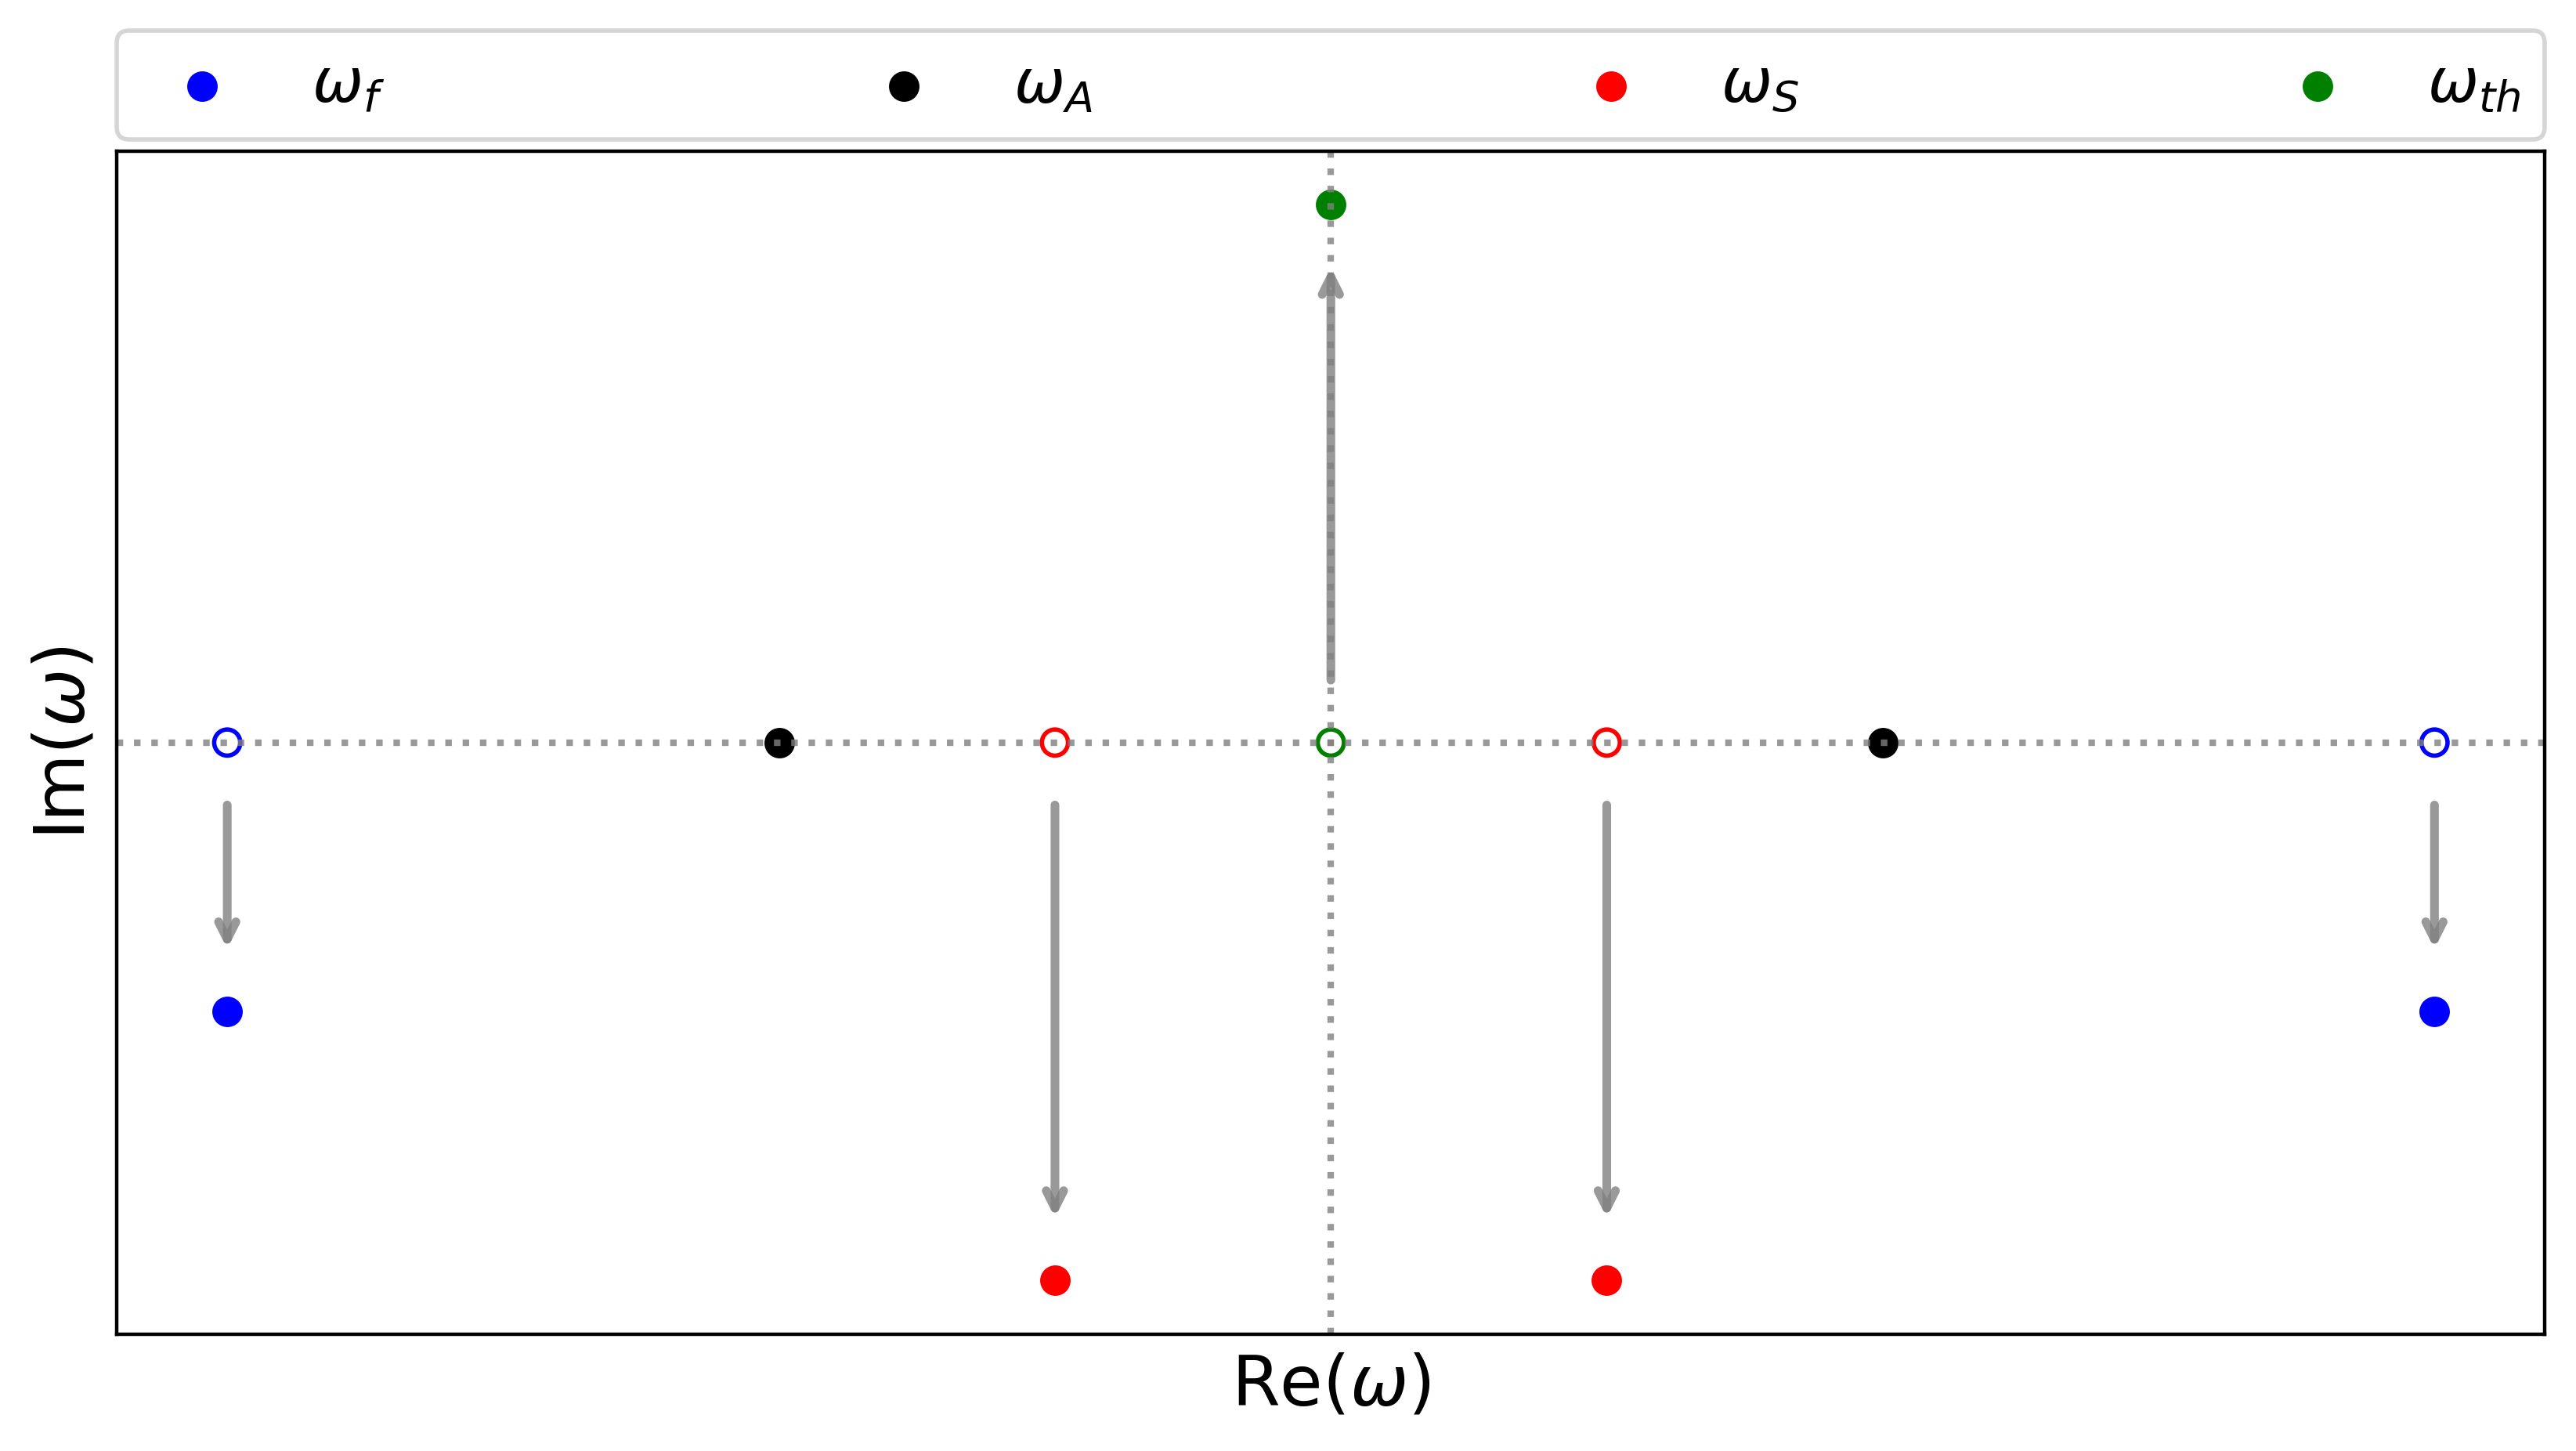
\includegraphics[width=\textwidth]{spectrum_nonadiabatic.png}
  \caption{
    Visualisation of a typical non-adiabatic MHD spectrum; blue, black, red and green dots denote the fast, Alfv\'en, slow and thermal modes, respectively. The empty dots denote the adiabatic solutions, the arrow indicates how these solutions are modified by the additional effects.
  }
  \label{fig: nonadiabatic_spectrum}
\end{figure}


\section{Spectroscopy in non-uniform plasmas}
In all of the above we linearised around a homogeneous background, which allowed us to consider plane-wave perturbations as given in Equation \eqref{eq: plane_wave_homogeneous}. One important remark to be made as well is that the above analysis assumes a medium of infinite extent, i.e. a plasma that is unbounded in all directions.
Nature on the other hand is quite different, since in reality virtually no astrophysical or laboratory plasma configuration is spatially homogeneous, or infinite for that matter. Our initial assumption of uncoupled plane-wave solutions breaks down as soon as we include plasma inhomogeneity, which in turn implies that our operator transformation $\nabla \rightarrow \icomplex\bk$ no longer holds. If we take the direction of inhomogeneity along $x$ then we would have to replace $k_x$ by $\icomplex\partial / \partial x$, and things would get quite complicated real fast. Linearising around a homogeneous background transformed our initial set of partial differential equations to a set of algebraic equations, which could simply be solved by plugging the resulting eigenvalue problem in any modern solver and calculating the eigenvalues. For an inhomogeneous background that depends on $x$ however, the eigenvectors themselves will also depend on $x$, hence all $\nabla$-operators will introduce first (or even second) order derivatives with respect to $x$. This implies that our initial, standard eigenvalue problem $\amat \statevec = \omega \statevec$ will be transformed to a general, complex eigenvalue problem of the form $\amat \statevec = \omega \bmat \statevec$, where the $\amat$ and $\bmat$ matrices \emph{themselves} will contain derivatives of the background quantities, and on top of that the state vector $\statevec$ will contain derivatives of the perturbed quantities as well. At this point most analytical attempts to solve this system will prove impossible and a numerical approach becomes essential.
Before diving into this however, which we will extensively do in Chapter \ref{ch: legolas} and further, we can already familiarise ourselves quite a bit by looking at a relatively simple extension to our homogeneous treatment. This Section builds upon the discussion given in \citet{book_MHD} regarding inhomogeneous plasmas.

\subsection{Spectral symmetry}
Up to now we have neglected to mention a very important property of MHD spectroscopy: that of \emph{spectral symmetry}. This is directly linked to the overall structure of the MHD spectrum, and by extension to the self-adjointness of the matrix operator. These symmetry considerations will remain valid when we later move on to spectroscopy in inhomogeneous plasmas, and have also been partially discussed in \citet{claes2020_legolas}.

We already mentioned a couple of times that the adiabatic linear MHD equations result in a Hermitian eigenvalue problem, hence all eigenfrequencies will be either fully real (stable modes) or fully complex (pure damped or unstable waves) and lie on the real or imaginary axis in the spectral plane. This implies that the full ideal MHD spectrum is \emph{up-down and left-right symmetric}: every mode will have a counterpart mirrored around the corresponding axis, as already seen in Figure \ref{fig: adiabatic_spectrum}. This is directly related to the forward and backwards propagating mode symmetry mentioned earlier, or, equivalently, parity-time symmetry: all these cases are time-reversible.

Including non-ideal effects like radiative cooling and thermal conduction (or e.g. resistivity) lifts the self-adjointness of the eigenvalue problem, allowing the eigenmodes to move away from the axes into the complex plane which will have influence on the symmetry. As long as we are considering static plasmas, that is, no background flow, \emph{left-right symmetry will be preserved}. The inclusion of non-adiabatic effects will however break up-down symmetry as can be seen in Figure \ref{fig: nonadiabatic_spectrum}, but we still have a complementary mode that lies mirrored around the imaginary axis. These spectra correspond to time-irreversible cases.

Finally, including flowing plasmas will introduce a Doppler shift into the spectrum, which in turn is responsible for breaking of left-right symmetry. Ideal, flowing plasmas are in fact governed by a pair of self-adjoint matrix operators \citep{book_MHD}, and every overstable mode has a damped counterpart at the same frequency mirrored around the real axis.

Generally speaking, combining the above statements on spectral symmetry we can summarise as follows:
\begin{itemize}
  \item Static, adiabatic plasmas: \emph{up-down and left-right symmetric}. The eigenvalue problem is Hermitian and all solutions will lie on the real or imaginary axis.
  \item Static, non-ideal plasmas: \emph{left-right symmetric}. The inclusion of non-ideal effects breaks up-down symmetry.
  \item Flowing, adiabatic plasmas: \emph{up-down symmetric}. The Doppler shift introduced by the background flow profile breaks left-right symmetry.
  \item Flowing, non-ideal plasmas: \emph{no symmetry in general}. The combination of flow and non-ideal effects like radiative cooling or resistivity will break left-right and up-down symmetry.
\end{itemize}

From this the wide range in complexity for an MHD spectrum becomes clear: depending on the physical effects taken into account a single spectrum can become extremely complicated. In reality very few astrophysical plasmas can be considered ideal or static, such that in general there will be no spectral symmetry present. In some select cases symmetry can be restored however, even for non-ideal flowing plasmas, by considering a symmetric flow profile in a symmetric domain. This in turn makes the forward and backward modes behave symmetrically, reducing the complexity a bit. This is not always possible however, and generally speaking one will always have to deal with non-symmetric spectra when looking at realistic configurations. In those cases inhomogeneity will also play a major role, which in turn increases the complexity even further due to the presence of the various continua. We will give a general introduction to the MHD continua in Subsection \ref{ss: mhd_continua}.


\subsection{A first approximation to inhomogeneity}
Consider an inhomogeneous medium along $x$ that is bounded between $x = 0$ and $x = L$ but infinite in the $y$ and $z$ directions. As explained in the introductory paragraph we can no longer Fourier analyse along $x$ and a much more intricate treatment is needed. However, we can roughly approximate this medium by a collection of bounded slabs as shown in Figure \ref{fig: bounded_slab} in an effort to understand the general implications that inhomogeneity brings. We can approximately treat the first slab as being bounded between $x = 0$ and $x = a$ and having homogeneous density, temperature and pressure. Due to the bounded nature of this smaller slab the wave number along $x$ will be quantised: $k_x = n\pi / a$ where $n$ is an integer. This in turn introduces a quantisation of the spectrum itself: for every value of $k_x$ we will have a solution to the ideal, homogeneous eigenvalue problem, leading to a discrete spectrum.

\begin{figure}[b]
  \centering
  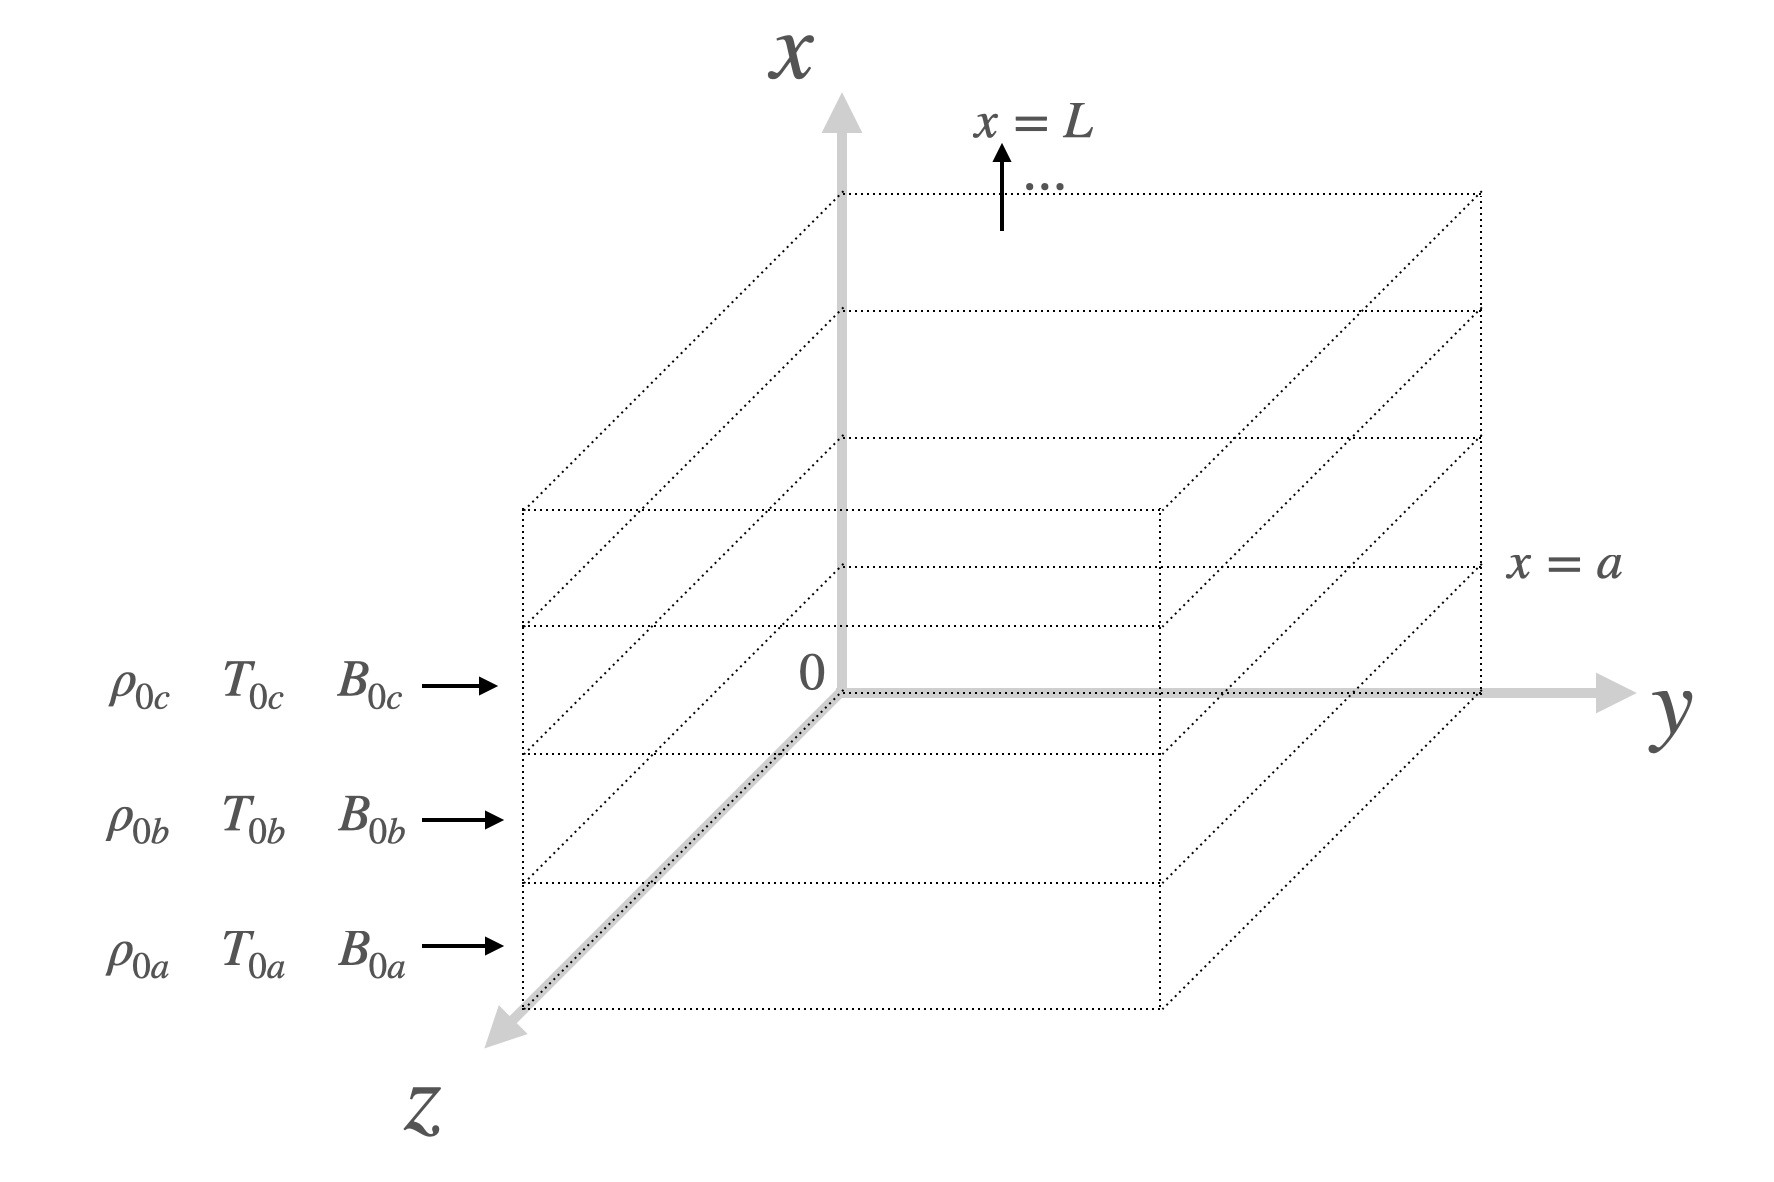
\includegraphics[width=0.7\textwidth]{confined_slab.png}
  \caption{
    An inhomogeneous slab approximated by a collection of homogeneous slabs along $x$, infinite along $y$ and $z$.
  }
  \label{fig: bounded_slab}
\end{figure}

We can understand what this would look like, physically speaking, by turning to the eigenfrequency solutions given in Equations \eqref{eq: alfvenwaves}-\eqref{eq: fs_mhd_waves} while taking the limit of $k_x \rightarrow \infty$. Using the same assumptions as earlier for $\bk$ and $\bb_0$, that is, $\bb_0 = (0, 0, B_0)$ and $\bk = (\kperp, 0, \kpara)$, we get for the Alfv\'en waves
\begin{equation} \label{eq: alfven_accumulation_point}
  \omega_\text{A}^2 = \lim_{\kperp \rightarrow \infty}\omega_\text{a}^2 = \kpara^2\alfvenspeed^2,
\end{equation}
meaning that the Alfv\'en modes are \emph{infinitely degenerate} since they do not depend on $\kperp$. There is hence no difference between $\omega_\text{a}^2$ and $\omega_\text{A}^2$ in this case.

For the slow modes on the other hand we find that
\begin{equation} \label{eq: slow_accumulation_point}
  \omega_\text{S}^2 =
    \lim_{\kperp \rightarrow \infty}\omega_\text{s}^2 =
    \kpara^2 \frac{\alfvenspeed^2 \soundspeed^2}{\alfvenspeed^2 + \soundspeed^2} =
    \frac{\gamma \rho_0 T_0}{\gamma \rho_0 T_0 + B_0^2}\omega_\text{A}^2,
\end{equation}
which, for constant sound- and Alfv\'en speeds (which is the case here as the background is homogeneous), leads to an \emph{accumulation} point in the slow wave sequence. The fast waves have this accumulation point at infinity, since
\begin{equation} \label{eq: fast_accumulation_point}
  \omega_\text{F}^2 = \lim_{\kperp \rightarrow \infty}\omega_\text{f}^2 = \infty.
\end{equation}
Note that we annotated these peculiar frequencies with a capital subscript, as they play a very special role in the eigenspectrum of inhomogeneous plasmas: there the slow accumulation point and degenerate Alfv\'en frequency will get replaced by a continuous range of modes, the slow and Alfv\'en continua, which will be introduced in Subsection \ref{ss: mhd_continua}.

\begin{figure}[t]
  \centering
  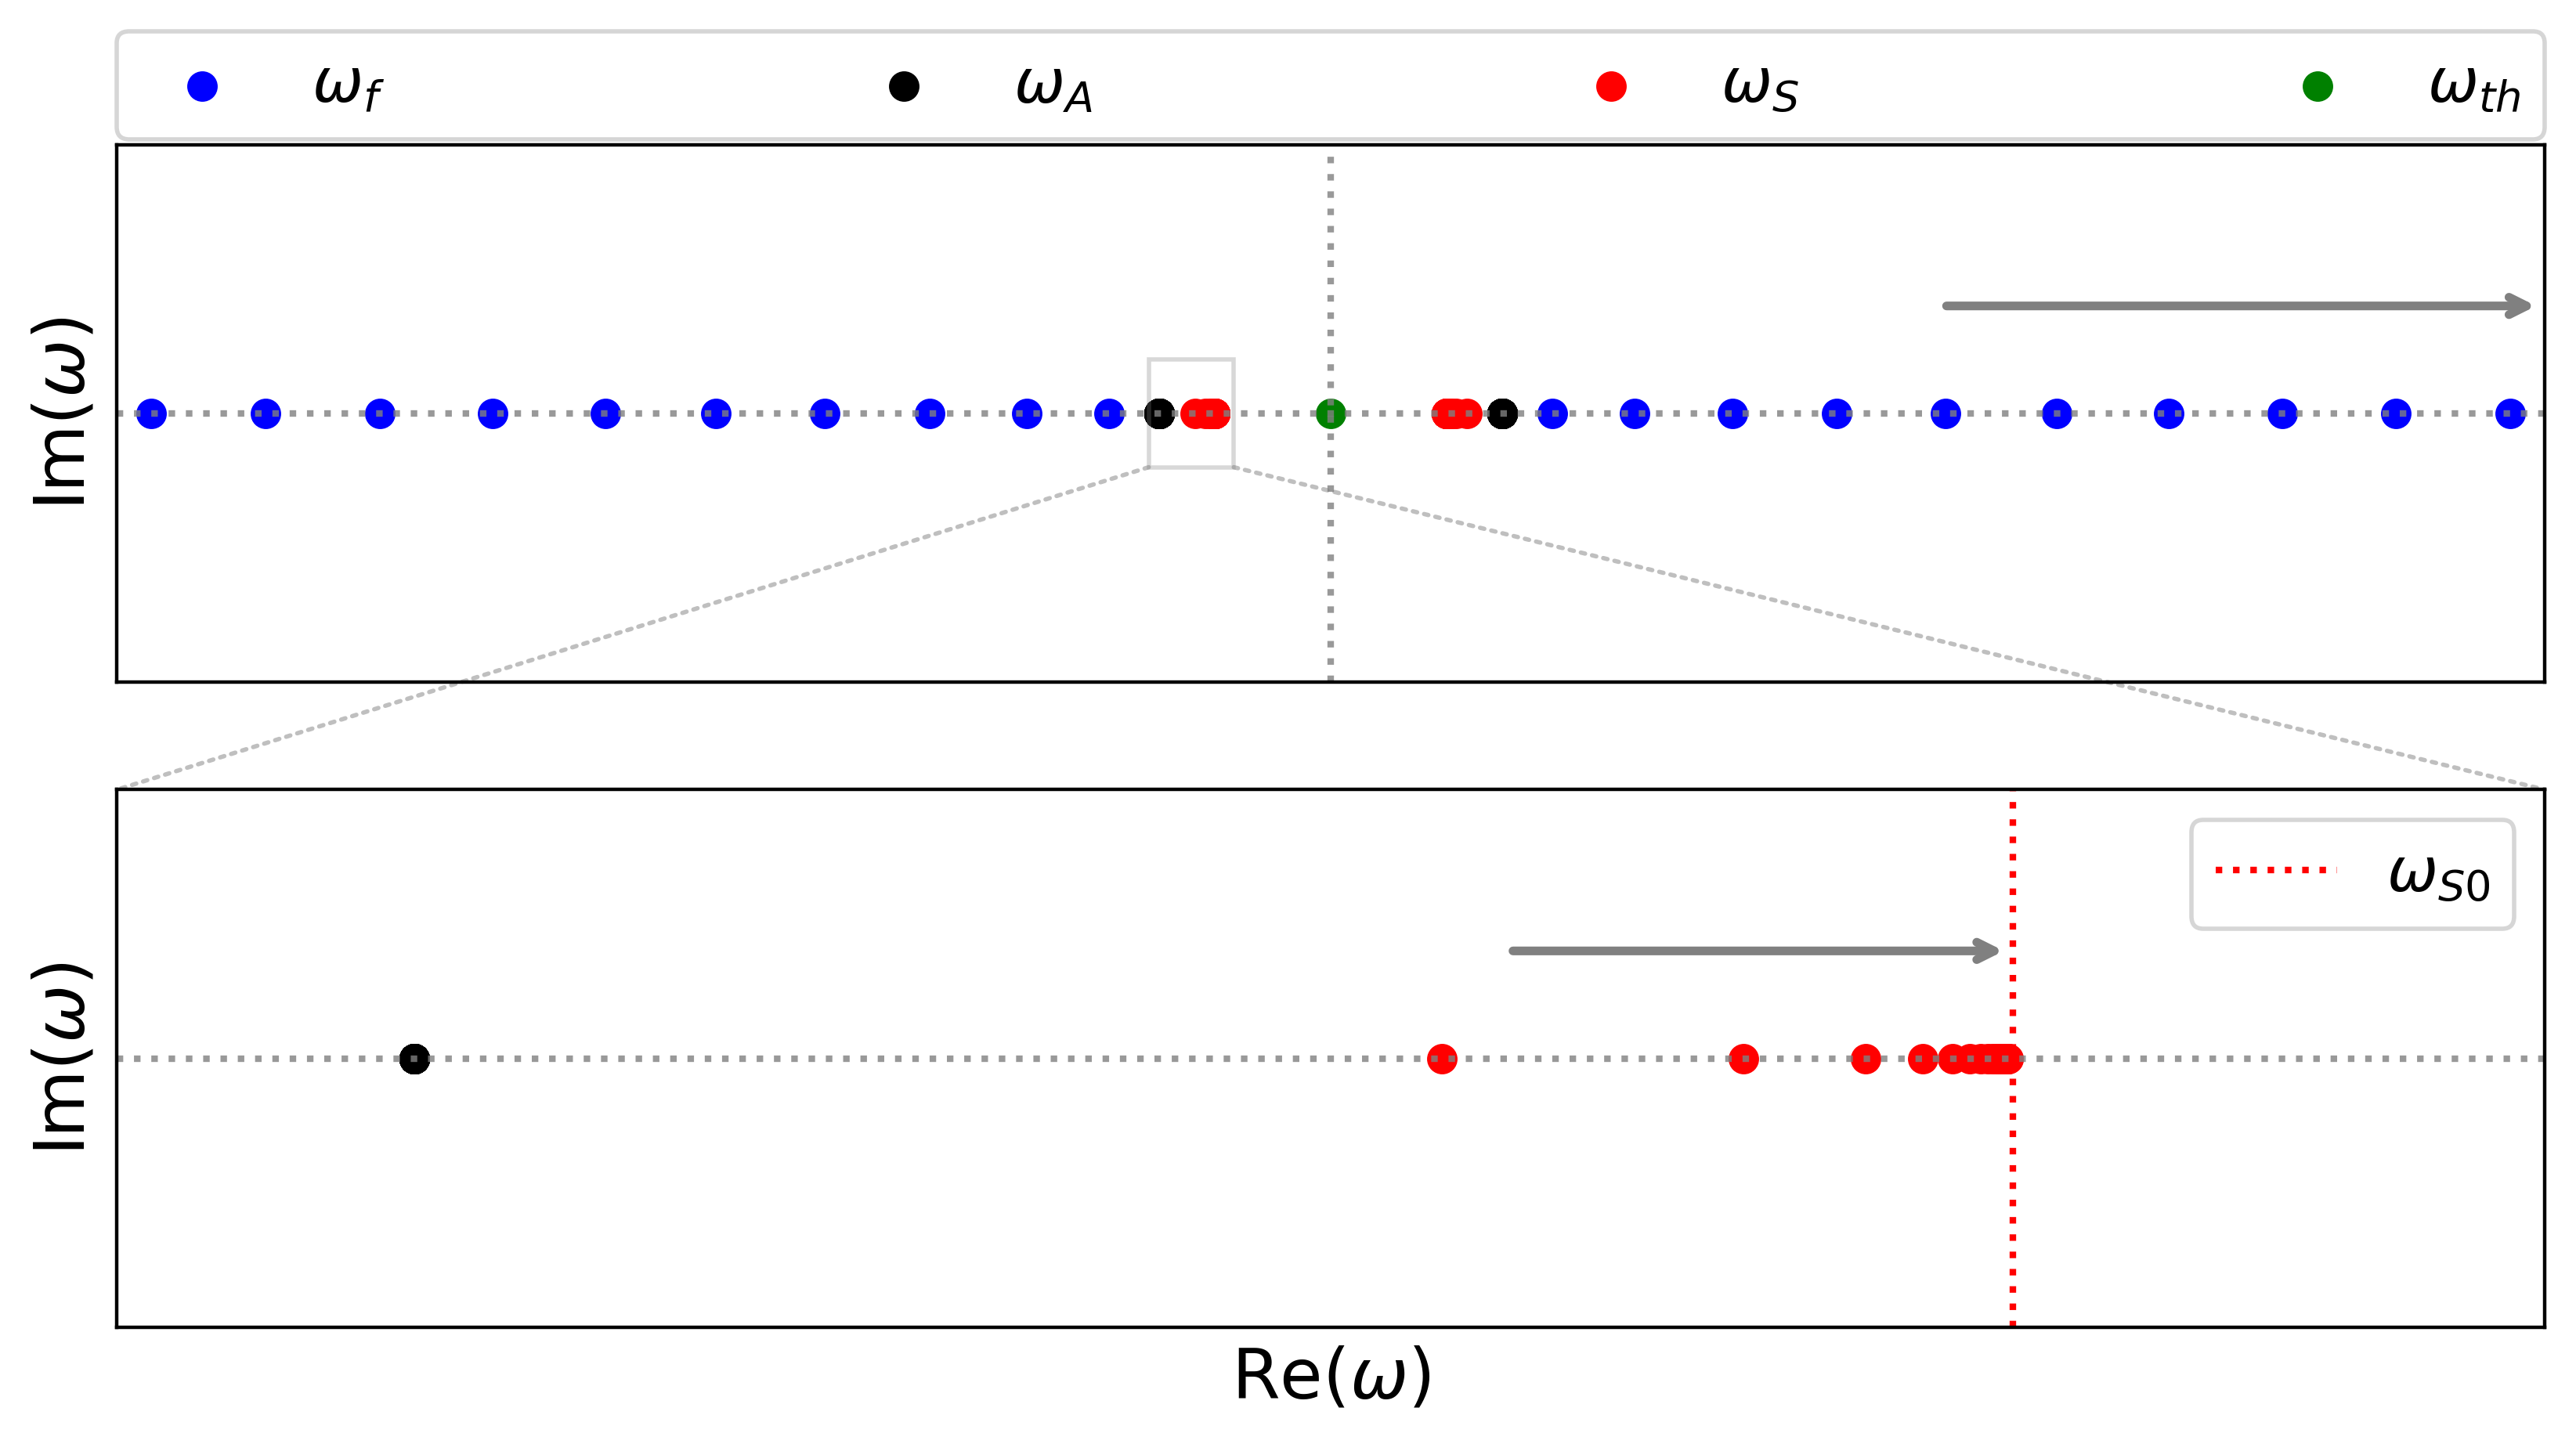
\includegraphics[width=\textwidth]{bounded_ideal_spectrum.png}
  \caption{
    Visualisation of the ideal MHD spectrum for a bounded homogeneous medium. Panel \textbf{a}: overall view of the spectrum, the arrow indicates that the fast modes accumulate at infinity.
    Panel \textbf{b}: zoom of Panel \textbf{a}, clearly showing the degenerate and accumulating behaviour of the Alfv\'en and slow modes, respectively. The slow accumulation point $\omega_\text{S}$ is denoted with a red dotted line, the arrow indicates the direction of increasing $n$.
  }
  \label{fig: bounded_spectrum}
\end{figure}

Figure \ref{fig: bounded_spectrum} shows solutions to the ideal eigenvalue problem, similar to Figure \ref{fig: adiabatic_spectrum}, but for a quantised $\kperp$. Panel a shows an overall view, where the arrow above the fast modes indicates their accumulation point at infinity. Panel b zooms in on Panel a, showing the degenerate behaviour of the Alfv\'en waves and the accumulation sequence of the slow modes. The red dotted line denotes the slow accumulation point $\omega_S$ given by Equation \eqref{eq: slow_accumulation_point}, the arrow indicates the direction of increasing $n$ in the quantisation of the wave number $\kperp$.

\subsection{Introduction to MHD continua} \label{ss: mhd_continua}
\usespublishedwork{
  This Section is partially based on a discussion in the published work ``Magnetohydrodynamic Spectroscopy of a Non-Adiabatic Solar Atmosphere'', 2021, Solar Physics, 296, 9 \citep{claes2021}. N. Claes wrote the manuscript, R. Keppens contributed to the revision of the paper.
}
\subsubsection{Continua in ideal MHD}
To close this Chapter we will briefly touch upon the MHD continua and their (very) important role in the spectral theory of inhomogeneous plasmas. For an inhomogeneous background it is well known that one can reformulate the ideal MHD equations \eqref{eq: ideal_continuity}-\eqref{eq: ideal_induction} into an ordinary differential equation in terms of the $x$-component of the Lagrangian displacement field. It would be rather extensive to do this here, instead we refer to the detailed discussion given in \citet{book_MHD}.

The existence of the slow and Alfv\'en continua correspond to singular points in this ordinary differential equation (ODE), and these continua essentially represent finite ranges of eigenfrequencies with singular, ultra-localized eigenfunctions. They play a key role in processes like phase mixing, resonant absorption or uniturbulence processes. In ideal MHD, the forward and backward slow and Alfv\'en continua are always real (pure waves), and the eigenfrequency ranges are $x$-dependent when the direction of inhomogeneity in the background is taken along $x$.

The slow, Alfv\'en and fast accumulation points discussed in Equations \eqref{eq: alfven_accumulation_point}-\eqref{eq: alfven_accumulation_point} are actually special situations originating from these continua, in which the continua collapse to degenerate single points in homogeneous media. An intuitive way to look at this is to consider the expression for the Alfv\'en accumulation point $\omega_\text{A}^2 = \kpara^2\alfvenspeed^2$, which depends on the Alfv\'en speed and by extension on the density and magnetic field profiles. For an inhomogeneous background these profiles will depend on $x$, hence the Alfv\'en speed will vary over the domain, and thus the continua as well giving rise to a finite range in eigenfrequency. The same reasoning holds for the slow continuum, and since the fast modes have their accumulation point at infinity (such that they don't give rise to singular points in the ODE) we do not have a ``fast continuum''. Additionally, when viewed as a function of $x$, local minima or maxima in the continua may lead to the presence of additional, discrete sequences of modes that cluster towards these accumulation ranges.

\subsubsection{Continua in non-adiabatic MHD}
The inclusion of non-adiabatic effects introduces the thermal continuum, which in static, non-adiabatic settings is just the entropy (thermal) mode. It was shown by \citet{vanderlinden1991} that these continuum modes are introduced by $\kappaperp = 0$, and hence only exist if there is no thermal conduction perpendicular to the magnetic field lines. For nonzero $\kappaperp$ the thermal continuum gets replaced by a quasi-continuum, represented by a dense band of discrete thermal modes. The Alfv\'en continuum remains unmodified when only non-adiabatic effects are included and hence all its continuum solutions will be real, corresponding to locally resonant waves. The slow continuum on the other hand is modified and couples to the thermal continuum, with solutions given by a third-order polynomial in $\omega$
\begin{equation}	\label{eq: slow_thermal_continuum}
  \frac{\rho_0 \left(\soundspeed^2 + \alfvenspeed^2\right)}{\gamma - 1}\icomplex\omega^3
  + \Qai\omega^2
  - \frac{\rho_0 \soundspeed^2\alfvenspeed^2 \kpara^2}{\gamma - 1}\icomplex\omega
  - \Qi\alfvenspeed^2 \kpara^2 = 0,
\end{equation}
with $\isosoundspeed^2 = p_0 / \rho_0$ the isothermal sound speed. The quantities
\begin{equation}
  \begin{gathered}
	  \Qi = \Qifull, \\
    \Qai = \Qaifull,
  \end{gathered}
\end{equation}
are introduced for brevity. Generally speaking, Equation \eqref{eq: slow_thermal_continuum} usually has one purely imaginary solution, corresponding to the thermal continuum $\omega_\text{th}$, and two complex conjugate solutions representing the slow continua $\omega_\text{S}^\pm$. In the ideal case the constant term and the $\omega^2$ term collapse to zero, such that $\omega_\text{th}$ vanishes (reducing to the marginal entropy solution $\omega_\text{th} = 0$). The slow continua reduce to their ideal counterparts $\omega_\text{S}^2 = \kpara^2\soundspeed^2\alfvenspeed^2/(\soundspeed^2 + \alfvenspeed^2)$, which may in turn collapse into points if $\soundspeed$ and $\alfvenspeed$ are both not spatially varying. If the slow continuum vanishes, which is the case if $\bk \cdot \bb_0 = 0$ or if a pressureless background is considered (that is, adopting a zero plasma-$\beta$), the thermal continuum has an analytical solution given by
\begin{equation}
	\omega_\text{th} =
    \frac{\gmone\icomplex}{\soundspeed^2 + \alfvenspeed^2}
    \left[\rho_0\dHLFrho - \dHLFT\left(\isosoundspeed^2 + \alfvenspeed^2\right)\right],
\end{equation}
and hence becomes independent of thermal conduction effects.

\subsubsection{Stability implications of the continua}
It is really important to stress that continuum modes are in fact \emph{actual solutions} to the eigenvalue problem, and hence represent physical modes. Consequently, one can draw the following general conclusions for the stability of a given equilibrium, solely based on the behaviour of its slow and/or thermal continuum regions:

\begin{itemize}
	\item[i)] The continuum regions are partially or fully unstable, that is at least some continuum modes have a positive imaginary part. Since these modes are physical solutions, this means that the medium will be susceptible to instability, either through an unstable slow or thermal mode (or a coalescence of both) depending on which continuum region is unstable. How fast these instabilities form will (usually) depend on the growth rates of the most unstable mode(s), although mode interactions and nonlinear effects can develop quickly.
	\item[ii)] The continuum regions have no internal extrema and are completely stable, that is all modes have a negative or vanishing imaginary part. This corresponds to a stable case, where there is no possibility to trigger instability.
	\item[iii)] The continuum regions have internal extrema. This represents the more general case, in which discrete modes in the vicinity of the continua \textit{may} exist. Here it is possible to have a stable continuum with an unstable discrete mode such that the medium is still unstable.
\end{itemize}

The role of these continua will become clear when we start discussing spectra of inhomogeneous configurations in Chapters \ref{ch: legolas} and \ref{ch: legolas_applications}.

\cleardoublepage

\chapter{Spectroscopy in homogeneous plasmas} \label{ch: homogeneous_plasmas}


\cleardoublepage

\chapter{The finite element code Legolas} \label{ch: legolas}

\graphicspath{{04-legolas/figures/}}

\begin{chapterquote}[Stephen Hawking][A Brief History of Time][]
  Any physical theory is always provisional, in the sense that it is only a hypothesis; you can never prove it. No matter how many times the results of experiments agree with some theory, you can never be sure that the next time the result will not contradict the theory.
\end{chapterquote}

\usespublishedwork{
  Parts of this Chapter were published in ``Legolas: a novel tool for magnetohydrodynamic spectroscopy'', 2020, \apjs,
  251, 25 \citep{claes2020_legolas}. N. Claes developed {\legolas} in close collaboration with J. De Jonghe, generated the data and figures and wrote a first draft of the manuscript; J. De Jonghe revised and extended the manuscript. R. Keppens contributed to the revision of the paper.
}

In the previous Chapter we looked at wave modes and growth rates in simple planar, uniform configurations. Naturally, the next step would be adding a continuous, spatial variation in the background equilibrium prescription, allowing us to investigate wave modes in inhomogeneous media. An approach like this is essential if we ever hope to discuss more realistic configurations, which indirectly implies that we ought to look at curved geometries as well, that is, cylinders instead of slabs. Mathematically speaking, this ``small'' step is actually a major undertaking: while this allows for a relatively accurate description of various realistic equilibrium configurations, it also means that the mathematical analysis increases (a few orders of magnitude) in complexity. It will not take long before we have to forego any hopes of a general analytic treatment and are forced to turn to numerical tools.

With this in mind we embarked on an ambitious project: develop a new, large-scale numerical code to solve the linearised system of non-ideal MHD equations. In the past few decades various codes have been developed for exactly this purpose, but these were limited: some versions applied severe constraints on the physical effects that could be added -- for example \emph{only} resistivity, or \emph{only} non-adiabatic effects -- while others looked only at specific configurations and built their code for that specific purpose. {\legolas} on the other hand has one main vision: provide a framework that is as general as possible; while at the same time easy to extend with additional physics or modern algorithmic developments. The result is that we now have a single, modern, and modular code, capable of doing spectroscopy on configurations that have never been investigated before, whilst combining physics that have never been combined before in MHD spectroscopy.

This Chapter provides the mathematical foundations on which the {\legolas} code is built. We look at the linearisation process and how it affects the physical terms taken into account, followed by a thorough discussion on the actual eigenvalue problem and how the mathematical and numerical challenges have been overcome.
Section \ref{sec: problem description} introduces the system of equations, along with the linearisation procedure and Fourier mode representation. In Section \ref{sec: eigenvalue problem} we explain the mathematical formalism behind Finite Element Methods (FEM), with a complete treatment of the finite element matrix assembly process, boundary conditions and assembly of the eigenfunctions from the calculated eigenvectors.

\section{Introduction}
The study of stability for plasmas and fluids alike has been a major topic of research over the last century. Understanding how and why a given medium reacts to a linear perturbation is of central importance to many astrophysical phenomena. In incompressible or compressible fluids, governed by the hydrodynamic equations, notable instabilities are the Kelvin-Helmholtz instability (KHI), which arises due to a velocity shear at the interface of two fluids, and the Rayleigh-Taylor instability (RTI) where gravitational stratification can lead to an unstable configuration of layered fluids of different density \citep{book_chandrasekhar,book_choudhuri}. In plasmas, governed by the magnetohydrodynamic equations, the study of waves and instabilities becomes much richer due to the inclusion of magnetic fields, with a modern overview provided in \citet{book_MHD}. Magnetic fields modify the two aforementioned instabilities in various ways, and the combination of flow, magnetic fields and pressure gradients introduces many new modes, e.g. the magnetorotational instability \citep{balbus1991} relevant for (weakly magnetised) accretion disks or the trans-slow-Alfv\'en continuum modes in disks of arbitrary magnetisation \citep{goedbloed2004}. In the highly magnetised solar corona, observed coronal loop oscillations (periods and damping times) are routinely used to infer loop parameters like their field strength \citep{nakariakov2001}. Embedded in the hot solar corona, we find stable and long-lived quiescent prominences, with internal dynamics due to KHI \citep{hillier2018_KHI} and RTI \citep{hillier2018_RTI}. The formation of prominences is due to the thermal instability, as demonstrated in direct observations by e.g. \citet{berger2012} or in simulations by \citet{xia2016} and \citet{claes2020}. Together with categorising all instabilities, knowing the stable eigenoscillations, such as $p$ or $g$ modes in stratified atmospheres or stellar interiors, is of prime importance to link theoretical understanding with observed periodic phenomena. In all of these cases, we need to compute the eigenoscillations and corresponding eigenfunctions from the linearised set of governing equations. Linear MHD spectroscopy, which encompasses the entirety of helio- and asteroseismology but incorporates laboratory fusion plasma MHD spectroscopy \citep{goedbloed1993}, MHD spectroscopy of accretion disks \citep{keppens2002} and jets, as well as solar coronal seismology \citep{book_roberts}, is thus a powerful tool for studying many astrophysical processes.

Since the advent of more powerful computational resources, the main focus of computational astrophysical research has gradually shifted toward solving the fully nonlinear MHD equations, where many nonadiabatic/nonideal effects are incorporated, depending on the application at hand. While this approach successfully reproduces many physical phenomena, especially for realistic solar setups (e.g. sunspots, \citet{rempel2012}; flares, \citet{ruan2019}; or prominences, \citet{xia2016}), it usually fails to answer which specific perturbation produces the complex evolution as witnessed. At the same time, theoretical insight showed that MHD spectral theory actually governs the stability of flowing, (self-)gravitating single-fluid evolutions of nonlinear, time-dependent plasmas, and this at any time during their nonlinear evolution \citep{demaerel2016}. Hence, in order to predict the reaction of a certain physical state to perturbations, we should really quantify all its waves and instabilities using linear theory. This has been recognised fully in laboratory fusion plasmas, where MHD spectroscopy is very successful in identifying waves and stability aspects of a given toroidal Grad-Shafranov equilibrium. That this can be meaningfully be done for states that include important nonadiabatic effects, like optically thin radiative losses, is important for investigations into prominences and their intriguing fine structure, as revealed by means of direct observations \citep{engvold1998,ballester2006,mackay2010} or through numerical simulations \citep{xia2016,xia2017,claes2020}. In that context, early analytical work by \citet{vanderlinden1991} based on linear MHD suggests the hypothesis that finite perpendicular thermal conduction induces fine structure in unstable linear eigenmodes. Since this pioneering work of \citet{vanderlinden1991}, not much research has been done regarding the full MHD spectrum where nonadiabatic effects are at play, for the simple reason that to date, there existed no numerical tool to solve the full system of linearised MHD equations with all the physical effects included. Additionally, for typical astrophysical plasmas the conditions are far from static: tokamak plasmas, astrophysical jets, solar coronal loops, accretion disks, etc., all have equilibrium flows. The combination of flow and nonadiabatic effects, where both left-right and up-down eigenfrequency symmetries are broken, has never been explored in earnest. This makes it clear that a numerical approach becomes essential, especially when the equilibrium is no longer homogeneous. Because in reality virtually no astrophysical configuration is spatially homogeneous, we need a flexible numerical tool to explore the spectrum systematically. This is why we developed a completely new and open-source code, which we named {\legolas}, an acronym for ``Large Eigensystem Generator for One-dimensional pLASmas''.

{\legolas} builds on the heritage of early numerical codes, most notably LEDA \citep{kerner1985}, which allowed studies of the ideal or resistive MHD spectrum for laboratory plasmas, approximated by a diffuse cylindrical plasma column (or flux tube) and CASTOR \citep{kerner1998}, which applied to resistive spectra of general tokamak configurations. The latter has follow-up codes such as FINESSE \citep{belien2002} and PHOENIX \citep{blokland2007_phoenix}, extending it to stationary and axisymmetric truly 2D configurations. LEDA was later extended by \citet{vanderlinden1992}, where nonadiabatic effects like anisotropic thermal conduction and optically thin radiative losses were added to the equations using a simple analytic function to treat radiative cooling effects. A different branch of LEDA, called LEDAFLOW \citep{nijboer1997}, was developed to investigate the resistive MHD spectrum, augmented with gravitational and flow effects, but omitting those nonadiabatic terms. Because these codes were developed decades ago and focus has shifted away from linear MHD, their further development was stalled, although in laboratory fusion context, tools to compute multidimensional equilibria and their linear modes are very important for diagnosing experiments. The original codes, like LEDA(FLOW), were not flexible in the sense that adding different equilibria or accounting for additional terms in the equations would be a major undertaking, as parts were hard-coded to (limited) computational resources of that time. Furthermore, programming languages and numerical tools like LAPACK \citep{book_lapack} to solve eigenvalue problems have come a long way.

The {\legolas} code is able to handle both Cartesian and cylindrical geometries, and introduces many new features, such as selecting between modern cooling curves that treat optically thin radiative cooling effects. Furthermore, every aspect of the code is modularised, making it ready to be extended with additional physics or modern algorithmic requirements such as mesh refinement. The main goal of this Chapter is to discuss the mathematical foundations behind the {\legolas} framework. {\legolas} solves the linearised MHD equations including various nonadiabatic effects and (among others) resistivity and gravity assuming a one-dimensional (1D) equilibrium profile with the possibility of a background flow. A standard Fourier analysis for the perturbations is combined with a finite element representation of the eigenfunctions in the important coordinate. The original system is transformed into an eigensystem for the complex eigenfrequencies $\omega$. We make use of a general formalism to include two kinds of geometries: a plane Cartesian stratified slab or a (possibly also stratified) cylinder, through the inclusion of a scale factor originating from the divergence, gradient, and curl operators. {\legolas} can handle the hydrodynamic limit (where all equilibrium magnetic field components are set to zero), enabling us to investigate the stability of hydrodynamic static and stationary equilibria as well. The resulting system of equations is solved in weak form, transforming the original system into a non-Hermitian complex eigenvalue problem, which is then solved. This results in a calculation of all eigenfrequencies and corresponding eigenfunctions of the system, such that a detailed analysis of mode stability -- but also the entire overview on all supported linear wave modes -- becomes possible.


\section{Problem description and equations} \label{sec: problem description}
In this Section we will develop the mathematical formalism leading up to the set of linearised equations. The inhomogeneous equilibrium profiles under consideration make the linearisation process much more complicated compared to Chapter \ref{ch: spectroscopy}, and we also include a lot more physical effects than before.

\subsection{Full set of MHD equations}
We start from the same set of MHD equations as in Chapter \ref{ch: spectroscopy}, but now we include a gravitational field, resistivity, and background flow effects, in addition to optically thin radiative losses and anisotropic thermal conduction. This implies that the initial set of MHD equations expands into
\begin{flalign}
  \frac{\partial \rho}{\partial t} &= -\nabla \cdot (\rho \bv), \label{eq: continuity} \\
  \rho\frac{\partial \bv}{\partial t} &=
    -\nabla p - \rho \bv \cdot \nabla \bv + (\nabla \times \bb) \times \bb + \rho\bg,	\label{eq: momentum} \\
  \rho\frac{\partial T}{\partial t} &=
    -\rho \bv\cdot\nabla T - \gmone p\nabla \cdot \bv - \gmone\rho\HLF
    + \gmone\nabla \cdot (\bkappa \cdot \nabla T) \label{eq: energy} \\
    &\quad + \gmone\eta(\nabla \times \bb)^2, \nonumber \\
  \frac{\partial \bb}{\partial t} &=
    \nabla \times (\bv \times \bb) - \nabla \times (\eta\nabla \times \bb). \label{eq: induction}
\end{flalign}
Here $\eta$ denotes the resistivity and $\bg$ the gravitational acceleration.

\subsection{Linearisation of the physical terms}
\subsubsection{Equilibrium background}
Just as in Chapter \ref{ch: spectroscopy} we linearise the above set of MHD equations, meaning we first have to specify a background which in this case will no longer be homogeneous. Since we want our mathematical formalism to be quite general, we consider a coordinate system denoted by $(u_1, u_2, u_3)$, corresponding to three orthogonal basis vectors. The main advantage of this approach is that it allows us to include two different geometries with only one basic formalism (and implementation). First we consider a standard plane slab geometry in Cartesian coordinates, that is, a plasma which is confined in height and considered to be bounded by two horizontal, perfectly conducting walls at a fixed distance apart, extending outwards to infinity in the other two ignorable coordinates. This also approximates the limit of a fully infinite free space when the walls are moved off to infinity. In Cartesian geometry the coordinate system can be written as $(x, y, z)$ and the vectors $\{\uunit{1}, \uunit{2}, \uunit{3}\}$ are then the standard Cartesian triad $\{\unit{x}, \unit{y}, \unit{z}\}$ along the axes. This makes it quite convenient to include for example gravitational effects which will induce an equilibrium stratification in the $u_1$ coordinate. The second geometry under consideration is that of an infinitely long plasma cylinder encased by a solid wall at a certain radius away from the cylinder axis, for which the coordinate system can be defined as $(r, \theta, z)$. At each point the vectors $\{\uunit{1}, \uunit{2}, \uunit{3}\}$ are defined as the triad of tangent vectors, $\{\unit{r}, \munit{\theta}, \unit{z}\}$, with $\unit{r}$ along the radial direction, $\unit{z}$ in the direction of the cylinder axis and $\munit{\theta} = \unit{z} \times \unit{r}$ tangent to the cylinder.
The basic operators present in Equations \eqref{eq: continuity}--\eqref{eq: induction}, that is, the divergence, gradient and curl, introduce a factor $r$ when going from Cartesian to cylindrical coordinate systems. To make life easy we can introduce the \emph{scale factor} $\eps = r$ for cylindrical geometries, which is reduced to $\eps = 1$ for a Cartesian coordinate system. Hence exploiting this scale factor in the mathematical formalism allows for one single implementation, where one can conveniently switch between both cases. We note that the cylindrical setup is also applicable to the so-called cylindrical accretion disk limit, as for example exploited to study MHD instabilities in disks by \citet{blokland2007}.

{\legolas} handles one-dimensional equilibria which depend only on $u_1$, or, more specifically, time-independent equilibria of the form
\begin{equation}	\label{eq: legolas_equilibrium}
	\begin{aligned}
		\rho_0 &= \rho_0(u_1),		\\
		p_0 &= p_0(u_1),			\\
		T_0 &= T_0(u_1),			\\
	\end{aligned}
	\qquad\qquad
	\begin{aligned}
		\bv_0 &= v_{01}(u_1)\uunit{1} + v_{02}(u_1)\uunit{2} + v_{03}(u_1)\uunit{3},	\\
		\bb_0 &= B_{01}\uunit{1} + B_{02}(u_1)\uunit{2} + B_{03}(u_1)\uunit{3}. \\
		&
	\end{aligned}
\end{equation}
In general we have $\bg = -g(u_1)\uunit{1}$, where the Cartesian case is for a stratified atmosphere or layer, and the cylindrical case can also allow for gravitational stratification of an accretion disk situated for $u_1 = r \in [1, R]$. In the case of a cylinder where $u_1 = r \in [0, R]$, this gravitational term is absent. The presence of a $u_1$-dependent $\uunit{1}$ component in the velocity field allows for compressible background flows, that is, $\nabla \cdot \bv_0 \neq 0$. It should be noted that in order for $\nabla \cdot \bb_0 = 0$ to hold, we actually need $B_{01}/\eps$ as $\uunit{1}$ component for the magnetic field, which reduces to the constant $B_{01}$ in Cartesian geometries and $B_{01}/r$ for cylinders. However, we will not consider the latter case as it will introduce even more terms in the equations, hence at the time of writing {\legolas} only allows for a non-zero $B_{01}$ component in Cartesian slabs.

\begin{figure}[t]
  \centering
  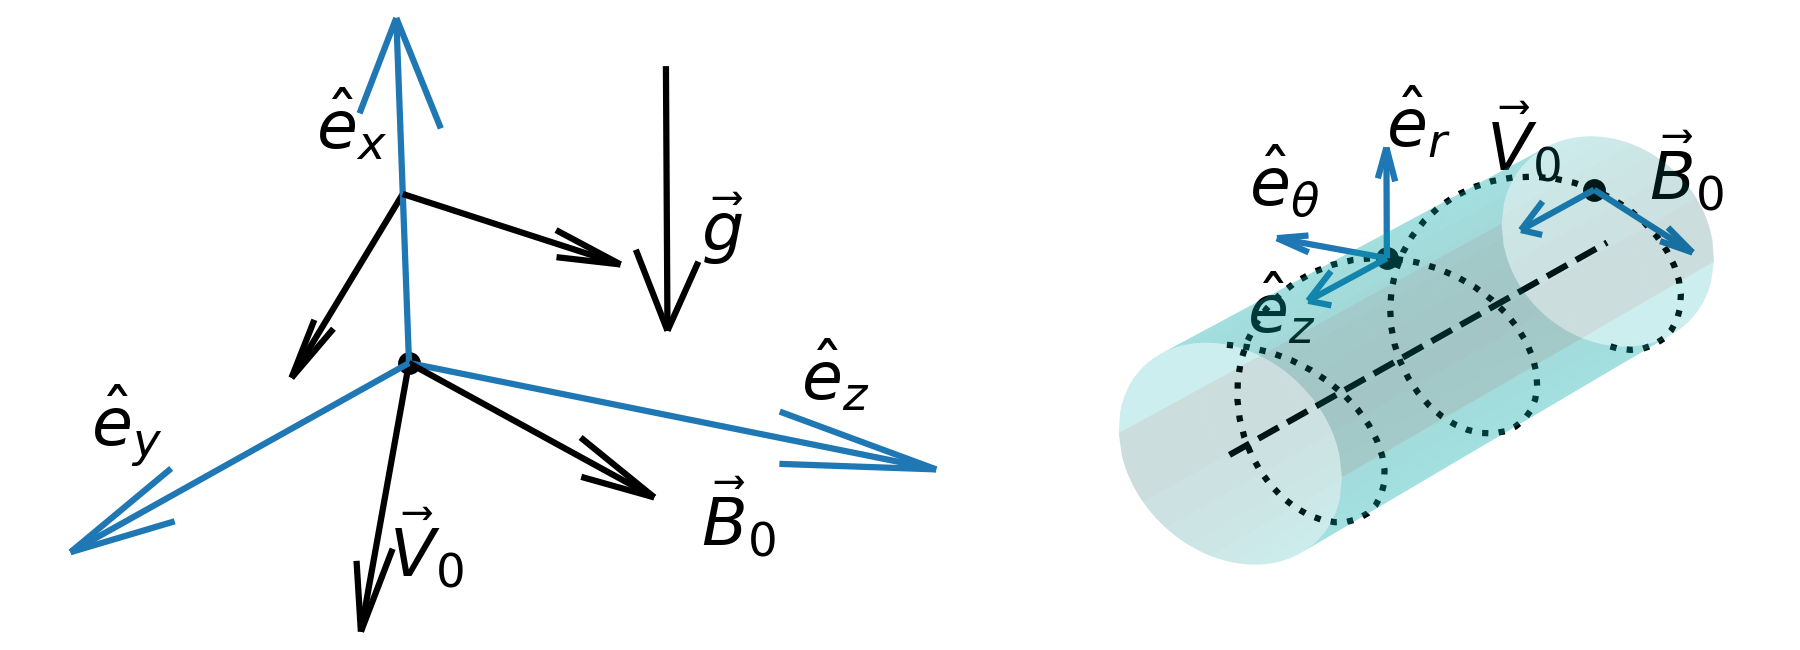
\includegraphics[width=\textwidth]{coordinate_axes.png}
  \caption{
    Unit vectors and examples of $\bb_0$ and $\bv_0$ for the Cartesian (\textbf{left}) and cylindrical (\textbf{right}) cases. These correspond to the general formalism given by Equation \eqref{eq: legolas_equilibrium}
    with $v_{01} = B_{01} = 0$.
  }
  \label{fig: coordinate_axes}
\end{figure}

In what follows the $v_{01}(u_1)$ and $B_{01}$ terms are included in the mathematical formalism for completeness, but will be set to zero in all applications discussed in the remainder of this thesis. Essentially, this implies that the general formalism in Equation \eqref{eq: legolas_equilibrium} reduces to the configuration shown on Figure \ref{fig: coordinate_axes}.

\subsubsection{Resistive terms}
The resistivity contribution in the energy equation is given by $\gmone \eta (\nabla \times \bb)^2$, which can be straightforwardly linearised as
\begin{equation}
  \begin{gathered}
    \gmone\left(\eta_0 + \eta_1\right)\left(\nabla \times \bb_0 + \nabla \times \bb_1\right)^2 \\
    \simeq 2\gmone \eta_0 \left(\nabla \times \bb_0\right) \cdot \left(\nabla \times \bb_1\right)
      + \gmone\eta_1 \left(\nabla \times \bb_0\right) \cdot \left(\nabla \times \bb_0\right),
  \end{gathered}
\end{equation}
in which the nonlinear terms and equilibrium contributions were omitted. For the resistivity $\eta$ one can in principle take any profile, {\legolas} implements the Spitzer resistivity given by
\begin{equation} \label{eq: spitzer_eta}
  \eta = \frac{4\sqrt{2\pi}}{3}\frac{
    Z_\text{ion} \electroncharge^2 \sqrt{\masse} \ln(\lambda)
  }{
    \left(4\pi\epsilon_0\right)^2\left(\boltzmanncte T\right)^{3/2}
  },
\end{equation}
where $Z_\text{ion}$ denotes the ionisation taken to be unity, $\electroncharge$ and $\masse$ denote the electron charge and mass, respectively, and $\epsilon_0$ and $\boltzmanncte$ are the electrical permittivity and Boltzmann constant. The Coulomb logarithm is given by $\ln(\lambda)$ and is approximately equal to 22 for solar coronal conditions \citep{book_MHD}. It is important to emphasise that, since we will further linearise the governing nonlinear equations, we can adopt fully realistic values for all the nonideal coefficients, such as the resistivity or thermal conduction coefficients. This is in contrast to fully nonlinear computations, which are severely restrained in reaching magnetic Reynolds numbers $\magneticreynolds$ beyond $10^4$--$10^5$. The assumption of Spitzer resistivity implies that the perturbed part $\eta_1$ can be written in terms of perturbed temperature as
\begin{equation}
  \eta_1 = \left.\frac{d\eta}{dT}\right|_{T_0}T_1.
\end{equation}

In addition to this {\legolas} allows for an anomalous resistivity prescription in which we typically have $\eta(\uunit{1}, \boldsymbol{j}(\uunit{1}, t))$, that is, a resistivity profile that is spatio-temporal in general, but for a fixed time, depends on position and current profile. This in turn implies that a total derivative should be used for the resistivity, given by
\begin{equation}
  \eta' = \frac{\partial \eta}{\partial u_1} + T_0'\frac{\partial \eta}{\partial T},
\end{equation}
when calculating the derivative with respect to $u_1$. In most use cases a resistivity profile $\eta(T(\uunit{1}))$ is sufficient however, which is only temperature dependent -- and hence indirectly spatially varying as well for inhomogeneous temperature profiles.

\subsubsection{Optically thin radiative losses}
Just as before the optically thin radiative losses are governed by the heat-loss function $\HLF$, and the radiative cooling term $\gmone \rho \HLF$ in the energy equation can be linearised as
\begin{equation}
  \gmone \rho_1 \HLF_0 + \gmone \rho_0 \HLF_1.
\end{equation}
This time however we generalise the formalism to include a density and temperature-dependent heating function
$\HLFheat(\rho, T)$, that is,
\begin{equation}
  \HLF = \rho\HLFcool - \HLFheat(\rho, T).
\end{equation}
{\legolas} has multiple cooling curves implemented, most notably {\jccorona} and {\spexdm} as shown on Figure \ref{fig: coolingcurves}. In addition a piecewise power law as described by \citet{rosner1978} is also implemented, which is an explicit (piecewise) function over the entire temperature domain.

\subsubsection{Anisotropic thermal conduction}
The thermal conduction term $\nabla \cdot (\bkappa \cdot \nabla T)$ in the energy equation is quite straightforward to linearise:
\begin{equation}
  \nabla \cdot \left(\bkappa_0 \cdot \nabla T_1\right) + \nabla \cdot \left(\bkappa_1 \cdot \nabla T_0\right).
\end{equation}
However, as we are dealing with a tensor quantity to model the anisotropy in MHD, the linearisation process is tricky. Rewriting the tensor expression \eqref{eq: conduction} as
\begin{equation}
  \bkappa = \left(\kappapara - \kappaperp\right)\unit{B}\unit{B} + \kappaperp\idmat,
\end{equation}
where $\unit{B} = \bb/B_0$ is the unit vector along the magnetic field. So in addition to having to linearise the thermal conduction coefficients, we \emph{also} have to linearise this unit vector to account for a change in tensor directions. This implies that $\unit{B}\unit{B}$ is linearised as
\begin{equation} \label{eq: linearised_eB}
  \begin{gathered}
    \underbrace{
      \unit{B$_0$}\unit{B$_0$}
      + \unit{B$_1$}\unit{B$_0$}
      + \unit{B$_0$}\unit{B$_1$}
    }_\text{``regular'' terms}
    \underbrace{
      - \unit{B$_0$}\unit{B$_0$}\left(\unit{B$_0$} \cdot \unit{B$_1$}\right)
      - \unit{B$_0$}\unit{B$_0$}\left(\unit{B$_1$} \cdot \unit{B$_0$}\right)
    }_\text{change in tensor directions} \\
    = \unit{B$_0$}\unit{B$_0$} + \unit{B$_1$}\unit{B$_0$} + \unit{B$_0$}\unit{B$_1$}
      - 2\unit{B$_0$}\unit{B$_0$}\left(\unit{B$_0$} \cdot \unit{B$_1$}\right).
  \end{gathered}
\end{equation}
In what follows we can use the identity
\begin{equation} \label{eq: divergence_expression}
  \nabla \cdot (\bb_0 f) = f\nabla \cdot \bb_0 + \bb_0 \cdot \nabla f,
\end{equation}
with $f$ a scalar term, the first term drops out since $\nabla \cdot \bb_0 = 0$. Additionally, to shorten the notation we introduce the symbol
\begin{equation} \label{eq: kappapfk}
  \kappapfK{j} \equiv \frac{\skappapara{j} - \skappaperp{j}}{B_0^2},
\end{equation}
in which $j$ is either 0 or 1, denoting the unperturbed or perturbed parts, respectively.

\paragraph{Unperturbed tensor part} This part is given by $\nabla \cdot \left(\bkappa_0 \cdot \nabla T_1\right)$, which becomes
\begin{equation}
  \begin{gathered}
    \nabla \cdot \Bigl[(\skappapara{0} - \skappaperp{0})\unit{B$_0$}\unit{B$_0$} \cdot \nabla T_1\Bigr]
      + \nabla \cdot (\skappaperp{0}\nabla T_1) \\
    = \bb_0 \cdot \nabla \left(\kappapfK{0} \bb_0 \cdot \nabla T_1\right)
      + \nabla \cdot \left(\skappaperp{0}\nabla T_1\right).
  \end{gathered}
\end{equation}


\paragraph{Perturbed tensor part} This is given by $\nabla \cdot \left(\bkappa_1 \cdot \nabla T_0\right)$ and can be worked out in a similar way as the unperturbed part. Substituting a vector potential $\bb_1 = \nabla \times \ba_1$ and combining Equation \eqref{eq: linearised_eB} with \eqref{eq: divergence_expression} yields
\begin{equation}
  \begin{gathered}
    \bb_0 \cdot \nabla \left(\kappapfK{1}\bb_0 \cdot \nabla T_0\right)
    + \nabla \cdot \left(\skappaperp{1} \nabla T_0\right) \\
    + \left(\nabla \times \ba_1\right) \cdot \nabla \left(\kappapfK{0} \bb_0 \cdot \nabla T_0\right)
    + \bb_0 \cdot \nabla \Bigl(\kappapfK{0}\left(\nabla \times \ba_1\right) \cdot \nabla T_0\Bigr) \\
    - \bb_0 \cdot \nabla \left[
      2\kappapfK{0}\frac{1}{B_0^2}\bb_0 \Bigl(\bb_0 \cdot (\nabla \times \ba_1)\Bigr) \cdot \nabla T_0
    \right].
  \end{gathered}
\end{equation}
Note that the first, third and last terms drop out if we have no $B_{01}$ component, since in that case
$\bb_0 \cdot \nabla T_0 = 0$, which in turn implies that there is no $\skappapara{1}$ contribution.
This is no longer the case if a constant $B_{01}$ component would be present, then all these terms are nonzero.

\paragraph{Perturbed conduction coefficients} If we assume Spitzer conductivity as in Equation \eqref{eq: thermal_coeffs}, i.e. $\kappapara(T)$ and $\kappaperp(\rho, T, \bb)$, then we can write the perturbed thermal conduction coefficients in terms of the other variables:
\begin{equation} \label{eq: short kappapara1}
  \skappapara{1} = \frac{\partial \kappapara}{\partial T} T_1,
\end{equation}
and
\begin{equation} \label{eq: short kappaperp1}
  \begin{aligned}
    \skappaperp{1} &=
      \frac{\partial \kappaperp}{\partial \rho}\rho_1
      + \frac{\kappaperp}{\partial T}T_1
      + \frac{\partial \kappaperp}{\partial B}\frac{\bb_0 \cdot \bb_1}{B} \\
    &= \frac{\partial \kappaperp}{\partial \rho}\rho_1
      + \frac{\kappaperp}{\partial T}T_1
      + 2\bb_0\cdot\bb_1 \frac{\partial \kappaperp}{\partial\left(B^2\right)},
  \end{aligned}
\end{equation}
where we used $\dfrac{\partial \kappaperp}{\partial (B^2)} = \dfrac{\partial \kappaperp}{\partial B}\dfrac{1}{2B}$.

\subsubsection{Additional physics}
It is worth noting that {\legolas} also includes a full Hall MHD treatment along with viscosity and viscous heating, discussed in \citet{dejonghe2022}. We explicitly omit these additional physics in our current formalism, since adding the extra terms would lead to even longer equations; viscosity and Hall are also not used in any of the applications in this thesis. We give a (very) brief description of these additional terms here, but will not discuss them further.

The viscous force addition to the right-hand side of the momentum Equation \eqref{eq: momentum} is given in tensorial form by $\mathbf{F}_{\mathrm{visc}} = -\nabla\cdot\left(\mu\mathbf{\Pi}\right)$, which for constant dynamic viscosity $\mu$ can be simplified to good approximation to
\begin{equation}
	\mathbf{F}_{\mathrm{visc}} \simeq \mu \left[ \nabla^2\bv + \frac{1}{3} \nabla\left(\nabla\cdot\bv\right)\right].
\end{equation}
This relies on splitting the tensor in a symmetric and antisymmetric part, as explained in \citet{porth2014_amrvac}. Linearising this yields
\begin{equation}
  \mu\left[\nabla^2\bv_1 + \frac{1}{3}\nabla(\nabla \cdot \bv_1)\right].
\end{equation}
In the energy Equation \eqref{eq: energy} we have a viscous heating term $\gmone\text{H}_\text{visc}$ to be added to the right-hand side, where the source term is given by $\text{H}_\text{visc} = -(\boldsymbol{\Pi} \cdot \nabla) \cdot \bv$. To good approximation we can set $\text{H}_\text{visc} \simeq \mu \left|\nabla \bv\right|^2$ as explained in for example \citet{book_MHD}. We assume that the norm here (which is essentially the norm of a matrix) represents the Frobenius norm such that
\begin{equation}
  \mu\left|\nabla \bv\right|^2 = \mu\sum_{i=1}^{3}\sum_{j=1}^{3}\left(\nabla \bv\right)_{ij}^2,
\end{equation}
which can be linearised as
\begin{equation}
  2\mu\sum_{i=1}^{3}\sum_{j=1}^{3}\left(\nabla \bv_0\right)_{ij}\left(\nabla \bv_1\right)_{ij}
\end{equation}

The Hall contributions are added to the right-hand side of the induction equation, consisting of the regular Hall term, electron pressure term and electron inertia term
\begin{equation}
  -\frac{\eta_\text{H}}{\rho}(\nabla \times \bb) \times \bb
  + \frac{\eta_\text{H}}{\rho}\nabla p
  - \frac{\eta_\text{e}}{\rho}\frac{\partial (\nabla \times \bb)}{\partial t},
\end{equation}
respectively. The latter term introduces a temporal derivative and is brought to the left-hand side of the induction equation. The quantities $\eta_\text{H}$ and $\eta_\text{e}$ represent the Hall factor and electron inertia factor, respectively.




\subsection{Equilibrium conditions} \label{ss: equilibrium conditions}
To ensure the background is in magnetostatic equilibrium, we set the time-dependent parts of Equations \eqref{eq: continuity}--\eqref{eq: induction} to zero and fill in the expressions for the background. We do not consider resistive terms in the equilibrium prescription, which can be justified by considering that the time scale of these effects is considerably longer than the dynamical time scale of the system itself. The time scales on which the magnetic fields decay due to resistivity is much, much larger than the time scales of the resistive modes themselves. This is essentially a consequence of large magnetic Reynolds numbers $\magneticreynolds$ in typical astrophysical cases, yielding magnetic decay time scales of $\tau \sim \magneticreynolds \tau_\text{A}$ (with $\tau_\text{A}$ the typical Alfv\'en time in ideal MHD) compared to much faster resistive mode time scales of $\tau \sim \magneticreynolds^\alpha$ (where typically $0 < \alpha < 1$). We can hence consider the equilibrium itself to be independent of resistivity, which removes some stringent extra conditions on the energy and induction equations. From Equation \eqref{eq: legolas_equilibrium} it then follows that the equilibrium background conditions are given by
\begingroup
\allowdisplaybreaks
\begin{gather}
  \left(\eps v_{01}\right)'\rho_0 + \eps v_{01}\rho_0' = 0 \\
  \left(\rho_0 T_0 + \frac{1}{2}B_{02}^2 + \frac{1}{2}B_{03}^2\right)'
    + \rho_0\left(g + v_{01}v_{01}'\right)
    + \frac{\eps'}{\eps}\left(B_{02}^2
    - \rho_0 v_{02}^2\right) = 0 \\
  \frac{B_{01}}{\eps}\left(\eps B_{02}\right)' - \rho_0 v_{01}\left(\frac{\eps'}{\eps}v_{02} + v_{02}'\right) = 0 \\
  B_{01}B_{03}' - \rho_0 v_{01}v_{03}' = 0 \\
  T_0 \rho_0 \frac{\left(\eps v_{01}\right)'}{\eps}
    + \rho_0 \HLF_0
    - B_{01}^2\left(\kappapfK{0} T_0'\right)'
    - \frac{1}{\eps}\left(\eps \kappa_{\perp, 0} T_0'\right)'
    + \frac{1}{\gmone}T_0'\rho_0 v_{01} = 0, \label{eq: general_thermal_equilibrium} \\
  \left(B_{02}v_{01} - B_{01}v_{02}\right)' = 0, \\
  \Bigl[\eps \left(B_{01}v_{03} - B_{03}v_{01}\right)\Bigr]' = 0,
\end{gather}
\endgroup
where the prime denotes the derivative with respect to $u_1$. The above set of equations describe an equilibrium state for a generalised background. If we set $v_{01} = B_{01} = 0$ however, this reduces to only two conditions for the time-independent parts, given by
\begin{gather}
  \left(\rho_0 T_0 + \frac{1}{2}B_{02}^2 + \frac{1}{2}B_{03}^2\right)'
    + \rho_0 g
    + \frac{\eps'}{\eps}\left(B_{02}^2 - \rho_0 v_{02}^2\right) = 0, \label{eq: force_equilibrium} \\
  \rho_0 \HLF_0 - \frac{1}{\eps}\left(\eps \skappaperp{0} T_0'\right)' = 0. \label{eq: thermal_equilibrium}
\end{gather}
The first equation originates from the momentum equation \eqref{eq: momentum} and should always be satisfied as it expresses a force-balanced state. The second condition originates from the non-adiabatic terms in the energy equation and should (only) be accounted for if these terms are included. Note that the third term in Equation \eqref{eq: force_equilibrium} is only included for a cylinder, since $\eps' = 0$ in a Cartesian geometry. This translates to the well-known fact that the centrifugal and tensional parts of the Lorentz force are absent for a Cartesian slab. Furthermore a cylindrical equilibrium profile should satisfy on-axis regularity conditions, meaning that $v_{02}$, $v_{03}'$, $B_{02}$ and $B_{03}'$ all have to be equal to zero at $r = 0$. When considering an accretion disk in the cylindrical limit, the inner edge of the disk is at $r = 1$, so lengths are then expressed in this inner disk radius and no regularity conditions apply in that case.

\subsubsection{Implications on the radiative cooling terms}
It is worth discussing that we explicitly kept $\HLF_0$ in the equilibrium expressions. This term is actually needed to ensure a thermally stable state, and is \emph{not necessarily zero} but depends on the physical effects under consideration, in particular perpendicular thermal conduction and the choice of heating function. Generally speaking, the heating function $\HLFheat$ can be anything -- for example heating through dissipative Alfv\'en waves \citep{vanderholst2014} -- but since there is still no well-defined parametrisation for coronal heating to date this term can be assumed to be as convenient as possible, that is, constant in time but possibly varying in space to ensure thermodynamic balance. Note that $\HLFheat$ should always be consistent with a given equilibrium profile as to exactly balance out the radiative losses (and possibly the thermal conduction effects and/or ohmic heating terms), in order to reach a thermal equilibrium state. This indirectly implies that a constant heating term is not necessarily independent of location, but dependent on the connection between the radiative losses and equilibrium temperature profile, which, in general, are both spatially dependent. It is worth noting that the inclusion of time-dependent background heating (or flows for that matter) can influence the spectrum in itself, as shown in for example \citet{barbulescu2019, hillier2019}, but due to the time-dependence of those effects the assumption of a stationary background state is no longer applicable.

Depending on the heating function and presence of thermal conduction, we can distinguish between two main cases: a constant heating function or a heating function that varies with temperature and density.

\paragraph{Heating is constant}
Here we consider a constant heating term $\HLFheat$, such that
\begin{equation}
  \HLF_0 = \rho_0\Lambda(T_0) - \HLFheat_0
  \qquad
  \text{and}
  \qquad
  \frac{\partial \HLFheat}{\partial T} = \frac{\partial \HLFheat}{\partial \rho} = 0,
\end{equation}
so here we consider a (spatially varying) heating term, simply assumed to be locally constant such that the radiative cooling contribution is balanced out. This implies

\begin{enumerate}
  \item[\textbf{a)}] If $B_{01} = v_{01} = \skappaperp{0} = 0$, then we have $\HLFheat_0 = \rho_0\Lambda(T_0)$ such that $\HLF_0 = 0$. This is consistent with the requirement given in Equation \eqref{eq: thermal_equilibrium}.
  \item[\textbf{b)}] If any of $\{B_{01}, v_{01}, \skappaperp{0}\}$ is non-zero then $\HLFheat_0$ will have additional terms from Equation \eqref{eq: general_thermal_equilibrium} besides $\rho_0\Lambda(T_0)$, which implies that $\HLF_0 \neq 0$ and thus has to be taken into account.
\end{enumerate}

\paragraph{Heating is not constant}
Here we consider the general case where $\HLFheat(\rho, T)$ depends on density and temperature, that is,
\begin{equation}
  \HLF_0 = \rho_0\Lambda(T_0) - \left. \HLFheat(\rho, T)\right|_{\rho_0, T_0} + \mathcal{C}_\HLFheat
  \qquad
  \text{and}
  \qquad
  \frac{\partial \HLFheat}{\partial T} \neq 0,
  \quad
  \frac{\partial \HLFheat}{\partial \rho} \neq 0.
\end{equation}
For a general heating function $\HLFheat(\rho, T)$ the thermal balance equation \eqref{eq: general_thermal_equilibrium} is not necessarily satisfied when $\HLFheat$ is evaluated in the equilibrium profiles; hence we added the constant $\mathcal{C}_\HLFheat$ with as sole purpose to provide additional terms to make sure everything is balanced, and we can write this constant as
\begin{equation}
  \mathcal{C}_\HLFheat = \left.\HLFheat(\rho, T)\right|_{\rho_0, T_0} - \HLFheat_0.
\end{equation}
This can be thought of as splitting the heating term in a $(\rho ,T)$ dependent and independent part, and since $\mathcal{C}_\HLFheat$ is locally constant (but again, possibly spatially varying) it does not influence the temperature and density derivatives of $\HLFheat$. We can again distinguish between

\begin{enumerate}
  \item[\textbf{a)}] $B_{01} = v_{01} = \skappaperp{0} = 0$. From the thermal balance equation it follows that $\HLF = 0$ must hold. This therefore implies that $\HLFheat_0 = \rho_0 \Lambda(T_0)$ following Equation \ref{eq: thermal_equilibrium}.
  \item[\textbf{b)}] Any of $\{B_{01}, v_{01}, \skappaperp{0}\} \neq 0$. Similar to the constant heating case $\HLF_0 \neq 0$, and $\HLFheat$ has additional terms governed by Equation \eqref{eq: general_thermal_equilibrium}.
\end{enumerate}

For both constant and non-constant heating it holds that
\begin{equation} \label{eq: perturbed_HLF}
  \begin{aligned}
    \HLF_1 &= \left(
      \Lambda(T_0) - \left.\frac{\partial \HLFheat(\rho, T)}{\partial \rho}\right|_{\rho_0, T_0}
    \right)\rho_1 + \left(
      \rho_0 \left.\frac{\partial \HLFcool}{\partial T}\right|_{T_0}
      - \left.\frac{\partial \HLFheat(\rho, T)}{\partial T}\right|_{\rho_0, T_0}
    \right) T_1, \\
          &= \dHLFrho \rho_1 + \dHLFT T_1,
  \end{aligned}
\end{equation}
which for constant heating reduces to the previous expression \eqref{eq: dHLF_homogeneous}. For the remainder of this thesis we will only consider a constant term here: as convenient as possible so that thermal balance is satisfied, but possibly locally varying over the domain.

\subsection{The linearised equations}
With all the necessary terms calculated in the previous Section we are now in a position to linearise Equations \eqref{eq: continuity}--\eqref{eq: induction} around the background specified by Equation \eqref{eq: legolas_equilibrium}. We again denote the unperturbed time-independent parts with a subscript 0 and the perturbed time-dependent parts with a subscript 1. It follows from the adopted equilibrium configuration that $\nabla \cdot \bb_0 = 0$, such that the divergence-free condition on the magnetic field is fulfilled and that the equilibrium flow field is compressible if
$v_{01} \neq 0$ and incompressible if $v_{01} = 0$. It should be noted that also in the latter case the perturbed quantities can represent both compressible and incompressible eigenoscillations. Furthermore the no-monopole condition should also be taken into account for the perturbed magnetic field, we therefore adopt a vector potential to write $\bb_1 = \nabla \times \ba_1$ such that $\nabla \cdot \bb_0 = 0$ is automatically satisfied. The system of linearised equations is then given by

{\customEquationFont

\begin{equation} \label{eq: linearised_continuity}
  \frac{\partial \rho_1}{\partial t} = -\nabla \cdot (\rho_0 \bv_1) - \nabla \cdot (\rho_1 \bv_0),
\end{equation}

\begin{equation} \label{eq: linearised_momentum}
  \begin{aligned}
    \rho_0\frac{\partial \bv_1}{\partial t} =&
      -\nabla(T_0\rho_1 + \rho_0 T_1)
      - \rho_0 \bv_0 \cdot \nabla\bv_1
      - \rho_0\bv_1 \cdot \nabla \bv_0
      - \rho_1 \bv_0 \cdot \nabla \bv_0 \\
      \quad&
      + \rho_1 \bg
      + (\nabla \times \bb_0) \times (\nabla \times \ba_1)
      + [\nabla \times (\nabla \times \ba_1)] \times \bb_0,
  \end{aligned}
\end{equation}

\begingroup
\allowdisplaybreaks
\begin{equation} \label{eq: linearised_energy}
  \begin{aligned}
    \rho_0\frac{\partial T_1}{\partial t} =&
      - \rho_0\bv_1 \cdot \nabla T_0
      - \rho_0 \bv_0 \cdot \nabla T_1
      - \gmone\rho_0 T_0 \nabla \cdot \bv_1 \\
      \quad&
      - \gmone(T_0 \rho_1 + \rho_0 T_1)\nabla \cdot \bv_0
      - \gmone\rho_1 \HLF_0 \\
      \quad&
      - (\gamma - 1)\rho_0(\dHLFrho \rho_1 + \dHLFT T_1)
      + \gmone \bb_0 \cdot \nabla\left(\kappapfK{0}\bb_0 \cdot \nabla T_1 \right) \\
      \quad&
      + \gmone \nabla \cdot \left(\skappaperp{0}\nabla T_1\right)
      + \gmone \bb_0 \cdot \nabla \left(\kappapfK{1} \bb_0 \cdot \nabla T_0\right) \\
      \quad&
      + \gmone \nabla \cdot \left(\skappaperp{1} \nabla T_0\right)
      + \gmone \left(\nabla \times \ba_1\right) \cdot \nabla \left(\kappapfK{0}\bb_0 \cdot \nabla T_0\right) \\
      \quad&
      + \gmone \bb_0 \cdot \nabla \left[\kappapfK{0}\left(\nabla \times \ba_1\right) \cdot \nabla T_0\right] \\
      \quad&
      - \gmone \bb_0 \cdot \nabla \left[
        2\kappapfK{0}\frac{1}{B_0^2}\bb_0\bigl(\bb_0 \cdot \left(\nabla \times \ba_1\right)\bigr) \cdot \nabla T_0
      \right] \\
      \quad&
      + 2 \gmone \eta_0 \left(\nabla \times \bb_0\right)\cdot \left[\nabla \times \left(\nabla \times \ba_1\right)\right]
      + \gmone \frac{d\eta}{dT}T_1\left(\nabla \times \bb_0\right)^2, \\
  \end{aligned}
\end{equation}
\endgroup

\begin{equation} \label{eq: linearised_induction}
  \frac{\partial \ba_1}{\partial t} =
    \bv_1 \times \bb_0
    + \bv_0 \times \left(\nabla \times \ba_1\right)
    - \eta_0 \nabla \times \left(\nabla \times \ba_1\right)
    - \frac{d\eta}{dT}T_1 \nabla \times \bb_0.
\end{equation}
}


\subsubsection{Selfgravity extension}
Note that the above set of linearised equations \eqref{eq: linearised_continuity}--\eqref{eq: linearised_induction} assumed an external gravitational field, so we did not need to linearise the gravity term $\bg$ -- this is the so-called \emph{Cowling approximation}. However, in some cases instabilities may be driven by the self-gravity of the system, an example of which is the well-known Jeans instability which dates back to seminal work done by \citet{book_jeans}. {\legolas} can actually investigate these sort of instabilities through a modification of the original set of MHD equations. This is done through a linearisation of the gravitational term $\bg$ to $\bg_0 + \bg_1$, which essentially adds an additional variable to the system. The system is closed again by adding the Poisson equation $\nabla \cdot \bg = -4\pi \gravG \rho$ as a ninth equation to the existing set, with $\gravG$ the gravitational constant. If now a gravitational potential $\Phi$ is introduced as $\bg = -\nabla \Phi$, this implies that the ninth equation added to the system is given by
\begin{equation}
  \nabla^2\Phi_1 = 4\pi\rho_1,
\end{equation}
in normalised units. In order to connect this new equation with the others we take the time derivative of both sides, which introduces a temporal derivative of $\rho_1$. The continuity equation is substituted in, such that the final linearised form of the Poisson equation is given by
\begin{equation}
  \frac{\partial \nabla^2 \Phi}{\partial t} =
    -4\pi \Bigl[\nabla \cdot \left(\rho_0 \bv_1\right) + \nabla \cdot \left(\rho_1 \bv_0\right)\Bigr],
\end{equation}
and an additional term $-\rho_0 \nabla \Phi_1$ is added on the right hand side of the momentum equation \eqref{eq: linearised_momentum}.

The above formalism is included for completeness, although we will not use selfgravity in any of the applications in this thesis. The gravitational potential and Poisson equation will be omitted from the equations that follow and we will stick to the Cowling approximation; however, the corresponding matrix elements will be given in the Appendices.

\section{Obtaining the eigenvalue problem} \label{sec: eigenvalue problem}
In this Section we will go in-depth on how the eigenvalue problem arises from the above set of linearised equations.
The main idea here is similar to what we did in Chapter \ref{ch: spectroscopy}: now that we have expressions for the linearised equations we can perform a Fourier analysis in the ignorable coordinates, which will give us an eigenvalue problem that can be solved to obtain all modes in the system under consideration. At first glance this may look quite straightforward to do; however, as will become clear in the sections that follow, every step in this process introduces numerical and mathematical challenges that have to be overcome first.

\subsection{Fourier analysis} \label{ss: fourier}
The first step in the eigenvalue approach is to perform a Fourier analysis with an exponential time dependence on the above set of linearised equations, imposing standard Fourier modes on the $u_2$ and $u_3$ coordinates of a perturbed quantity $f_1$, given by
\begin{equation} \label{eq: fourier_analysis}
  f_1 = \hat{f_1}(u_1)\exp\Bigl[\icomplex(k_2 u_2 + k_3 u_3 - \omega t)\Bigr].
\end{equation}
In this form the wave numbers $k_2$ and $k_3$ correspond to $k_y$ and $k_z$ in Cartesian geometry, and to $m$ and $k$ in a cylindrical geometry. Note that $m$ is quantified to integer values, since the $\theta$-direction is periodic. For reasons that will become clear in a moment, we apply the following transformation to the perturbed quantities
\begin{equation}
  \begin{alignedat}{4} \label{eq: transformation}
    \eps \rho_1 &= \widetilde{\rho_1},
    \qquad&
    \icomplex \eps v_1 &= \widetilde{v_1},
    \qquad&
    v_2 &= \widetilde{v_2},
    \qquad&
    \eps v_3 &= \widetilde{v_3}, \\
    \eps T_1 &= \widetilde{T_1},
    &
    \icomplex a_1 &= \widetilde{a_1},
    &
    \eps a_2 &= \widetilde{a_2},
    &
    a_3 &= \widetilde{a_3}. \\
  \end{alignedat}
\end{equation}
This particular transformation simplifies the resulting set of equations and has as additional effect that all adiabatic and incompressible flow terms are real, such that we are only dealing with imaginary terms if resistivity or non-adiabatic effects are included. This is in analogy to the fact that the purely adiabatic case is governed by self-adjoint operators: one for the case without flow and two for the case with flow included \citep{goedbloed2018_web1,goedbloed2018_web2}. For brevity we introduce the following quantities
\begin{equation} \label{eq: F_G_operators}
  \Fplus \equiv \Fplusfull,
  \qquad
  \Gmin \equiv \Gminfull,
\end{equation}
as is common notation in MHD spectral theory following \citet{book_MHD}. These symbols essentially represent the parallel ($\Fplus$) and perpendicular ($\Gmin$) parts of the gradient operator applied to a perturbed quantity, with terms originating from the exponential Fourier factor. In other words, we could write $B_0 \kpara = \Fplus$
and $B_0 \kperp = \Gmin$. We can introduce a similar symbol for the background flow field, given by
\begin{equation} \label{eq: V_operator}
  \Vplus \equiv \Vplusfull,
\end{equation}
which is similar to $\Fplus$ but now with flow terms instead of magnetic field terms.

The final set of Fourier-analysed linearised equations is given below, where the tilde notation in Equation \eqref{eq: transformation} is dropped for the sake of simplicity. From now on, tildes will no longer be written explicitly since there is no confusion possible.

\paragraph{Continuity equation}
{\customEquationFont
\begin{equation} \label{eq: full_continuity}
  \omega\rho_1 =
    -\rho_0' v_1 + \rho_0\left(k_2 v_2 + k_3 v_3 - v_1'\right)
    -\icomplex v_{01}\rho_1' + \rho_1 \left(\Vplus - \icomplex v_{01}'\right)
\end{equation}
}%

\paragraph{Momentum-1 equation}
{\customEquationFont
\begin{equation} \label{eq: full_momentum1}
  \begin{aligned}
  \omega\rho_0 v_1 &=
    \eps\left(\frac{T_0 \rho_1}{\eps} + \frac{T_1 \rho_0}{\eps}\right)'
    + g \rho_1
    + \rho_0 \left(\Vplus - \icomplex v_{01}'\right)v_1 \\
    &\quad
		+ B_{02} \left\{
      - \frac{k_2 k_3}{\eps}a_2 + \frac{k_2^2}{\eps}a_3 + \Bigl[\eps\left(k_3a_1 - a_3'\right)\Bigr]'
    \right\}
    + \left(\eps B_{02}\right)'\left(k_3a_1 - a_3'\right)  \\
    &\quad
    + B_{03} \left\{
      -k_3^2 a_2 + k_2 k_3a_3 + \eps\left[\frac{1}{\eps}\left(a_2' - k_2 a_1 \right)\right]'
    \right\}
    + B_{03}' \left(a_2' - k_2a_1\right) \\
    &\quad
    + \left(v_{01} v_{01}' - \frac{\eps' v_{02}^2}{\eps}\right)\rho_1
		- 2 \eps' \rho_0 v_{02} v_2
    - \icomplex \eps\rho_0 v_{01} \left(\frac{v_1}{\eps}\right)'
  \end{aligned}
\end{equation}
}%

\paragraph{Momentum-2 equation}
{\customEquationFont
\begin{equation} \label{eq: full_momentum2}
  \begin{aligned}
  \omega\rho_0 \eps v_2 &=
    \frac{1}{\eps} k_2 T_0 \rho_1
    + \frac{1}{\eps}k_2 \rho_0 T_1
    + \icomplex B_{01} \left\{
      -\frac{k_2 k_3}{\eps}a_2  + \frac{k_2^2}{\eps}a_3 + \Bigl[\eps\left(k_3 a_1  - a_3'\right)\Bigr]'
    \right\} \\
    &\quad
    + B_{03} \left[- \left(\frac{k_2^2}{\eps} + \eps k_3^2\right)a_1  + \frac{ k_2}{\eps}a_2' +  \eps k_3a_3'\right]
    + \frac{(\eps B_{02})'}{\eps}\left(a_2 k_3 - a_3 k_2\right) \\
    &\quad
    - \frac{\left(\eps v_{02}\right)'}{\eps} \left(\icomplex v_{01} \rho_1 + \rho_0 v_1\right)
    + \eps\rho_0 \left(\Vplus - \icomplex \frac{\eps'}{\eps} v_{01}\right)v_2
    - \icomplex \eps \rho_0 v_{01} v_2'
  \end{aligned}
\end{equation}
}%


\paragraph{Momentum-3 equation}
{\customEquationFont
\begin{equation} \label{eq: full_momentum3}
  \begin{aligned}
    \omega \rho_0 v_3 &=
      k_3 T_0 \rho_1
      + k_3 \rho_0 T_1
		  + B_{03}' \left(k_3 a_2  - k_2 a_3\right)
      - \icomplex v_{01} v_{03}' \rho_1
      - \rho_0 v_{03}'v_1 \\
      &\quad
		  + B_{02} \left[
        \left(\frac{k_2^2}{\eps} + \eps k_3^2\right)a_1  - \frac{k_2}{\eps}a_2'  - \eps k_3 a_3'
      \right]
      + \rho_0 v_3 \Vplus \\
		&\quad
    + \icomplex B_{01} \left[
      -k_3^2 a_2  + k_2 k_3 a_3  + \eps\left(- \frac{k_2}{\eps}a_1 + \frac{a_2'}{\eps}\right)'
    \right]
    - \icomplex \eps \rho_0 v_{01} \left(\frac{v_3}{\eps}\right)'
  \end{aligned}
\end{equation}
}%

{\customEquationFont
\paragraph{Energy equation}
\begin{equation} \label{eq: full_energy}
  \begin{aligned}
    \omega\rho_0T_1 &=
    \gmone T_0 \rho_0 \left(k_2 v_2 + k_3 v_3 -  v_1'\right) - T_0'\rho_0 v_1
    - \icomplex \eps \rho_0 v_{01} \left(\frac{T_1}{\eps}\right)' \\
    &
    - \frac{1}{\eps}\icomplex \gmone T_0 \left(\eps v_{01}\right)'\rho_1
    + \rho_0 \left(\Vplus - \icomplex \gmone\frac{\left(\eps v_{01}\right)'}{\eps} \right) T_1 \\
    &
    - \icomplex \gmone \dHLFT \rho_0 T_1  - \icomplex \gmone \left(\HLF_0 + \dHLFrho \rho_0\right) \rho_1 \\
    &
    + 2 \icomplex \gmone \eta_0 \Biggl\{ \Biggr.
      B_{03}'\left[-k_3^2a_2 + k_2 k_3 a_3 + \eps\left(-\frac{k_2}{\eps}a_1  + \frac{1}{\eps}a_2'\right)'\right] \\
    &
    + \frac{\left(B_{02} \eps\right)'}{\eps}\left[
      - \frac{k_2 k_3}{\eps}a_2 + \frac{k_2^2}{\eps} a_3 + \Bigl(\eps k_3 a_1 - \eps a_3'\Bigr)'
    \right] \Biggl. \Biggr\} \\
    &
    + \icomplex \gmone \left\{
      \left[B_{03}'^2 + \left(\frac{\left(B_{02} \eps\right)'}{\eps}\right)^2\right]\frac{d\eta}{dT} T_1
    + \eps B_{01}^2\left(\frac{2}{\eps}\kappapfK{0}T_1' - \frac{T_0'}{\eps B_0^2}\dkappaperpdrho \rho_1\right)'
    \right\} \\
    &
    + \icomplex \gmone \eps B_{01}\left\{
      \left[
        2 \icomplex \kappapfK{0}\left(\frac{\eps'}{\eps}\icomplex B_{01} + \Fplus\right)
        + \frac{B_{01}}{B_0^2}T_0'\left(\dkappaparadT - \dkappaperpdT\right)
      \right]\frac{T_1}{\eps}
    \right\}' \\
    &
    + 2\icomplex \gmone \eps B_{01}^2\Biggl\{
      \frac{T_0'}{B_0^2}\left(\kappapfK{0} + \dkappaperpdB\right)
      \Biggl[\frac{\icomplex B_{01}}{\eps}\left(k_3 a_2 - k_2 a_3\right) + B_{02}a_3' \Biggr.\Biggr. \\
    &
      \Biggl. \Biggl. - \frac{B_{03}}{\eps}a_2' + \Gmin a_1\Biggr]\Biggr\}
    - \icomplex \gmone \left[
      \kappapfK{0}\Fplus^2
      + \skappaperp{0}\left(\frac{k_2^2}{\eps^2} + k_3^2\right)
    \right] T_1 \\
    &
    + \gmone \kappapfK{0} \eps B_{01} T_0' \left[
        -\frac{2 a_1}{B_0^2}\Fplus\Gmin - \frac{a_2'}{\eps}\left(k_3 - \frac{2 B_{03}}{B_0^2}\Fplus\right)
        + a_3'\left(\frac{k_2}{\eps} - \frac{2 B_{02}}{B_0^2}\Fplus\right)
    \right] \\
    &
    + \icomplex \gmone \kappapfK{0}T_0'\left(1 - 2\frac{B_{01}^2}{B_0^2}\right)\Fplus\left(k_3 a_2 - k_2 a_3\right)
    - \gmone \kappapfK{1}\eps B_{01}T_0'\Fplus \\
    &
    - \gmone \kappapfK{0} \eps B_{01} \Fplus \left(\frac{T_1}{\eps}\right)'
    + \gmone B_{01}\left(T_0' \kappapfK{0}\right)' \left(k_3 a_2 - k_2 a_3\right) \\
    &
    + \icomplex \gmone \left(T_0' \skappaperp{1}\eps\right)'
    + \icomplex \gmone \left[\skappaperp{0}\eps \left(\frac{T_1}{\eps}\right)'\right]',
  \end{aligned}
\end{equation}
}%

\paragraph{Induction-1 equation}
{\customEquationFont
\begin{equation} \label{eq: full_induction1}
  \begin{aligned}
    \omega \eps a_1 &=
      B_{02}v_3 - \eps B_{03}v_2
      + \eps\Vplus a_1  - v_{02}a_2' - \eps v_{03}a_3'
      - \icomplex \eta_0 \left(\frac{k_2^2}{\eps} + \eps k_3^2\right)a_1 \\
      &\quad
      + \icomplex \eta_0 \frac{k_2}{\eps} a_2' + \icomplex \eta_0 \eps k_3 a_3'
  \end{aligned}
\end{equation}
}%

\paragraph{Induction-2 equation}
{\customEquationFont
\begin{equation} \label{eq: full_induction2}
  \begin{aligned}
    \omega a_2 &=
    \icomplex B_{01} v_3 - B_{03} v_1
      + \icomplex k_2 v_{01}a_1 + k_3 v_{03} a_2 - \icomplex v_{01} a_2' - k_2 v_{03} a_3 \\
      &\quad
      + \icomplex B_{03}' \frac{d\eta}{dT} T_1
      - \icomplex \eta_0 k_3^2 a_2
      + \icomplex \eta_0 k_2 k_3 a_3
      + \icomplex \eta_0\eps \left(- \frac{k_2}{\eps}a_1  + \frac{1}{\eps}a_2'\right)'
  \end{aligned}
\end{equation}
}%

\paragraph{Induction-3 equation}
{\customEquationFont
\begin{equation} \label{eq: full_induction3}
  \begin{aligned}
    \omega \eps a_3 &=
    - \icomplex \eps B_{01} v_2 + B_{02} v_1
    + \icomplex \eps k_3 v_{01} a_1
    - k_3 v_{02} a_2
    + k_2 v_{02} a_3
    - \icomplex v_{01} a_3' \\
    &\quad
    - \icomplex T_1 \frac{d\eta}{dT} \frac{\left(B_{02} \eps\right)'}{\eps}
    + \icomplex \eta_0 \frac{k_2 k_3}{\eps} a_2
    - \icomplex \eta_0 \frac{k_2^2}{\eps}a_3
    - \icomplex \eta_0 \Bigl(\eps k_3 a_1 - \eps a_3'\Bigr)'.
  \end{aligned}
\end{equation}
}%

In the energy equation the terms $\skappapara{1}$ and $\skappaperp{1}$ are given by Equations \eqref{eq: short kappapara1} and \eqref{eq: short kappaperp1}, respectively. We now have a system of eight differential equations in $u_1$ for the perturbed quantities $\rho_1$, $v_1$, $v_2$, $v_3$, $T_1$, $a_1$, $a_2$ and $a_3$. If selfgravity is taken into account, the Fourier-analysed Poisson equation forms the ninth expression and adds the gravitational potential $\Phi_1$ as a ninth perturbed quantity.

At this point the actual scope of the problem should become clear, and a first major obstacle emerges: Equations \eqref{eq: full_continuity}--\eqref{eq: full_induction3} may look like an eigenvalue problem in $\omega$, with the quantities on the left-hand side of the equations composing the $\bmat$-matrix, those on the right-hand side of the equal sign the $\amat$-matrix, and the state vector given by $\statevec = (\rho_1, v_1, v_2, v_3, T_1, a_1, a_2, a_3)$. However, we actually have first and second order $u_1$-derivatives of the equilibrium quantities \emph{and} the state vector variables \emph{inside} the matrices.
Before we can solve for the eigenfrequencies $\omega$, we first have to rewrite the above set of equations in a proper generalised matrix eigenvalue problem; this is done using a finite element discretisation.


\subsection{Finite element analysis} \label{ss: finite_elements}
The system of Equations \eqref{eq: full_continuity}--\eqref{eq: full_induction3} actually defines a generalised complex eigenvalue problem in $\omega$ of the form $\amat \statevec = \omega \bmat \statevec$ in which the state vector $\statevec$ is given by
\begin{equation} \label{eq: statevector}
  \statevec = \left(\rho_1, v_1, v_2, v_3, T_1, a_1, a_2, a_3\right)
   = \left(x^1, x^2, x^3, x^4, x^5, x^6, x^7, x^8\right),
\end{equation}
where we used a specific notation such that the superscript on the right-hand side denotes the index of the unknown variable in the state vector (where we start counting from one). The matrices $\amat$ and $\bmat$ contain the various equilibrium quantities and differential operators with respect to $u_1$. The eigenvalue problem is rewritten using the finite element method. The basic idea is to discretise the domain in (not necessarily equally spaced) subdomains that are separated by nodes, that is, prechosen fixed points $x_j$ with $j$ the node number ($0$ to $N$) on the interval $x$ (in the Cartesian case), after which a linear combination of basis functions is used to approximate the unknown variable $x^i$. These basis functions are represented by local piecewise polynomials on every subdomain and vanish outside this subdomain (hence the name ``finite'' elements). As shown in, for example, \citet{rappaz1977}, using the same basis functions for all variables leads to spectral pollution; this essentially implies that converged solutions $\omega_p$ are found which are not actually eigenvalues of the matrix. To avoid this one can use a combination of linear and constant finite elements, but as shown in \citet{kerner1985} this can yield inaccurate eigenvalues.
{\legolas} uses a combination of higher-order finite elements, namely quadratic basis functions for the variables $\rho_1, v_2, v_3, T_1, a_1$, and cubic Hermite basis functions for the variables $v_1, a_2, a_3$. The reasoning behind which variables are quadratic and which are cubic will become clear when we discuss the boundary conditions later on. The mixture of high-order finite elements ensures that the basis functions can represent certain physical properties of specific eigenfunctions exactly, and can, for example, allow for truly incompressible modes that have $\nabla \cdot \bv_1 = 0$ everywhere on the domain. The trade-off in using higher-order basis functions is that this not only increases the accuracy of the spectrum, but also increases the size of the final matrices by a factor of two compared to linear finite elements. One should therefore keep in mind that using even higher-order basis functions -- such as quartic or quintic splines -- may increase accuracy at lower resolutions, but the increased size of the matrices could mean that the solver may take an even longer time to reach a converged solution compared to lower-order basis functions at higher resolutions.

To summarise, the main idea behind a finite element approach is threefold:
\begin{enumerate}
  \item[i)] A specific domain is chosen, which is then discretised into subdomains of not necessarily equal spacing.
  \item[ii)] The (ordinary or partial) differential equations have their exact solutions approximated by a linear combination of basis functions, which consist of a certain choice of local piecewise polynomials that are zero outside of the subdomain under consideration.
  \item[iii)] When solving the system one obtains coefficients of the chosen linear combination, calculated such that the difference between the exact solution and the approximation ($\equiv$ \emph{the residual}) becomes minimal .
\end{enumerate}



\subsubsection{Variational analysis and Galerkin form}
Before proceeding with our analysis we hold a small mathematical interlude on variational analysis and look at how writing the problem in weak Galerkin form is quite convenient for our current formalism. An excellent journey through the basics of finite element methods can be found in \citet{book_fem1}, whereas \citet{book_MHD} give a thorough discussion on the Galerkin form; here we follow a similar reasoning and highlight the key ideas behind the weak formalism. Consider a given inhomogeneous differential equation of the form
\begin{equation} \label{eq: inhomo_diff_eq}
  -\bigl[p(u_1)x(u_1)'\bigr]' + q(u_1)x(u_1) - f(u_1) = 0,
\end{equation}
on an interval $u_1 \in [0, 1]$ for given (known) functions $p(u_1), q(u_1)$ and $f(u_1)$, where the prime denotes the derivative with respect to $u_1$. For simplicity think of the function $x(u_1)$ as one of the perturbed variables in one of the linearised equations, furthermore we assume the first and second order derivatives of $x(u_1)$ exist on
$[0, 1]$. If we were to solve the above equation on a domain discretised in $N$ subdomains, we would obtain an approximate solution $\hat{x}(u_1)$. In a finite element analysis this solution $\hat{x}(u_1)$ is given by a linear combination of basis functions. Before diving into the higher-order basis functions that {\legolas} uses, we first look at a simple linear basis function $h_i$ such that
\begin{equation} \label{eq: linear_basisfunctions}
  x(u_1) \approx \hat{x}(u_1) = \sum_{j = 0}^N x_j h_j(u_1),
\end{equation}
where $x_j$ are the coefficients in the linear combination. Note that $\hat{x}(u_1)$ is only an \emph{approximate solution}, so when we substitute this back into the original equation \eqref{eq: inhomo_diff_eq} this will not yield zero, but some $u_1$-dependent function instead. This is essentially the difference between the exact and approximate solution and is called the \emph{residual} $\hat{r}_s^N(u_1)$, given by
\begin{equation} \label{eq: residual}
  r_s^N(u_1) \equiv \sum_{j=0}^N x_j\left[-\Bigl(p(u_1)h_j'(u_1)\Bigr)' + q(u_1)h_j(u_1)\right] - f(u_1).
\end{equation}
The next question is quite straightforward: ``how can we calculate the coefficients $x_j$ in the linear combination, such that the residual becomes as close to zero as possible over our domain?'', which essentially implies that the approximate solution approaches the exact solution. This is usually done by requiring that the (sort of) averaged residual over the domain becomes zero, that is,
\begin{equation} \label{eq: weighted_residual_formalism}
  \int_0^1 w_k(u_1) r_s^N(u_1)du_1 = 0 \qquad\text{for}\qquad k = 0, 1 \ldots N,
\end{equation}
where $w_k$ is called a weight function, and the number of weight functions is taken to be equal to the number of coefficients $x_j$ in our approximate solution. This in turn implies that we now have $N + 1$ algebraic equations for $x_j$, which can be solved after selecting a weight function. The solution $\hat{x}(u_1)$ is said to converge if the residual vanishes in the limit $N \rightarrow \infty$ everywhere on the domain.

In principle one is free to choose any weight function; the special case where $w_k$ is taken equal to the basis function $h_k$ is called the \emph{Galerkin method}. The weighted residual formalism
\eqref{eq: weighted_residual_formalism} then takes on the expression
\begin{equation}
  -\sum_{j=0}^N\int_0^1 h_k x_j \frac{d}{du_1}\left(p\frac{dh_j}{du_1}\right)du_1
  + \sum_{j=0}^N\int_0^1 h_k x_j q h_j du_1
  - \sum_{j=0}^N\int_0^1 h_k f = 0,
\end{equation}
with the index $k$ ranging from 0 to $N$. The first term in this equation can be ``simplified'' further by performing integration by parts, which will also introduce a non-integral term that should be evaluated in the domain boundaries. These terms can in turn be exploited further, and we will come back to them when we discuss the boundary conditions. The formulation after applying integration by parts is called the \emph{weak Galerkin formalism}, and will be the main mathematical principle in our numerical approach. A convenient consequence of this formalism is that we are able to rewrite all second-order derivatives into combinations of integrals containing first-order derivatives and surface terms.

\subsection{The MHD equations in weak Galerkin form}
The above implies that if we rewrite our Fourier-analysed MHD equations using the Galerkin method they will change into a system of algebraic equations, which is eventually what we are aiming at. Noting that {\legolas} uses a combination of quadratic and cubic basis functions, we can approximate a state variable $x^i$ (with $i$ the state vector index) for a domain divided into $N$ subdomains (nodes) by
\begin{equation} \label{eq: linear_combo}
  x^i(u_1) \approx \sum_{j=0}^N \Bigl(H_j^1(u_1)x_{j1}^i + H_j^2(u_1)x_{j2}^i\Bigr),
\end{equation}
where $H_j^1(u_1)$ and $H_j^2(u_1)$ denote the quadratic or cubic elements at node $j$.
The cubic Hermite and quadratic basis functions themselves, hereafter denoted by $C_j$ and $Q_j$, respectively, are given by
\begingroup
\allowdisplaybreaks
\begin{align}
  Q^1_j(x) &=
  \begin{cases}
    \dfrac{4\left(x - x_{j-1}\right)\left(x_j - x\right)}{\left(x_j - x_{j-1}\right)^2}
    \qquad &\text{for}~ x_{j-1} \leq x \leq x_j,	\\
    0
    \qquad &\text{elsewhere},
  \end{cases} \label{eq: basisfunction_Q1} \\
  C^1_j(x) &=
  \begin{cases}
    \left(\dfrac{x - x_{j-1}}{x_j - x_{j-1}}\right)^2\left(3 - 2\dfrac{x - x_{j-1}}{x_j - x_{j-1}}\right)
    \qquad &\text{for}~ x_{j-1} \leq x \leq x_j,	\\
    \left(\dfrac{x_{j+1} - x}{x_{j+1} - x_j}\right)^2\left(3 - 2\dfrac{x_{j+1} - x}{x_{j+1} - x_j}\right)
    \qquad &\text{for}~ x_j \leq x \leq x_{j+1},	\\
    0
    \qquad &\text{elsewhere},
  \end{cases}	\label{eq: basisfunction_C1} \\
  Q^2_j(x) &=
  \begin{cases}
    \dfrac{\left(2x - x_j - x_{j-1}\right)\left(x - x_{j-1}\right)}{\left(x_j - x_{j-1}\right)^2}
    \qquad &\text{for}~ x_{j-1} \leq x \leq x_j,	\\
    \dfrac{\left(2x - x_{j+1} - x_j\right)\left(x - x_{j+1}\right)}{\left(x_{j+1} - x_j\right)^2}
    \qquad &\text{for}~ x_j \leq x \leq x_{j+1},	\\
    0
    \qquad &\text{elsewhere},
  \end{cases} \label{eq: basisfunction_Q2} \\
  C^2_j(x) &=
  \begin{cases}
    \left(x - x_j\right)\left(\dfrac{x - x_{j-1}}{x_j - x_{j-1}}\right)^2
    \qquad &\text{for}~ x_{j-1} \leq x \leq x_j,	\\
    \left(x - x_j\right)\left(\dfrac{x_{j+1} - x}{x_{j+1} - x_j}\right)^2
    \qquad &\text{for}~ x_j \leq x \leq x_{j+1},	\\
    0
    \qquad &\text{elsewhere},
  \end{cases} \label{eq: basisfunction_C2}
\end{align}
\endgroup
as in, for example, \citet{kerner1998} and \citet{book_MHD}, and are shown graphically along with their derivatives in Figure \ref{fig: basisfunctions}. Because we have two basis functions per subdomain, this allows for the approximation of both the original variable and its derivative by differentiation of Equation \eqref{eq: linear_combo}. Here it should also become clear why we are using the weak Galerkin formalism, as the integration by parts gets rid of any second-order derivatives.

\begin{figure}[t]
  \centering
  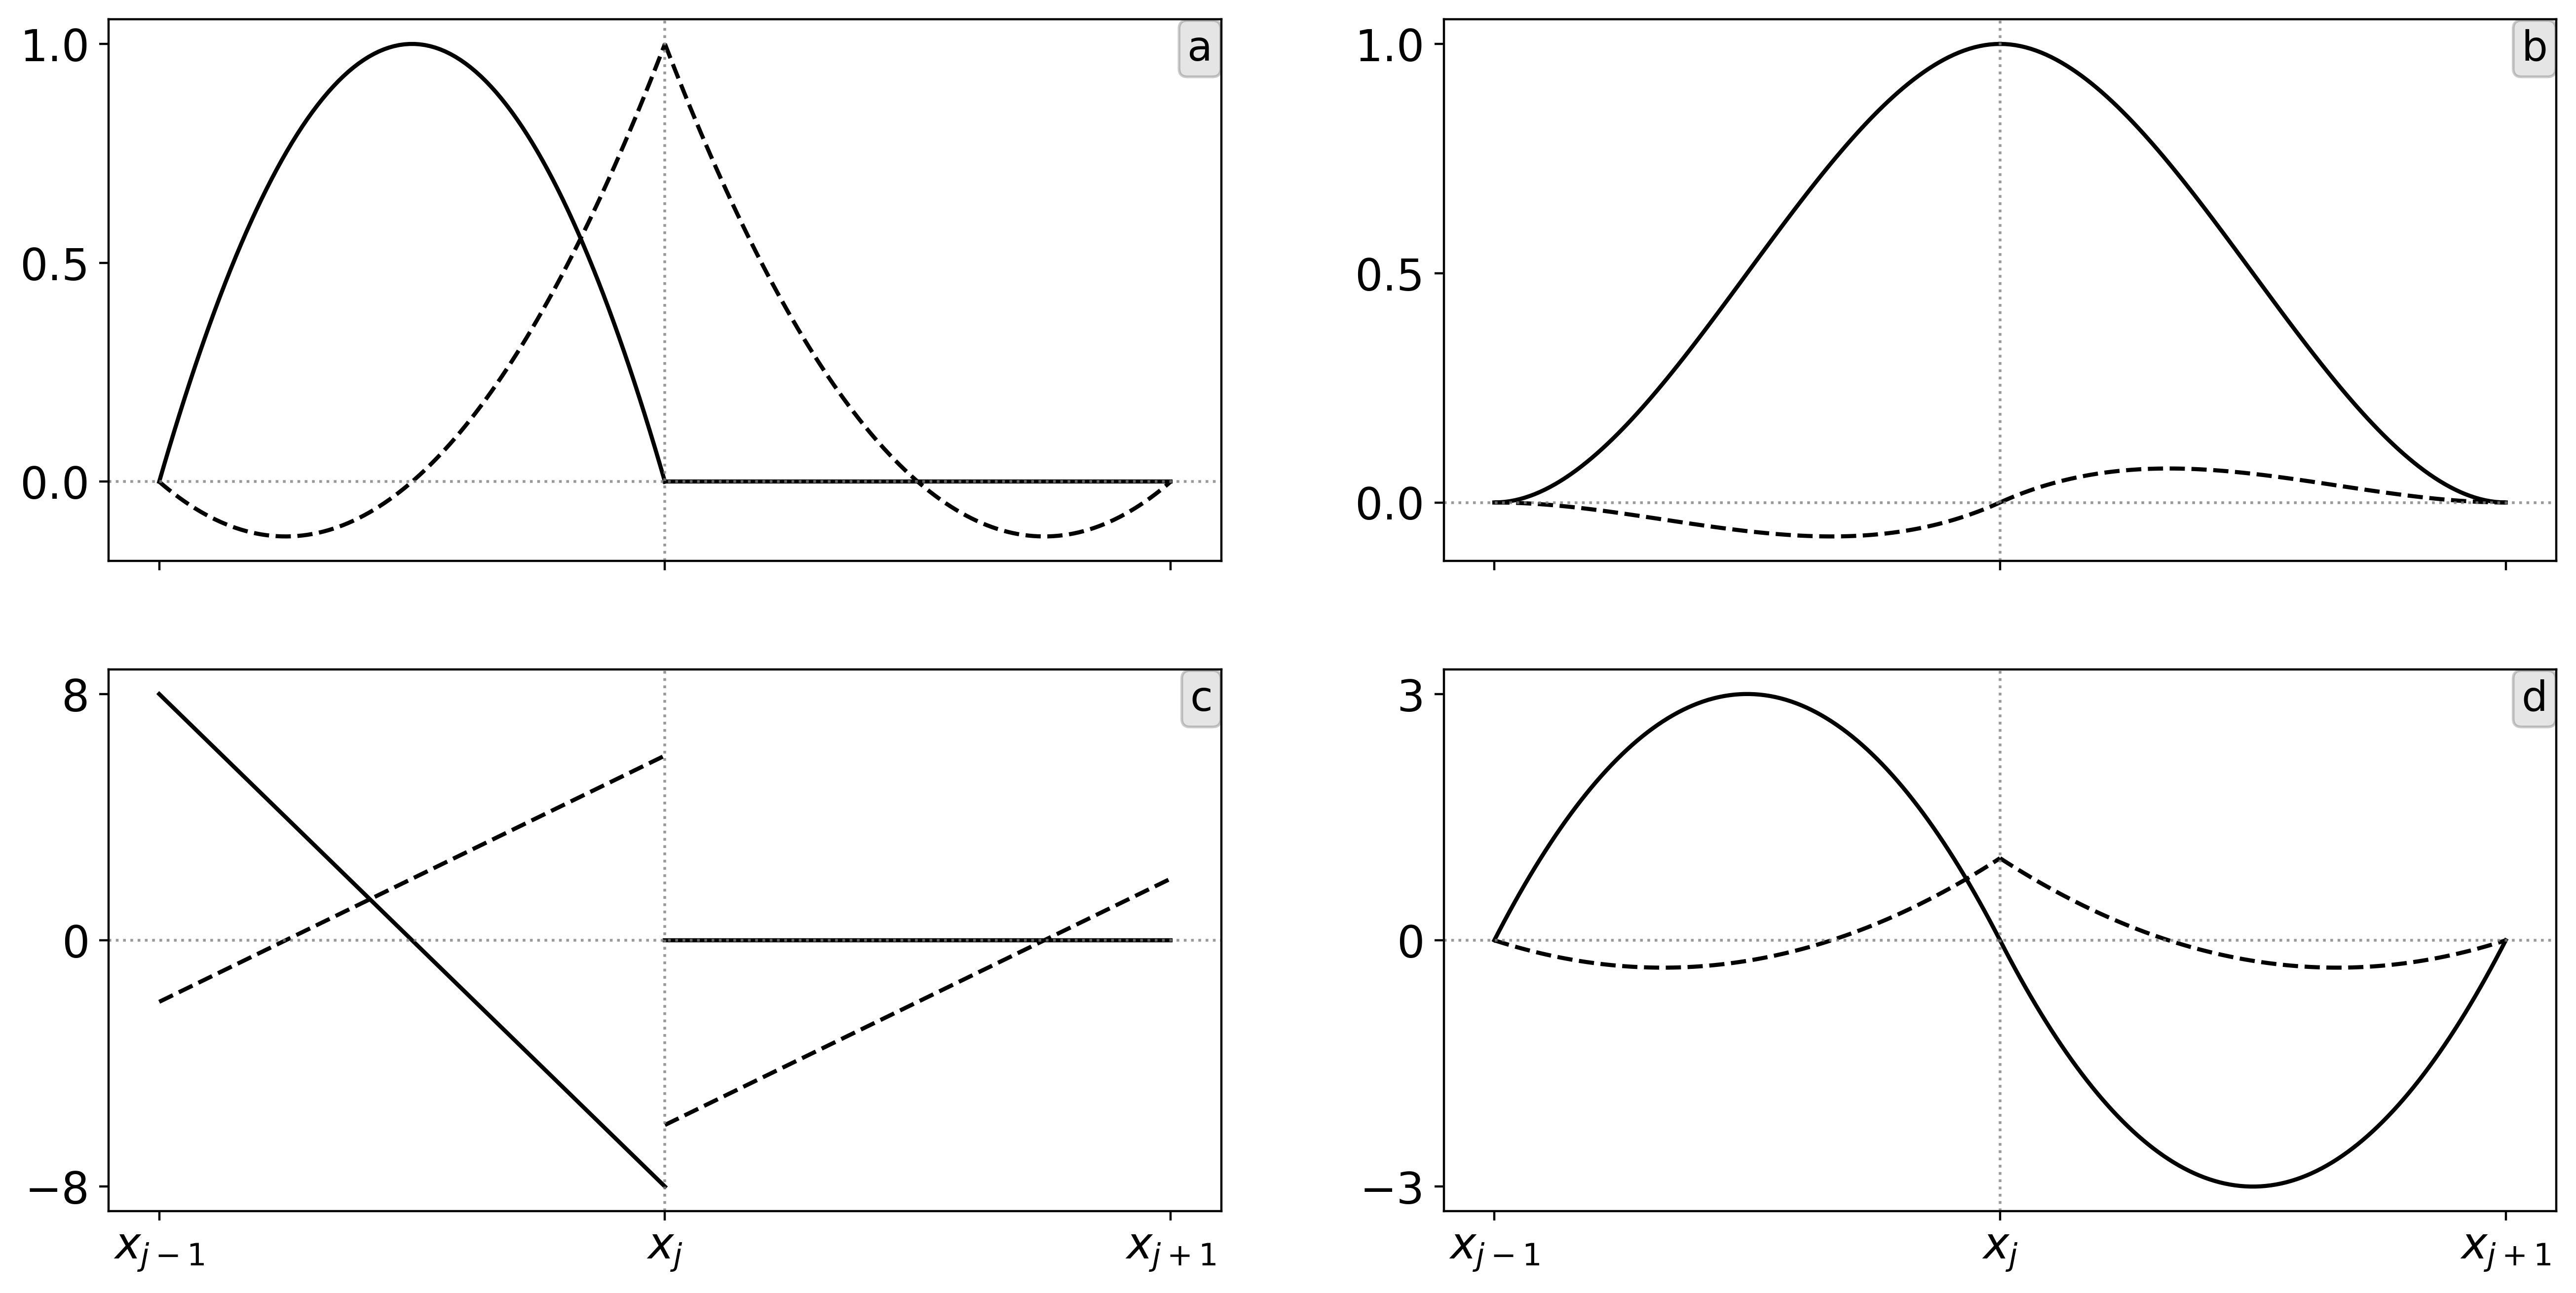
\includegraphics[width=\textwidth]{basisfunctions.png}
  \caption{
    The quadratic (\textbf{a}) and cubic (\textbf{b}) basis functions for the interval $[x_{j-1}, x_{j+1}]$ along with their derivatives (\textbf{c}) and (\textbf{d}), respectively. The solid lines denote $\{Q^1, C^1\}$, the dashed lines denote $\{Q^2, C^2\}$.
  }
  \label{fig: basisfunctions}
\end{figure}

We now proceed by rewriting our original set of equations \eqref{eq: full_continuity}--\eqref{eq: full_induction3} into weak Galerkin form. Each of the eight equations is multiplied by an appropriate element of the chosen basis (weight function), denoted by $h_j$, and integrate over the relevant domain. Because there are eight unknowns in our eigenvalue system, together with two basis functions and $N$ subdomains, this implies that the final matrix eigenvalue problem will have $16 N$ equations, resulting in a $16N \times 16N$ matrix. By extension, it becomes clear that using basis functions of even higher order will increase the size of this eigensystem considerably.

As an example we can write a part of the momentum-1 equation in weak Galerkin form. Because it is one of the simpler expressions and excellent as a short example, we consider the $T_1$ component on the right-hand side of Equation \eqref{eq: full_momentum1}, that is,
\begin{equation}
  \omega \rho_0 v_1 = \eps \left(\frac{\rho_0 T_1}{\eps}\right)'.
\end{equation}
These particular terms correspond to element $(2, 5)$ in the matrices. This ``number'' links to the indices of the state vector $\statevec$, because the momentum-1 equation is associated with $v_1$, or index $2$ in the state vector \eqref{eq: statevector}, and the $T_1$ component is associated with index $5$. As explained earlier we multiply the above equation with a weight function, and since we are using the Galerkin form this weight function is equal to the basis function, in this case the one associated with $v_1$ (i.e. a cubic polynomial), with notation $\hj{2}$. In the finite element representation adopted here, the $(v_1, T_1)$ contribution can be written as
\begin{equation} \label{eq: example_rho1_T1}
  \sum_{j=0}^N\omega \int \rho_0 \hj{2}\hk{2}du_1 =
  \sum_{j=0}^N\int \eps \hj{2}\left(\frac{\rho_0}{\eps}\hk{5}\right)'du_1,
\end{equation}
The $u_1$ dependence of the equilibrium density $\rho_0$ and basis functions $h^2$ and $h^5$ is implied. In this case, $h^2$ is cubic, because $v_1$ is associated with a cubic basis function; analogously $h^5$ is quadratic ($T_1$). The integrals are called \emph{matrix elements}, since the indices translate to the actual position in the final matrices of the eigenvalue problem. We will discuss this a little further in this section.

The matrix element corresponding to the left-hand side of Equation \eqref{eq: example_rho1_T1} can therefore be written as
\begin{equation}
  \bmat_{jk}(2, 2) = \int \rho_0 \hj{2}\hk{2}du_1,
\end{equation}
For the other side of the equal sign we can write the matrix element as
\begin{equation} \label{eq: amat_rho1_T1}
  \begin{aligned}
    \amat_{jk}(2, 5) &=
      \int \eps \hj{2}\left(\frac{\rho_0}{\eps}\hk{5}\right)'du_1, \\
      &\qquad \begin{cases}
        \text{u} = \eps\hj{2} \rightarrow \text{du} = \left(\eps'\hj{2} + \eps\dhj{2}\right)\text{d}u_1 \\
        \text{dv} = \left(\dfrac{\rho_0}{\eps}\hk{5}\right)'\text{d}u_1
          \rightarrow \text{v} = \dfrac{\rho_0}{\eps}\hk{5}
      \end{cases} \\
      &= \rho_0 \hj{2}\hk{5}\Bigr|_{\partial \Omega}
        - \int \frac{\eps'}{\eps}\rho_0 \hj{2}\hk{5}du_1
        - \int \rho_0 \dhj{2}\hk{5}du_1,
  \end{aligned}
\end{equation}
where we applied integration by parts using the standard notation ``u'' and ``v'' to denote the parts, and the first term has to be evaluated at the edges of the domain, annotated by $\partial\Omega$.

The same strategy is applied to all equations in the linear system, from which it follows that $\bmat$ will only have equal-number matrix elements (i.e. only $(1, 1)$, $(2, 2)$, etc.), implying that $\bmat$ is fully symmetric and real. The $\amat$-matrix on the other hand, will have cross-term elements such that it is, in general, not symmetric. Furthermore, $\amat$ might be complex, depending on the included physical effects. Terms that contain derivatives of the state vector components, as for example $(v_1, T_1)$, are integrated by parts.

\subsubsection{Integrals through Gaussian quadrature}
When all the matrix elements have been calculated and the entire system is rewritten in the weak Galerkin form, then all elements of course contain one or more integrals that still have to be calculated. This is the next ``obstacle'' in our mathematical treatment: because the coefficient functions are in general quite complicated expressions depending on $u_1$ we have to suppose that the solutions of those integrals are not known, and can only be calculated analytically for very simple equilibrium expressions. A naive first idea could be to make use of Riemann sums, where we approximate a given integral by a finite sum of small regions, and for sufficiently small partitions (i.e. a large number of summation terms), this sum will asymptotically converge to the actual solution. However, we are dealing with \emph{a lot} of integrals, the number of which strongly scales with the finite element domain discretisation. While Riemann sums may sound like a good idea, they are quite cumbersome, slow, and will probably have a major performance impact on the assembly of the matrices.

A much better idea would be Gaussian quadrature, which essentially approximates the integral with a sum as well, but instead of area partitions it relies on Gaussian weights and nodes originating from the roots of the n-th degree Legendre polynomial; this allows for an \emph{exact} integration of degree $2n - 1$ polynomials \citep{book_MHD}. Additionally, it uses far fewer nodes compared to Riemann sums and is hence much more efficient both in terms of accuracy and calculations needed to achieve a solution due to a clever choice of weighting scheme. As Gaussian quadrature formalisms can be found in any standard textbook on numerical analysis, we will not go into much detail regarding the mathematical background and convergence properties. {\legolas} uses a four-point Gaussian quadrature to numerically approximate the integrals, and as such an integral in the interval $[x_{j-1}, x_j]$ can be expressed as
\begin{equation}
  \int_{x_{j-1}}^{x_j} f(u_1)du_1 \approx
    \frac{1}{2}\left(x_j - x_{j-1}\right)\sum_{i=1}^4 w_i f\left(
     \frac{1}{2}\left(x_j - x_{j-1}\right)\xi_i + \frac{1}{2}\left(x_{j-1} + x_j\right)
    \right),
\end{equation}
where $\xi_i$ and $w_i$ are the evaluation points (nodes) and weights of the 4-point Gaussian quadrature, given by
\begin{equation} \label{eq: gaussian_nodes}
  \begin{aligned}
    \left(\xi_i, w_i\right) &= \left(
      \pm \sqrt{\frac{3}{7} - \frac{2}{7}\sqrt{\frac{6}{5}}}, \frac{18 + \sqrt{30}}{36}
    \right)
    \approx (\pm 0.339981, 0.652145), \\
    \left(\xi_i, w_i\right) &= \left(
      \pm \sqrt{\frac{3}{7} + \frac{2}{7}\sqrt{\frac{6}{5}}}, \frac{18 - \sqrt{30}}{36}
    \right)
    \approx (\pm 0.861136, 0.347854).
  \end{aligned}
\end{equation}
The function $f$ denotes the integral coefficients, which are essentially the equilibrium quantities and basis functions evaluated in the various evaluation points.

\section{Assembly of the system}
Armed with the MHD equations in weak Galerkin form and detailed knowledge on the finite element treatment and how to approach the integrals, all that is left is putting the pieces together into a consistent formalism. The main goal here is to eventually obtain an eigenvalue problem in which both matrices purely consist of numbers, such that they can be passed on to various linear algebra solvers. At this point we have all matrix elements calculated, such that there are three steps remaining in the formalism:
\begin{itemize}
  \item[i)] \textbf{Matrix assembly}: Translate the matrix elements into actual positions within the matrices and evaluate the various integrals at the same time, thereby assembling the actual matrices $\amat$ and $\bmat$. Special attention must be given to how the finite element representation, matrix elements and locations in the matrices are interconnected.
  \item[ii)] \textbf{Boundary conditions}: We still have to specify proper boundary conditions and take care of the surface terms introduced through integration by parts.
  \item[iii)] \textbf{Eigenfunction assembly}: When the eigenvalue problem is solved, the eigenvectors are obtained within the finite element formalism and still have to be transformed to ``proper'' eigenfunctions.
\end{itemize}

\subsubsection{Matrix assembly}
The actual assembly of both matrices $\amat$ and $\bmat$ in {\legolas} is done by sequential iteration over the grid points. From Equations \eqref{eq: basisfunction_Q1}--\eqref{eq: basisfunction_C2}, we see that the finite elements have a localised nature around every grid point $j$, meaning that only the elements associated with a certain region (that is, the grid point $j$ itself and its neighbours $j - 1$ and $j + 1$) yield a nonzero contribution. However, it is actually easier implementation-wise to loop over the elements in the interval $[x_{j-1}, x_j]$ instead of over those in $[x_{j-1}, x_{j+1}]$, because then the actual integration of the matrix elements can be done in the same way, independent of whether the basis functions are cubic or quadratic. If only the interval $[x_{j-1}, x_j]$ is considered, we end up with 16 possible combinations of the basis functions for every grid point. This translates into a $4 \times 4$ submatrix for every variable, where every one of the 16 elements corresponds to one specific combination of the shape functions. As there are eight variables in the state vector, this implies a $32 \times 32$ matrix block for every grid point, hereafter dubbed a ``quadblock'' as it consists of four $16 \times 16$ blocks (hereafter called ``subblocks''). Every one of those subblocks inside a quadblock corresponds to a quarter section of the aforementioned submatrix, which is a $2 \times 2$ block in every subblock. Hence, to recap, a $2 \times 2$ block times eight variables represents a $16 \times 16$ subblock, of which four combined form a $32 \times 32$ quadblock for every grid point. Note that for the case of self-gravity we have nine equations, hence an $18 \times 18$ subblock and a $36 \times 36$ quadblock.

The Gaussian quadrature used to numerically approximate the integrals actually implies that every grid interval
$[x_{j-1}, x_j]$ is subdivided into four points, meaning that the equilibrium expressions are probed using $4(N - 1)$ points rather than $N$ points. The way the matrices are then assembled is thus done on a double-loop basis, where the outer loop iterates over the intervals $[x_{j-1}, x_j]$ and the inner loop iterates over the four Gaussian nodes. This inner loop calculates the basis functions and matrix elements at every point, then multiplies the coefficients with the Gaussian weights and finally adds them all together in a consistent manner. Because every quadblock corresponds to the interval $[x_{j-1}, x_j]$, we still have to account for the contribution of the $x_{j+1}$ grid point. This is done by partially overlapping the quadblock in the next grid point with the one from the previous grid point.

Figure \ref{fig: matrix_assembly} shows a visual representation of the structure and assembly process for the $\amat$-matrix, only six grid points were used for the purpose of illustration. Panel a shows the general matrix, highlighting the block-tridiagonal structure. The dashed grey lines denote the $32 \times 32$ quadblocks of the matrix, and every dot represents a nonzero value. In total, five quadblocks can be distinguished for six grid points, one for every grid interval. Panel b shows a zoom-in of the quadblock corresponding to the second grid interval as annotated on the left panel, where it can be seen that the top-left corner of this quadblock overlaps with the bottom-right corner of the previous quadblock corresponding to the first grid interval. A single quadblock is further divided into four subblocks, with the location of the different state variables annotated on Panel c of Figure \ref{fig: matrix_assembly}.
The matrix element $\amat(2, 5)$ is highlighted in every subblock, which corresponds to the $(v_1, T_1)$ contribution, which are cubic $(v_1)$ and quadratic $(T_1)$ variables. The $2 \times 2$ blocks in the top-left corner of the quadblock corresponds to the top-left $2 \times 2$ corner of the right panel, as indicated by the background colours. Panel c shows the various (16) combinations of the regular basis functions for a (cubic, quadratic) contribution, where the blue curve corresponds to the cubic basis functions and the orange curves to the quadratic ones. It should be noted that Panel c only shows one specific case, that is, the regular $\hj{2}\hk{5}$ terms of the matrix element. If, for example, the $\hj{2}\hk{7}$ element is calculated (which would be an $a_2$ term in the momentum-1 equation), the quadratic basis functions have to be replaced by their cubic counterparts, because $a_2$ is also a cubic variable. A similar reasoning can be made for the other matrix elements. \vfill

\begin{figure}[t!]
  \centering
  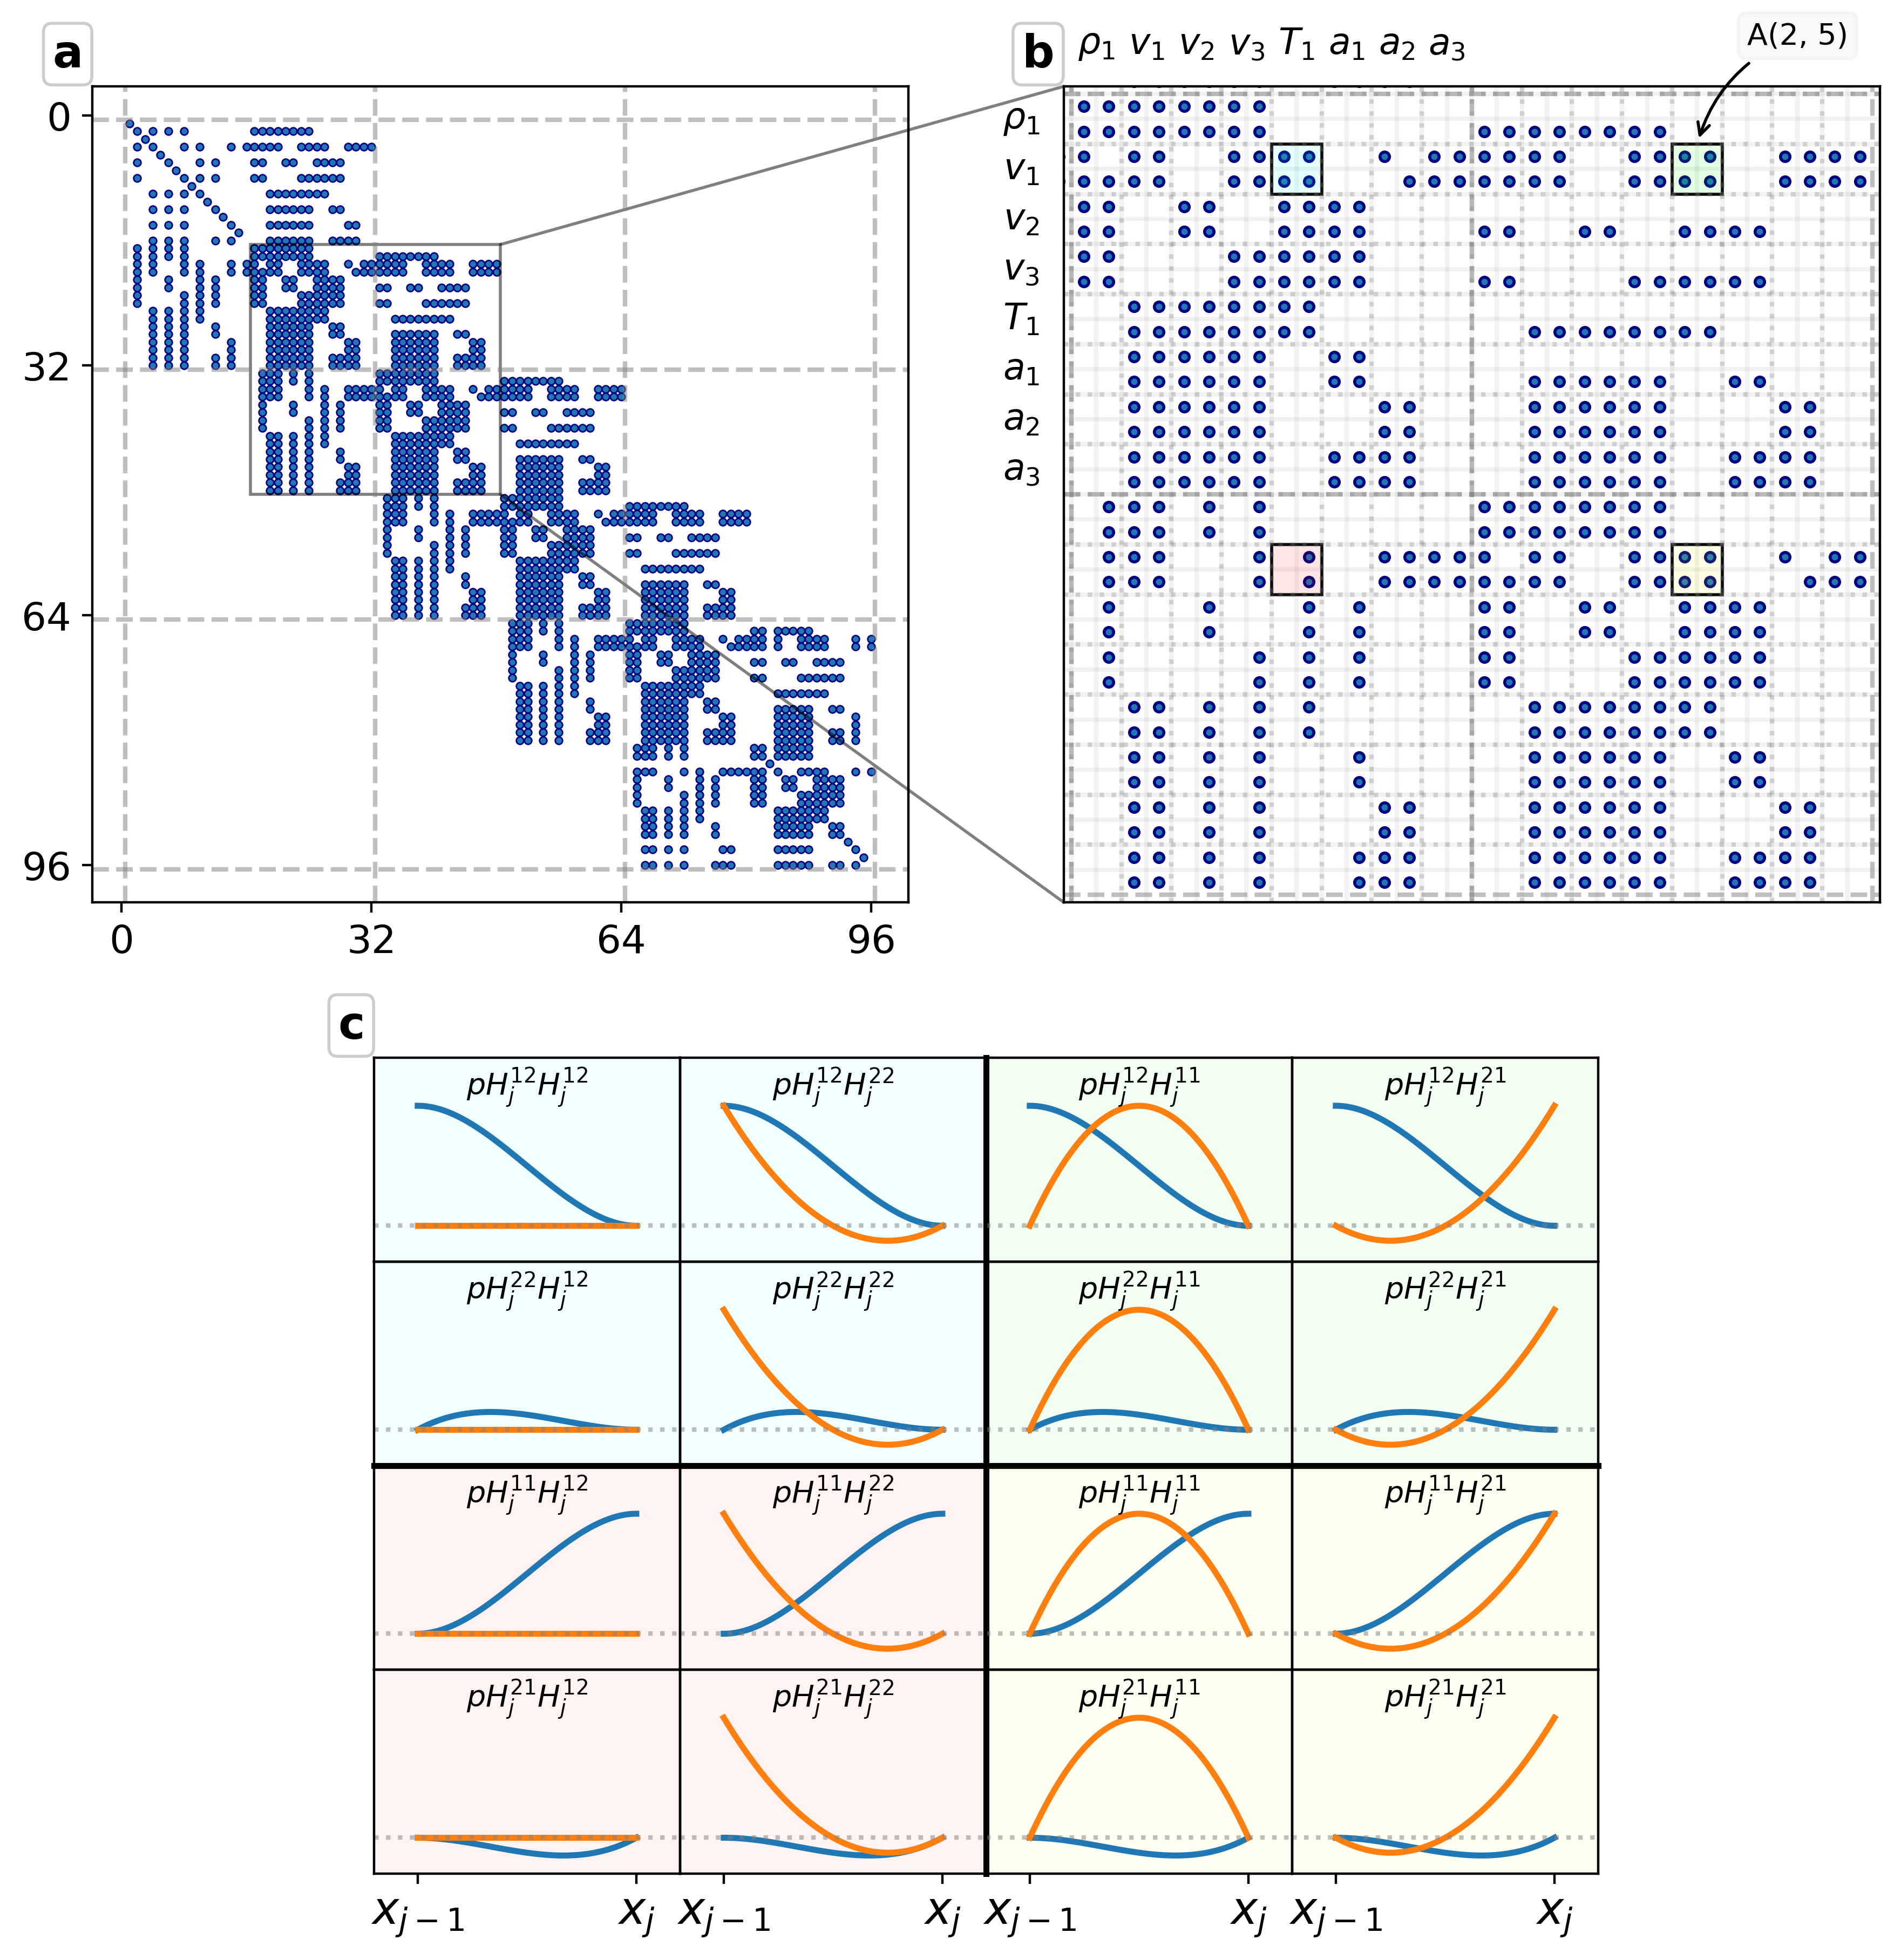
\includegraphics[width=\textwidth]{matrix_assembly.png}
  \caption{
    General assembly and structure of the finite element (complex) $\amat$ matrix. Panel \textbf{a}: example of a full matrix for six grid points, showing the block-tridiagonal structure where dots represent nonzero values. Panel \textbf{b} zooms in on one quadblock, showing the dependence of the different subblock positions with respect to the variables. The $2 \times 2$ blocks corresponding to (cubic, quadratic) element $(2, 5)$ are highlighted.
    Panel \textbf{c}: $2 \times 2$ block assembly for a general regular (cubic, quadratic) matrix element. Cubic elements are shown in blue, quadratic ones in orange. The dotted gray line denotes zero.
  }
  \label{fig: matrix_assembly}
\end{figure}

The term $pH_j^{\alpha\beta}H_j^{\alpha\beta}$ at the top of every subpanel on Panel c denotes which combination of the basis functions should be used, where $p$ stands for the integral coefficients. The exponent $\alpha\beta$ refers to the expressions for the basis functions, where $\alpha = 1$ stands for $Q_j^1$ or $C_j^1$, that is, Equations \eqref{eq: basisfunction_Q1} and \eqref{eq: basisfunction_C1}; while $\alpha = 2$ stands for $Q_j^2$ or $C_j^2$, hence Equations \eqref{eq: basisfunction_Q2} and \eqref{eq: basisfunction_C2}, depending on the variable under consideration (quadratic or cubic). The parameter $\beta$ stands for which part of the basis function should be taken: $\beta = 1$ means the first equation in cases, while $\beta = 2$ means the second one. As an example, we can look at $H_j^{12}H_j^{21}$: because $\amat(2, 5)$ represents a cubic and quadratic variable, this translates into $C_j^{12}Q_j^{21}$. For the cubic part, we therefore take the second equation of $C_j^1$, corresponding to $x_j \leq x \leq x_{j + 1}$. The quadratic part on the other hand is given by $Q_j^{21}$, which means that we take the first equation of $Q_j^2$, corresponding to $x_{j-1} \leq x \leq x_j$. This process is repeated for all matrix elements.

{\legolas} implements ``matrix splitting'', which means that every physical contribution is treated as a separate matrix. This is mainly done for numerical reasons: the code will simply avoid calculating matrix elements corresponding to physical terms that were disabled, thereby avoiding unnecessary calculations. As every physical contribution has its own matrix, the eigenvalue problem can be written as
\begin{equation} \label{eq: matrix_splitting}
	\omega \Bigl[
	\underbrace{\bmat}_{\substack{\text{\tiny regular} \\ \text{\tiny terms}}}
	+ \underbrace{\bmathall}_{\substack{\text{\tiny Hall} \\ \text{\tiny terms}}}
	\Bigr]\statevec
	= \Bigl[
		\underbrace{\amat}_{\substack{\text{\tiny regular} \\ \text{\tiny terms}}}
		+ \underbrace{\flowmat}_{\substack{\text{\tiny flow} \\ \text{\tiny terms}}}
		+ \underbrace{\etamat}_{\substack{\text{\tiny resistive} \\ \text{\tiny terms}}}
		+ \underbrace{\viscmat}_{\substack{\text{\tiny viscous} \\ \text{\tiny terms}}}
		+ \underbrace{\coolmat}_{\substack{\text{\tiny cooling} \\ \text{\tiny terms}}}
		+ \underbrace{\condmat}_{\substack{\text{\tiny conductive} \\ \text{\tiny terms}}}
		+ \underbrace{\hallmat}_{\substack{\text{\tiny Hall} \\ \text{\tiny terms}}}
	\Bigr]\statevec,
\end{equation}
but for all intents and purposes we will simply call the left- and right-hand side of this equation the $\bmat$ and $\amat$-matrices, respectively.


\subsubsection{Boundary conditions}
The system of differential Equations \eqref{eq: full_continuity}--\eqref{eq: full_induction3} still has to be complemented by a set of appropriate boundary conditions on both sides of the domain. For a Cartesian geometry, we look at a domain enclosed by two conducting walls. Clearly, the velocity component perpendicular to the walls has to be zero because there cannot be any propagation into a solid boundary. Mathematically, this translates into $\bv \cdot \unit{n} = 0$, where $\unit{n}$ represents the normal vector to the wall. Following the same reasoning, we also require that $\bb \cdot \unit{n} = 0$, so in terms of a vector potential, this implies $\unit{n} \times \ba = 0$. Hence, applying this to the set of linearised equations means that for the Cartesian case $v_1, a_2$, and $a_3$, all have to be zero on the boundaries. Furthermore, because we are dealing with a perfectly conducting wall, one has to take care when thermal conduction is included. In that case, the rigid wall directly influences the temperature because it acts as an energy reservoir essentially eliminating the temperature perturbation. Hence, if and only if perpendicular thermal conduction is taken into account, we have to supplement the boundary conditions by an additional conditions $T_1 = 0$ at the boundary. In theory there is a second possibility, which is treating the wall as a perfect insulator instead of a perfect conductor. In that case, there is no heat flux, which translates to the boundary condition $T_1' = 0$ instead of $T_1 = 0$. For now, we only consider the latter condition, that is, the one corresponding to a perfectly conducting wall.

In cylindrical geometry, we have the exact same boundary conditions as for the Cartesian case at the outer wall $r = R$, or at the outer edge of the accretion disk at $R$. The same is true at the inner disk edge, but for a flux tube extending to $r = 0$ we have to take the regularity conditions into account when treating the cylinder axis $r = 0$, which comes down to the fact that $r v_r$ should go to zero when approaching $r = 0$. Looking back at the transformations \eqref{eq: transformation} we applied, it follows that this condition is equivalent to $\widetilde{v_1} = 0$. Analogously, the same holds true for $a_2$ and $a_3$ such that these conditions are identical to the ones we applied for the Cartesian case, which is quite convenient implementation-wise. We again have to consider an additional condition if perpendicular thermal conduction is taken into account, because then $r T_1 = 0$ should also hold on the cylinder axis, which, similar to $v_1$, translates into $\widetilde{T_1} = 0$ at $r = 0$.

In the case of confinement by a perfectly conducting wall, we thus have straightforward boundary conditions, that is, $v_1 = 0, a_2 = 0, a_3 = 0$, and $T_1 = 0$ for both the Cartesian and cylindrical geometries on both sides (dropping the tildes). The latter boundary condition should only be taken into account if and only if perpendicular thermal conduction is included. These conditions are called \emph{essential boundary conditions}, meaning they \emph{have} to be satisfied by the system and should thus be explicitly handled.

\paragraph{Natural boundary conditions}
The integration by parts resulting from the weak Galerkin formulation gives rise to additional surface terms, which should also be evaluated at the boundaries. These kinds of conditions are called \emph{natural boundary conditions}, as they emerge in a natural way by reducing second-order derivatives to first-order derivatives when rewriting the eigenvalue problem. For simplicity we consider $B_{01} = v_{01} = 0$. In this case the additional surface terms for the momentum equation can be written as

\begin{equation} \label{eq: natural_boundary_v1}
  \begin{aligned}
    S_{v_1} &= \left[
      T_0 \hj{2}\hk{1}
      + \rho_0\hj{2}\hk{5}
      - \eps \Gmin \hj{2}\hk{6}
      + B_{03}\hj{2}\dhk{7}
      - \eps B_{02}\hj{2}\dhk{8}
    \right]_{\partial \Omega} \\
    &= v_1 \Bigl[
      T_0 \rho_1
      + \rho_0 T_1
      - \eps \Gmin a_1
      + B_{03}a_2'
      - \eps B_{02}a_3'
    \Bigr]_{\partial \Omega},
  \end{aligned}
\end{equation}
where the number in the superscript on $h_{j/k}$ denotes the index of the variable in the state vector $\statevec$.
The subscript $\partial \Omega$ means that these terms should be evaluated at the left or inner edge, as well as at the right or outer edge. In a similar manner, the surface terms for the energy and induction equations are given by
\begin{equation} \label{eq: natural_boundary_T1}
  \begin{aligned}
    S_{T_1} &= \icomplex \gmone T_1\Biggl[
      T_0'\dkappaperpdrho \rho_1
      + \left(T_0'\dkappaperpdT - \frac{\eps'}{\eps}\skappaperp{0}\right)T_1
      + \skappaperp{0}T_1'
    \Biggr. \\
    &+ 2\left(\eta_0 k_3 (\eps B_{02})' - \eta_0 k_2 B_{03}' - \eps T_0' \Gmin \dkappaperpdB\right)a_1 \\
    &+ 2\left(T_0' B_{03} \dkappaperpdB + \eta_0 B_{03}'\right)a_2'
     - 2\left(\eps B_{02}T_0'\dkappaperpdB + \eta_0 (\eps B_{02})'\right)a_3'
    \Biggr],
  \end{aligned}
\end{equation}

\begin{equation} \label{eq: natural_boundary_a2}
  S_{a_2} = \icomplex \eta_0 a_2 \bigl(a_2' - k_2 a_1\bigr),
\end{equation}

\begin{equation} \label{eq: natural_boundary_a3}
  S_{a_3} = \icomplex \eta_0 \eps a_3 \bigl(a_3' - k_3 a_1\bigr),
\end{equation}

which should all be evaluated at the boundaries. For the case of a solid wall, we see that the natural boundary conditions simplify considerably, because if $v_1, a_2$, and $a_3$ are all zero at the wall, then $S_{v_1}, S_{a_2}$ and $S_{a_3}$ are also zero and can be omitted. The natural boundary condition on $T_1$ is only relevant if resistivity or perpendicular thermal conduction is included. However, in the case of the latter, the additional essential boundary condition requires that $T_1 = 0$, in which case $S_{T_1}$ drops out as well. The only combination in which the surface terms for the energy equation are nonzero is when resistivity is included but perpendicular thermal conduction is omitted. In that case, the resistive heating terms should be included in the calculation, which is done by adding the appropriate terms to the matrix elements $\amat(5, 6)$, $\amat(5, 7)$ and $\amat(5, 8)$.

Currently, only fixed wall boundary conditions are implemented in {\legolas}. However, the surface terms described here can be used to impose other types of boundary conditions as well. In the case of a plasma-vacuum-wall transition, we have, for example, Bessel functions at the outer boundary of a cylindrical geometry \citep{book_roberts}, which encode the analytic vacuum solution for the electromagnetic field in the outer vacuum region. These expressions can then be used to rewrite the surface terms \eqref{eq: natural_boundary_v1}--\eqref{eq: natural_boundary_a3} in an appropriate way such that they can be added to their respective subblock positions in the matrix. This is one of the planned extensions to be included in future versions of {\legolas}.

\paragraph{Essential boundary condition}
The essential boundary conditions as described earlier have to be implemented explicitly. This is done by omitting the relevant basis functions that do not satisfy the boundary conditions on the edges. Consider as an example the variable $v_1$, which is associated with a cubic basis function. From Figure \ref{fig: basisfunctions}, we see that the only cubic element that is nonzero at the left boundary is $C_j^{12}$, which implies that the matrix elements where it appears should be zeroed out. Looking back at how the quadblock is composed in Figure \ref{fig: matrix_assembly}, the boundary condition $v_1 = 0$ corresponds to forcing the odd rows and columns of the $v_1$ contribution to zero, for subblocks $1, 2,$ and $3$ on the left boundary (that is, the first node $j$) because these correspond to the $2 \times 2$ blocks in blue, green and red on the right panel. Similarly, on the right side (viz. the last node $j$), only $C_j^{11}$ is nonzero, which implies that the odd rows and columns of subblocks $2, 3,$ and $4$ have to be zeroed out (corresponding to green, red, and yellow). Extending this reasoning to the essential boundary condition on $T_1$, we see that in this case the even rows and columns should be handled because $T_1$ is associated with a quadratic element. This is done for both matrices.

Of course, ``just'' zeroing out rows and columns in a matrix has the unpleasant side effect that the matrices become singular. For the $\amat$-matrix, this is not necessarily a problem; however, the $\bmat$ matrix is not allowed to be singular because it is inverted when solving the general eigenvalue problem using the QR-algorithm. Therefore, we introduce a one on $\bmat$'s diagonal at the location that was zeroed out, and an element $\delta$ on $\amat$'s diagonal. The effect of this is that one essentially ``forces'' the boundary condition, because this implies that $\delta x_j^i = \omega x_j^i$. By extension, if $\delta$ is taken to be a large number (we take $\delta = 10^{20}$), this means that $x_j^i = 0$ which corresponds to the essential boundary we want to impose. The only side effect of this approach is that it introduces eigenvalues equal to $\delta$. However, because $\delta$ is taken to be large, these will not influence the spectrum in any way, and they can be easily filtered out during postprocessing. This method thus provides a relatively easy and straightforward way to impose Dirichlet boundary conditions at the edges. The imposed boundary conditions are noticeable on Panel a of Figure \ref{fig: matrix_assembly}, especially for the first node. The odd rows and columns that were zeroed out can clearly be seen, together with the elements introduced on the main diagonal.

\subsubsection{Assembly of the eigenfunctions}
When solving the eigenvalue problem the eigenvectors associated with each eigenvalue are (optionally) calculated as well. These eigenvectors are obtained within the finite element formalism, and hence still need to be transformed to the actual eigenfunction representation. Since they are calculated along with the eigenvalues in the matrix eigenvalue problem, all eigenvectors have a similar structure as Figure \ref{fig: matrix_assembly}. One row of a $16 \times 16$ subblock in a single quadblock (and hence corresponding to one particular grid point) is shown in Figure \ref{fig: subblock_row}, and every eigenvector can be thought of as having $N$ of these rows next to each other. This implies that the information of all eight (in MHD) eigenfunctions is contained in the single eigenvector associated with that particular eigenvalue, hence every eigenfunction corresponds to a single specific set $\{k_2, k_3, \omega\}$.

\begin{figure}[t]
  \centering
  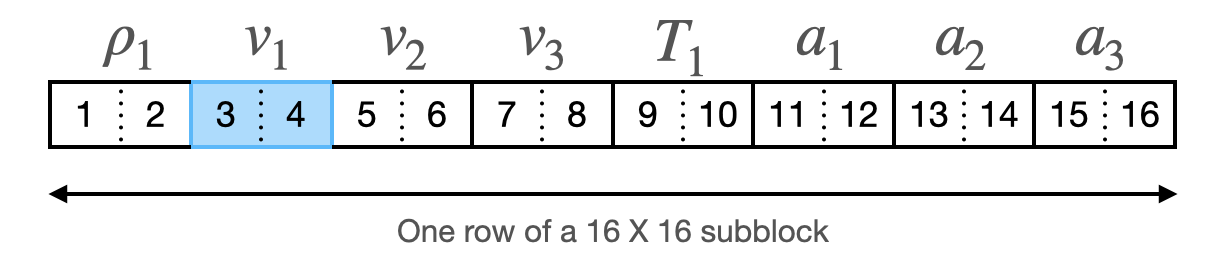
\includegraphics[width=\textwidth]{subblock_row.png}
  \caption{
    One row of a single subblock in a single quadblock, visualising (part of) the internal structure of an eigenvector. Every eigenvector has $N$ of these blocks.
  }
  \label{fig: subblock_row}
\end{figure}

Linking the structure in Figure \ref{fig: subblock_row} back to the layout of the matrix in Figure \ref{fig: matrix_assembly}, the $v_1$ eigenfunction, for example, can be assembled per grid point $j$ as
\begin{equation}
  v_{1, j} = E_{v, j}(3)C_j^{12} + E_{v, j}(4)C_j^{22} + E_{v, j}(3 + 16)C_j^{11} + E_{v, j}(4 + 16)C_j^{21},
\end{equation}
where $E_{v, j}$ indicates the eigenvector subblock corresponding to the $j$-th grid point; $C_j$ denotes the cubic basis functions since we are calculating the regular $v_1$ eigenfunction (which is a cubic variable). The indices in the eigenvector subblock correspond to 3, 4, 3 + 16 and 4 + 16, as we need $v_1$ and 16 is the size of the subblock. The basis functions are calculated using the position corresponding to the current grid point. In reality an eigenfunction has $2N - 1$ points for a grid of $N$ points, which is related to the fact that we overlay the bottom-right part of the previous quadblock with the top-left part of the current quadblock, per grid point; the minus one comes from no overlaying for the first quadblock. In the first grid point the eigenfunction is sampled on the left edge of the current interval; for all the following quadblocks the eigenfunction is sampled in the middle and right edge of the grid interval for every grid point. In the end the entire eigenfunction is assembled for every eigenvalue, taking into account the finite element representation and basis functions. The obtained eigenfunctions still have to be transformed back to ``regular'' values by undoing the transformation applied in Equation \eqref{eq: transformation}.

Similarly, we can calculate physical quantities of interest derived from the eigenfunctions. An example is the perturbed magnetic field $\bb_1 = \nabla \times \ba_1$, which can be constructed using the eigenfunctions of the vector potential as
\begin{equation}
  \bb_1 =
    \icomplex \left(\frac{k_2}{\eps}a_3 - k_3 a_2\right)\uunit{1}
    + \left(\icomplex k_3 a_1 - a_3'\right)\uunit{2}
    + \frac{1}{\eps}\left[\bigl(\eps a_2\bigr)' - \icomplex k_2 a_1 \right]\uunit{3},
\end{equation}
Due to the $\nabla$-operator present we also need the derivatives of the eigenfunctions, which can be assembled in a similar manner as the standard eigenfunctions but using the derivatives of the basis functions instead. Similarly, once we have $\bb_1$ we can also calculate its divergence and curl. Other quantities of interest may be the divergence and curl of the velocity perturbation, representing the compressibility and vorticity, respectively; or the entropy. Additionally, whenever we have a background magnetic field the perturbed vector quantities can be expressed in a reference frame with one component parallel and two components perpendicular to the field lines, which may also be of interest for certain use cases.

\cleardoublepage

\chapter{Legolas applications} \label{ch: legolas_applications}


\graphicspath{{05-applying_legolas/figures/}}

\begin{chapterquote}[Robert C. Martin][Clean Code: A Handbook of Agile Software Craftsmanship][]
  Why do most developers fear to make continuous changes to their code? Because they are afraid they'll break it.
  Why are they afraid they'll break it? Because they don't have tests.
\end{chapterquote}

\usespublishedwork{
  Most of this Chapter was published in ``Legolas: a novel tool for magnetohydrodynamic spectroscopy'', 2020, \apjs,
  251, 25 \citep{claes2020_legolas}. N. Claes developed {\legolas} in close collaboration with J. De Jonghe, generated the data and figures and wrote a first draft of the manuscript; J. De Jonghe revised and extended the manuscript. R. Keppens contributed to the revision of the paper.
}

In the previous Chapter we discussed the mathematical formalism behind {\legolas}. As is common practice when developing a brand new numerical code we now have to test the implementation against various known results. This Chapter will mostly be dedicated to the validation of our new numerical tool, by comparing numerical spectra with known results from theory and/or the literature. Additionally, we will briefly touch upon the extensive (and continuous) testing framework {\legolas} uses.

\section{Introduction}
Any piece of software, both existing and newly developed, should be accompanied by a decent testing framework to ensure that any changes made to the code, either in the present or in the future, do not break things that were previously working fine. It is easy to develop a piece of code, it is less easy to develop a \emph{working} piece of code, and finally it is certainly not enough for code to just ``work''. Every part of the implementation should be tested against known results in order to make sure that the code actually does what it is expected to do. In an ideal world, every single line of a code base is tested at least once, while at the same time also accounting for various branches in the logic.

In this Chapter we validate {\legolas} against a plethora of test cases, thereby ensuring a correct treatment of the governing equations. Depending on which physical effects are taken into account, we know a priori some general spectral properties that should hold, and we can thus test the properties of the obtained spectra against our predictions. For eigenmode quantifications of ideal, static MHD configurations under adiabatic conditions, we know that the static -- that is, no equilibrium flow -- and adiabatic linear MHD equations make the problem self-adjoint. When performing a standard Fourier analysis in the ignorable directions, the resulting eigenvalue problem is then Hermitian, meaning that all eigenfrequencies will be either fully real (stable waves) or fully complex (pure damped or unstable modes), hence they are found on the real or imaginary axis of the complex eigenfrequency plane, and the full MHD spectrum will be both left-right and up-down symmetric. The inclusion of nonideal effects like resistivity or thermal conduction lifts the self-adjointness of the eigenvalue problem, allowing the eigenmodes to move away from the axes into the complex plane, and the up-down symmetry gets broken. As long as the equilibrium configuration is static, all (adiabatic or non-adiabatic) modes will still have a complementary mode that lies mirrored around the imaginary axis, making the entire spectrum left-right symmetric. This is related to the forward and backward propagating mode symmetry, or the equivalent statement on the parity-time (PT) symmetry.

The inclusion of a background flow breaks the left-right symmetry of the MHD spectrum, resulting in an even more complicated spectral structure. However, the study of the ideal, linear MHD spectrum of flowing plasmas is still governed by a pair of self-adjoint operators \citep{goedbloed2011,book_MHD}, and it leaves the up-down symmetry of the spectrum intact (where every overstable mode has an equivalent damped counterpart at the same frequency).

The actual validation of the code should follow a stepwise approach, where we first test the most simple cases. This is dictated by common logic: if even the most simple cases do not work, then we can never expect correct spectra for more complicated equilibria. Hence to begin with, we discuss results for adiabatic equilibria where only gravity is included. In this case we can compare numerical spectra obtained through {\legolas} with analytical solutions acquired by solving dispersion relations; here, we first focus on stratified atmospheres containing $p$ and $g$ modes. We then move on to cylindrical geometries, where we first look at adiabatic flux tubes, followed by the inclusion of flow effects by considering equilibria known to be susceptible to KHI and Suydam cluster modes. Next, our focus shifts to nonadiabatic effects by looking at a resistive MHD calculation for a case without gravity, where the value of a quasi-mode is known analytically. Resistive tearing modes are also discussed, combining the effects of flow and resistivity. Finally we will treat the inclusion of thermal conduction and optically thin radiative cooling effects, where we look at nonadiabatic discrete Alfv\'en waves and magnetothermal modes. Validation of the various spectra is mostly done using a visual comparison with existing figures from literature, which is generally speaking sufficient as spectra are quite sensitive to even very minor changes in background conditions or matrix elements.


\section{Cartesian cases: waves in stratified atmospheres}
First of all we discuss multiple theoretical results for adiabatic equilibria in a Cartesian geometry, where only gravity is included. We consider $p$ and $g$ modes in stratified layers and pay special attention to specific unstable branches.

\subsection{Gravito-MHD waves} \label{ss: gravito-mhd}
The first test case covers gravito-MHD waves as discussed in \citet[Figure 7.9]{book_MHD}, which handles an exponentially stratified atmosphere with constant sound and Alfv\'en speeds. This magnetised atmosphere contains the generalisation of the $p$ and $g$ modes of an unmagnetised layer, and the constancy of the sound and Alfv\'en speed renders this particular configuration analytically tractable (even though it has an inhomogeneous density profile), because the slow and Alfv\'en continua collapse to points. the geometry is Cartesian with $x \in [0, 1]$ and an equilibrium configuration given by
\begin{equation} \label{eq: gravito_mhd}
  \begin{gathered}
    \rho_0 = \rho_c \exp\left(-\alpha x\right), \qquad p_0 = p_c \exp\left(-\alpha x\right), \\
    \bb_0 = B_c \exp\left(-\frac{1}{2}\alpha x\right)\unit{z}, \qquad \alpha = \frac{\rho_c g}{p_c + \frac{1}{2}B_c},
  \end{gathered}
\end{equation}
where $p_c$ and $B_c$ are taken to be 0.5 and 1, respectively, as to yield a plasma beta equal to unity. The parameter $\alpha$ is taken to be 20, which, together with $g = 20$, is used to constrain the value for the constant $\rho_c$. These four equations completely determine the equilibrium configuration, because the temperature is $T_0 = p_0/\rho_0$, following the ideal gas law. The spectrum discussed in \citet{book_MHD} is actually the solution to the analytic dispersion relation for gravito-MHD waves, which shows the squared eigenvalue as a function of wavenumber for a fixed angle $\theta = \pi / 4$ between the wave vector $\bk_0$ and the magnetic field $\bb_0$. However, the spectrum as calculated by {\legolas} corresponds to one single equilibrium configuration, meaning one value for $k_y$ and $k_z$. In order to reproduce Figure 7.9 from \citet{book_MHD} and compare the results, we performed 100 different runs where the equilibrium parameters in Equation \eqref{eq: gravito_mhd} remained unchanged, but $k_y$ and $k_z$ took on 100 different values between $0$ and $\sqrt{250}$ as to yield a wavenumber range for $k_0^2$ between 0 and 500. Because the magnetic field is purely aligned with the $z$-axis, we can write $\kpara = k_z = k_0\cos(\theta)$ and $\kperp = k_y = k_0\sin(\theta)$. All runs were performed using 351 gridpoints, yielding a matrix size of $5616 \times 5616$.

\begin{figure}[t]
  \centering
  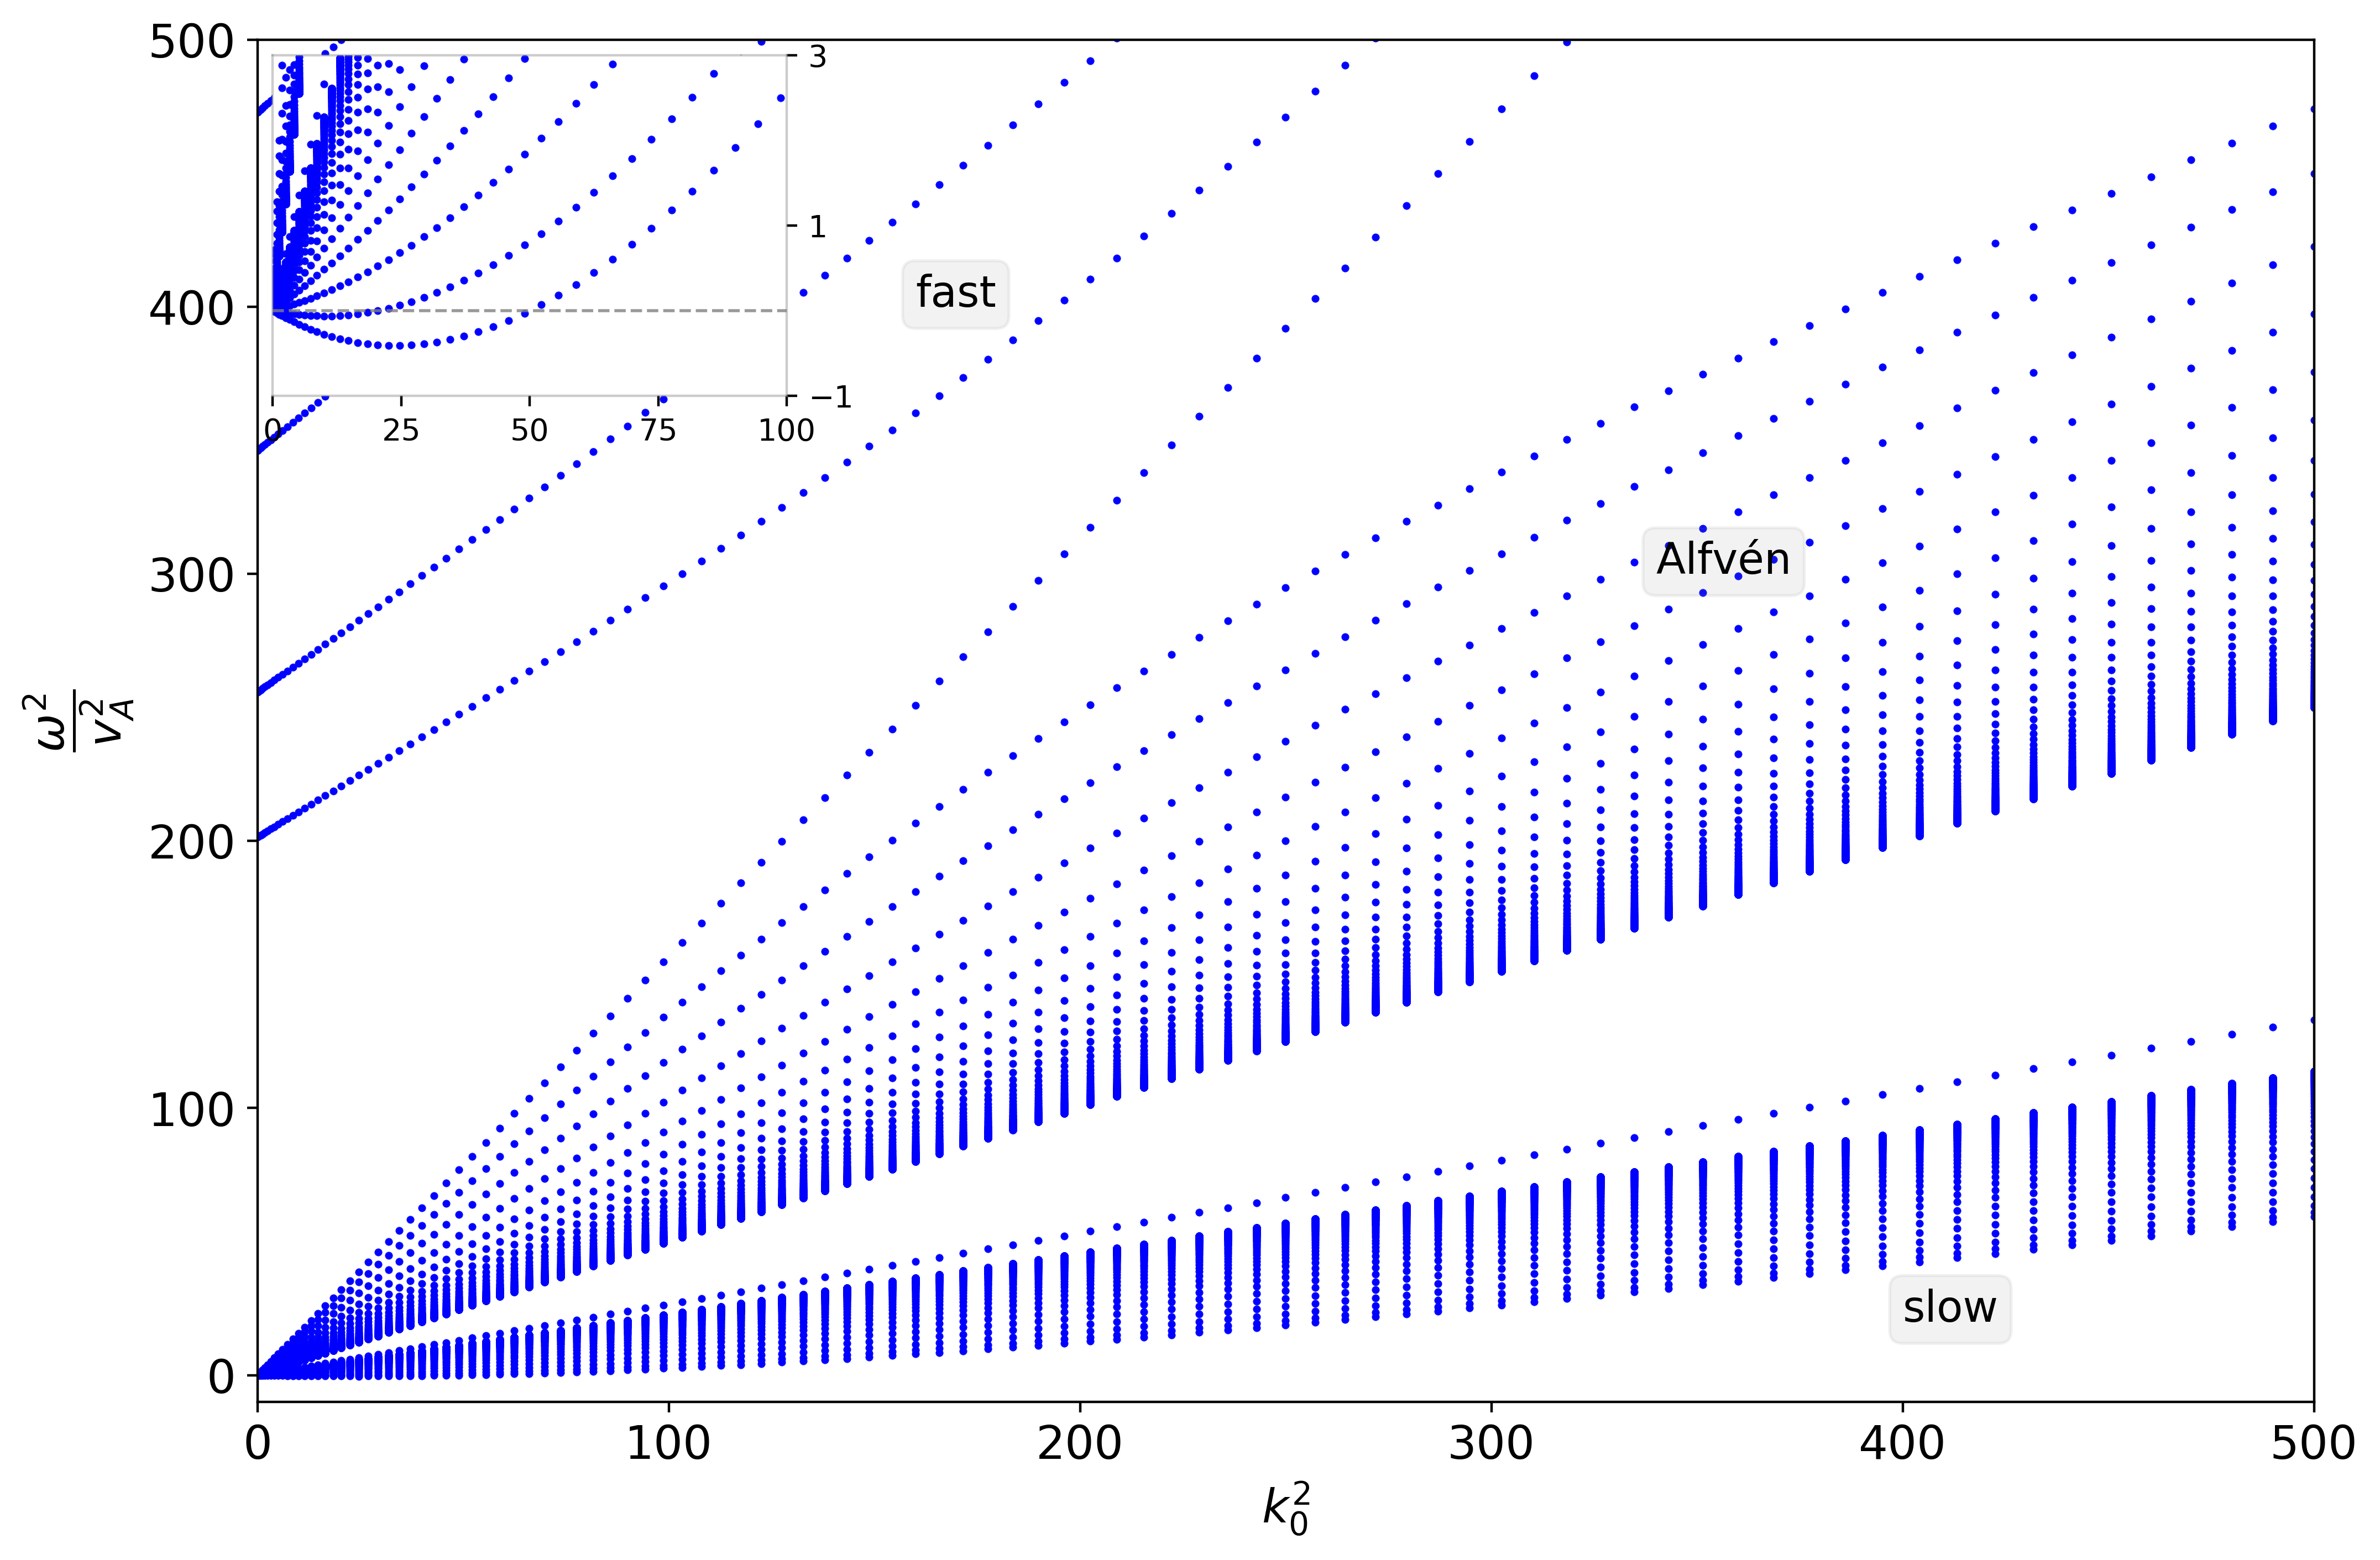
\includegraphics[width=\textwidth]{gravito_mhd.png}
  \caption{
    Spectrum of gravito-MHD modes, obtained through 100 {\legolas} runs of 351 gridpoints each. The fast (top), Alfv\'en (middle) and slow (bottom) branches of the MHD spectrum are clearly visible. The inset shows unstable slow modes at low frequencies.
  }
  \label{fig: gravito_mhd}
\end{figure}

The results are shown in Figure \ref{fig: gravito_mhd}, where every vertical collection of points at the same $k_0^2$ value represents one single {\legolas} run. Because we are in an MHD regime with a plasma $\beta = 1$, the three MHD subspectra can be clearly distinguished, showing the fast $p$ modes (top-left branches), Alfv\'en $g$ modes (middle branches), and slow $g$ modes (bottom branches). The inset shows a zoom-in near the marginal frequency of the spectrum, showing unstable $(\omega^2 < 0)$ slow MHD modes. These long-wavelength unstable modes are related to the Parker instabilities, due to magnetic buoyancy, as we will show in Section \ref{ss: quasi-parker}. Note that because this case is adiabatic and fully self-adjoint, every individual MHD spectrum is left-right and up-down symmetric in the complex eigenfrequency plane, but this aspect is hidden from the $\omega^2$ -- $k_0^2$ view shown here.


\subsection{Quasi-Parker instabilities} \label{ss: quasi-parker}
Next we discuss a modified case of the gravito-MHD waves, namely a spectrum showing quasi-Parker instabilities as done in \citet[Figure 12.2]{book_MHD}. The difference with the previous case is that a fully analytic description is no longer possible, because the introduction of magnetic shear leads to continuous ranges in the MHD spectrum. Instead of showing the spectrum for one single value for $\theta$, we now vary the direction of the wave vector $\bk_0$ between 0 and $\pi$. The equilibrium configuration is similar to the one in Section \ref{ss: gravito-mhd}, given in Cartesian geometry by
\begin{equation} \label{eq: quasi-parker}
  \begin{gathered}
    \rho_0 = \rho_c \exp\left(-\alpha x\right),
    \qquad
    p_0 = p_c \exp\left(-\alpha x\right),
    \qquad
    \alpha = \frac{\rho_c g}{p_c + \frac{1}{2}B_c}, \\
    B_{02} = B_c \exp\left(-\frac{1}{2}\right)\sin\left(\lambda x\right),
    \qquad
    B_{03} = B_c \exp\left(-\frac{1}{2}\right)\cos\left(\lambda x\right),
  \end{gathered}
\end{equation}
where magnetic shear was introduced through the parameter $\lambda$. The quantities $\alpha$ and $B_c$ are assigned the same values as in Equation \eqref{eq: gravito_mhd}; though now $g = 0.5$ and $p_c = 0.25$, which yield a plasma beta $\beta = 0.5$. The wave vectors are given by $k_y = \pi\sin(\theta)$ and $k_z = \pi\cos(\theta)$, such that $k_0^2 \approx 10$. The angle $\theta$ was varied between 0 and $\pi$ for a total of 100 runs at 351 grid points each, shown in Figure \ref{fig: quasi_parker}.

The left panels handle the case without magnetic shear, that is, $\lambda = 0$, which basically reduces to the one from the previous subsection. In this case, the slow and Alfv\'en continua collapse into single point values, denoted in red and cyan, respectively. The right panels show the same configuration where $\lambda = 0.3$ was taken, introducing magnetic shear, which introduces genuine continua seen as bands. These continua affect the overall stability and organise the entire MHD spectrum: all discrete modes are fully aware of the essential spectrum formed by these (slow and Alfv\'en) continua and the (fast) accumulation points at infinite frequency. All features of the original figure in \citet{book_MHD} are reproduced. The inset zooms into the region where both continua overlap, showing quasi-interchange and interchange instabilities. Once more, each run, shown here collectively in Figure \ref{fig: quasi_parker}, actually has a spectrum that is left-right and up-down symmetric in the eigenfrequency plane. This is depicted on Panels c and d, which show the eigenfrequency view for one single case $(\theta = 0.3\pi)$. The continuum ranges separate nicely: the collapsed single point values are denoted by cyan (Alfv\'en) and red (slow) points on Panel c, and the genuine continua are shown with cyan and red bands on Panel d. The instabilities themselves are situated on the (positive) imaginary axis, due to the self-adjointness of the eigenvalue problem.

\begin{figure}[t]
  \centering
  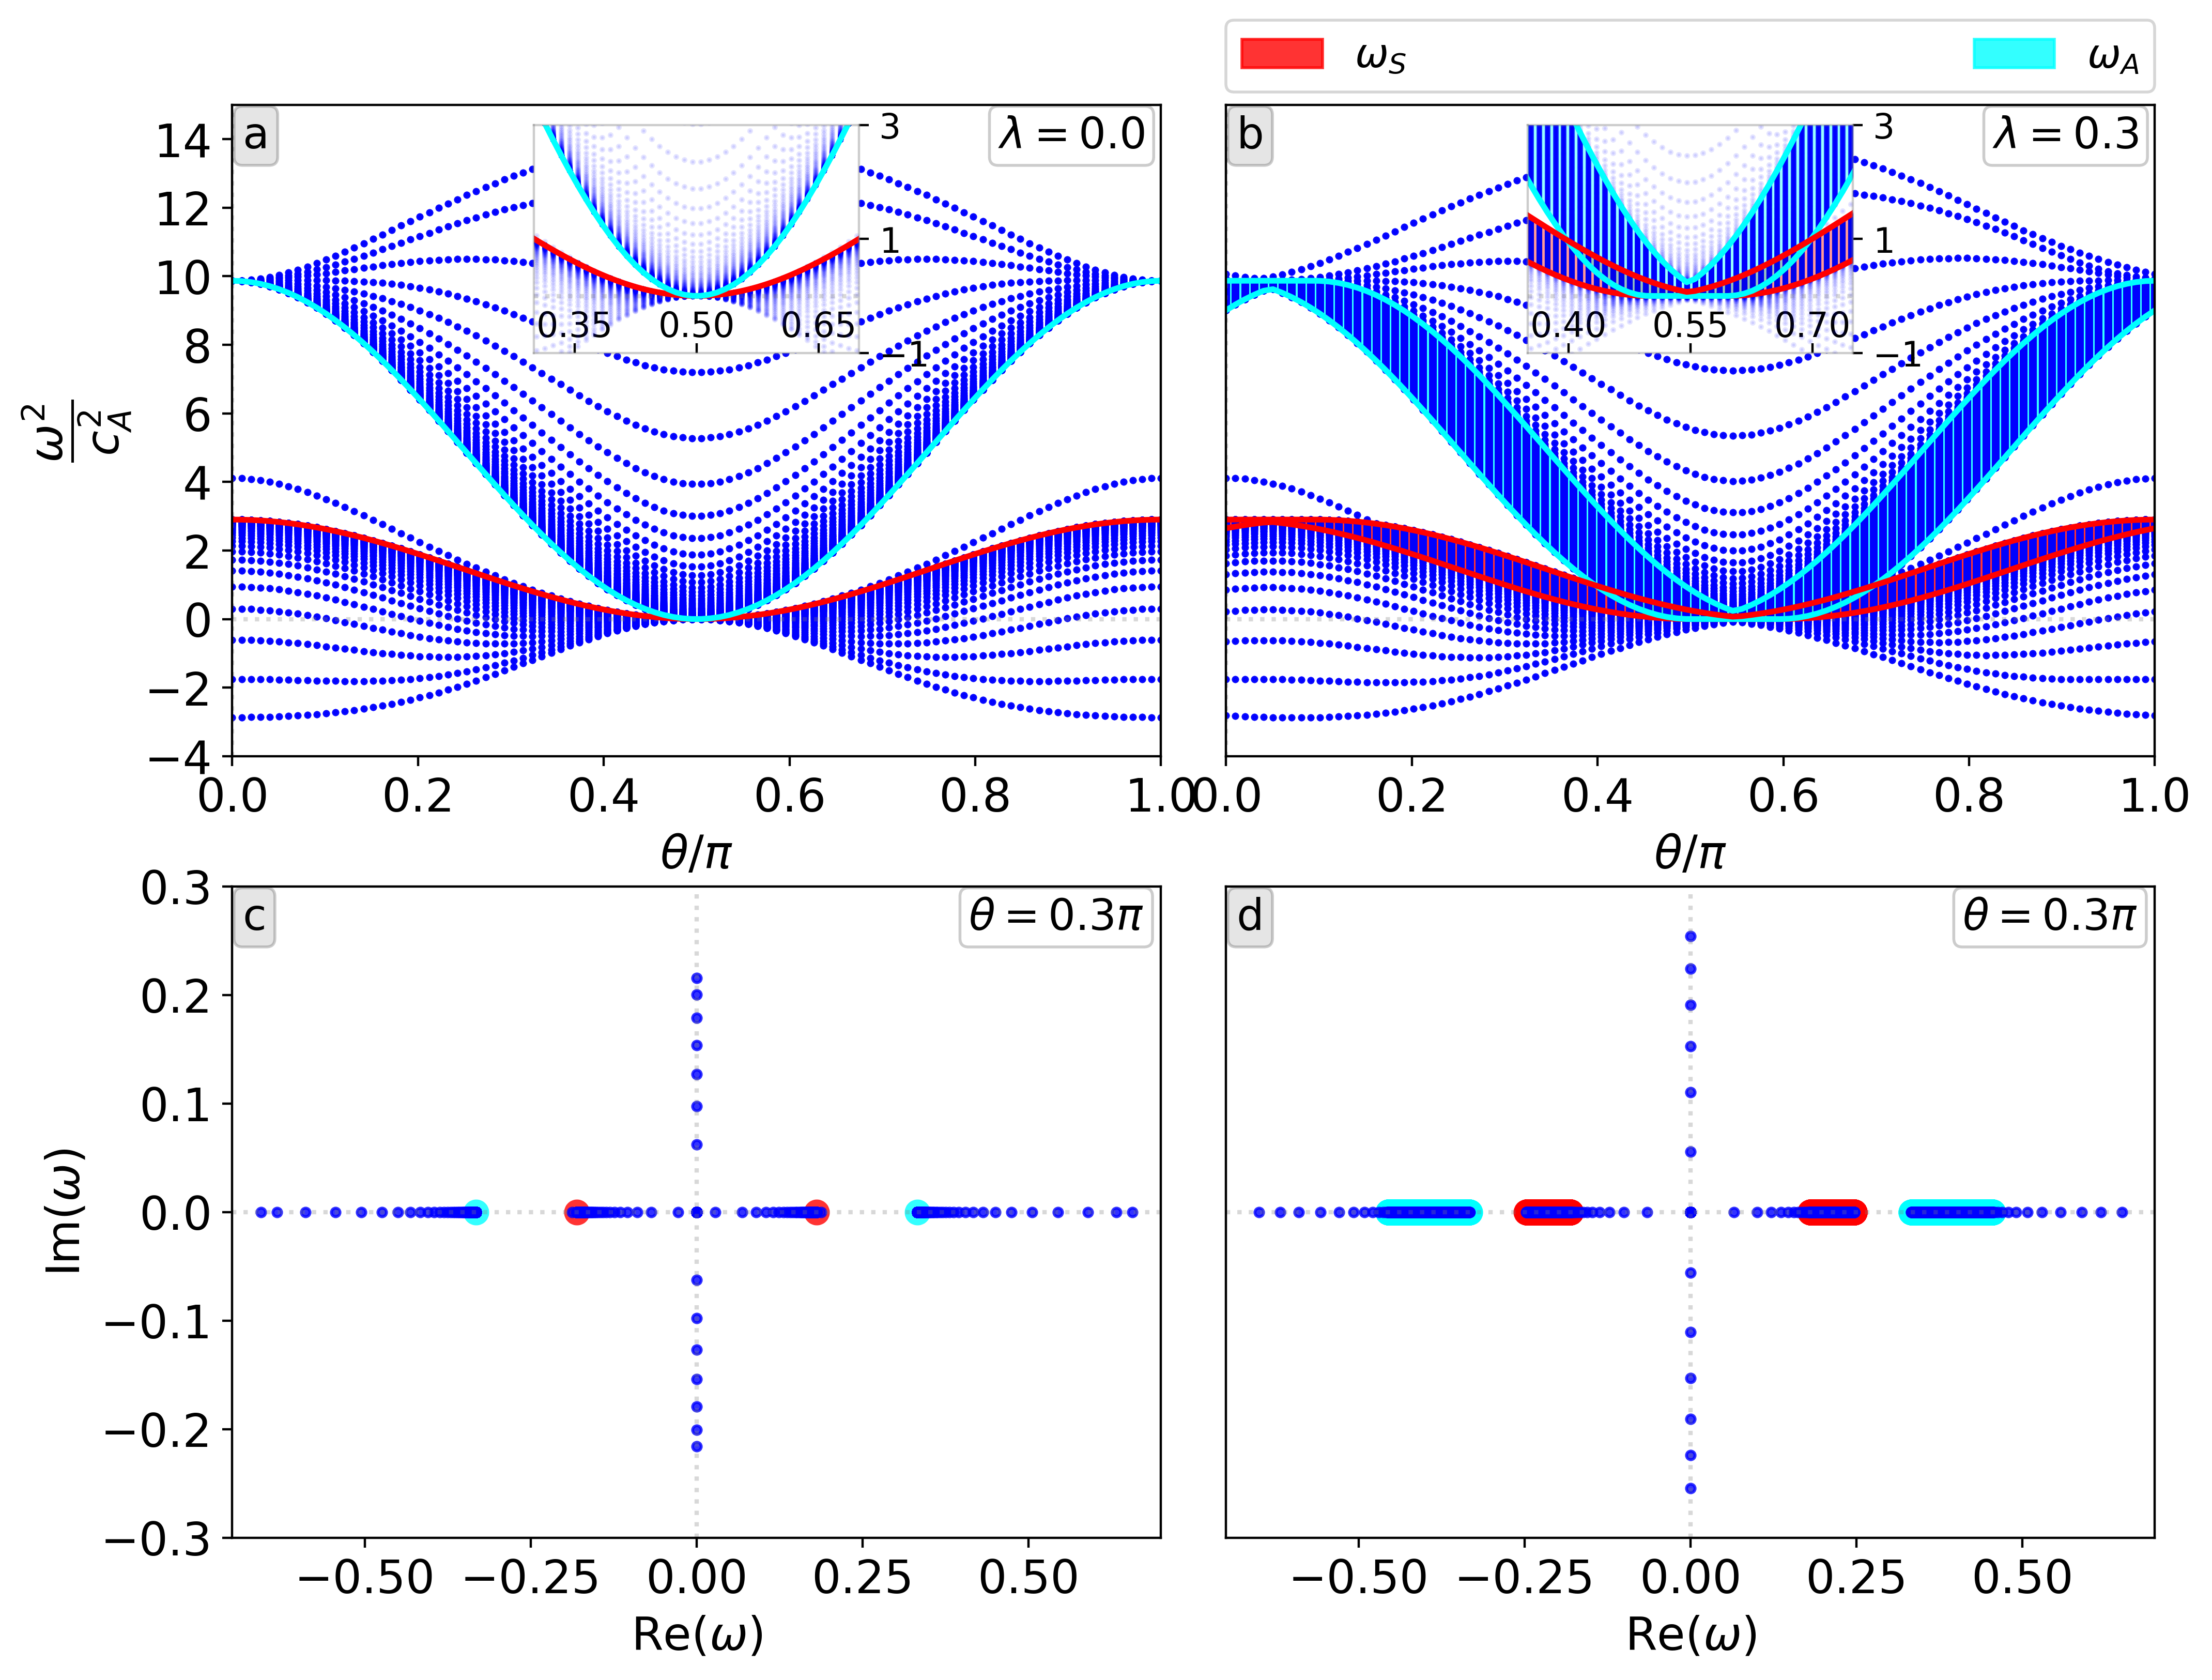
\includegraphics[width=\textwidth]{quasi_parker.png}
  \caption{
    Spectrum showing Parker and quasi-Parker modes without (\textbf{a}, \textbf{c}) and with (\textbf{b}, \textbf{d}) magnetic shear. The slow and Alfv\'en continua are shown in red and cyan, respectively, where the insets zoom into the region of quasi-interchange modes. The bottom row of panels show the eigenfrequency view for the single case $\theta = 0.3\pi$. The continua are again annotated in the panels, visualising the collapsed single point values (Panel \textbf{c}) as well as the genuine continuum ranges (Panel \textbf{d}).
  }
  \label{fig: quasi_parker}
\end{figure}

As explained in \citet{book_MHD}, we see from this eigenmode computation that the Parker instability, which is there for $\bk_0$ parallel to $\bb_0$, becomes a quasi-Parker instability away from perfect alignment and connects smoothly to well-known quasi-interchange instabilities that occur here (marginally) away from perpendicular orientation. Quantifying how the equilibrium parameters influence the growth rates of these unstable branches can only be done numerically, for example with {\legolas}.

\section{Adiabatic, cylindrical cases}
Next we move on to cylindrical configurations, which provide tests for the scale factor $\eps$ in the equations. Analytical results from the literature are again well reproduced. Furthermore, we look at different spectra previously obtained by the LEDA code, discussed in various papers, and compare those with the new spectra from {\legolas}.

\subsection{Magnetic flux tubes}
The first case that we describe in this subsection is a magnetic flux tube embedded in a uniform magnetic environment, discussed in \citet{book_roberts}. The equilibrium configuration is simple, in the sense that we have a uniform magnetic field aligned with the $z$-axis both inside and outside of the flux tube, with a similar structure for the other equilibrium parameters:
\begin{equation}
  B_0(r), \rho_0(r), p_0(r), T_0(r) =
  \begin{cases}
    B_0, \rho_0, p_0, T_0, \qquad &r < a \\
    B_\text{e}, \rho_\text{e}, p_\text{e}, T_\text{e}, \qquad &r > a
  \end{cases}
\end{equation}
where the subscripts ``0'' and ``e'' refer to values inside the tube and for the environment, respectively. The outer radius of the tube is denoted by $a$ and hence represents a discontinuous interface between the tube itself and the environment. Because total pressure balance should be preserved across the boundary, which is something that follows from Equation \eqref{eq: force_equilibrium}, this yields a relation between pressures and magnetic field components inside and outside of the tube, which in turn implies a connection between the plasma densities, sound speeds, and Alfv\'en speeds across the boundary:
\begin{equation} \label{eq: flux_tube_pbalance}
  p_0 + \frac{1}{2}B_0^2 = p_\text{e} + \frac{1}{2}B_\text{e}^2, \qquad\qquad
  \frac{\rho_e}{\rho_0} = \frac{\soundspeed^2 + \dfrac{1}{2}\gamma \alfvenspeed^2}{
    c_\text{se}^2 + \dfrac{1}{2}\gamma c_\text{Ae}^2},
\end{equation}
where $\soundspeed^2 = \gamma p_0 / \rho_0$ and $\alfvenspeed^2 = B_0^2 / \rho_0$ denote the sound speed and Alfv\'en speed, respectively, in which the values outside of the flux tube are used if there is a subscript e present.

It should be noted that this extremely simple equilibrium configuration is the standard case used in many solar coronal loop seismology efforts. This configuration simply has two uniform media (one inside the tube and one in its exterior), so it has no continuous spectra (they reduce to point values), but the interface makes it possible to again have surface modes that would be affected by true radial variation. Also note that these flux tubes have only stable waves, but we can distinguish between body and surface waves, depending on the variation of the eigenfunctions within the flux tube. In the exterior of the flux tube all eigenfunctions are exponentially varying.

We should also clarify here that the original dispersion relation as given in \citet{book_roberts} assumes a flux tube embedded in an environment extending towards infinity, while {\legolas} on the other hand assumes a fixed wall boundary at the outer edge of the domain. Hence, we assume here that the domain is situated in $r \in [0, 10]$ with the inner flux tube wall at $r = 1$ in order to minimise the outer wall influence. However, this introduces an additional computational challenge, in the sense that we are (mainly) interested in the behaviour of the inner modes, because we know that the outer modes all have exponentially varying eigenfunctions which decay to infinity (or toward our far-away outer wall). Hence, in order to resolve those inner waves huge resolutions are needed due to the $1:10$ ratio. In order to circumvent this issue we used a simple prescription for mesh refinement, that is, a 60--30--10 division of the initial nodes. This means that $60\%$ of the grid points are used for the inner tube region $r \in [0, 0.95]$, $30\%$ of the grid points are located near the transition region $r \in [0.95, 1.05]$, and the remaining $10\%$ are used for the environment $r \in [1.05, 10]$.

\paragraph{(a) Photospheric flux tube.}
First, we look at a flux tube under photospheric conditions, that is, an equilibrium for which $c_\text{Ae} < \soundspeed < c_\text{se} < \alfvenspeed$. More specifically, we take $c_\text{Ae} = \soundspeed/2$, $c_\text{se} = 3\soundspeed / 2$, and $\alfvenspeed = 2\soundspeed$ following \citet[Figure 6.5]{book_roberts}. The relations between the inner and outer regions of the flux tube follow straightforwardly from Equation \eqref{eq: flux_tube_pbalance}, and hence we only have two degrees of freedom, namely $\rho_0$ and $p_0$, which are both taken to unity, with $\gamma = 5/3$. This results in $\rho_0 \approx 0.567~\rho_\text{e}$, $\tubespeed \approx 0.89~\soundspeed$,
$\kinkspeed \approx 0.63~\alfvenspeed \approx 1.27~\soundspeed$. Here we also introduced the tube and kink speeds, given by
\begin{equation}
  \tubespeed^2 = \frac{\soundspeed^2 \alfvenspeed^2}{\soundspeed^2 + \alfvenspeed^2}, \qquad\qquad
  \kinkspeed^2 = \frac{\rho_0 \alfvenspeed^2 + \rho_\text{e}c_\text{Ae}^2}{\rho_0 + \rho_\text{e}},
\end{equation}
using the same notation as in Equation \eqref{eq: flux_tube_pbalance}. As described before, we take $r \in [0, 10]$ and place the flux tube boundary at $a = 1$. Next we perform 40 runs at 300 gridpoints each for four azimuthal wavenumbers $m = 0$ to $m = 3$. For the wavenumber $k_3 = k_z$, we take 40 values in such a way that the dimensionless wavenumber $k_z a$ has values in $[0, 6.2]$. The spectrum showing the dispersion relation, where the dimensionless phase speed $\omega / k_z \soundspeed$ is plotted as a function of $k_z a$, is depicted in Figure \ref{fig: fluxtube_coronal}.

\begin{figure}[t]
  \centering
  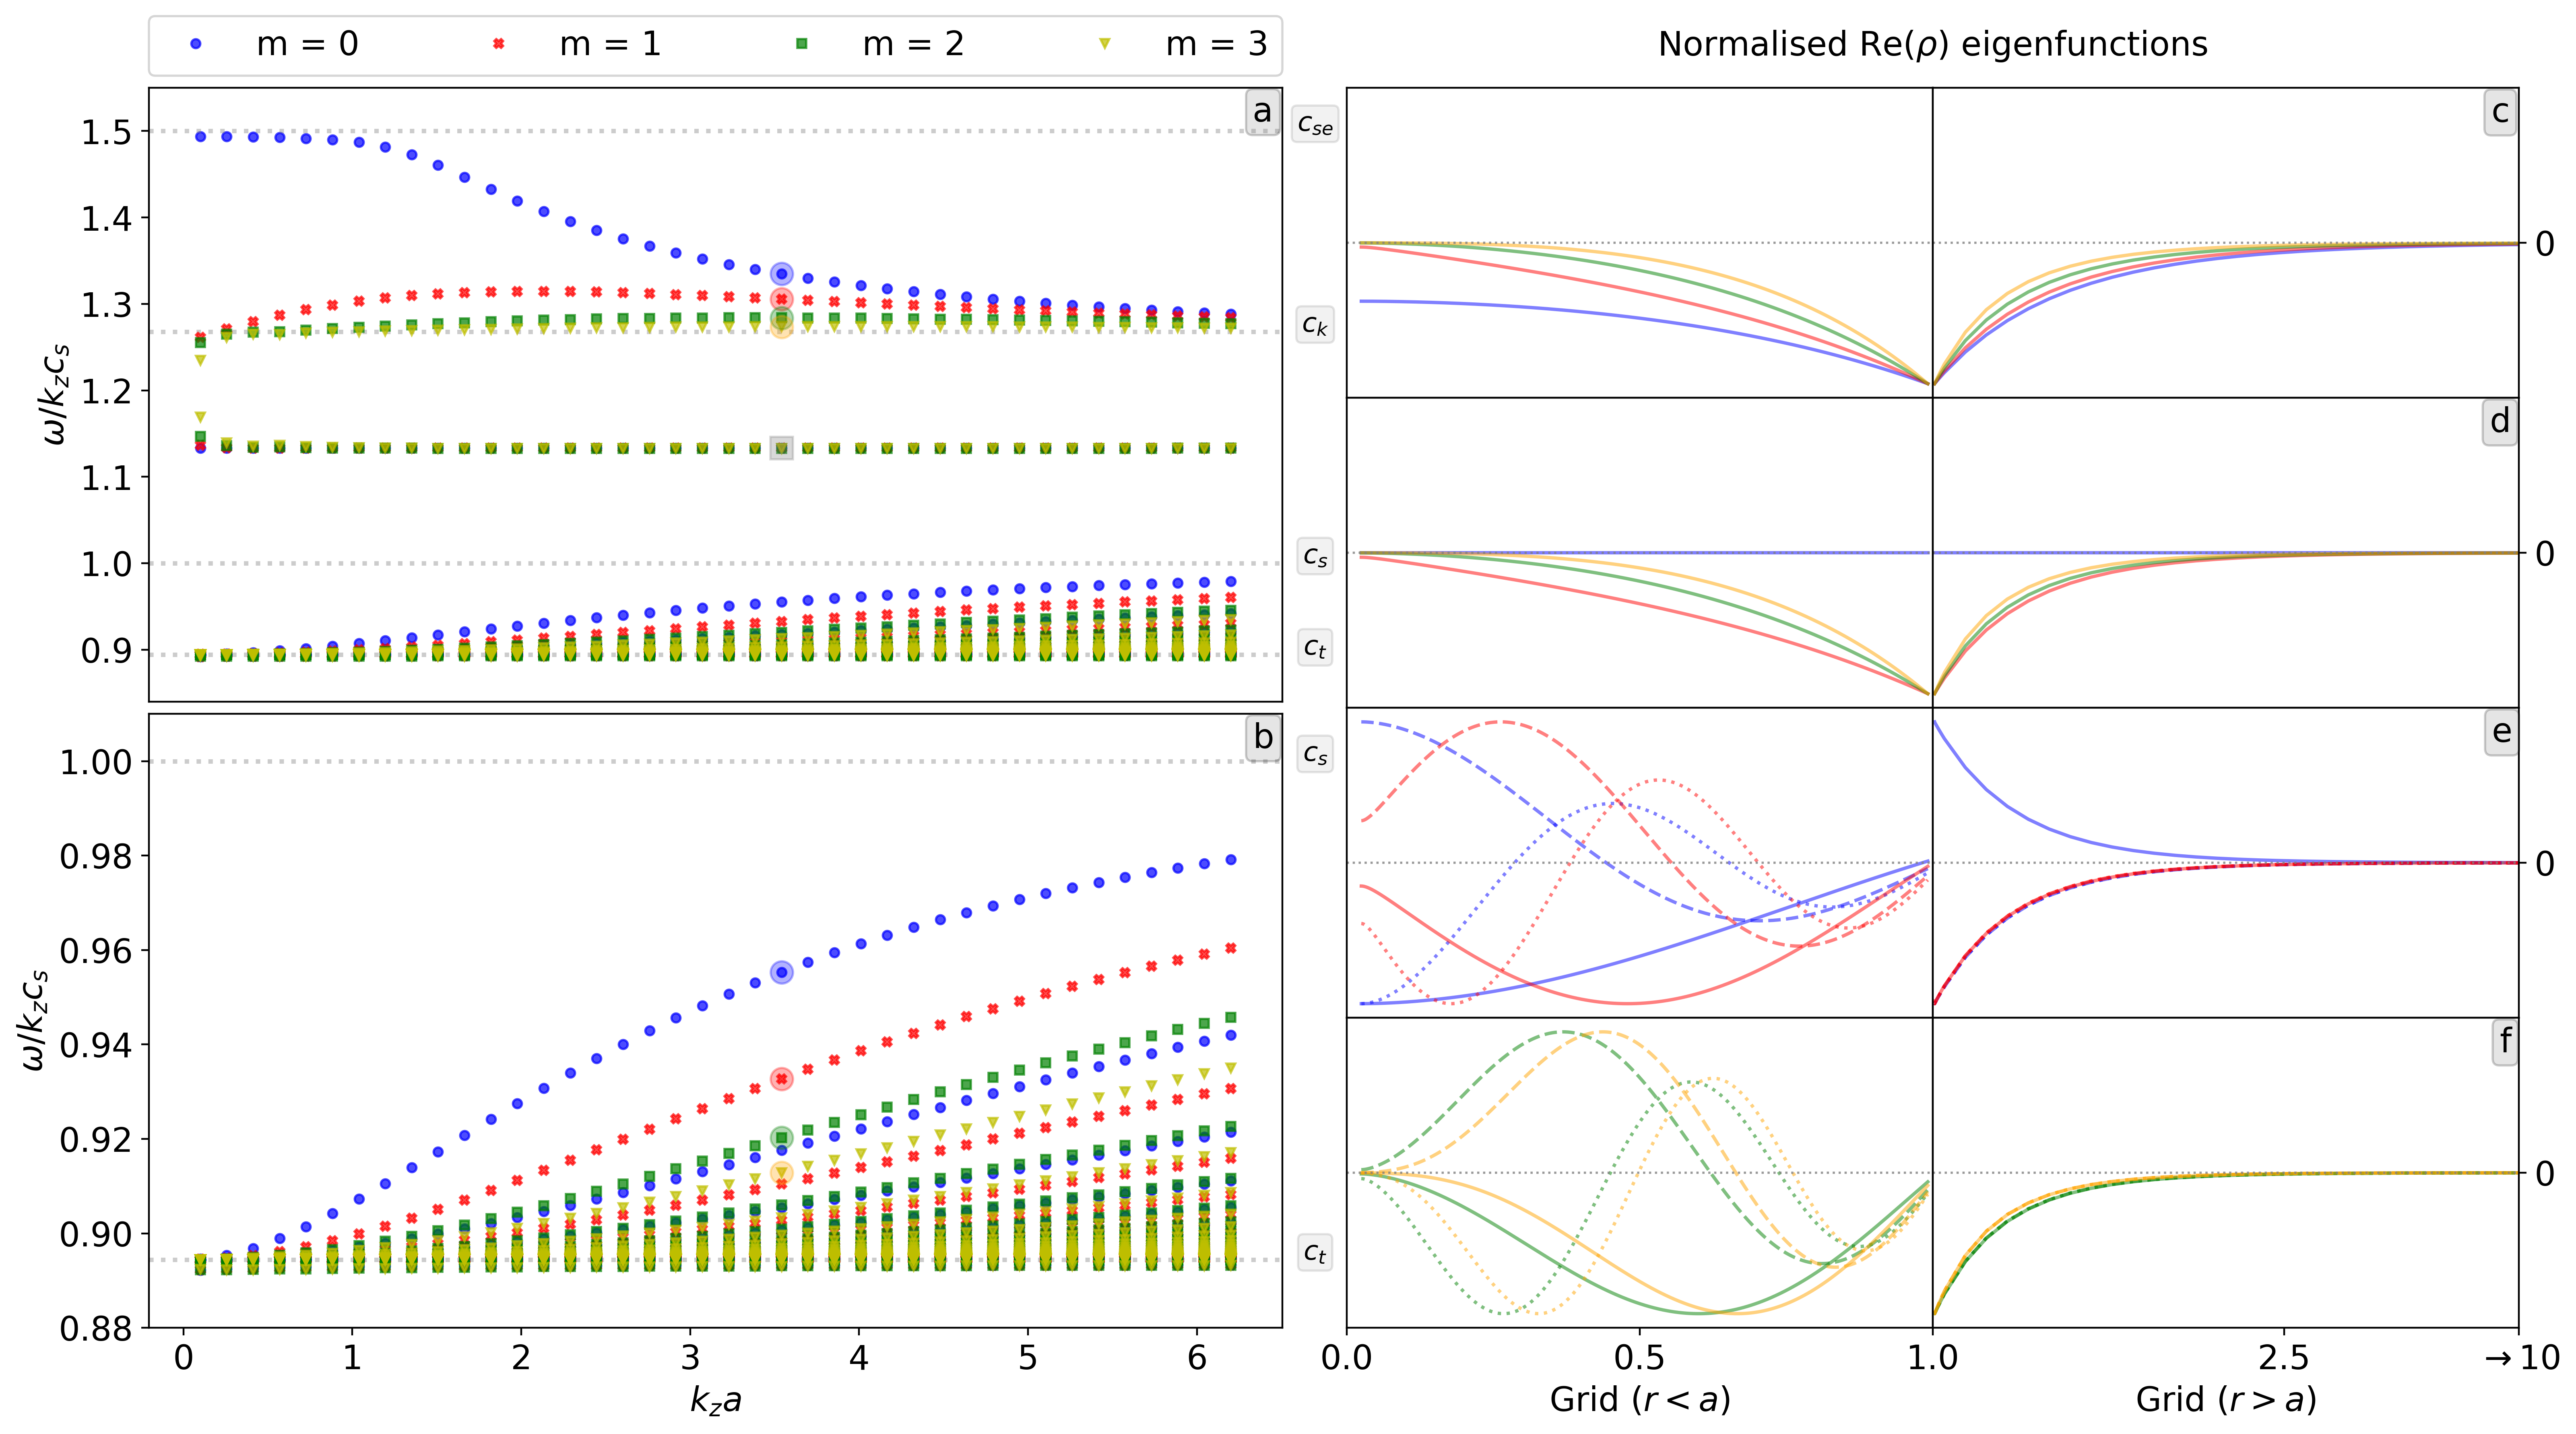
\includegraphics[width=\textwidth]{fluxtube_photospheric.png}
  \caption{
    Panel \textbf{a}: spectrum showing the dispersion relation for a flux tube under photospheric conditions. The dimensionless phase speed $\omega / k_z \soundspeed$ is displayed as a function of the dimensionless wavenumber $k_z a$ for four values of the azimuthal wavenumber $m = 0$ (blue dots), $m = 1$ (red crosses), $m = 2$ (green squares), and $m = 3$ (yellow triangles). Both sound speeds, the kink speed, and the tube speed are denoted using dashed grey horizontal lines, all normalised to $\soundspeed$. Panel \textbf{b}: zoom-in of Panel \textbf{a} between the tube speed $\tubespeed$ and internal sound speed $\soundspeed$. Panels \textbf{c} and \textbf{d}: eigenfunctions of the modes associated with circles (\textbf{c}) and squares (\textbf{d}) on the top-left Panel \textbf{a}. Panel \textbf{e}: first three eigenfunctions of the $m = 0$ and $m = 1$ body wave sequence on Panel \textbf{b}. Panel \textbf{f}: first three eigenfunctions of the $m = 2$ and $m = 3$ body wave sequence. For both panels \textbf{e} and \textbf{f}, the $n = 1$, $n = 2$, and $n = 3$ modes are shown in solid, dashed and dotted lines, respectively; only the first mode is annotated on the bottom-left Panel. Every eigenfunction in panels \textbf{c}--\textbf{f} is normalised to its maximum absolute value in that particular grid interval.
  }
  \label{fig: fluxtube_photospheric}
\end{figure}

All speeds indicated in the figure are normalised to the internal sound speed $\soundspeed$. Panel a clearly shows the fast surface waves, including the sausage $(m = 0)$, kink $(m = 1)$, and first two fluting modes ($m = 2$ and $m = 3$). The eigenfunctions in Panel c correspond to the modes annotated with a transparent circle in Panel a, with colours indicating the mode number $m$. The left and right sides of Panels c--f show the eigenfunctions for the inner and outer regions of the flux tube, respectively. All eigenfunctions are normalised to their maximum value, and all eigenvalues having a normalised phase speed larger than 1.5 are not shown. It should be noted that the first three runs, that is, the first three dots according to the $k_z a$ axis, were performed using 1001 gridpoints. The reason for this is that when we divide the eigenvalues $\omega$ by $k_z$, small errors are increased selectively for small $k_z$, explaining why those modes seem slightly scattered and hence why he have to employ such high resolutions in order to minimise said error.

Panel b of Figure \ref{fig: fluxtube_photospheric} zooms in between the tube speed ($\tubespeed$) and internal sound speed ($\soundspeed$), showing a clear representation of the various body waves that accumulate to the tube speed at long wavelengths. Panel e shows the first three modes of the $m = 0$ and $m = 1$ sequences in solid, dashed, and dotted lines, respectively; that is, the first mode in the sequence (solid line) corresponds to the mode annotated in Panel b. The next two modes in that sequence are the next two blue dots moving vertically downwards (same $k_z a$ value), these are not annotated to avoid cluttering the figure. Analogously, Panel f shows the first three modes of the $m = 2$ and $m = 3$ sequences, with everything colour-coded according to the legend. As indicated before, all eigenfunctions in the outer region are exponentially varying. Panels a and b in Figure \ref{fig: fluxtube_photospheric} reproduce the analytical results in \citet[Figure 6.5]{book_roberts}.

One mode has not yet been discussed, and that is the horizontal line of modes between the internal sound speed and kink speed. The eigenfunctions are shown in Panel d and correspond to the annotated squares in the top-left Panel a. These modes are not present in the original work, and it is not a priori clear how to interpret them. These modes are degenerate, meaning that their position does not change when the mode number $m$ or wavenumber $k_z$ changes. The position of the outer wall also does not seem to have any influence on their value, and their eigenfunctions seem to indicate that these are surface waves. However, it is also quite possible that these modes are a numerical remnant of the discontinuous equilibrium profile, and are picked up by {\legolas} due to the sharp transition between the inner flux tube and the environment at $a = 1$.

\paragraph{(b) Coronal flux tube.} The second application of the magnetic flux tube is one under coronal conditions, that is, an equilibrium for which $c_\text{se} < \soundspeed < \alfvenspeed < c_\text{Ae}$. More specifically, we take
$c_\text{Ae} = 5\soundspeed$, $c_\text{se} = \soundspeed/2$, and $\alfvenspeed = 2\soundspeed$. Analogous to the previous case, the relations between the equilibrium values inside and outside of the flux tube follow from Equation \eqref{eq: flux_tube_pbalance}, where we again take $p_0$ and $\rho_0$ to be equal to one. This results in
$\rho_0 \approx 4.86~\rho_\text{e}$, $\tubespeed \approx 0.89~\soundspeed$,
$\kinkspeed \approx 1.38~\alfvenspeed \approx 0.55~c_\text{Ae}$; we use the same values as for the photospheric case for $k_z$ and the flux tube and outer wall boundaries.
\begin{figure}[t]
  \centering
  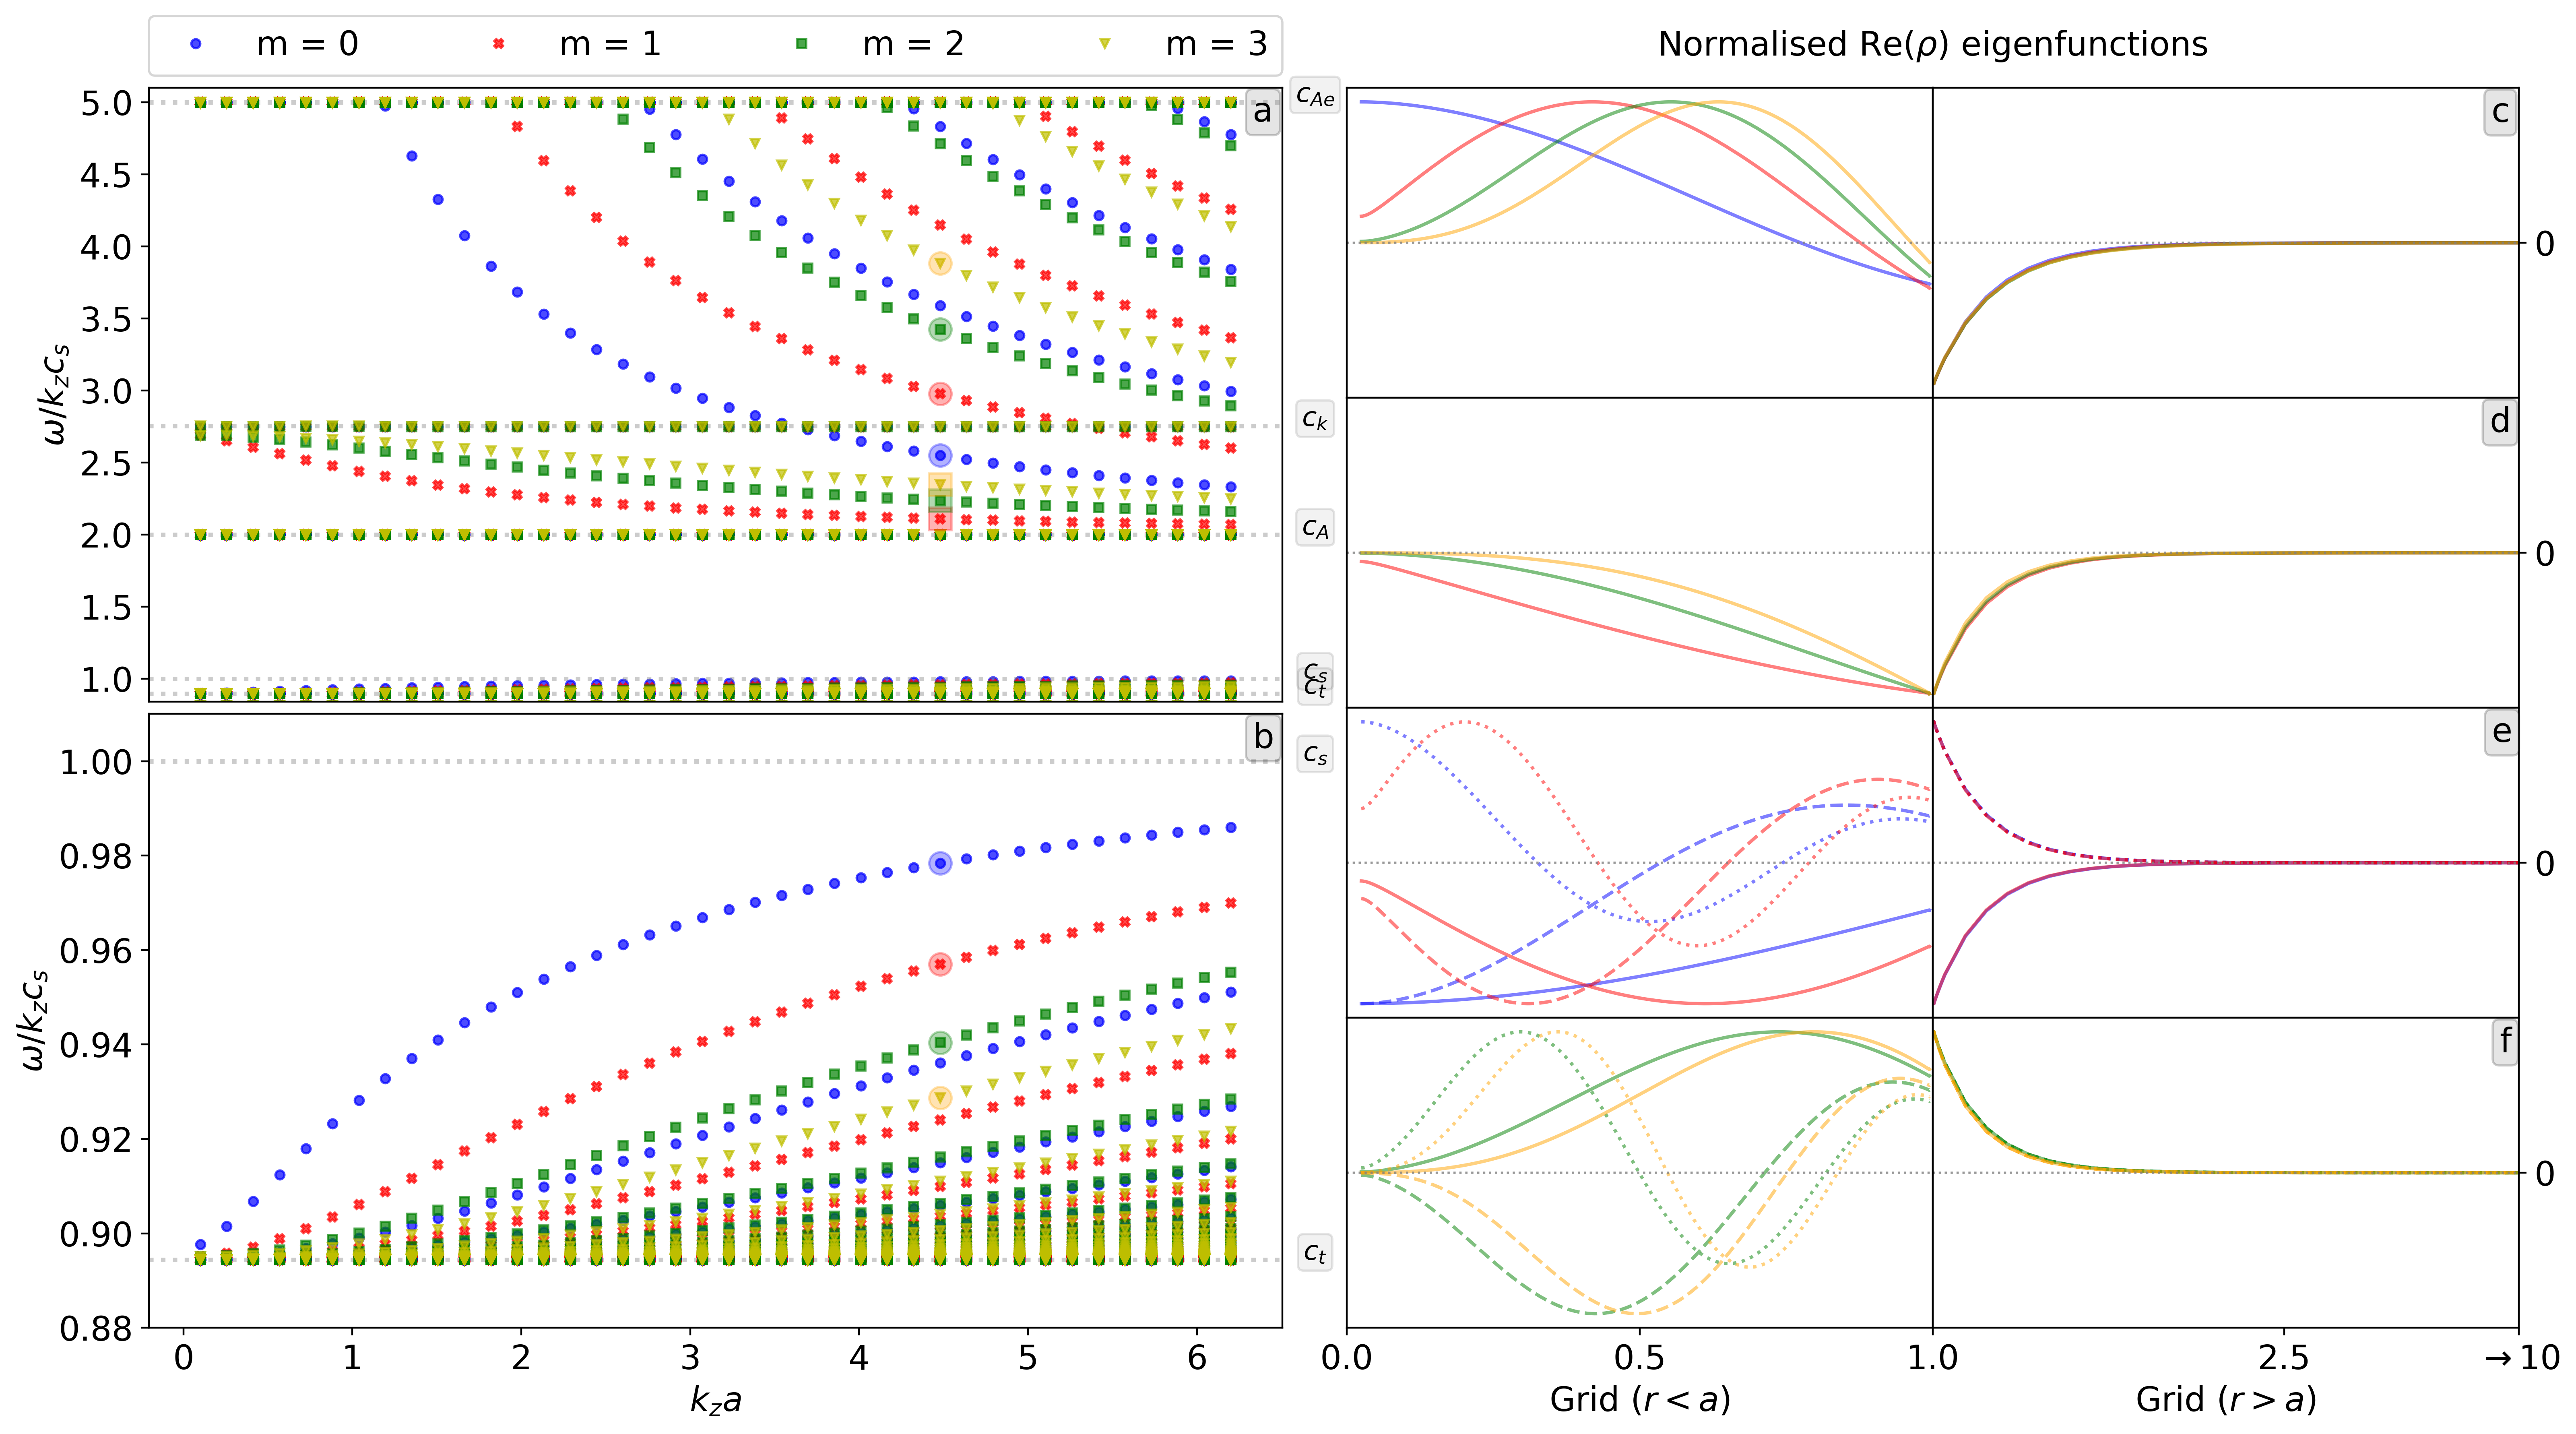
\includegraphics[width=\textwidth]{fluxtube_coronal.png}
  \caption{
    Panel \textbf{a}: spectrum showing the dispersion relation for a flux tube under coronal conditions. The dimensionless phase speed $\omega / k_z \soundspeed$ is displayed as a function of the dimensionless wavenumber $k_z a$ for four values of the azimuthal wavenumber $m = 0$ (blue dots), $m = 1$ (red crosses), and $m = 2$ (green squares), and $m = 3$ (yellow triangles). Both Alfv\'en speeds, together with the kink, tube, and sound speeds are denoted by grey horizontal lines and are all normalised to $\soundspeed$. Panel \textbf{b} zoom-in of Panel \textbf{a} between the tube speed $\tubespeed$ and internal sound speed $\soundspeed$, zooming in on the tube-speed-related body mode sequences. Panels \textbf{c} and \textbf{d}: eigenfunctions of the modes annotated with circles (\textbf{c}) and squares (\textbf{d}) on the top-left Panel \textbf{a}. Panel \textbf{e}: first three eigenfunctions of the $m = 0$ and $m = 1$ body wave sequence in the bottom-left Panel \textbf{b}. Panel \textbf{f}: first three eigenfunctions of the $m = 2$ and $m = 3$ body wave sequence. For both Panels \textbf{e} and \textbf{f} the $n = 1$, $n = 2$ and $n = 3$ modes are shown in solid, dashed and dotted lines, respectively, only the first mode is annotated on Panel \textbf{b}. Every eigenfunction in Panels \textbf{c}--\textbf{f} is normalised to its maximum absolute value in that particular grid interval.
  }
  \label{fig: fluxtube_coronal}
\end{figure}
Similar to case (a), we perform 40 runs at 300 gridpoints each for four values of $k_2 = m$ (where again the first three runs have 1001 gridpoints) and plot the spectrum showing the dispersion relation in Figure \ref{fig: fluxtube_coronal}. Again, all speeds indicated in the figure are normalised to the sound speed $\soundspeed$. The top-left Panel a focuses on the fast body waves, the bottom-left Panel b on the slow body waves. Panel c shows the eigenfunctions corresponding to the four body waves indicated with circles in Panel a. Panel d depicts the eigenfunctions of the modes annotated with squares between the internal Alfv\'en ($\alfvenspeed$) and kink ($\kinkspeed$) speeds, representing the kink $m = 1$ and first two fluting ($m = 2$ and $m = 3$) modes.

Similar to Figure \ref{fig: fluxtube_photospheric}, Panels e and f represent the first three body modes in the $m = 0$ and $m = 1$ sequences (Panel e), of which the first mode is indicated in Panel b. Panel f shows the first three modes of the $m = 2$ and $m = 3$ sequences, with the first, second, and third modes indicated with a solid, dashed and dotted line, respectively. The colours of Panels c--f are consistent with the legend. Figure \ref{fig: fluxtube_coronal} reproduces the analytical results in \citet[Figure 6.7]{book_roberts}, which are based on the analytic dispersion relation containing Bessel functions.

\subsection{Tokamak current profile}
Next we discuss an example initially given in \citet{kerner1985}, which shows the ideal MHD spectrum in the presence of an unstable $m = -2$ interchange mode in a cylindrical geometry. We start from a so-called tokamak current profile, in which an axial current density of the form $\boldsymbol{j}_0 = \left(0, 0, j_0(1 - r^2)^\nu\right)$ is assumed, with $j_0$ a given constant. This yields a twisted magnetic field profile in which the longitudinal component $B_{0z}$ is uniform and equals one, while the poloidal component $B_{0\theta}$ is given by
\begin{equation} \label{eq: tokamak_btheta}
  B_{0\theta} = \frac{j_0}{2r\left(\nu + 1\right)}\left[1 - \left(1 - r^2\right)^{\nu + 1}\right],
\end{equation}
for a given value of $\nu$. For the equilibrium considered here, we take $\nu = 0$, making the current profile constant over the flux tube. This means that $B_{0\theta}$ has a linear profile in $r$ such that the magnetic field lines have a constant pitch and the current is distributed equally in the plasma. An expression for the pressure (and hence temperature) can be found by integrating the force-balance Equation \eqref{eq: force_equilibrium} and assuming that, for example, the pressure vanishes at the outer boundary, resulting in a parabolic pressure profile. Hence, for a cylindrical geometry in which $r \in [0, 1]$, this yields the following equilibrium configuration:
\begin{equation}
  \begin{gathered}
    \rho_0 = 1,
    \qquad
    p_0 = \frac{1}{4}j_0^2\left(1 - r^2\right),
    \qquad
    B_{02} = \frac{1}{2}j_0 r,
    \qquad
    B_{03} = 1,
  \end{gathered}
\end{equation}
where we assumed a uniform density. We introduce an additional parameter $q$, called the \emph{safety factor}, given by
\begin{equation}
  q(r) = \frac{rk_z B_{0z}}{B_{0\theta}} = \frac{2k_z}{j_0}.
\end{equation}

We performed 39 runs, varying the $q$ factor between 1.9 and 2.1 in order to probe the regime containing the unstable $m = -2$ interchange mode, which is associated with the vanishing of the $\bk \cdot \bb_0$ product. This implicitly constrains the value for $j_0$, and we assigned $k_2 = m = -2$ and $k_3 = k = 0.2$ for all runs. It should be noted that this particular equilibrium configuration requires a relatively high resolution near $q = 2$ to correctly resolve the unstable modes; here we used 501 gridpoints for all runs. The complete spectrum is shown in Figure \ref{fig: tokamak_current}, where the squared eigenvalues are plotted as a function of the safety factor. The three main branches, that is, fast, Alfv\'en and slow, are denoted on the right side of the figure, as well as the region where the modes become unstable $(\omega^2 < 0)$. We see that in the region near the $m = -2$ interchange instabilities, the slow and Alfv\'en modes collapse to zero, which is due to the vanishing of the combination $\Fplus$ (see Equation \eqref{eq: F_G_operators} in Chapter \ref{ch: legolas}) in the ideal MHD equations \citep{book_MHD}. The slow and Alfv\'en continua are annotated in the figure in red and cyan, respectively. The Alfv\'en continuum is collapsed to a single point for this equilibrium configuration, while the slow continuum covers a range in frequency. Note in particular how the full spectrum ranges over many orders of magnitude in the $\omega^2$ view shown here: an intrinsic property (and challenge!) posed by MHD spectral theory.

\begin{figure}[t]
  \centering
  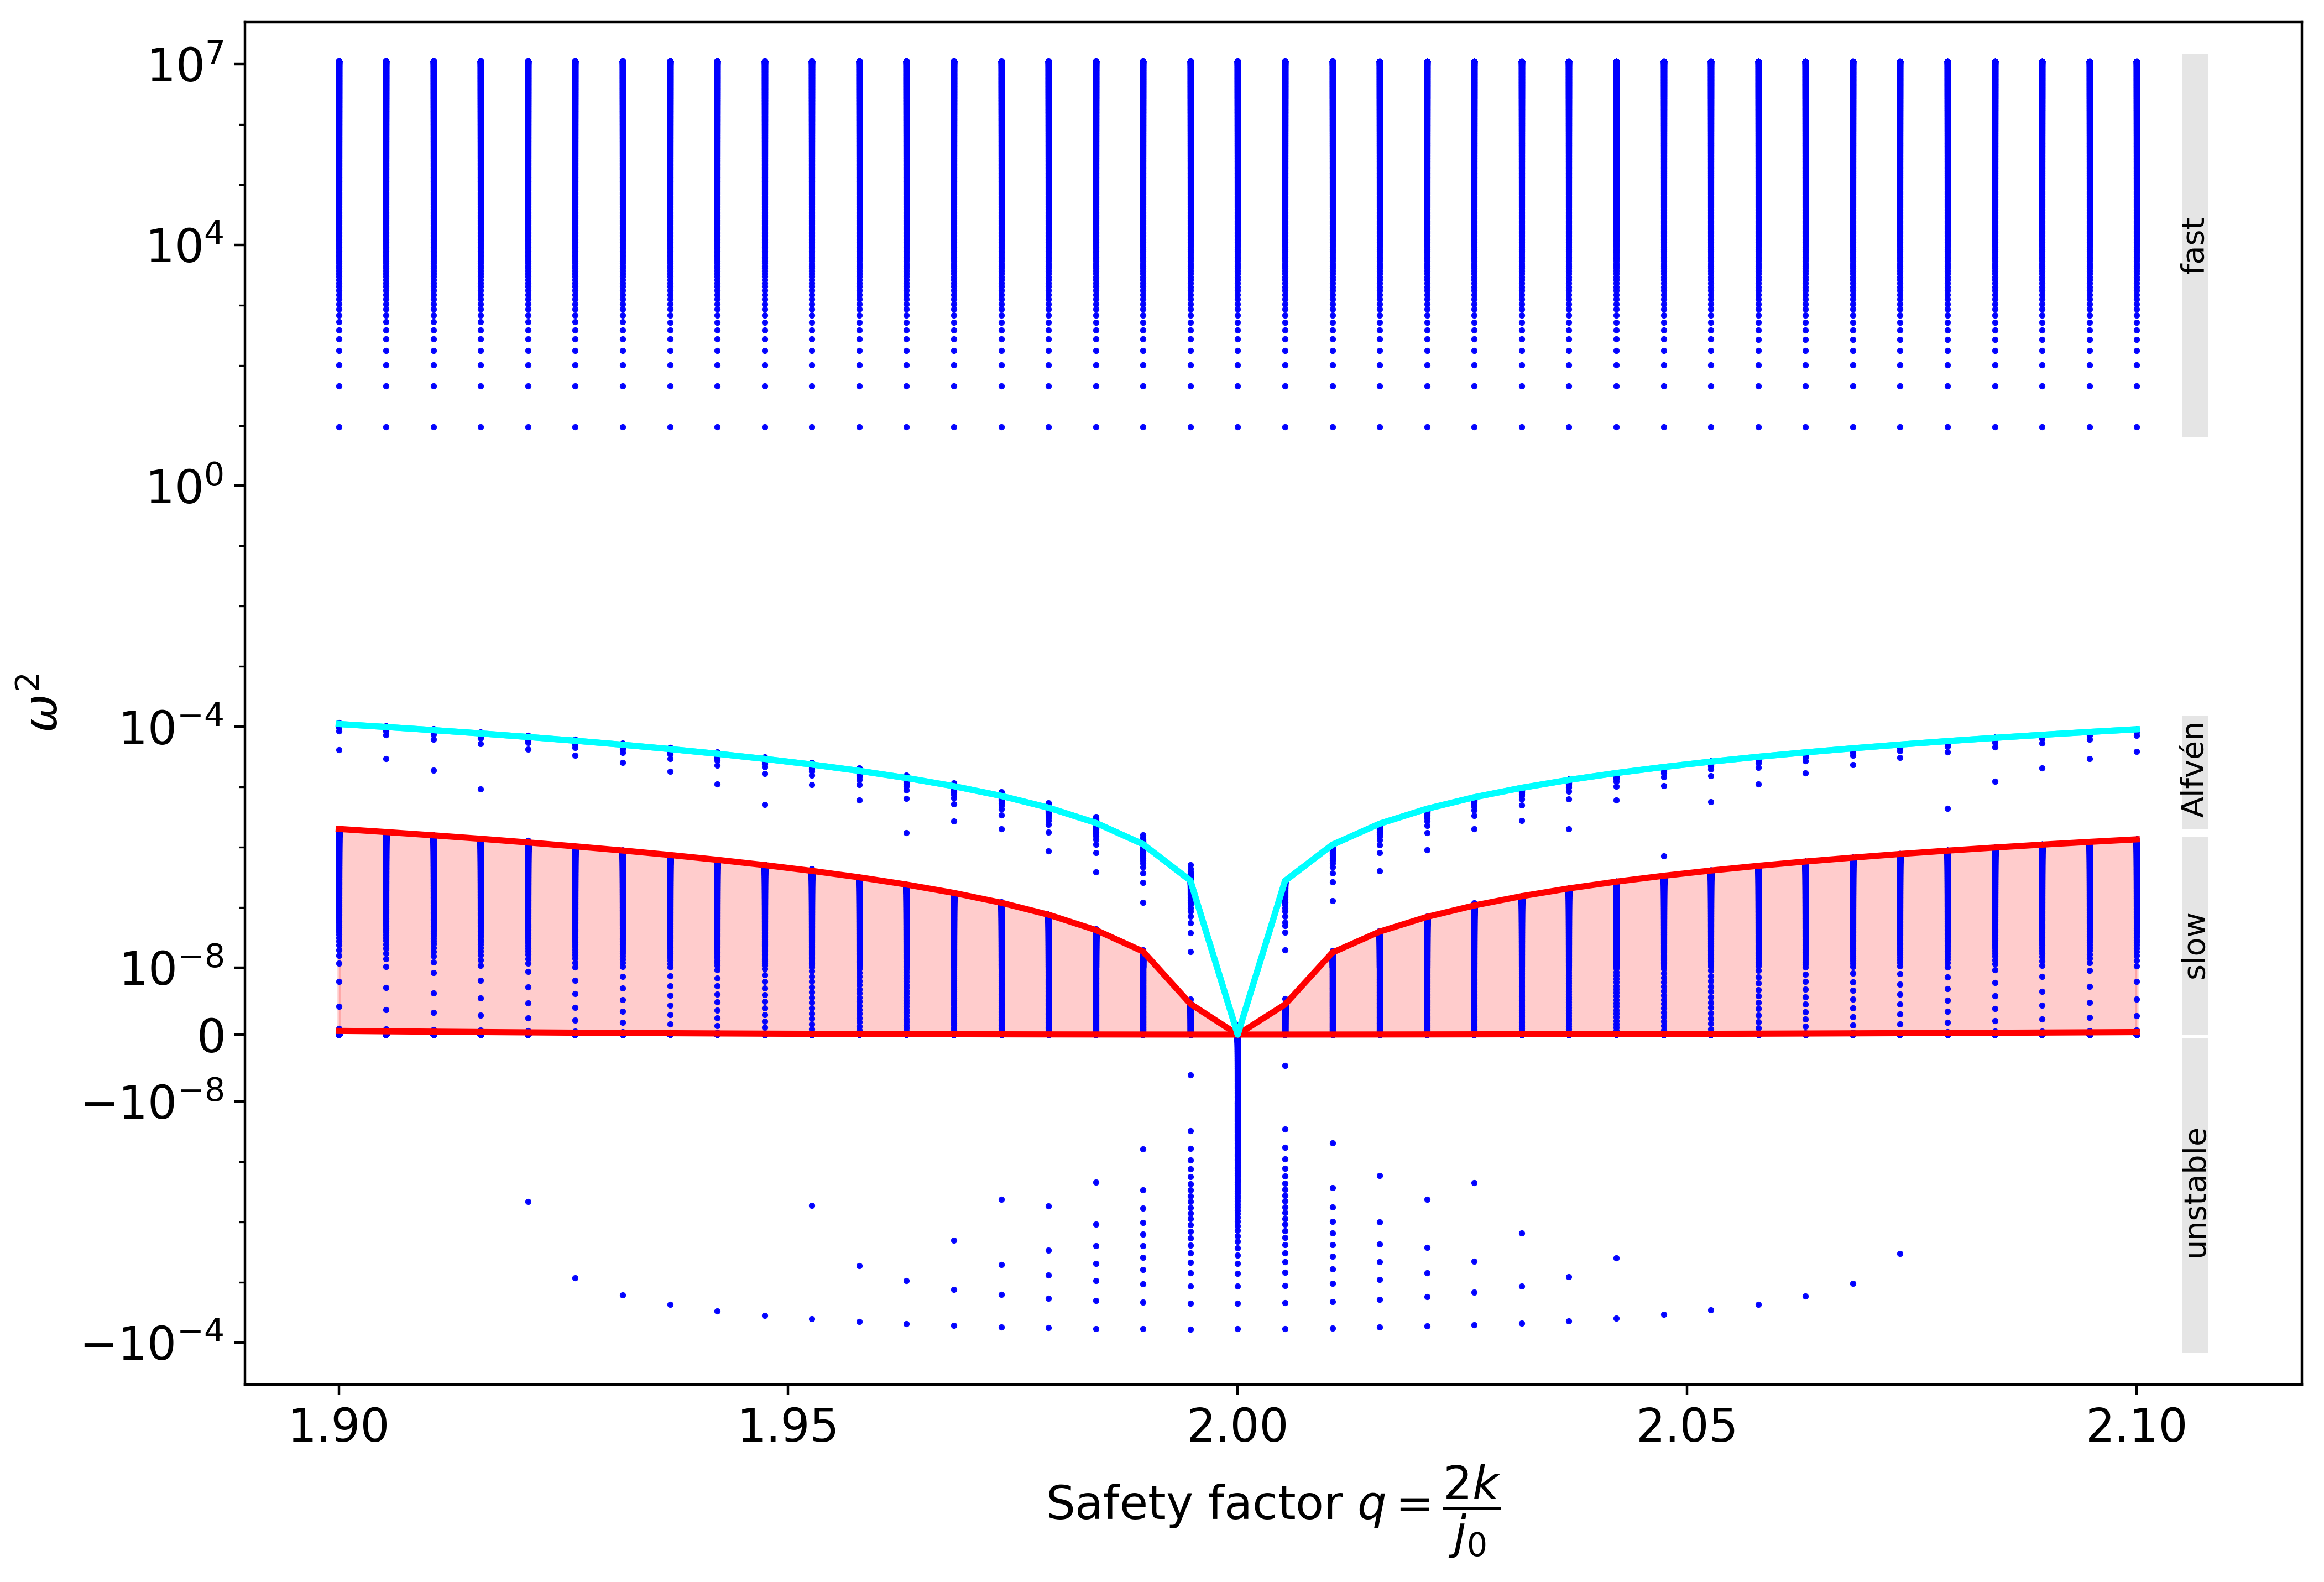
\includegraphics[width=\textwidth]{kerner_tokamak.png}
  \caption{
    Complete MHD spectrum for a tokamak current profile in the presence of the $m = -2$ interchange mode. The squared eigenvalues are plotted against the safety factor $q$, instabilities correspond to $\omega^2 < 0$. The various branches are indicated on the right side of the figure.
  }
  \label{fig: tokamak_current}
\end{figure}

\subsection{KH and CD instabilities} \label{ss: kh_cd_instabilities}
As a first test for the inclusion of flow into the equations, we look at the interaction between the KHIs and current-driven (CD) instabilities in a magnetised astrophysical jet, following \citet{baty2002}. This model uses a cylindrical jet with a supersonic background flow aligned with the axis and sheared in the radial direction. The equilibrium configuration is taken such that Kelvin-Helmholtz surface modes can develop and is generally given by
\begin{equation} \label{eq: kh_cd_equilibrium}
  \begin{gathered}
    \rho_0 = 1,
    \qquad
    v_{02} = 0,
    \qquad
    v_{03} = \frac{1}{2}\mathcal{V}\tanh\left(\frac{r_j - r}{a}\right),
    \qquad
    B_{03} = B_{0z}, \\
    B_{02} = B_{0\theta} \frac{r r_c}{r_c^2 + r^2},
    \qquad
    T_0 = \frac{p_0}{\rho_0} - \frac{B_{0\theta}^2}{2\rho_0}\left(1 - \frac{r_c^4}{\left(r_c^2 + r^2\right)^2}\right).
  \end{gathered}
\end{equation}
Here, $r_j$ denotes the jet radius and $r_c$ quantifies the radial variation, taken to be $r_j = 1$ and $r_c = 0.5$, with $r \in [0, 2]$. The parameter $\mathcal{V}$ represents the amplitude of the velocity, given by $\mathcal{V} = 1.63$, while the chosen velocity profile ensures that the shear layer is situated at the jet radius with a radial width given by $a = 0.1r_j$. Both the density $\rho_0$ and the pressure on-axis $p_0$ are chosen to be equal to unity. The parameters $B_{0\theta}$ and $B_{0z}$ control the amplitude and twist of the magnetic field, as explained in \citet{baty2002}. The original work discusses three different magnetic field configurations, we choose the profile with
\begin{equation}
  B_{0\theta} = 0.4\left(\frac{r_c^2 + r_j^2}{r_j r_c}\right),
  \qquad
  B_{0z} = 0.25,
\end{equation}
such that $B_{02} = 0.4$ at the jet radius. Furthermore, the azimuthal and longitudinal wavenumbers are taken to be $k_2 = m = -1$ and $k_3 = k = \pi$.

The entire spectrum is calculated using 501 gridpoints and shown in Figure \ref{fig: kh_cd}. Panel a depicts the full slow and Alfv\'en spectra with the KH and first three CD unstable modes ($\omega_\text{I} > 0$) denoted on the figure itself. The real and imaginary parts of the $\rho$, $r v_r$, and $v_z$ eigenfunctions for each of these modes are shown on the subsequent panels. Those for the KH mode (Panels c--d) are localised around the jet radius $r = 1$, which is also the point where the Alfv\'enic Mach number drops to zero (Panel b). The quantity $V_0$ in the Figure legend represents the velocity magnitude, here given by $V_0 = \sqrt{v_{02}^2 + v_{03}^2}$. Panels e through j depict the eigenfunctions of the first three CD modes, with the first, second, and third shown in the first, second, and third rows of the bottom panels, respectively. The left column shows the real part, the right column the imaginary part of the eigenfunction. The CD modes have an increasing number of nodes on $r \in [0, 1]$, which is most clearly visible by looking at the
$r v_r$ eigenfunction (green): no nodes for the first CD mode (Panels e--f), one node for the second CD mode (Panels g--h), and two nodes for the third CD mode (Panels i--j).

\begin{figure}[t]
  \centering
  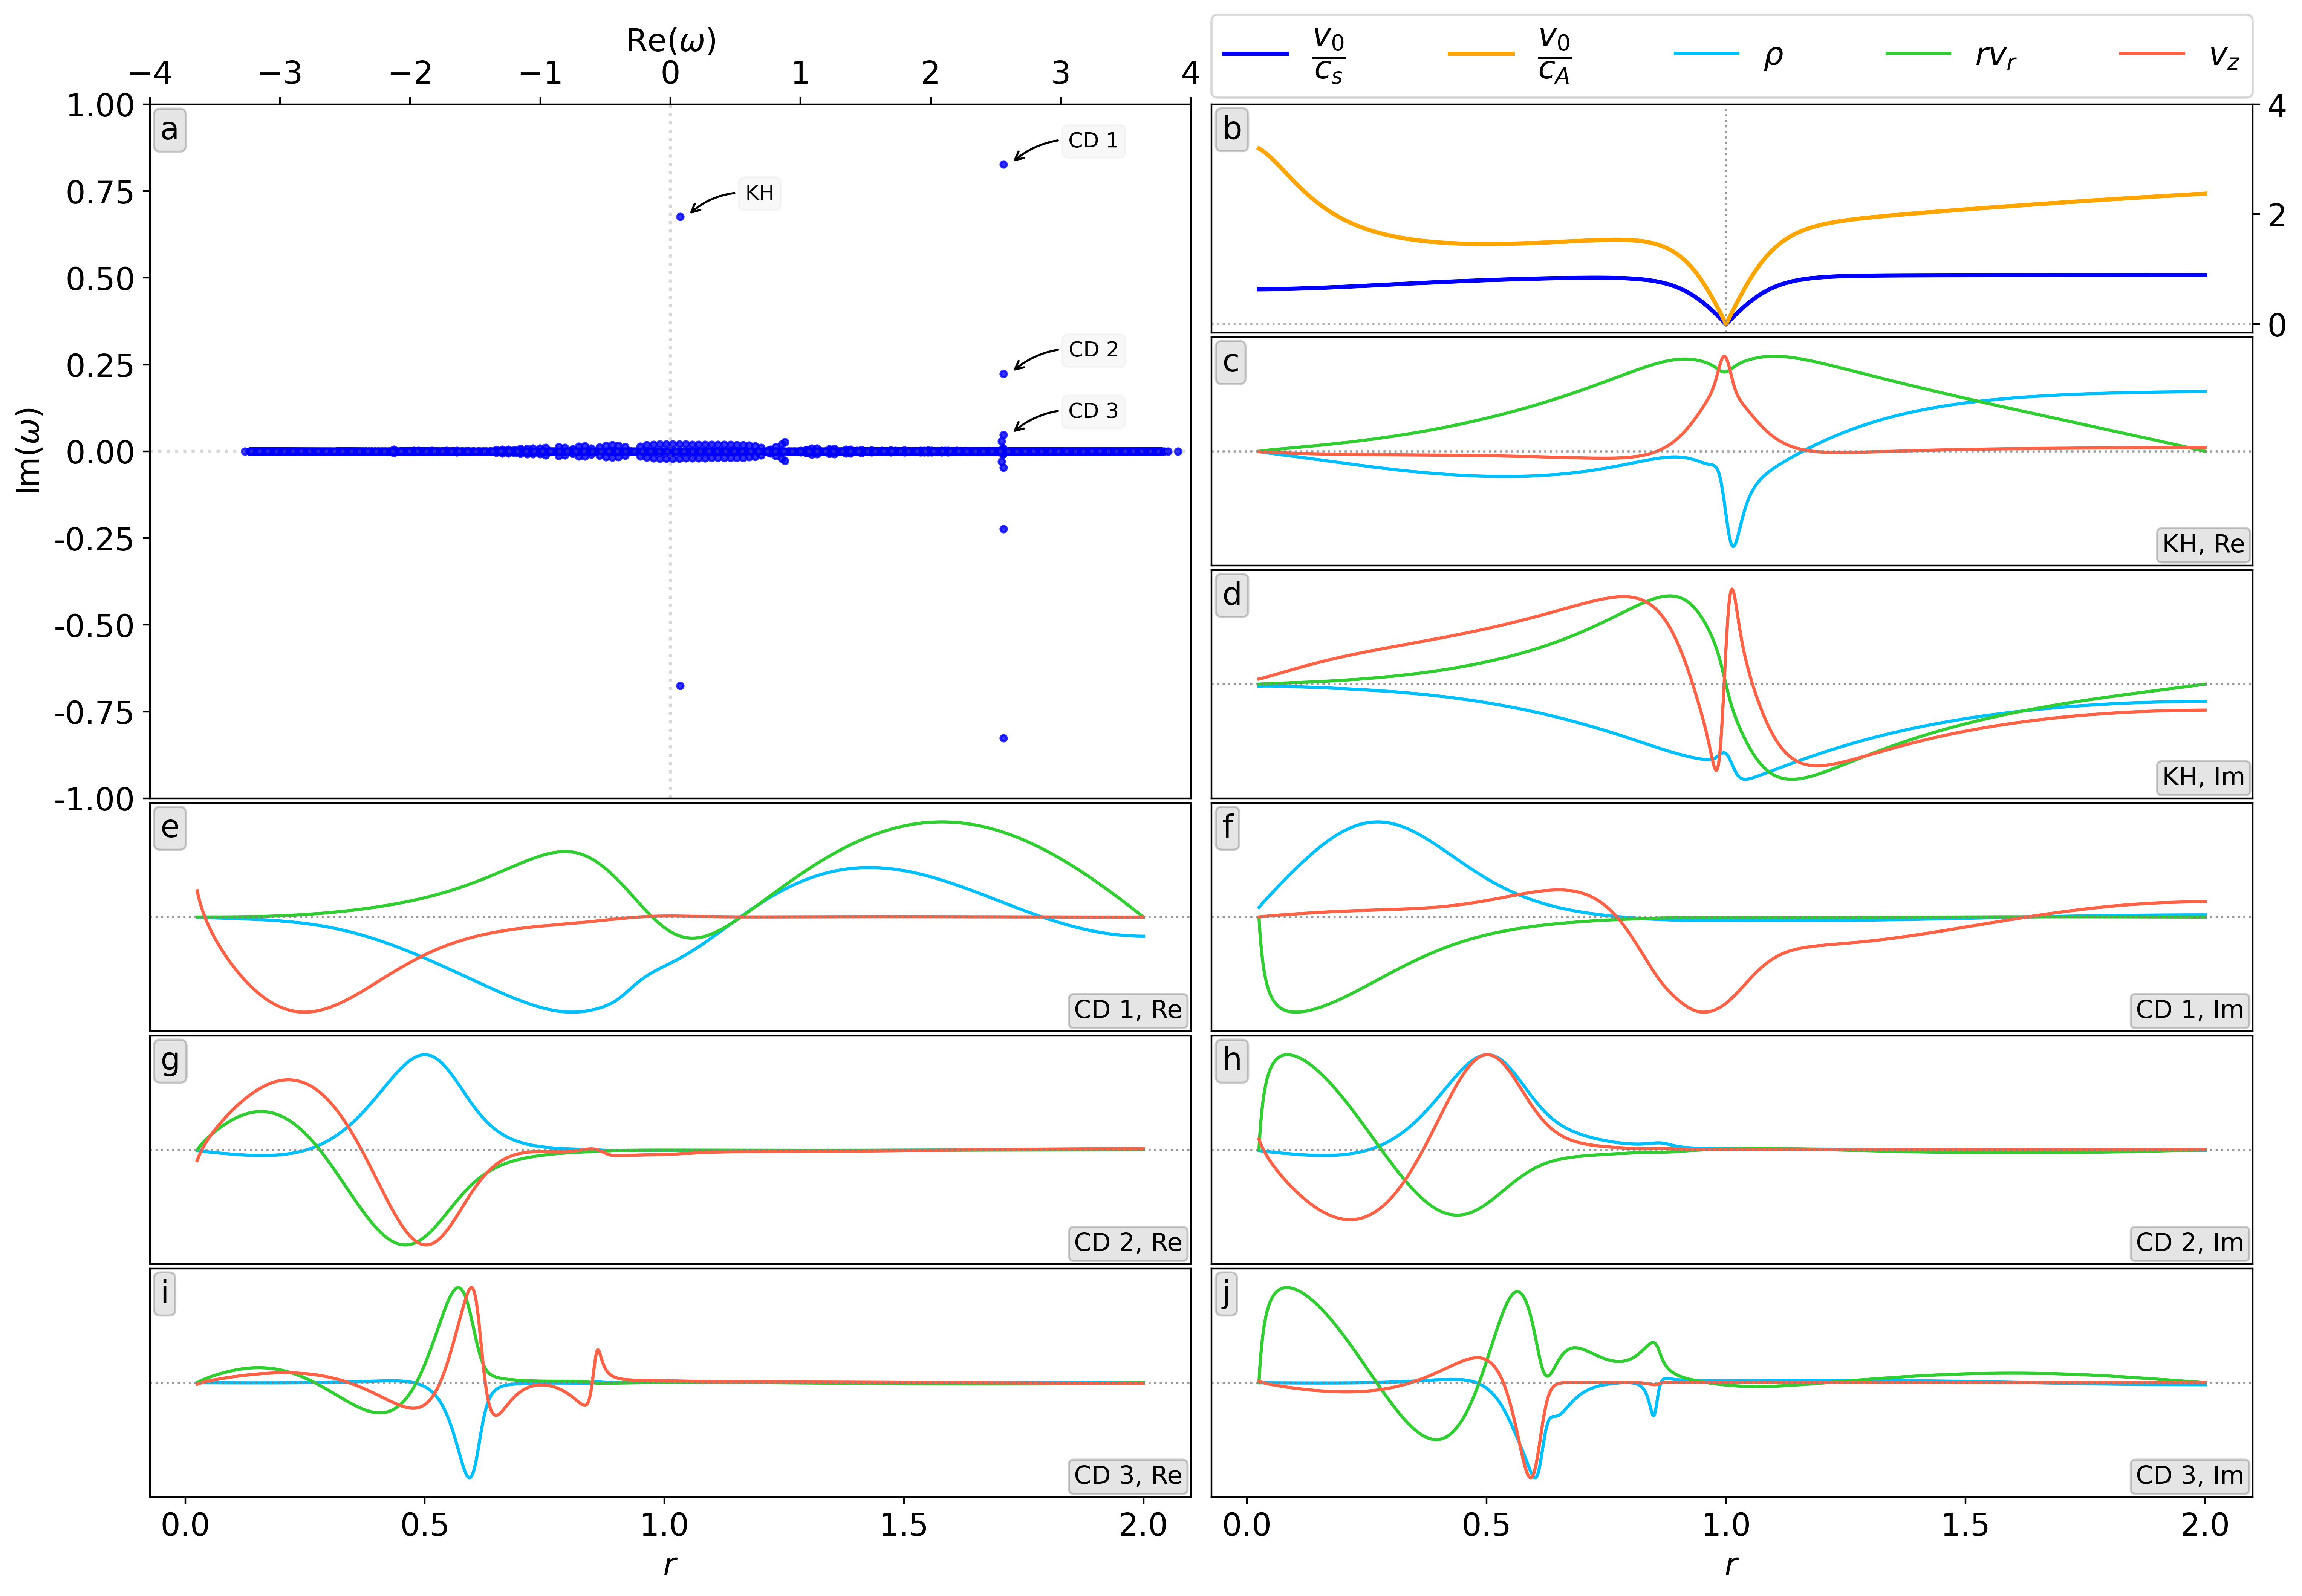
\includegraphics[width=\textwidth]{kh_cd.png}
  \caption{
    Panel \textbf{a}: MHD spectrum for the equilibrium configuration given in \eqref{eq: kh_cd_equilibrium}. The KH and CD instabilities are indicated on the panel. Panel \textbf{b}: sonic and Alfv\'enic Mach numbers; the other panels show the real and imaginary parts of the $\rho$ (blue), $r v_r$ (green) and $v_z$ (red) eigenfunctions, for the KH mode (Panels \textbf{c} and \textbf{d}), first CD mode (Panels \textbf{e}--\textbf{f}), second CD mode (Panels \textbf{g}--\textbf{h}), and third CD mode (Panels \textbf{i}--\textbf{j}).
  }
  \label{fig: kh_cd}
\end{figure}

Note that here, we are still in adiabatic conditions such that the up-down symmetry (relating to time reversal) is still present in the eigenfrequency plane, but the introduction of equilibrium flow caused left-right symmetry breaking between the forwards and backwards propagating modes. As pointed out in \citet{goedbloed2018_web1}, the study of MHD spectra of stationary (i.e. with flow) equilibria is still governed by two self-adjoint operators, but as seen in Figure \ref{fig: kh_cd}, modes can enter the complex plane at various locations (identified by the spectral web \citep{goedbloed2018_web2}). The correspondence with the original figure in \citet{baty2002} is one-to-one for the KH and CD modes, but here we have a lot more detail near the axes due to the (much) higher resolution employed. This resolution aspect will be further discussed in Section \ref{sec: convergence}.

\subsection{Suydam cluster modes}
Next we look at Suydam cluster modes in a cylindrical geometry, which arise from the presence of a Suydam surface in the equilibrium configuration, that is, a location where $\bk \cdot \bb_0 = 0$. Shear flow effects are included, and the equilibrium is given by
\begin{equation} \label{eq: suydam_equilibrium}
  \begin{gathered}
    \rho_0 = 1,
    \qquad
    v_{02} = 0,
    \qquad
    v_{03} = v_{0z}\left(1 - r^2\right),
    \qquad
    B_{02} = J_1(\alpha r), \\
    B_{03} = \sqrt{1 - P_1}J_0(\alpha r),
    \qquad
    p_0 = P_0 + \frac{1}{2}P_1 J_0^2(\alpha r),
  \end{gathered}
\end{equation}
where $\alpha = 2$, $P_0 = 0.05$, $P_1 = 0.1$, and $v_{0z} = 0.14$; the functions $J_0$ and $J_1$ denote the Bessel functions of the first kind. The wavenumbers were chosen to be $k_2 = m = 1$ and $k_3 = k = -1.2$, ensuring a Suydam surface at $r \approx 0.483$.

The spectrum is calculated using 501 gridpoints for $r \in [0, 1]$ and is shown in Figure \ref{fig: suydam_cluster}. The resulting locations of the various off-axis outer modes are in agreement with the results given in \citet{nijboer1997}. However, because this spectrum is calculated using a five times higher resolution, we have much more intricate detail near the Suydam surface, revealing even more off-axis modes (inset in Panel a). The top two panels on the right side of Figure \ref{fig: suydam_cluster} show the sonic and Alfv\'enic Mach numbers (Panel b), together with the $\bk \cdot \bb_0 = B_{02}k_2/r + B_{03}k_3$ and $\bk \cdot \bv_0 = v_{02}k_2/r + v_{03}k_3$ profiles as a function of radius (Panel c), respectively. The location of the Suydam surface at $r \approx 0.483$ is denoted with a red cross.

The bottom row of panels d--g shows the real part of the $\rho$ and $r v_r$ eigenfunctions, for the four modes annotated in Panel a with the location of the Suydam surface indicated with a vertical red line. $\omega_1$ en $\omega_3$ correspond to modes on the left side of the Suydam surface, the other two correspond to modes on the right side. All eigenfunctions shown here show the specific variation associated with their localised behaviour on the left side of the red dashed line, while it is vice versa for the other two modes. For visual purposes the horizontal axis in Panels e and f is different from the one in Panels c and d, because the former correspond to the next modes in the Suydam sequence, showing stronger radial variation. Note that the original Suydam criterion \citep{book_MHD} is related to static equilibria, the generalisation of these Suydam cluster criteria is presented in \citet{wang2004}.

\begin{figure}[t]
  \centering
  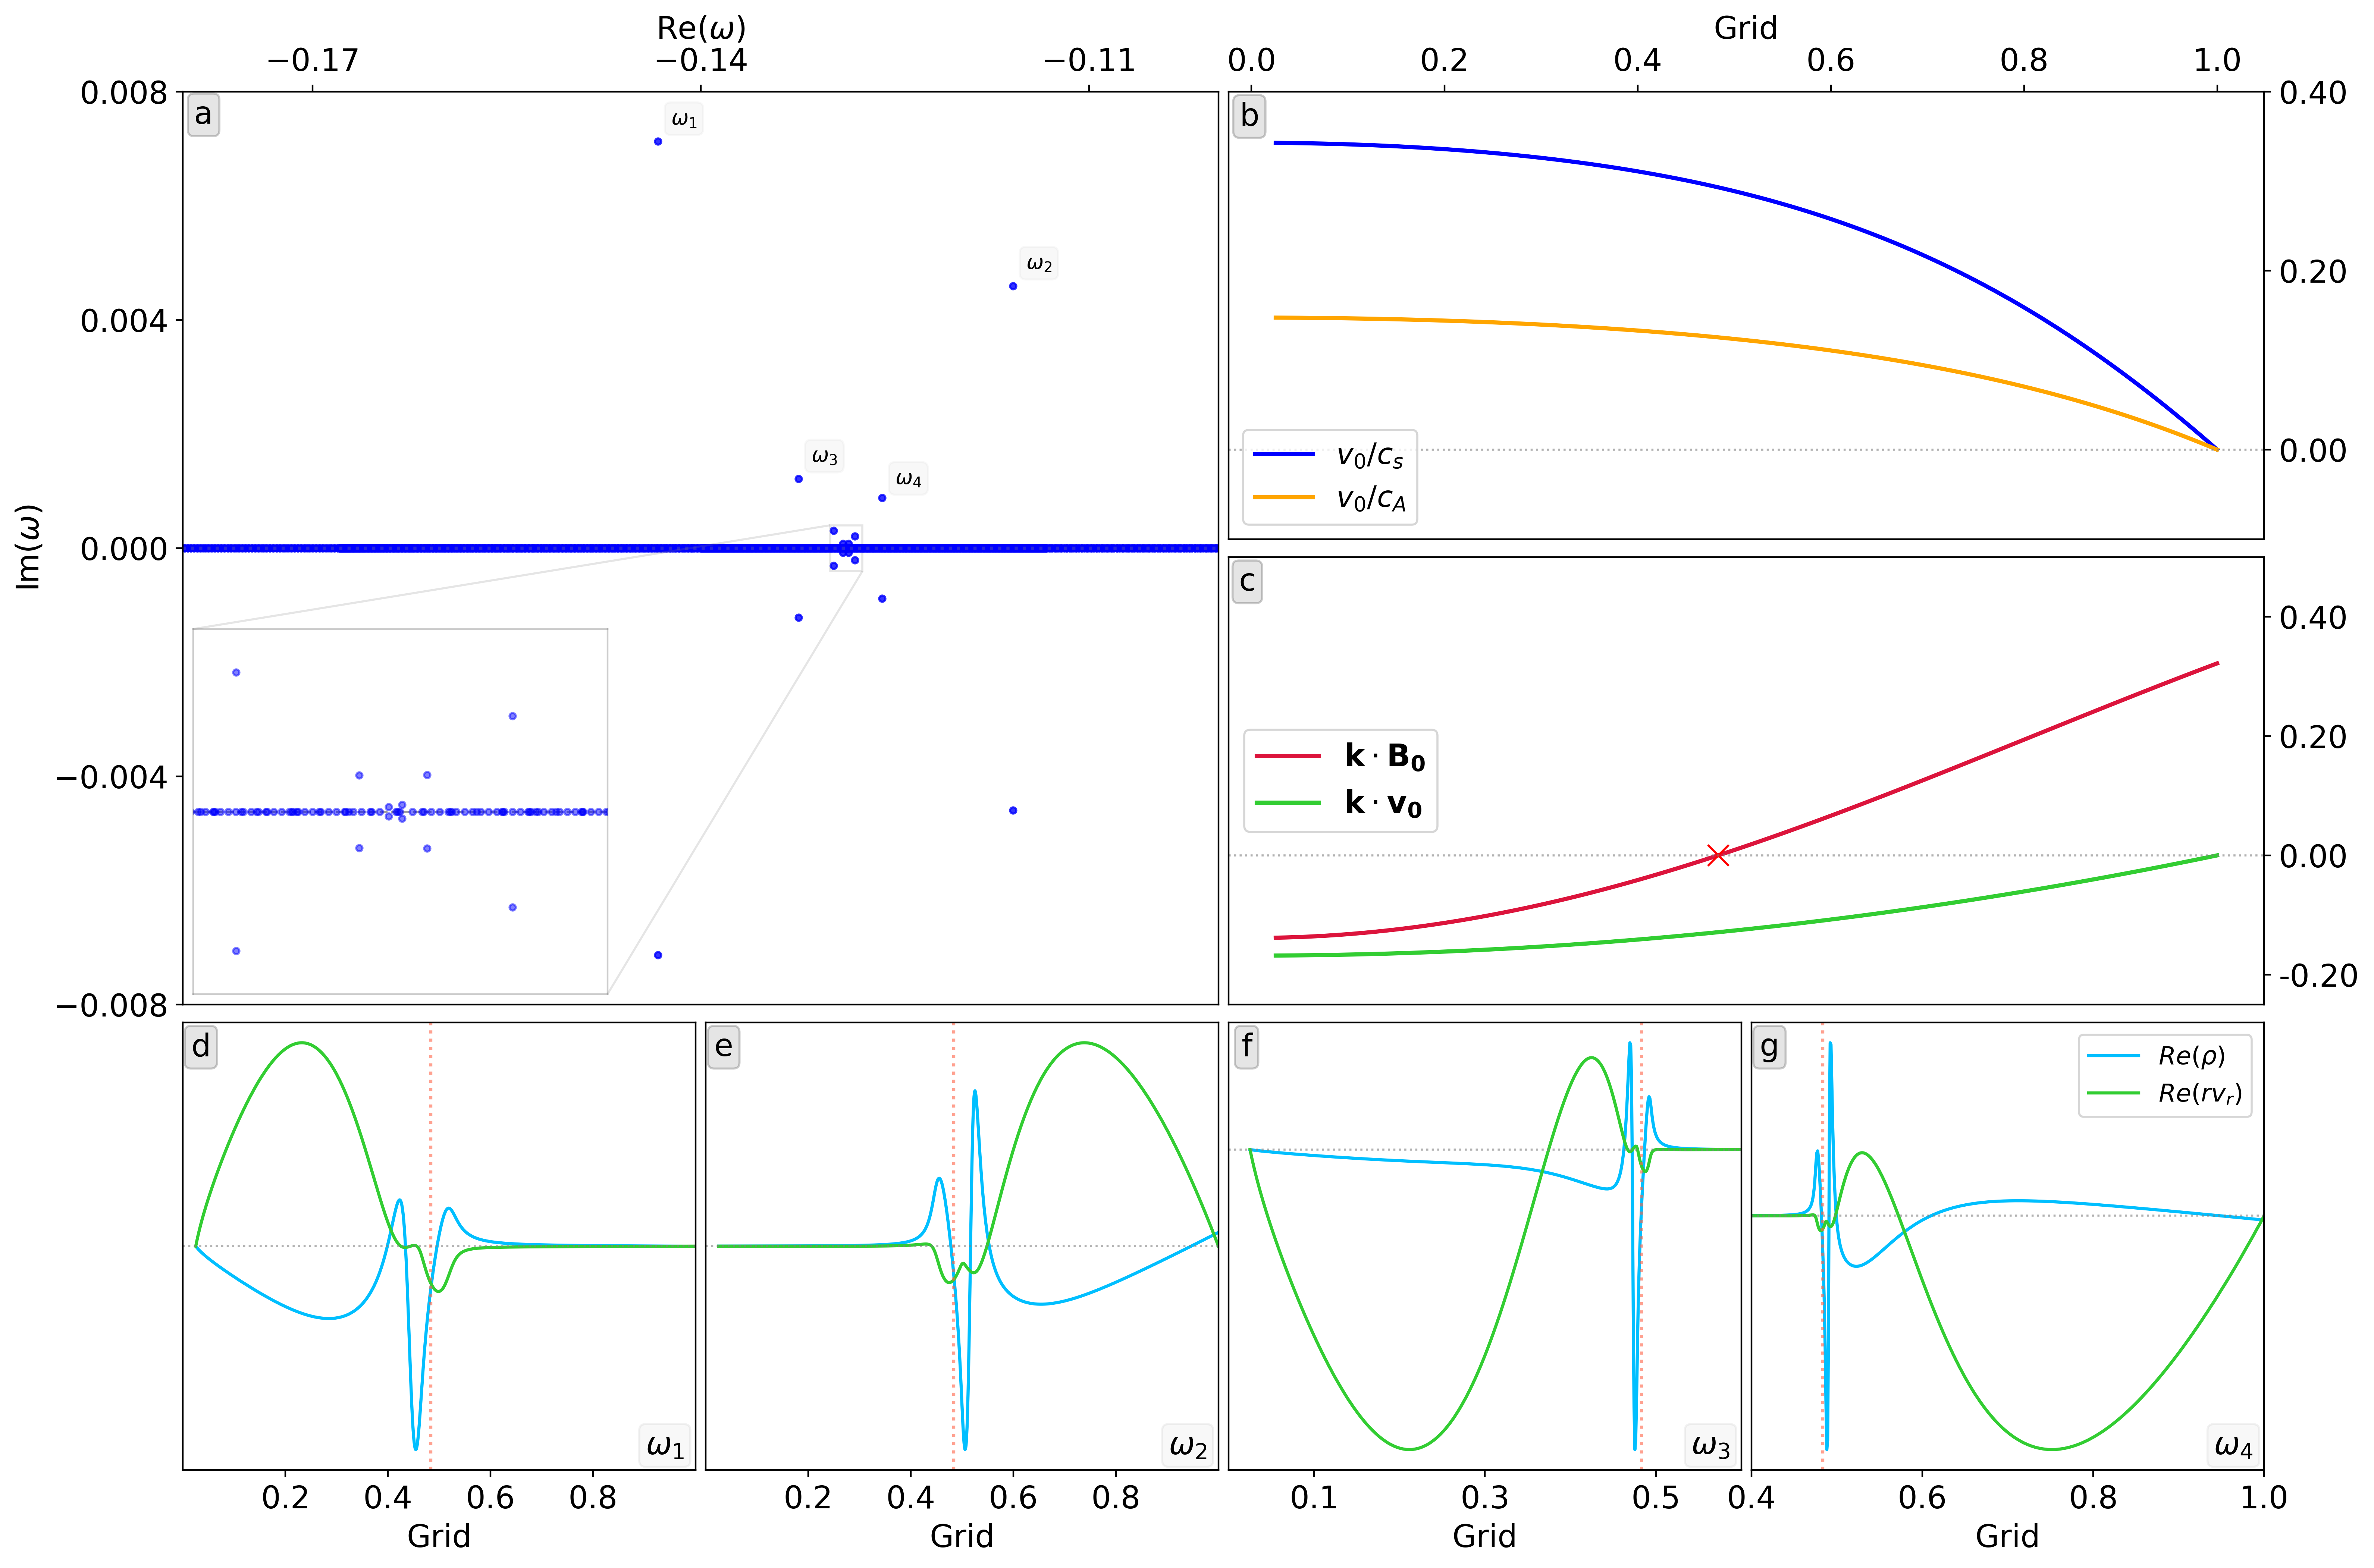
\includegraphics[width=\textwidth]{suydam_cluster.png}
  \caption{
    Panel \textbf{a}: Suydam cluster spectrum for the equilibrium given in \eqref{eq: suydam_equilibrium}. Inset: zoom-in near the Suydam surface, revealing more detail. Panel \textbf{b} depicts the sonic and Alfv\'enic Mach numbers as a function of radius, Panel \textbf{c} shows the $\bk \cdot \bb_0$ and $\bk \cdot \bv_0$ curves where the red cross denotes the Suydam surface. The bottom row of panels shows the real part of the $\rho$ and $r v_r$ eigenfunctions, for the four modes in the Suydam sequence annotated in Panel \textbf{a}. The dotted red line denotes the location of the Suydam surface.
  }
  \label{fig: suydam_cluster}
\end{figure}



\section{Resistive, Cartesian cases}
All cases discussed up to now handles an adiabatic equilibrium configuration with or without the inclusion of flow. The up-down symmetry of all the MHD spectra shown so far is perfectly maintained, related to the fact that these cases are in essence time-reversible. Every instability (or overstability in the case of flow) has a damped counterpart. We now move on to include additional effects, that is, we now calculate spectra for time-irreversible cases, where either resistivity or non-adiabatic effects enter, which will break the up-down symmetry. We first focus on the inclusion of resistivity.


\subsection{Resistive homogeneous plasmas}
To start with we take a look at the simplest configuration, that is, a homogeneous plasma in a Cartesian geometry with resistivity included. The uniform equilibrium is given by
\begin{equation} \label{eq: resistive_homo_equilibrium}
  \rho_0 = 1,
  \qquad
  B_{02} = 0,
  \qquad
  B_{03} = 1,
  \qquad
  T_0 = \frac{1}{2}\beta B_0^2
\end{equation}
where we take a plasma beta of $\beta = 0.25$, $k_2 = k_y = 0$, $k_3 = k_z = 1$, and $x \in [0, 1]$. The value for the resistivity is assumed to be constant and given by $\eta = 10^{-3}$, as described in \citet{book_MHD}. This spectrum is calculated using 1001 gridpoints; the result is shown in Figure \ref{fig: resistive_homo}. In ideal MHD the fast modes form a Sturmian sequence (that is, the oscillation of the eigenfrequencies increases then the number of modes increases, which in turn implies a larger real part of $\omega$) of stable fast magnetoacoustic waves with frequencies accumulating to infinite frequency (related to the $p$ modes in our stratified example). The slow modes have an anti-Sturmian sequence toward their accumulation point (in essence the collapsed slow continuum) and the Alfv\'en modes are degenerate \citep{book_MHD}. When resistivity is included, the fast modes become damped and the Alfv\'en and slow modes trace out semicircles on the bottom-half of the complex plane. The semicircles and initial fast-mode sequence shown in Figure \ref{fig: resistive_homo} are in perfect agreement with the spectrum depicted in \citet[Figure 14.6]{book_MHD}. These semicircles can be quantified analytically; their radius does not depend on resistivity. The magnetic Reynolds number, calculated as $\magneticreynolds = (x_1 - x_0)\alfvenspeed / \eta$, is equal to 1000.

Due to the rather extreme resolution employed here, we trace much further into the fast-mode sequence, where we see something interesting: the fast modes appear on curves that loop around, breaking the purely Sturmian behaviour for a moment, after which they continue again toward infinity. This implies that initially, the fast modes become more damped at higher mode frequencies up to a certain turning point at which they achieve maximal damping (the bottom of the loop). After passing this turning point, the oscillation frequency of the modes increases again and the damping frequency seems to converge toward one single value.

Of course, the strong damping for the fast modes as we go further into the fast-mode sequence must have consequences for the original uniform (ideal) equilibrium state. In what follows, we will adopt the common practice of computing resistive MHD spectra about an ideal MHD state, which itself will evolve when resistivity is acting. This is directly related to the discussion on the equilibrium background in Section \ref{ss: equilibrium conditions} when resistivity is taken into account.

\begin{figure}[t]
  \centering
  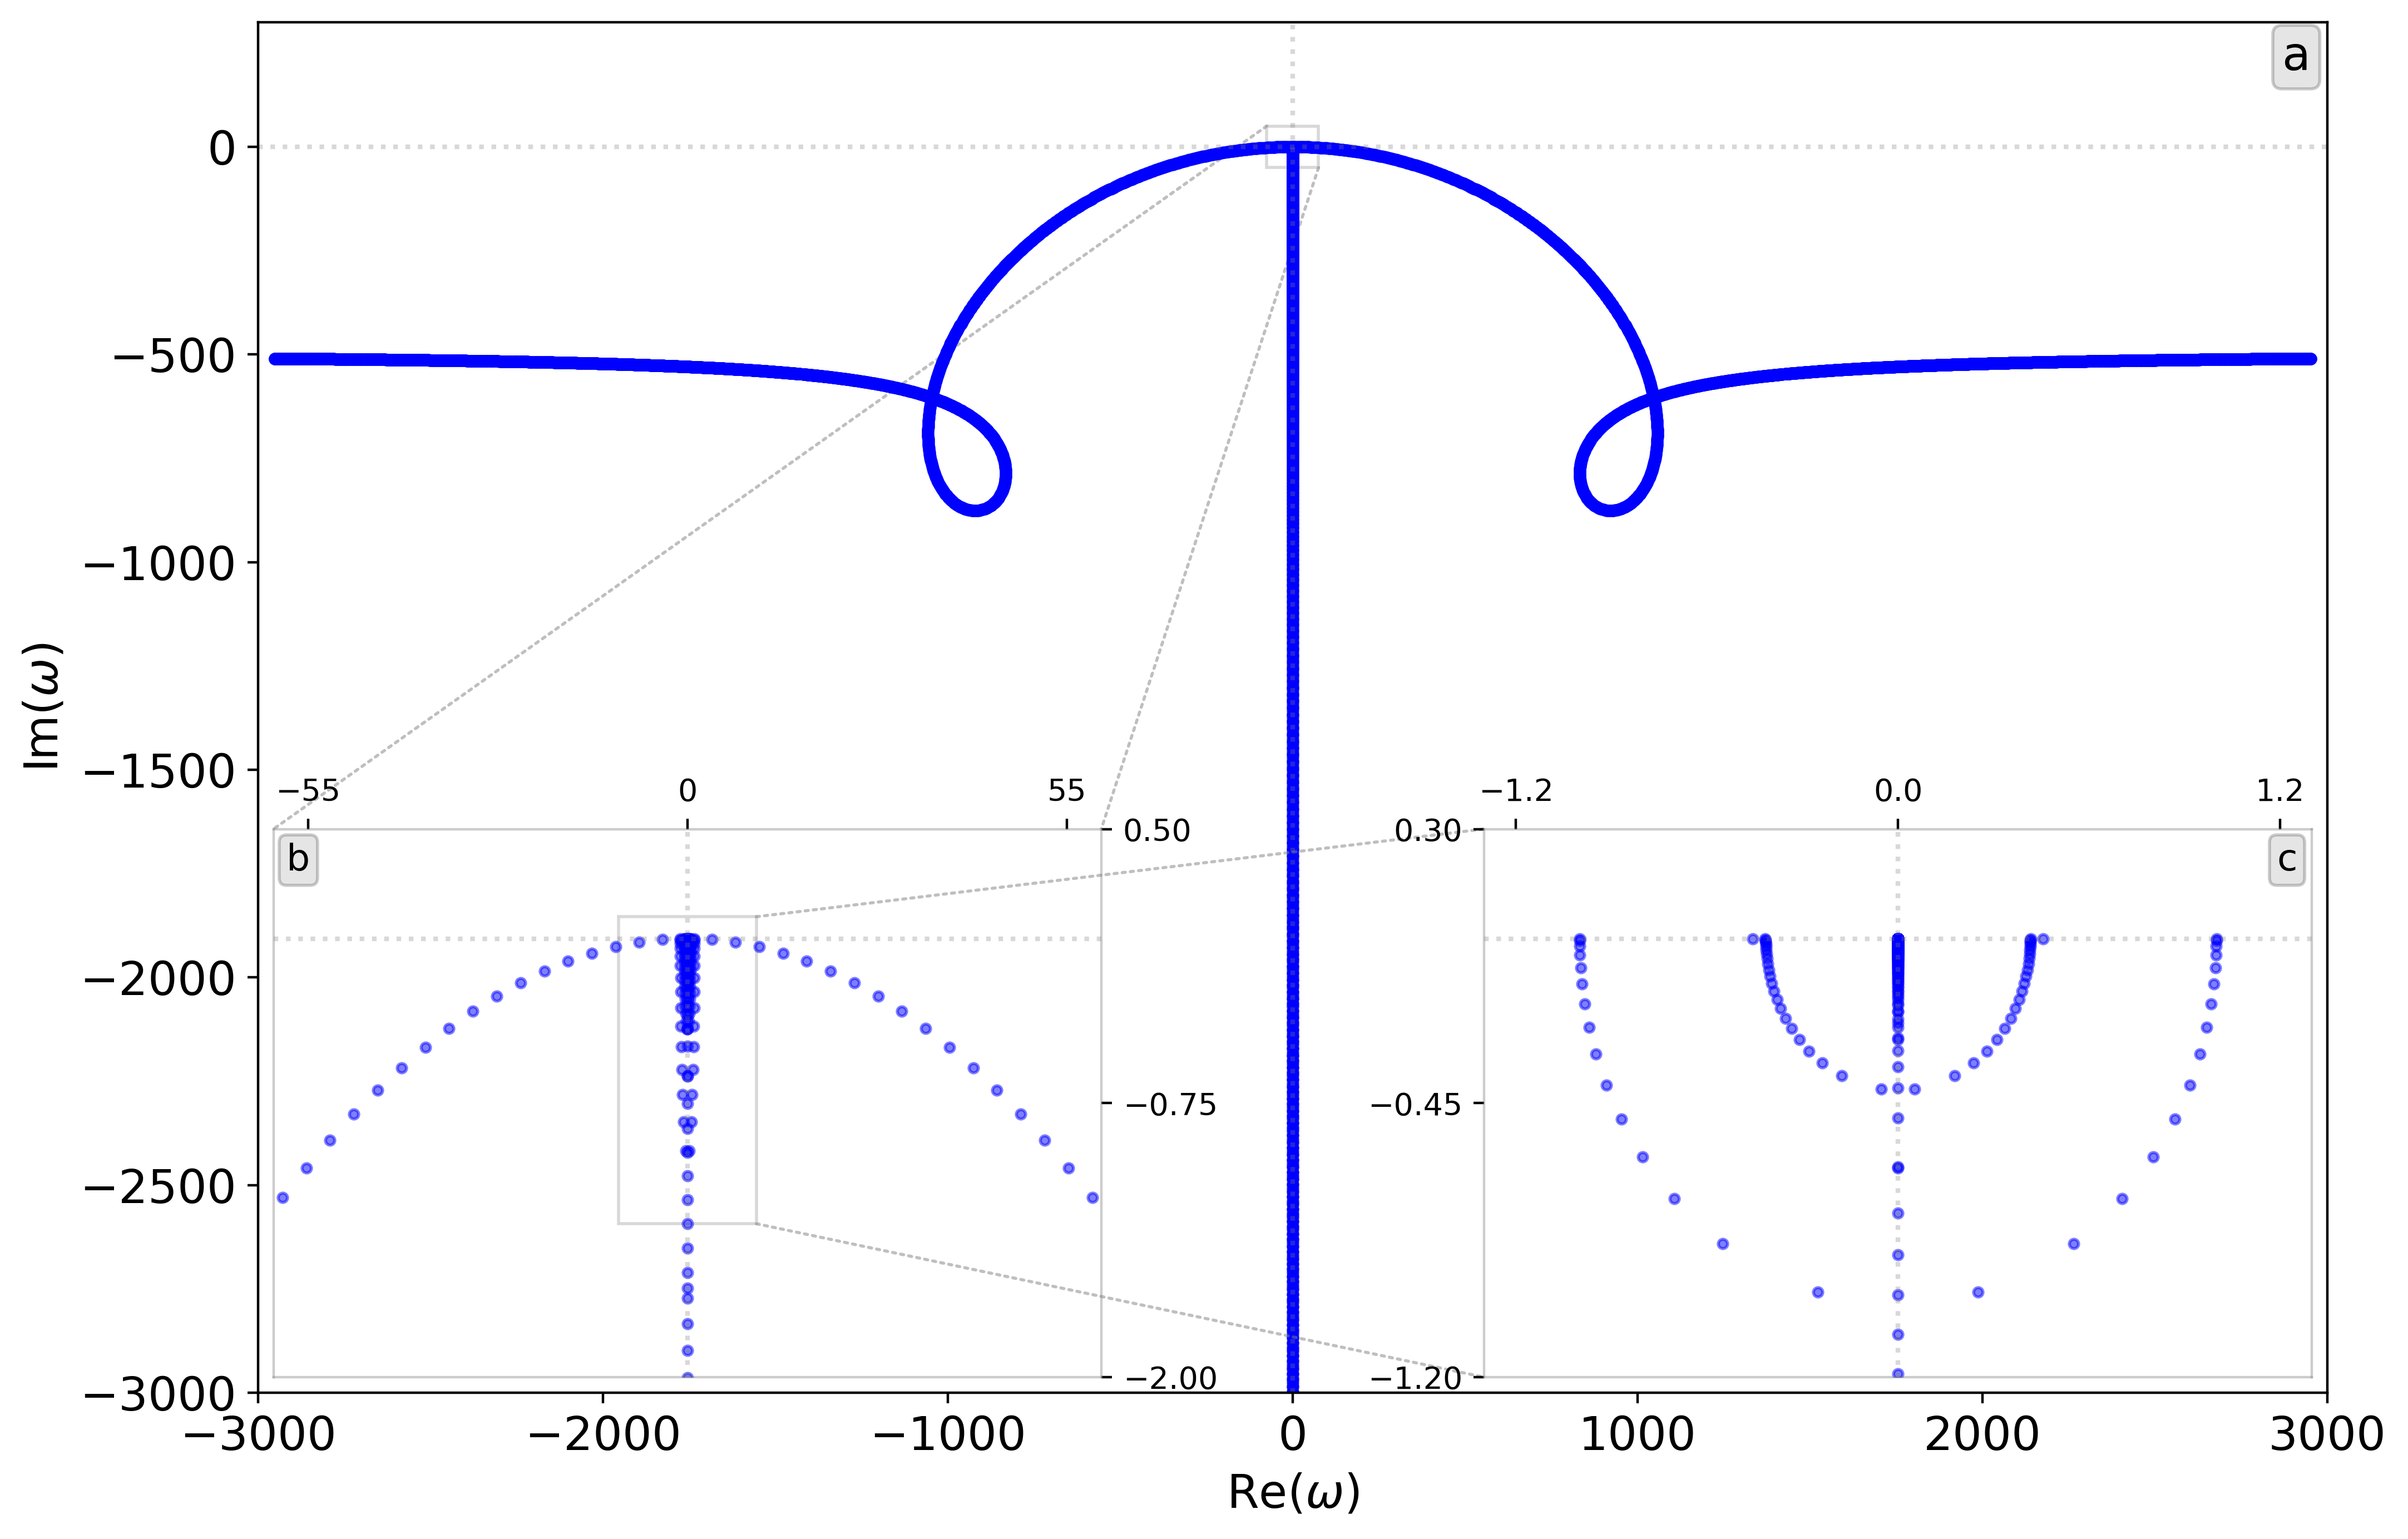
\includegraphics[width=\textwidth]{resistive_homo.png}
  \caption{
    Panel \textbf{a}: spectrum for a homogeneous medium with constant resistivity. Panel \textbf{b} zooms in near the origin, showing the start of the fast-mode sequence. Panel \textbf{c} zooms in further, revealing the semicircles traced out by the Alfv\'en and slow modes (outer and inner semicircles, respectively).
  }
  \label{fig: resistive_homo}
\end{figure}


\subsection{Quasi-modes in resistive MHD}
We now turn to a nonadiabatic case, where resistivity is important. We will compute the resistive MHD spectrum for a case where the equilibrium varies across an interface, which gives rise to so-called quasi-modes. These are essentially surface waves undergoing damping, due to the fact that the global quasi-mode overlaps in frequency with the continuum range, causing resonant absorption. Quasi-modes are quite important in solar physics, as they can be indirectly related to the coronal heating problem as discussed in, for example, \citet{poedts1989} and \citet{poedts1991}. As a side note it should be remarked that in resistive MHD transient growth may potentially be significant for the linear evolution of non-ideal systems \citep{mactaggart2018}, but we will not consider that here.

A detailed analytical treatment of quasi-modes including theoretical growth rates is given in \citet{book_priest}, where they start from an inhomogeneous layer of width $l$ connecting two regions of uniform plasma. This can be reproduced by introducing a linear density profile between two homogeneous regions in a Cartesian geometry, however, this would mean that the density derivative shows rather strong discontinuities near the edges of the transition layer. Similar to \citet{ruderman2002} we therefore opt for a smooth profile by introducing a sine dependence such that

\begin{equation}
  \rho_0(x) =
  \begin{cases}
    \rho_1 &\text{if}~x_0 \leq x < s - \dfrac{1}{2}l, \\
    \dfrac{1}{2}\rho_1\left[
      1 + \dfrac{\rho_2}{\rho_1} - \left(1 - \dfrac{\rho_2}{\rho_1}\right)\sin\left(\dfrac{\pi(x - s)}{l}\right)
    \right] &\text{if}~s - \dfrac{1}{2}l \leq x \leq s + \dfrac{1}{2}l, \\
    \rho_2 &\text{if}~s + \dfrac{1}{2}l < x \leq x_1,
  \end{cases}
\end{equation}
where $s$ denotes the midpoint between $x_0$ and $x_1$, representing the left and right edges of the Cartesian grid, respectively, and equal to $0$ and $1$ such that $s = 0.5$. The width of the transition region $l = 0.1$ is taken to be small as to reduce the influence of the walls. If $l \rightarrow 0$, the inhomogeneous region disappears, and we simply have a discontinuous jump in the plasma. Furthermore, we take $\rho_1 = 0.9$, $\rho_2 = 0.1$, $B_{02} = 0$, $B_{03}$ = 1, and $T_0 = 0$. The magnetic field is unidirectional along the $z$-axis, and setting the temperature (and thus pressure) to zero provides an additional test on the handling of zero rows in the matrix. This zero-temperature case is frequently encountered in fully nonlinear MHD simulations which artificially adopt a zero plasma beta. It has as an important consequence that the slow continuum collapses to marginal frequency, eliminating many interesting modes from the spectrum. Additionally, we adopt wavenumbers $k_3 = 0.05$ and $k_2 = 1$, such that $k_3 \ll k_2$. As discussed in \citet{book_priest}, the quasi-modes are damped, such that they move away from the real eigenfrequency axis with complex eigenvalues $\omega = \omega_\text{R} + \icomplex \omega_\text{I}$ given by
\begin{equation} \label{eq: quasimode}
  \omega_\text{R} = \pm \sqrt{\frac{\rho_1 \omega_\text{A1}^2 + \rho_2 \omega_\text{A2}^2}{\rho_1 + \rho_2}},
  \qquad
  \omega_\text{I} = -\frac{\pi k_z l \left(\omega_\text{A2}^2 - \omega_\text{A1}^2\right)}{8\omega_\text{R}},
\end{equation}
with $\omega_\text{A}^2 = k_z^2 \alfvenspeed^2$. This analytic result originates from a complex analysis of the linearised initial value problem. However, there is one caveat: it is impossible to obtain complex eigenvalues away from the real or imaginary axis in an ideal plasma, due to the matrix operator being Hermitian in ideal MHD. Because the (ideal) quasi-mode is damped, we therefore include a (small) value for the resistivity, $\eta = 10^{-4}$, which is sufficient to make the matrix operator non-Hermitian and allows for complex eigenvalues away from the horizontal axis.

\begin{figure}[t]
  \centering
  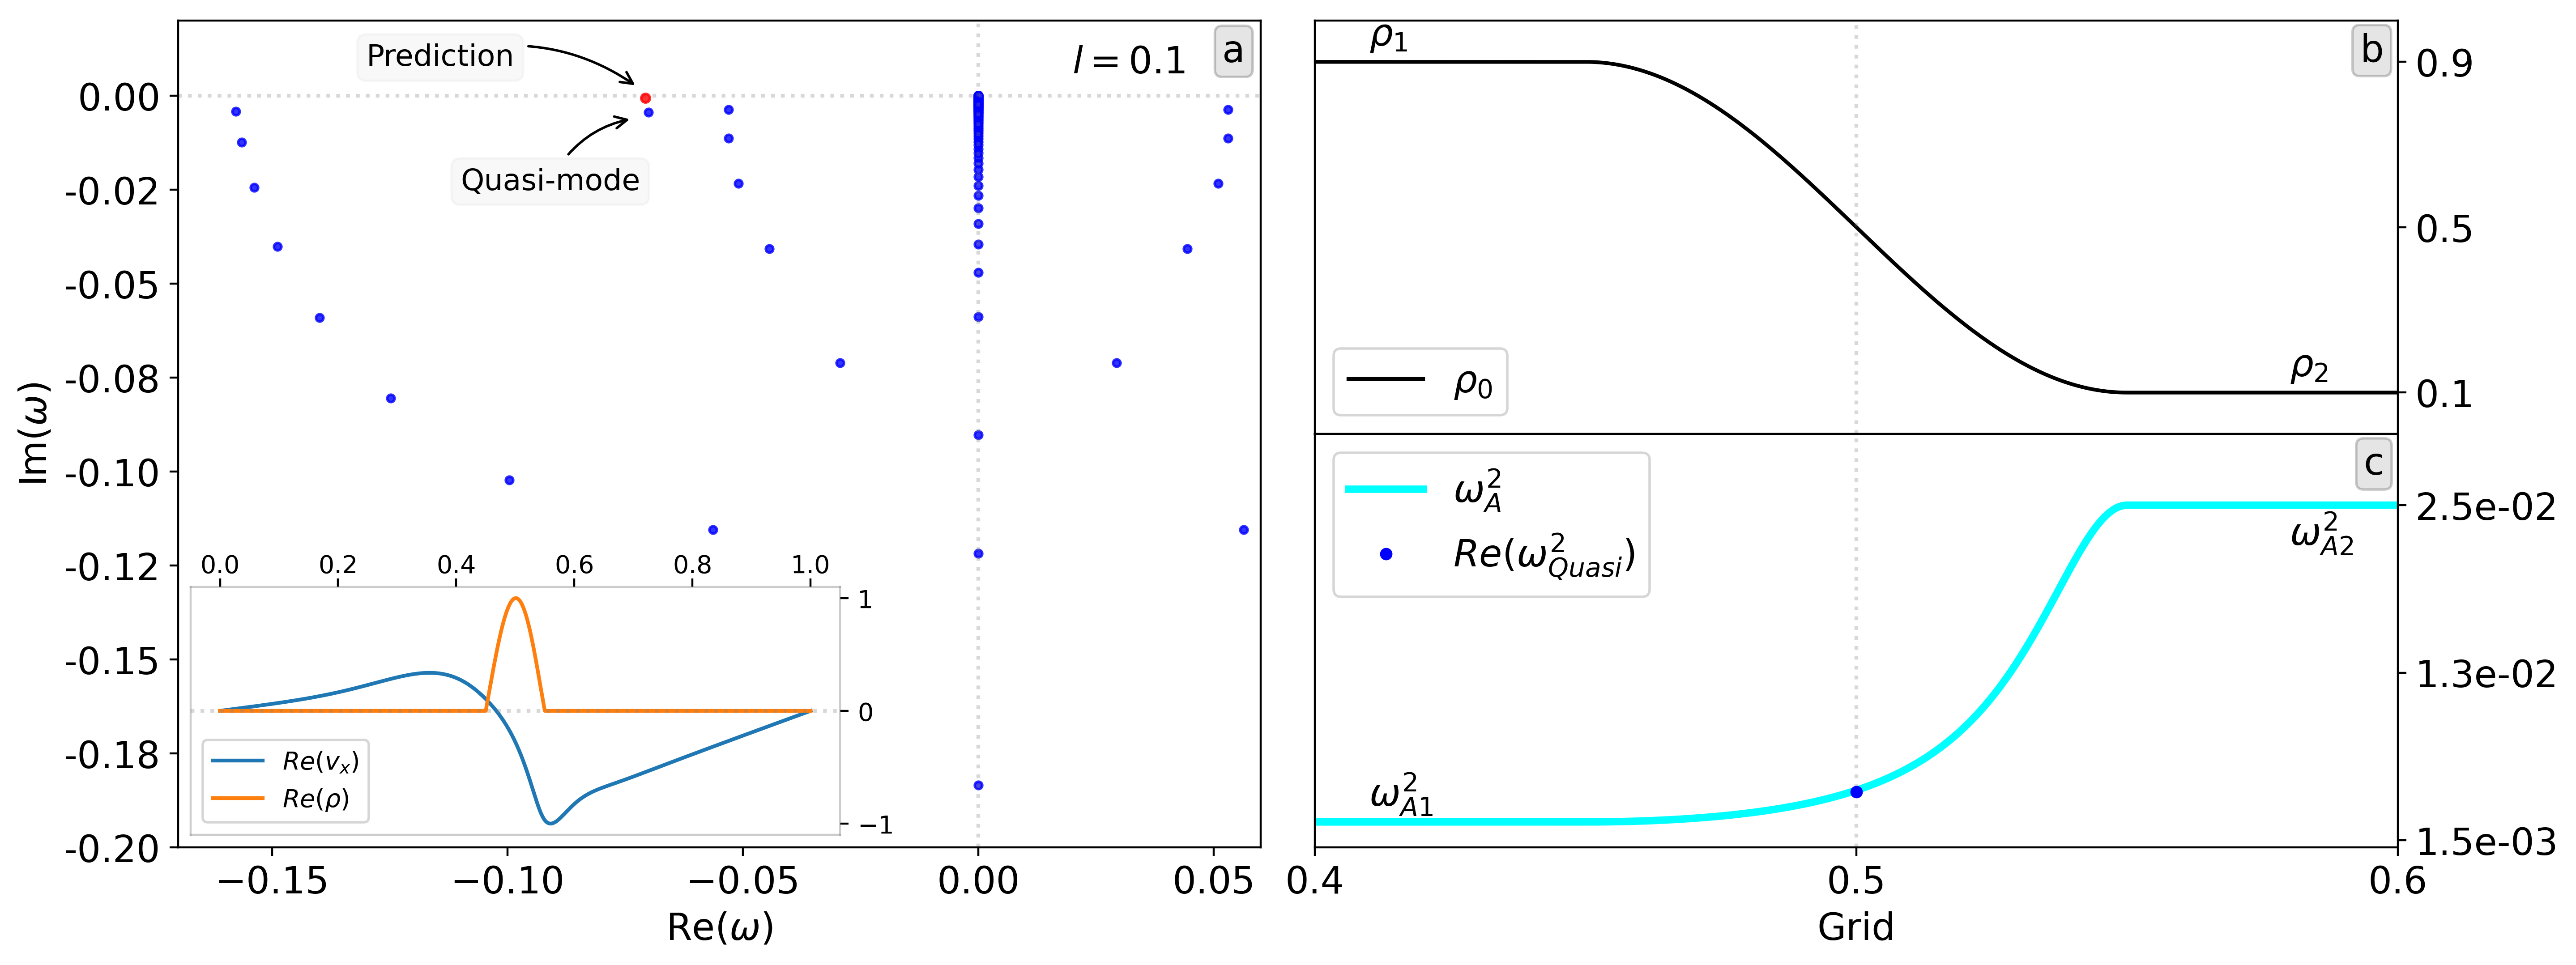
\includegraphics[width=\textwidth]{quasimodes.png}
  \caption{
    Panel \textbf{a}: part of the MHD spectrum containing the quasi-mode, the red dot denotes the theoretical prediction of Equation \eqref{eq: quasimode}. Panels \textbf{b} and \textbf{c} show plots of the sinusoidal density profile and Alfv\'en frequency as a function of the grid, respectively. Note that these two panels only show part of the grid, near the transition region. The inset shows the real part of the $v_x$ (orange) and $\rho$ (blue) normalised eigenfunctions associated with the quasi-mode. The blue dot in Panel \textbf{c} denotes the squared quasi-mode frequency, matching the squared Alfv\'en frequency at $x = 0.5$. The vertical dotted line denotes the middle of the grid.
  }
  \label{fig: quasimodes}
\end{figure}


The magnetic Reynolds number in this case varies between $\magneticreynolds \approx 10^4$ and $\magneticreynolds \approx 3 \times 10^4$. Figure \ref{fig: quasimodes} shows the MHD spectrum in Panel a, for 501 gridpoints, with the theoretical prediction for the global quasi-mode location annotated with a red dot. The actual quasi-mode is also denoted in the figure and is slightly more damped than its theoretical counterpart. This is to be expected, because the inclusion of resistivity imposed additional damping on the eigenvalues, shifting them downwards. It should be noted that increasing the width $l$ of the transition layer moves the quasi-mode farther down and to the right in the figure, such that it eventually merges with the damped modes found on the branch immediately to its right. This phenomenon, where the quasi-modes merge with the resistive branches, is discussed in more detail in \citet{vandoorsselaere2007}. The inset in Panel a depicts the $\rho$ (blue) and $v_x$ (orange) eigenfunctions associated with the quasi-mode, showing localised variation near the transition region as expected. Note that the spectrum as shown in Figure \ref{fig: quasimodes}, left Panel a, is still left-right symmetric, but that resistivity has broken the up-down symmetry, with all modes here found in the stable (damped) half plane.


\subsection{Resistive tearing modes}
Now we move on to an inhomogeneous medium with the inclusion of resistivity and an optional linear flow profile, discussed in \citet{book_MHD}. The geometry is Cartesian, with $x \in [-0.5, 0.5]$ and an equilibrium configuration given by
\begin{equation} \label{eq: resistive_tearing}
  \begin{gathered}
    \rho_0 = 1,
    \qquad
    B_{02} = \sin(\alpha x),
    \qquad
    B_{03} = \cos(\alpha x), \\
    T_0 = \frac{1}{2}\beta B_0^2,
    \qquad
    v_{02} = \mathcal{V}x,
    \qquad
    v_{03} = 0,
  \end{gathered}
\end{equation}
where $k_3 = k_z = 0$, $\beta = 0.15$, and $\alpha = 4.73884$, with a constant resistivity value of $\eta = 10^{-4}$. The magnetic configuration chosen here is a linear force-free field with shear, where $\alpha$ is the proportionality constant between the current and magnetic field, that is, $\boldsymbol{j_0} = \alpha \bb_0$. This specific choice of parameters violates the tearing mode stability criterion \citep{book_MHD}, which results in an isolated, unstable tearing mode. Spectra are calculated both for $\mathcal{V} = 0$ (no flow) and $\mathcal{V} = 0.15$, the inclusion of a linear velocity profile in the latter case introduces a Doppler shift in the slow and Alfv\'en continua, and the results are shown for 501 gridpoints in Figure \ref{fig: resistive_tearing}. Panels a and b show spectra for
$\mathcal{V} = 0$, $k_2 = k_y = 0.49$ (no flow) and $\mathcal{V} = 0.15$, $k_y = 1.5$ (linear flow profile), respectively, revealing the intricate behaviour of the damped slow and Alfv\'en sequences. The purely imaginary unstable tearing mode is annotated with an arrow. The resistivity $\eta$ is equal to $10^{-4}$ for both cases, yielding a magnetic Reynolds number of $\magneticreynolds \approx 10^4$. These results are in perfect agreement with the original spectra depicted in \citet[Figures 14.7--14.9]{book_MHD}. Note that these cases still have left-right symmetry maintained, despite the presence of equilibrium flow. However, this is purely because the flow profile and domain happen to be chosen in a symmetric way, such that forward and backward modes behave symmetrically.

\begin{figure}[t]
  \centering
  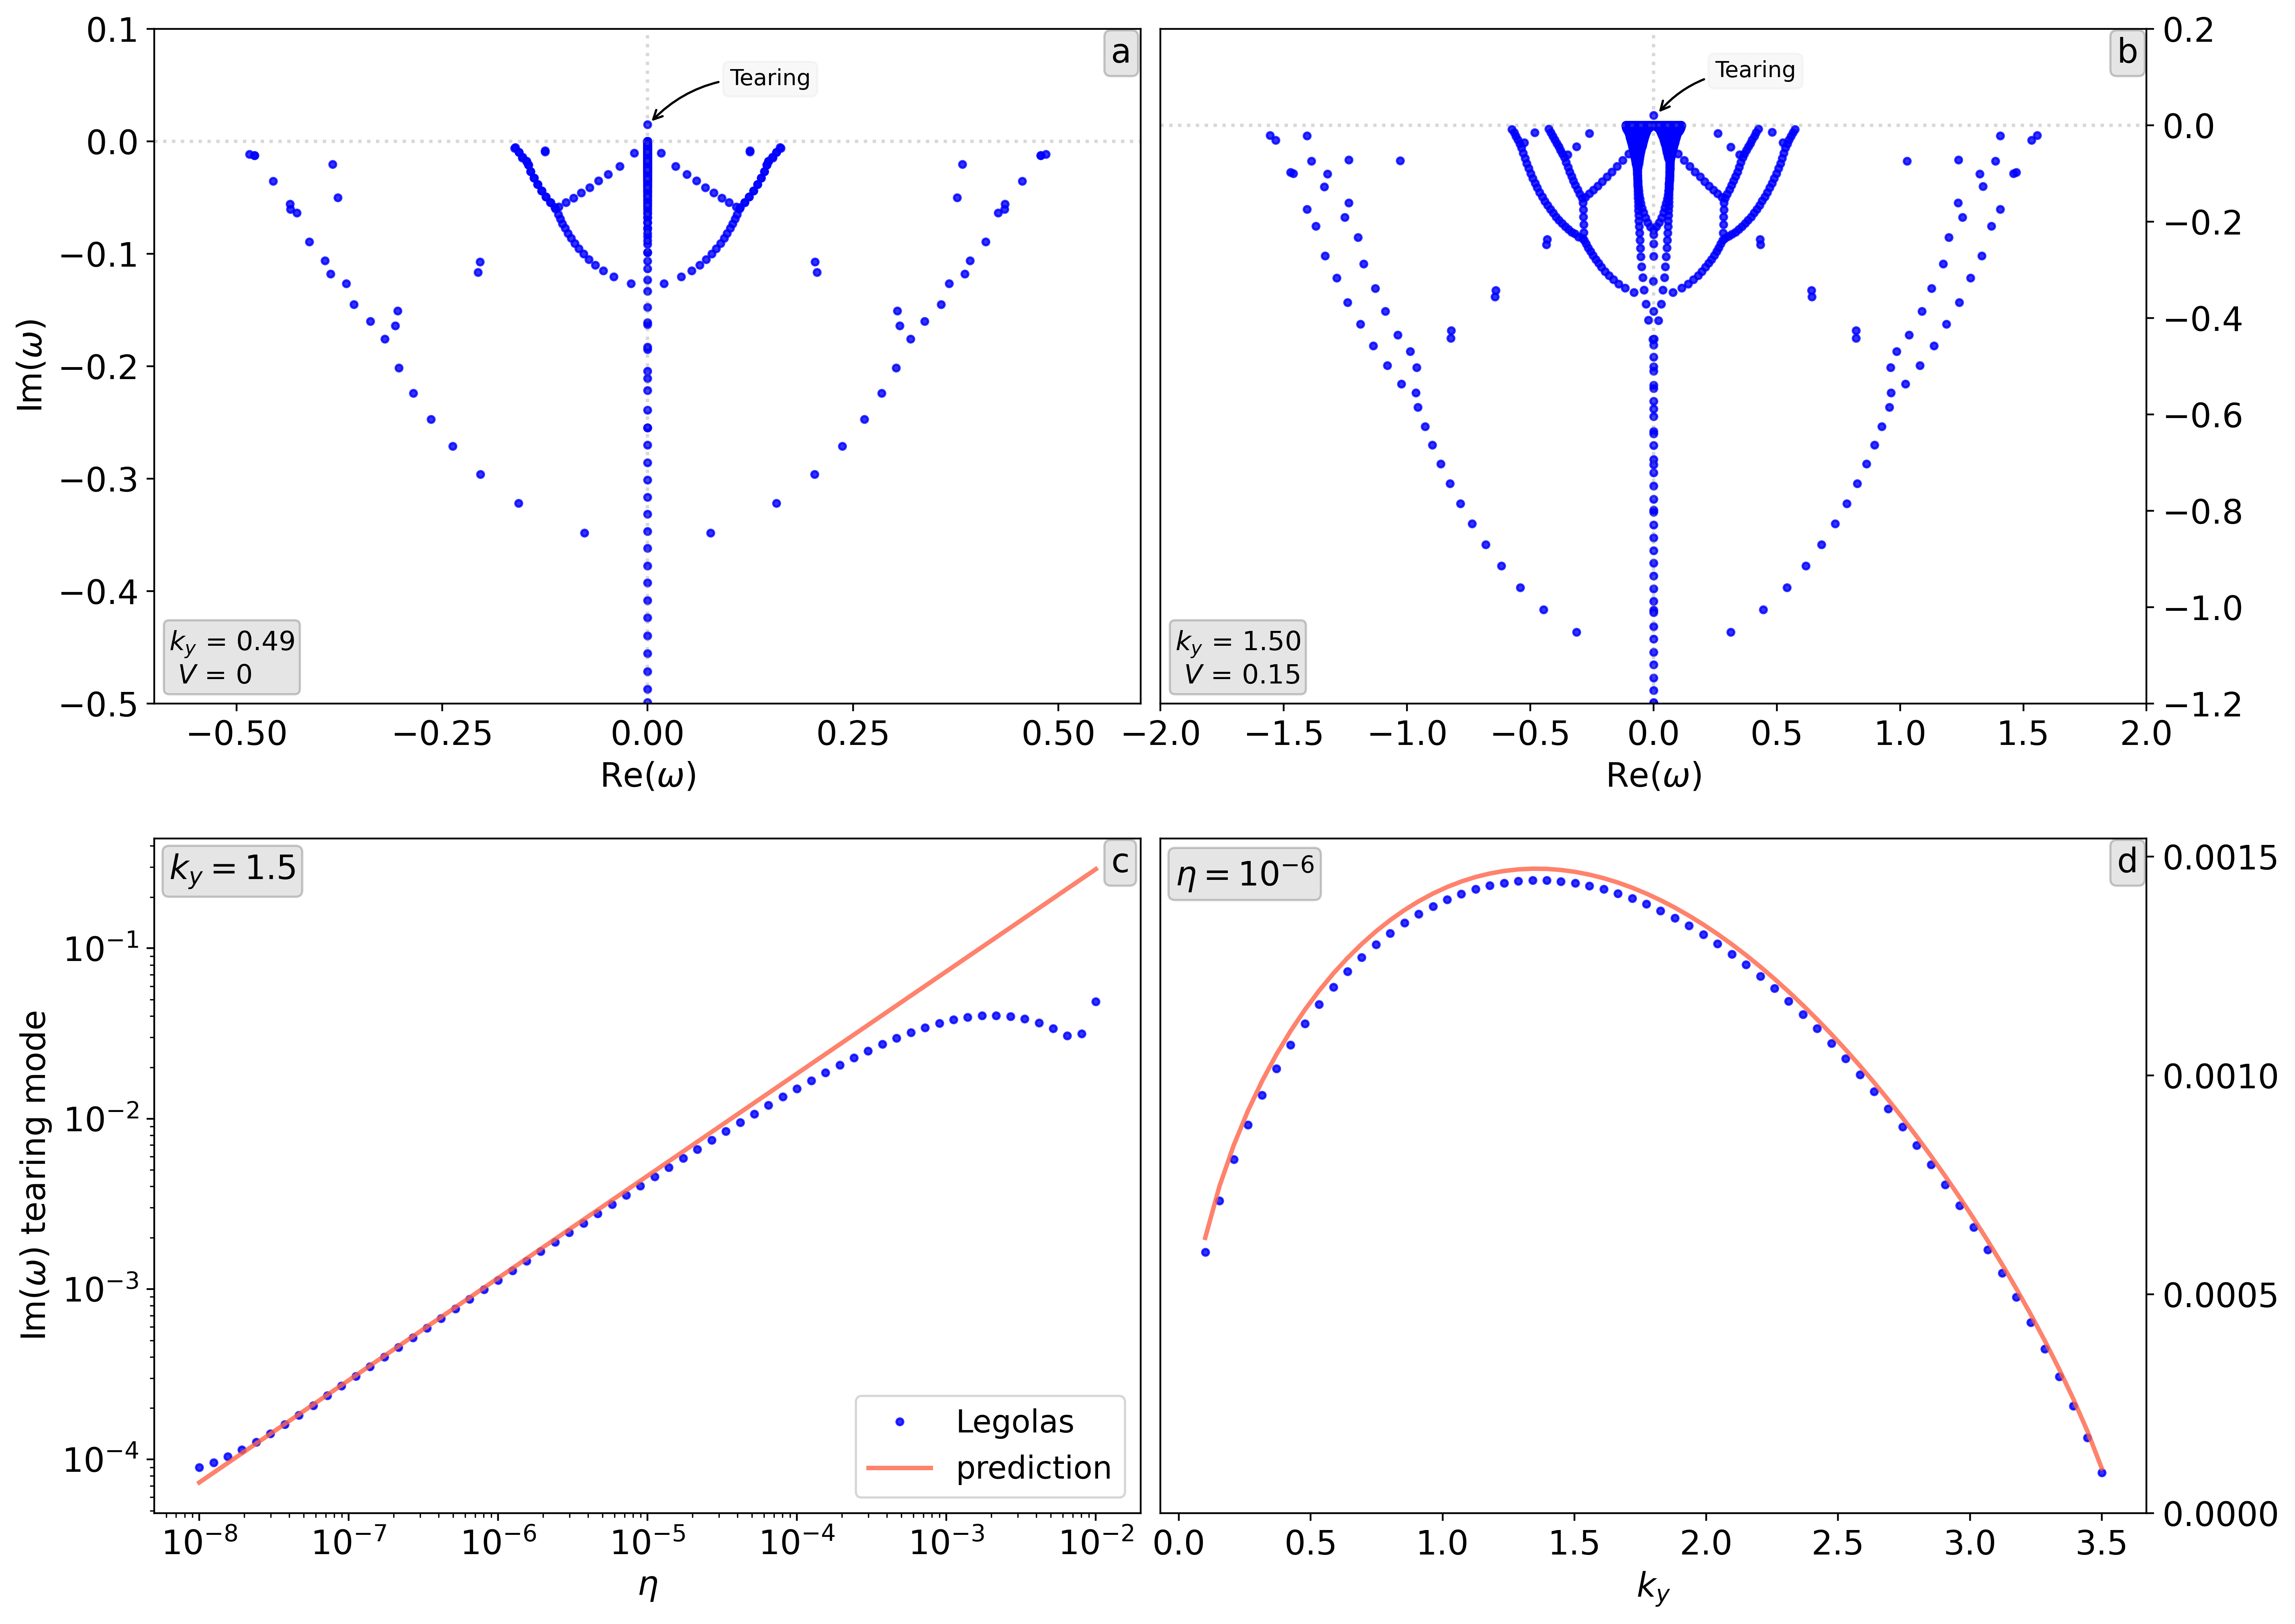
\includegraphics[width=\textwidth]{resistive_tearing.png}
  \caption{
    Resistive spectra of the equilibrium given in Equation \eqref{eq: resistive_tearing}, unstable to the tearing mode (annotated with an arrow). Panels \textbf{a} and \textbf{b} show the spectrum without and with a linear flow profile, respectively, zoomed in to reveal the complex structure of the slow and Alfv\'en modes (fast modes are not shown). Panels \textbf{c} and \textbf{d}: growth rate of the tearing mode vs. fixed $k_y$, varying $\eta$ and fixed $\eta$, varying $k_y$, respectively. Both bottom panels are cases without flow, with 64 runs of 351 gridpoints each, per panel. The red line in Panels \textbf{c} and \textbf{d} denotes the theoretical growth rate prediction given in Equation \eqref{eq: tearing_growthrate}.
  }
  \label{fig: resistive_tearing}
\end{figure}

For a thorough discussion on tearing modes, we refer to \citet{book_MHD}, where they perform a detailed analysis on the resistive MHD equations to derive an analytical expression for the growth rate of the tearing mode, given by
\begin{equation} \label{eq: tearing_growthrate}
  \begin{aligned}
    \text{Im}(\omega) &= \magneticreynolds^{-3/5}(KH)^{2/5}\left(\frac{\Delta'}{C}\right)^{4/5}\alfvenspeed / a,
    \qquad
    \text{in which} \\
    \Delta' &= -2\sqrt{H^2 - K^2}\cot\left(\frac{1}{2}\sqrt{H^2 - K^2}\right),
  \end{aligned}
\end{equation}
with $\magneticreynolds = a \alfvenspeed / \eta$ the magnetic Reynolds number, $a$ the width of the slab, and $\alfvenspeed$ the Alfv\'en velocity. The other parameters in this equation are variables introduced during the analysis, given by
\begin{equation}
  H = \alpha a,
  \qquad
  K = k_0 a,
  \qquad
  C = 2\pi\frac{\Gamma(3/4)}{\Gamma(1/2)} \approx 2.1236.
\end{equation}

Panels c and d of Figure \ref{fig: resistive_tearing} show a comparison of the tearing mode growth rate between the {\legolas} results (using the no-flow case) and Equation \eqref{eq: tearing_growthrate}. Panel c holds $k_y = 1.5$ constant but varies the resistivity, reaching Reynolds numbers of $\approx 10^8$, a feat that is nearly impossible to achieve if fully nonlinear codes would be used instead. The correspondence between the theoretical and numerical growth rates is nearly one-to-one, except for large resistivity values as the theoretical approximation starts to break down in those regimes. In Panel d we keep $\eta = 10^{-6}$ (magnetic Reynolds number of $\approx 10^6$) constant and vary $k_y$ between 0.1 and 3.5, which again yields excellent agreement between theory and numerical results. For both Panels c and d we performed 64 runs of 351 gridpoints each.



\section{Nonadiabatic, cylindrical cases}
Because {\legolas} is the first linear MHD code to simultaneously include nonadiabatic effects, resistivity, and flow, there are no known previously calculated spectra where all these physical effects are included. Nevertheless, there exist some spectra in the literature where solely nonadiabatic effects are included (and where the equilibrium is static and no resistivity is incorporated), so we will use these as a base comparison for testing the nonadiabatic terms in the implementation.

\subsection{Nonadiabatic discrete Alfv\'en waves}
The first spectrum we will look at is that of nonadiabatic discrete Alfv\'en waves, described in \citet{keppens1993}. The basic cylindrical equilibrium represents a solar loop, and nonadiabatic effects included were optically thin radiative losses and parallel thermal conduction. It was pointed out how a cluster sequence of discrete Alfv\'en waves may become unstable and could lead to disruptions or oscillatory behaviour in loops or prominences.

This particular equilibrium uses an axial current profile in a cylindrical geometry, yielding the same magnetic configuration as given in Equation \eqref{eq: tokamak_btheta} although this time with $\nu = 2$ such that a current distribution is present throughout the loop. The pressure profile can be obtained through integration of the equation for magnetostatic equilibrium \eqref{eq: force_equilibrium} without flow. As a boundary condition, we impose that the pressure vanishes at the plasma boundary $r = R$, which can be used to constrain the integration constant. Furthermore, a parabolic density profile is used, yielding an equilibrium configuration given by
\begin{equation} \label{eq: discrete_alfven_equilibrium}
  \begin{gathered}
    \rho_0 = 1 - \left(1 - d\right)\left(\frac{r}{R}\right)^2,
    \qquad
    B_{02} = \frac{1}{6}j_0 r\left(r^4 - 3r^2 + 3\right),
    \qquad
    B_{03} = 1, \\
    \begin{aligned}
      p_0 = ~&\frac{j_0^2}{720}\Bigl[
        12\left(R^{10} - r^{10}\right)
        - 75\left(R^8 - r^8\right)
        + 200\left(R^6 - r^6\right) \\ \Bigl.
        &- 270\left(R^4 - r^4\right)
        + 180\left(R^2 - r^2\right)
      \Bigr],
    \end{aligned}
  \end{gathered}
\end{equation}
in which $d = 0.2$ and $j_0 = 0.125$. The cylinder wall is taken at $R = 1$. The equilibrium temperature profile can be derived using $T_0 = p_0 / \rho_0$ and $T_0' = \left(p_0'\rho_0 - \rho_0'p_0\right)/\rho_0^2$, where the prime denotes the derivative with respect to $r$. Only conduction parallel to the magnetic field lines is taken into account,
because cross-field thermal conduction acts on too long a timescale in this case \citep{keppens1993}.

The wavenumbers $k_2 = m$ and $k_3 = k$ are taken to be 1 and 0.05, respectively. The heating term is assumed to be as such that it exactly balances out the optically thin radiative losses in the equilibrium state. We use the cooling curve introduced by \citet{rosner1978}, which represents a piecewise cooling law with predetermined coefficients. Because the inclusion of nonadiabatic effects requires us to specify unit normalisations in order to loop up the dimensional values in the cooling tables, we take reference values of 50 G for the magnetic field, $1.5 \times 10^{-15}$ g cm$^{-3}$ for the density and $10^{10}$ cm as a length scale. This automatically constrains all other normalisations through the ideal gas law, assuming a fully ionised plasma.

\begin{figure}[t]
  \centering
  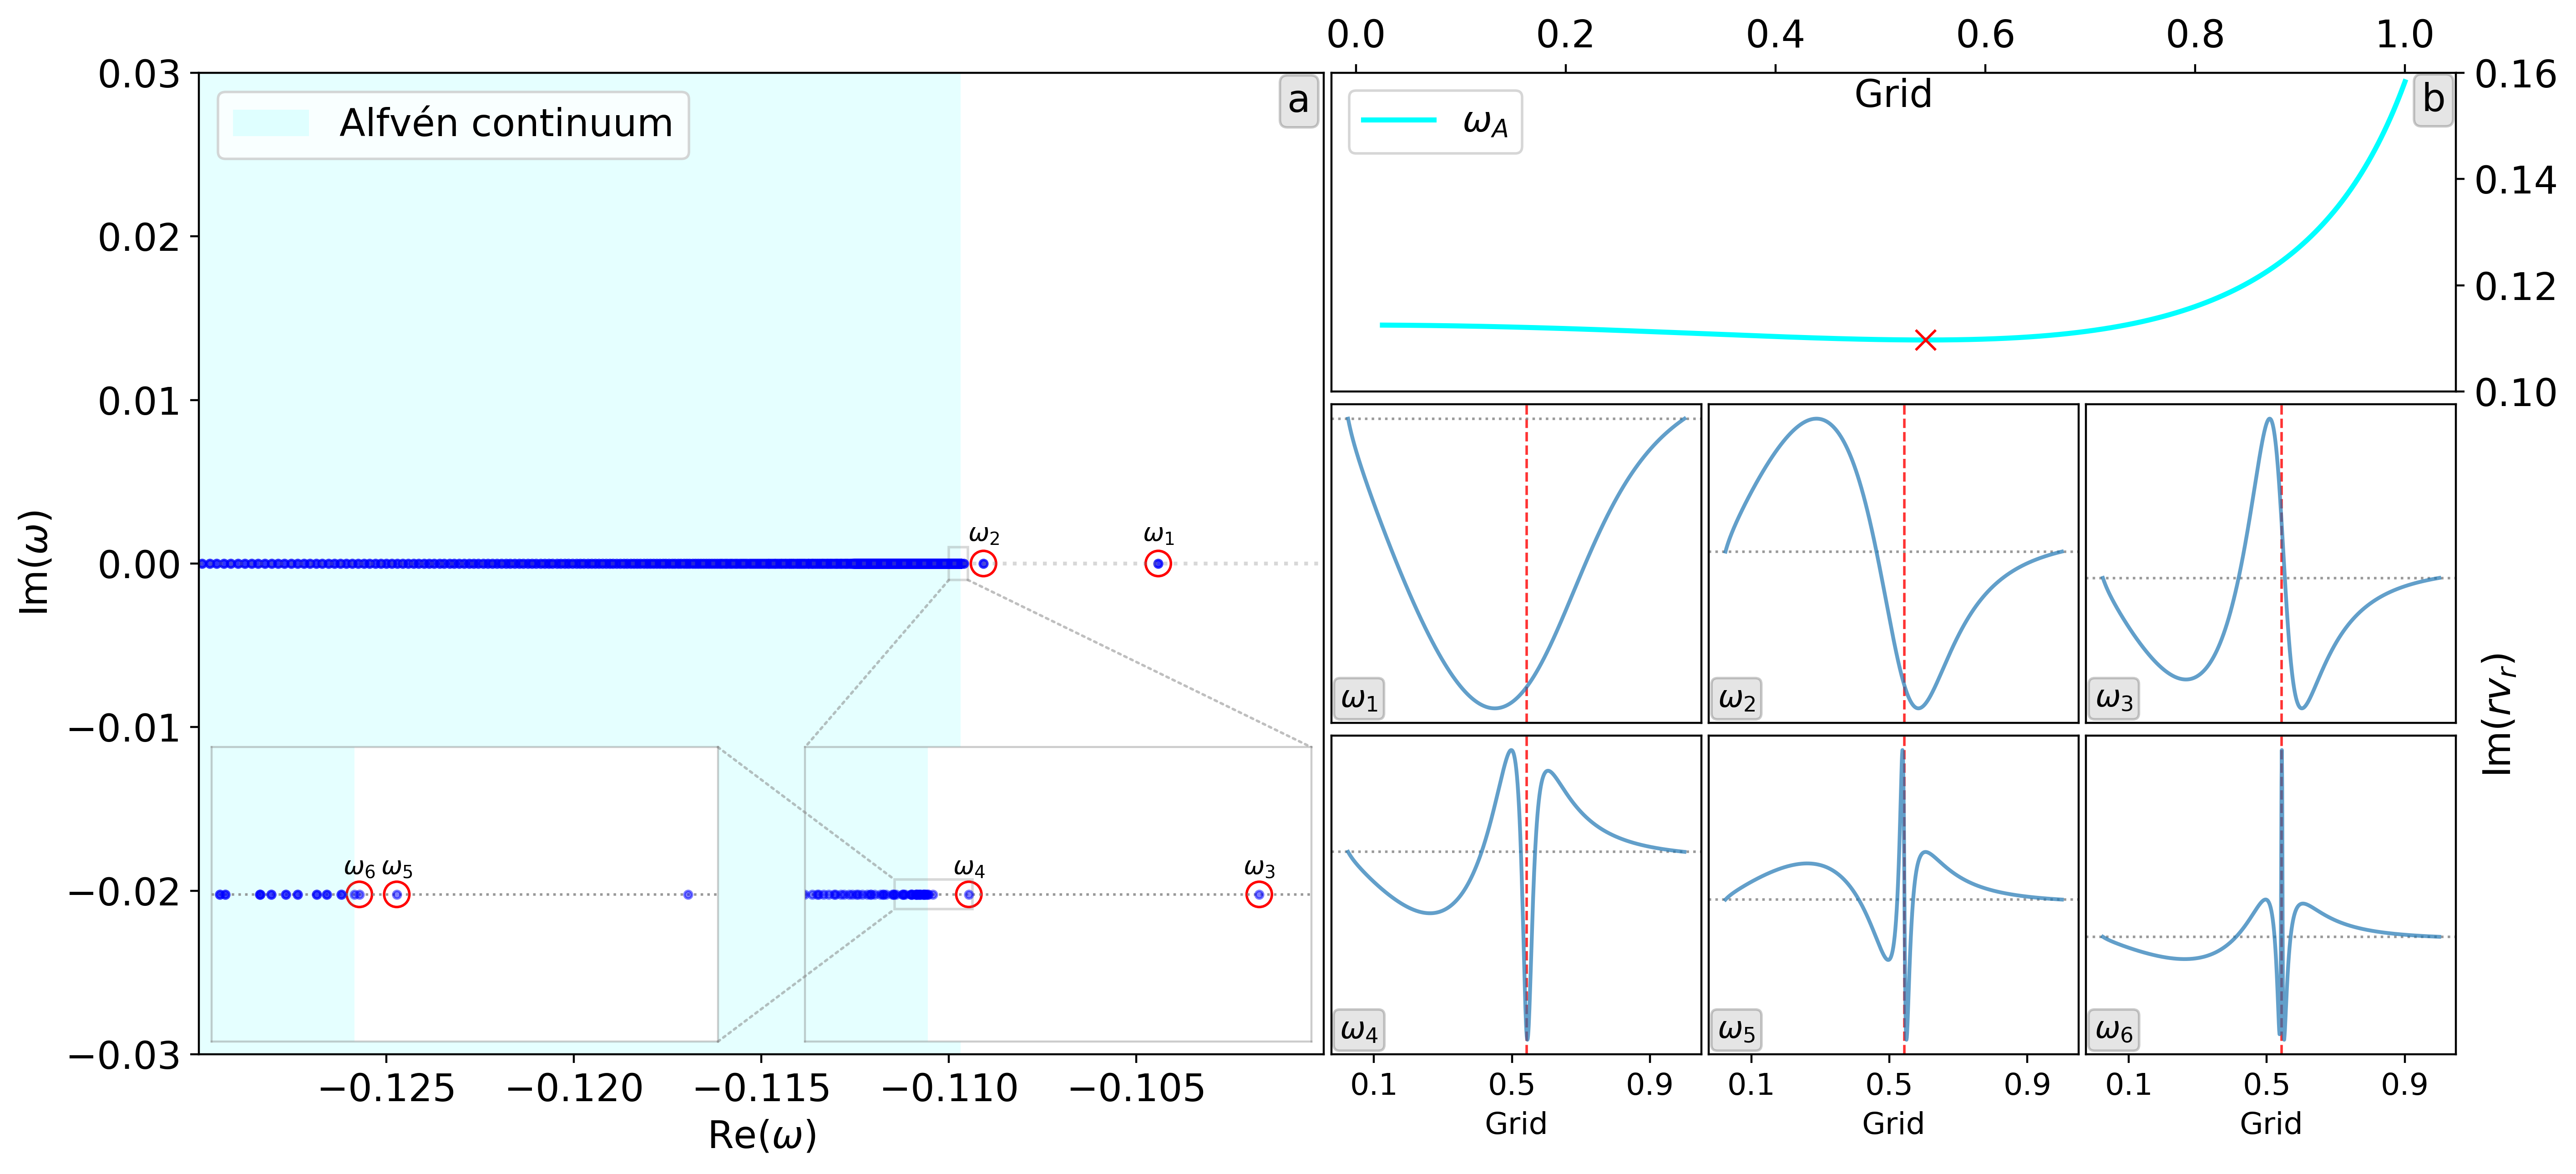
\includegraphics[width=\textwidth]{discrete_alfven.png}
  \caption{
    Panel \textbf{a}: discrete Alfv\'en spectrum; the Alfv\'en continuum is annotated in cyan. Six discrete modes were found, denoted $\omega_1$ through $\omega_6$. The insets depict zoom-ins; the regions are annotated in the figure. Panel \textbf{b} shows a plot of the Alfv\'en continuum vs. radius; the minimum is denoted by a red cross. The six panels in the bottom-right corner show the imaginary part of the $r v_r$ eigenfunctions for modes $\omega_1$ through $\omega_6$, the red dotted line represents the location of the minimum of the Alfv\'en continuum.
  }
  \label{fig: discrete_alfven}
\end{figure}

The spectrum is calculated using 501 gridpoints, Figure \ref{fig: discrete_alfven} shows the discrete Alfv\'en spectrum (Panel a) along with a plot of the Alfv\'en continuum (Panel b). In total, six discrete modes (that is, modes that fall outside of the Alfv\'en continuum) were found in contrast with the five discrete modes in the original paper by \citet{keppens1993}. The discrete modes are annotated according to their overtones, where $\omega_1$ represents the fundamental mode (FM) and $\omega_6$ the fifth overtone (OT). This last overtone does not show up for resolutions below $\sim 200$ gridpoints, which explains why it is not present in the original work. The imaginary part of the $r v_r$ eigenfunction corresponding to each of these six modes is shown in the bottom-right panels of Figure \ref{fig: discrete_alfven}, where the location of the minimum in the Alfv\'en continuum is indicated by a red dotted line. Note that the number of eigenfunction nodes increases when considering modes further in the Alfv\'en sequence: the eigenfunction corresponding to $\omega_1$ has no nodes, and $\omega_2$ through $\omega_6$ have one, two, three, four, and five nodes, respectively. Table \ref{tab: discrete_alfven} shows a detailed comparison between the discrete modes found by {\legolas} and the ones from \citet{keppens1993}.
We multiplied these latter by $\icomplex$, because they use the convention $\exp(st)$ rather than $\exp(-\icomplex \omega t)$ in the Fourier analysis (thus, $\omega = \icomplex s$).

\begin{table}[t]
	\centering
	\caption{
    Comparison of discrete Alfv\'en eigenvalues between \texttt{Legolas} and the original work by \citet{keppens1993}
  }
	\begin{tabular}{c c c}
		\hline
		\textbf{Eigenvalue}		&		\texttt{Legolas}									&				original work	\\
		\hline
      FM $\omega_1$	    &	$-0.1044166 + 1.7261\times 10^{-07}\icomplex$	&	$-0.1043688 + 1.7\times 10^{-07}\icomplex$	\\
      1st OT $\omega_2$	&	$-0.1090794 + 6.5883\times 10^{-08}\icomplex$	&	$-0.1090706 + 6.7\times 10^{-08}\icomplex$	\\
      2nd OT $\omega_3$	&	$-0.1096034 + 8.3813\times 10^{-09}\icomplex$	&	$-0.1096018 + 8.4\times 10^{-09}\icomplex$	\\
      3rd OT $\omega_4$ &	$-0.1096779 + 2.5325\times 10^{-09}\icomplex$	&	$-0.1096777 + 2.5\times 10^{-09}\icomplex$	\\
      4th OT $\omega_5$	&	$-0.1096872 + 3.7770\times 10^{-10}\icomplex$	&	$-0.1096871 + 4.0\times 10^{-10}\icomplex$	\\
      5th OT $\omega_6$	&	$-0.1096883 + 7.4336\times 10^{-11}\icomplex$	&					---
	\end{tabular}
	\label{tab: discrete_alfven}
\end{table}

In reality, the mode sequence is expected to be an infinite sequence accumulating at the local minimum in the Alfv\'en continuum, as indicated in Panel b on Figure \ref{fig: discrete_alfven}. Both the real and imaginary parts of the eigenvalues are in excellent agreement. It should be noted that when the nonadiabatic effects are omitted, the imaginary parts of these discrete modes become zero, such that they lie on the real axis, representing stable waves. The inclusion of nonadiabatic effects hence has almost no influence on their oscillation frequency and solely pushes these modes into the unstable part of the imaginary plane. In \citet{keppens1993}, it was pointed out how these discrete Alfv\'en mode sequences can be studied by means of a WKB analysis. However, this only correctly predicted the damped or overstable nature of the higher-order modes: to determine whether the most global modes of the sequence are overstable or damped requires a full numerical calculation, now possible with a tool like {\legolas}.


\subsection{Magnetothermal instabilities}
As a final test, we look at magnetothermal instabilities, originally depicted in \citet{vanderlinden1992}. The geometry is cylindrical with $r \in [0, 1]$ and an isothermal equilibrium profile given by
\begin{equation} \label{eq: magnetothermal_equilibrium}
  \begin{gathered}
    T_0 = 1,
    \qquad
    B_{02} = \frac{r}{1 + r^2},
    \qquad
    B_{03} = 0,
    \qquad
    p_0 = \frac{1}{2\left(1 + r^2\right)^2},
    \qquad
    \rho_0 = \frac{p_0}{T_0},
  \end{gathered}
\end{equation}
with $k_2 = m = 0$ and $k_3 = k = 1$. There is no $B_{0z}$, such that this configuration actually represents a z-pinch (which is very unstable), and we are looking at axisymmetric (sausage) $m = 0$ modes here. Field-aligned thermal conduction is included, cross-field thermal conduction is omitted. Optically thin radiative losses are accounted for, and we use the same cooling curve and heating assumptions as for the nonadiabatic discrete Alfv\'en waves in the previous subsection. Reference values are taken to be $2.6$ MK for the temperature, 10 G for the magnetic field and $10^8$ cm for the length scale. As before, this automatically constrains all other normalisations as well. There parameters are representative for solar coronal loops and arcades.

Both the Alfv\'en and slow continua collapse into marginal (zero) frequency. However, including finite parallel thermal conduction and radiative losses introduces the thermal continuum. Together with the marginal slow-Alfv\'en frequencies, this organises the modes such that thermal instabilities merge with magnetic modes, introducing magnetothermal branches. Figure \ref{fig: magnetothermal} shows the MHD spectrum for 1001 gridpoints in the region of the magnetothermal branches, where the bottom-right Panel c zooms in further near the origin. The modes denoted by $I_{+1}$ and $T_1$ represent fundamental magnetic and thermal modes, respectively, meaning they are not coalesced.
The overtones of these modes on the other hand are coalesced; these are denoted by $\left(I_{+2}, T_2\right)^-$ and $\left(I_{+15}, T_{15}\right)^-$ for the 1st and 14th overtones, respectively. The minus sign in superscript means they are located on the negative side of the real axis. There are corresponding modes on the positive part of the real axis, as without flow, we maintain left-right symmetry of the spectrum. The first 14 overtones are in excellent agreement with those described in \citet{vanderlinden1992} and are encircled in red on Panel a. However, the original work only displays solutions up to the 14th overtone. The resolution used here is much higher than the originally published results, allowing us to probe the region near the origin as well. Panel c zooms in near the origin, denoted by the dashed rectangle in Panel a, revealing a complex mixture of different branches and scattered modes. It seems that the original magnetothermal branches split, and a dense region covered with many magnetothermal modes appears. The (analytically known) thermal continuum is annotated in green on the figure, and is represented by a dense, continuous range of discrete eigenvalues on the imaginary axis. Because this is the first time that such high resolutions are possible for computing the magnetothermal modes, it is left to future work to clarify how the MHD spectrum allows for such complex mode interactions, revealing the possible presence of areas covered by modes in the complex eigenfrequency plane.

\begin{figure}[t]
  \centering
  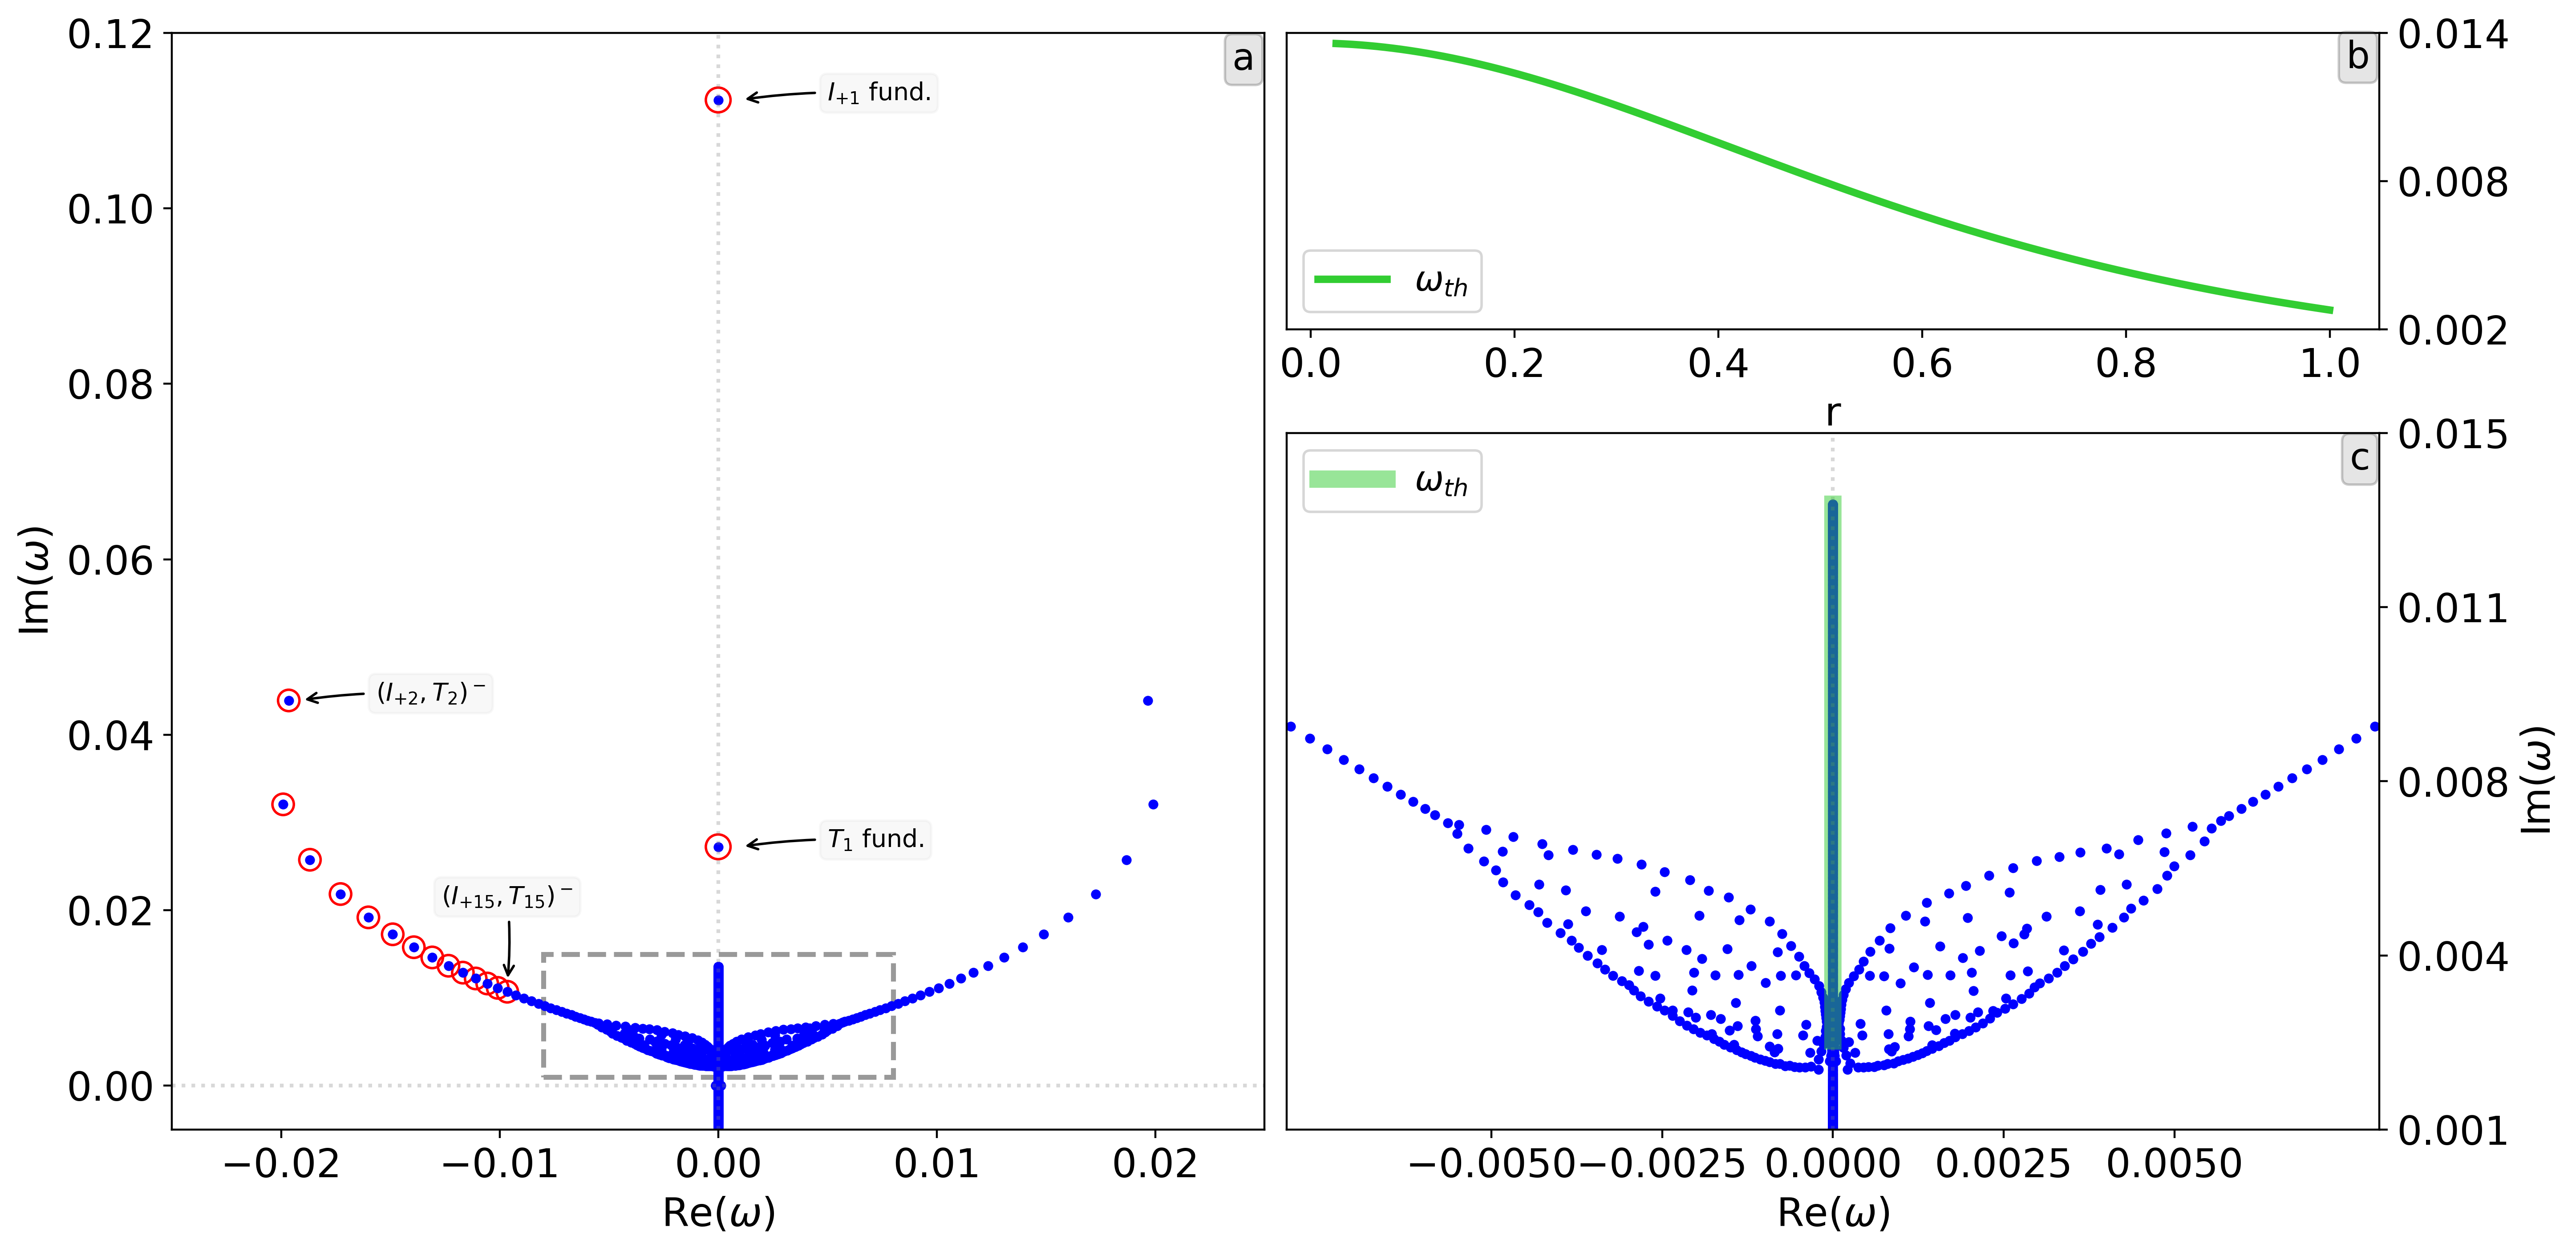
\includegraphics[width=\textwidth]{magnetothermal.png}
  \caption{
    Magnetothermal instabilities for $m = 0$ and $k = 1$. The fundamental modes and 14 overtones discussed in the original work are encircled by red and denoted in the left Panel \textbf{a}. Panel \textbf{b} shows the thermal continuum as a function of radius. Panel \textbf{c} zooms into the region denoted by dashed lines in Panel \textbf{a}, revealing various other modes forming intricate structures.
  }
  \label{fig: magnetothermal}
\end{figure}

\section{Convergence} \label{sec: convergence}
As is clear from all cases discussed in this Chapter, increasing the resolution can have a major influence on the spectrum, depending on whether or not all modes are sufficiently resolved. Generally speaking, the further one goes in a specific sequence, that is, looking at larger mode numbers that represent overtones having more and more nodes in their eigenfunctions, the higher the resolution that is required in order to resolve the mode completely. For eigenfunctions, it is usually immediately clear if a mode is resolved or not, because higher mode numbers translate into more oscillations in the eigenfunction. Hence, once the number of oscillations approaches the amount of gridpoints, the eigenfunction will no longer be resolved.

For the eigenfrequencies it is not a priori clear when a specific $\omega$ is resolved. One way to constrain an eigenvalue is to do multiple runs, each time increasing the resolution. Once an eigenvalue no longer shifts in the complex plane, it can be considered resolved, and increasing the resolution even further will not have much effect on its value. Now, the question of how many gridpoints are typically needed to be able to speak of a ``resolved'' spectrum naturally arises. This will strongly depend on the type of equilibrium considered: for smooth equilibria without sharp transitions, one can get away with a few dozen gridpoints and already reach an acceptable accuracy for most modes. However, in the case of equilibria with large gradients, or even with localised discontinuities (interfaces), one has to make sure that a sufficient number of gridpoints are taken in order to sufficiently resolve that jump.

Furthermore, the amount of eigenvalues in the spectrum increases with resolution, because there are as many eigenfrequencies as the dimension of the matrices (which is 16 times the number of gridpoints, at least for the 8 MHD equations). It is therefore entirely possible that one starts probing parts of the spectrum that were initially not visible at lower resolutions, simply because there were no eigenvalues in that region for that amount of gridpoints. An example is given here, where we look back at the Kelvin-Helmholtz equilibrium discussed in Section \ref{ss: kh_cd_instabilities}. Figure \ref{fig: convergence} shows this equilibrium for the exact same values as employed earlier, but every panel shows the spectrum for a different resolution, with the amount of gridpoints given in the top-left corner. The first three panels start out at low resolution, increasing from 26 to 76 gridpoints. Three modes are annotated on the figure, corresponding to the KH and CD modes discussed earlier. These modes are already decently resolved even at the lowest resolutions and can be considered completely resolved at around 100 gridpoints. However, the region near the horizontal axis is another matter entirely. At low resolutions (first three panels), we see that most of the modes here are almost randomly scattered in the complex plane. At around 100 gridpoints, they start lining up and form a more intricate ``elliptic'' pattern. This is the point where the original paper by \citet{baty2002} stopped, because back then it was not really feasible to run these codes at higher resolutions, and they were only interested in the most unstable KH and CD modes that were resolved, and that determined the early evolution of a full nonlinear MHD simulation that they performed.

\begin{figure}[t]
  \centering
  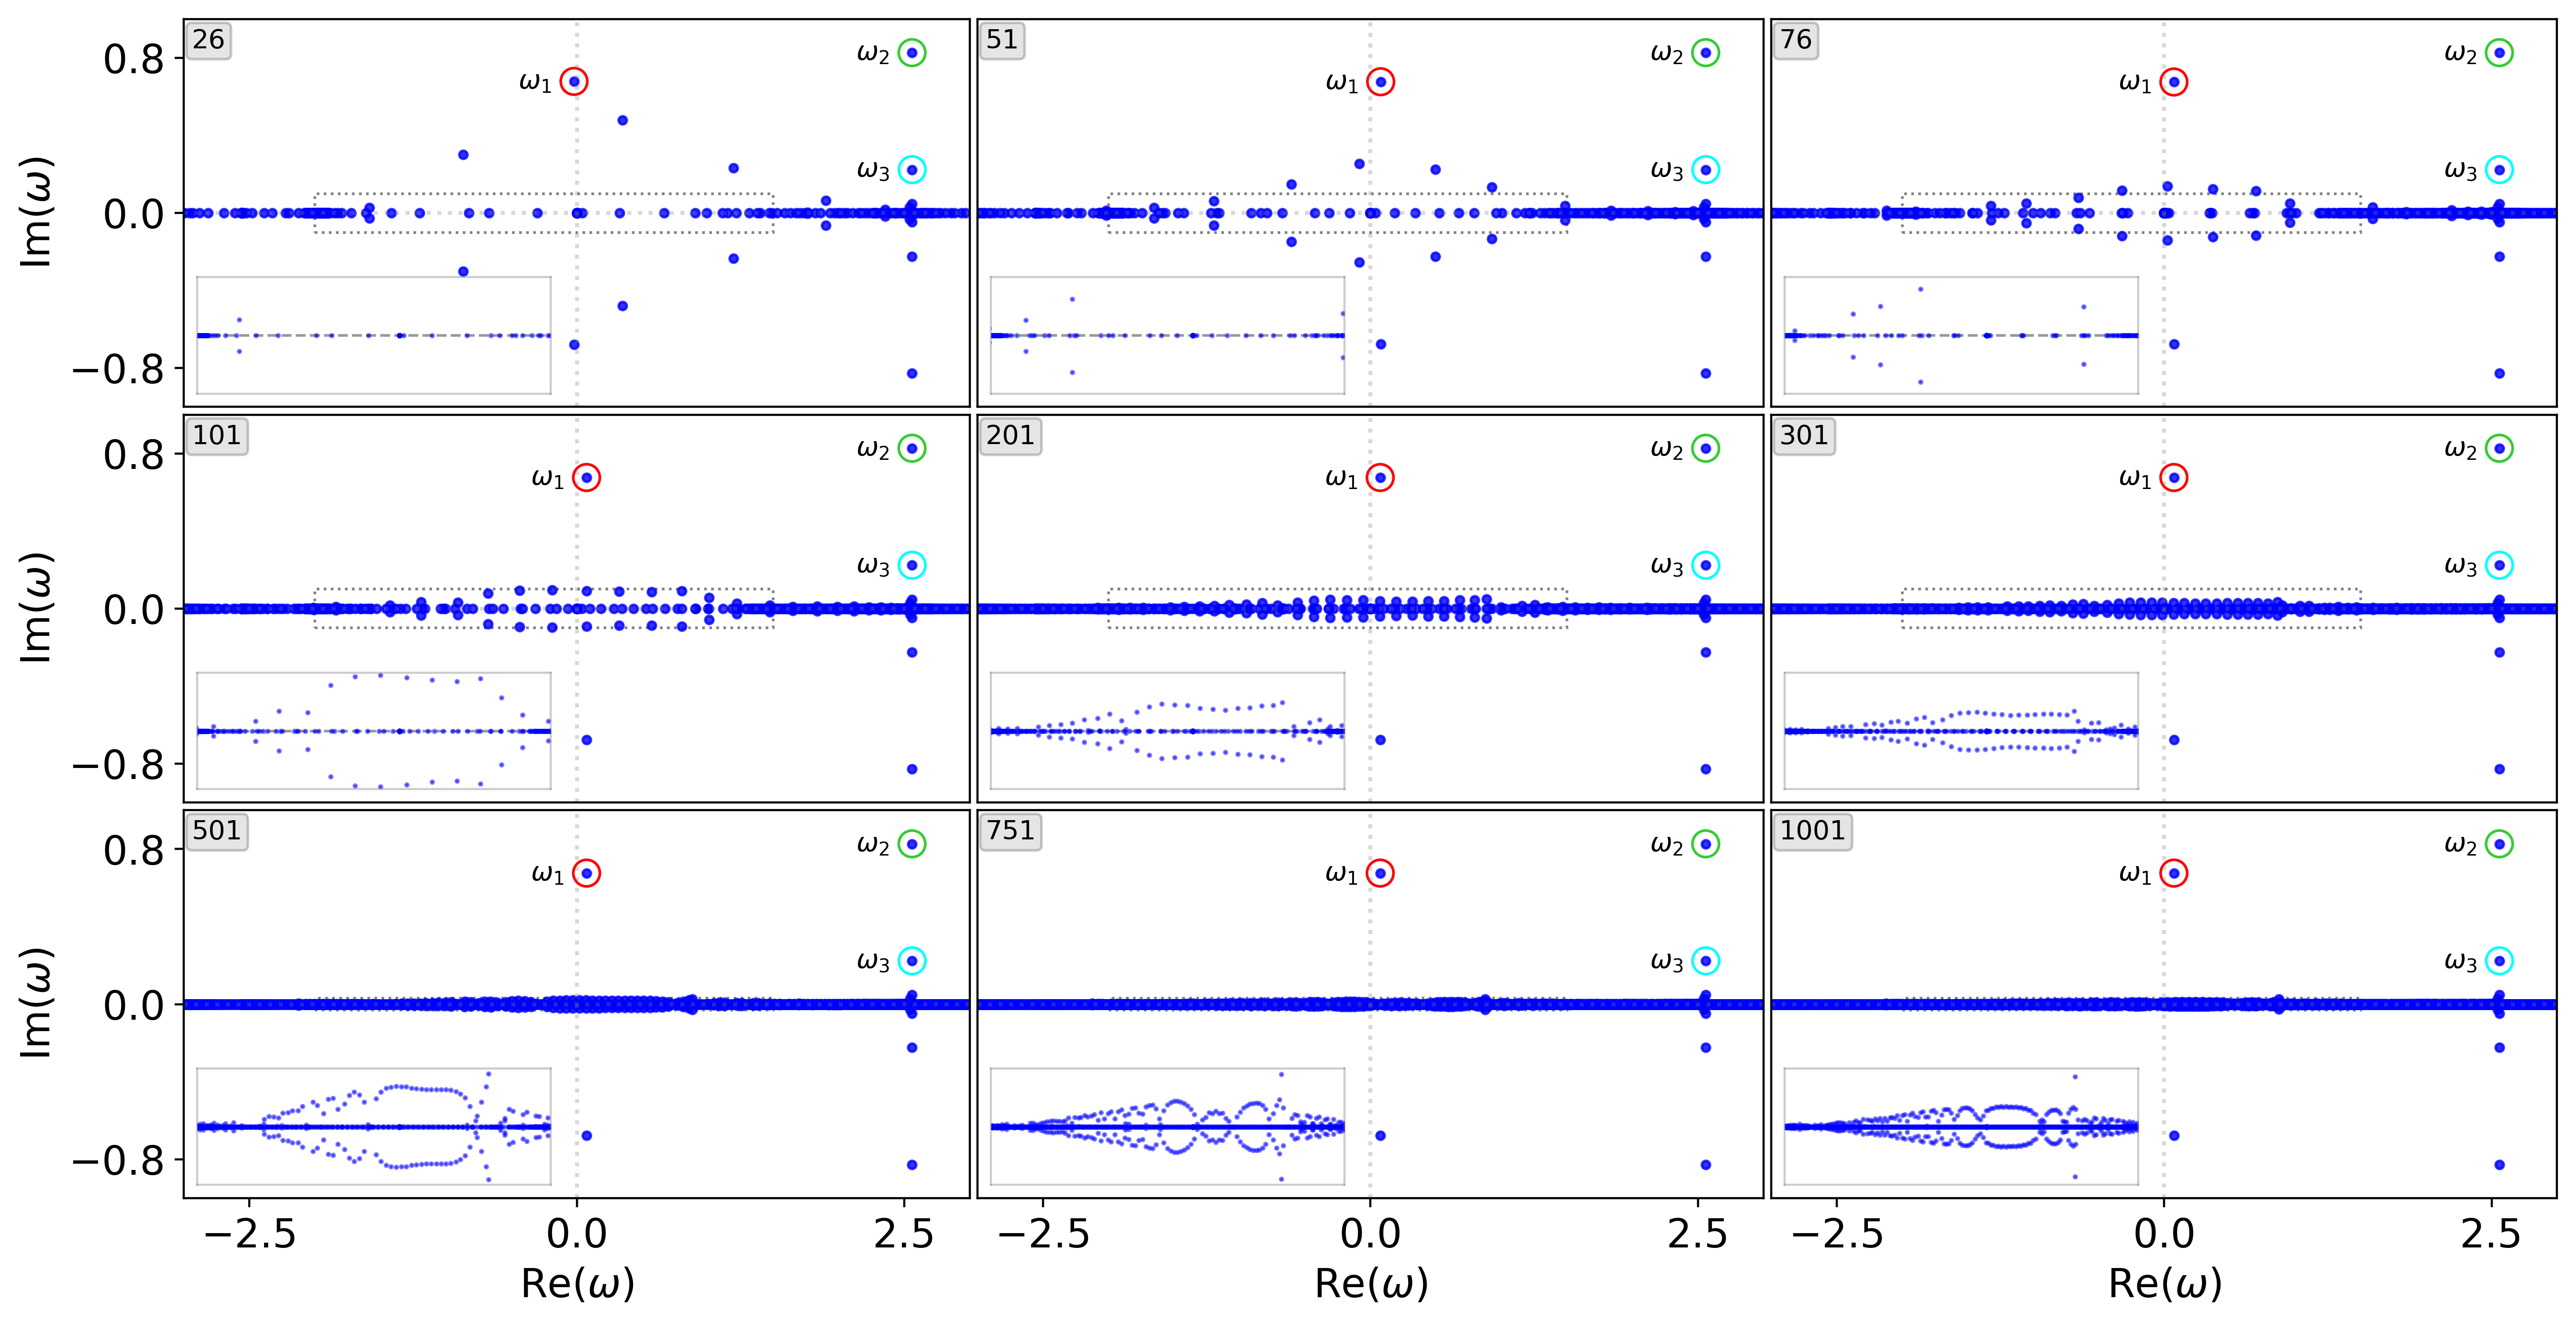
\includegraphics[width=\textwidth]{convergence.png}
  \caption{
    Spectrum of the Kelvin-Helmholtz and current-driven equilibrium as shown in Figure \ref{fig: kh_cd}, using the same parameters as in Section \ref{ss: kh_cd_instabilities}, at various resolutions (indicated on the top-left of each panel). The inset on the top two rows of panels zooms near the horizontal axis, for vertical axis values between $-0.1$ and $0.1$. The insets on the bottom row of panels have slightly different vertical bounds, from $-0.03$ to $0.03$.
  }
  \label{fig: convergence}
\end{figure}

When the resolution is increased even further, we see that the near-axis modes shift even closer to the real eigenfrequency axis, and as visible on the insets of each panel, these modes start to form intriguing patterns at high resolutions. The amount of ``scattered'' modes decreases considerably, and a helix-like structure is formed at very high resolutions (1001 gridpoints, lower-right panel). These complex and almost geometric patterns may arise in various different equilibria as well and call for extensive research in this topic. A complementary means to identify which modes are actually resolved is to exploit the spectral web; see \citet{goedbloed2018_web1, goedbloed2018_web2} and \citet[Ch. 12--13]{book_MHD}, who locate eigenmodes on specific curves and their intersections. These curves relate to the two self-adjoint operators at play in stationary, adiabatic MHD. Only a combined approach using high-resolution {\legolas} runs, modern linear algebra solvers, and physical insight in MHD spectral theory will in time reveal the true importance of these modes.

Based on the conclusions drawn here, it is clear that the resolution required depends on the part of the spectrum that is to be investigated. For isolated modes, about 100 gridpoints is usually more than sufficient to resolve most of them, although this also depends on the equilibrium under consideration. For large-scale surveys of the spectrum, large resolutions should be employed in order to reveal possible regions of interest.


\section{The Legolas testing framework} \label{ss: legolas_testing}
As with any newly developed numerical code, a proper and extensive testing framework is (supposed to be) an integral part of the development process. Every step of the way a developer should make sure that newly added code actually works and does what it is supposed to do; at the same time proper care must be taken to make sure that previously working code does not get broken due to newly added changes or features. For small codebases this can be done through a quick manual check, but this rapidly becomes cumbersome and even impossible for larger projects. {\legolas} falls in this second category, where it becomes unfeasible to manually check every single equilibrium against known results for every change made to the code. Ideally then, this process should happen automatically, which is where the testing framework comes in. Before simply writing ``tests'' however, one should carefully think about \emph{what} should be tested and \emph{how} tests are written. A test should be robust, meaning that it should be easily ported over to other platforms; and at the same time be as sensitive as possible to any breaking changes, meaning tests should fail as soon as inconsistencies are introduced. Additionally, tests should be able to run in a reasonably small amount of time. Care should also be taken to make the tests as independent of the code itself as possible: a scenario where the tests themselves have to be continuously modified following minor changes in the code base should be avoided at all cost.

The {\legolas} testing framework is split up in three main parts: \emph{unit tests}, which test individual code subroutines completely independently of one another; \emph{regression tests}, which test spectra and eigenfunctions against known results; and \emph{Pylbo tests}, which test the data reading routines and post-processing logic. These latter tests are linked to the post-processing framework \textsf{Pylbo}, which was developed along with {\legolas}, but we will not go into detail on those here.

\subsubsection{Unit tests}
The backbone of the testing framework is the unit tests, which are specifically designed to ensure that a particular part of the code (a ``unit'') works as intended. Usually one or more unit tests target a single subroutine, call it with a particular set of parameters that are chosen in such a way that the expected result is known, and the subroutine's output is compared against this known result. In most cases one subroutine is accompanied by multiple tests, where every single test handles one specific case. This also includes ``edge cases'', that is, sets of parameters that may trigger some special behaviour in a subroutine. For example, consider a subroutine with as sole purpose to find a specific value in an array and return its index. This may have a couple of tests: one or two are checking that returned values are actually the ones that we expect; at least one test is checking that the routine fails to return anything if the value is not found in the array; and at least one test checks that edge cases are properly handled, such as multiple elements with the same value in the array or accessing the array out-of-bounds.

The main advantage of unit tests is that they are independent of other routines, hence bugs that are introduced can be quickly narrowed down based on the failing units -- provided these properly cover all parts of the source code. Confidence in newly developed routines will increase considerably if tests pass, and potential bugs can be caught early on. {\legolas} makes use of the open-source pFUnit framework, originally created by developers from NASA and specifically designed for unit testing of (MPI-parallel) software written in Fortran. Figure \ref{fig: unit_test} shows an example of a unit test, where the \textsf{{@}test} decorator above the subroutine marks this as a test. In this particular case an elemental function \textsf{is\_NaN} is tested, which checks a given double-precision value or array for NaN (Not a Number) values. The \textsf{{@}assertFalse} and \textsf{{@}assertTrue} statements in turn check that the function returns what is expected, and the test will fail if one or more conditions are not true when they should be, or vice-versa.

\begin{figure}[t]
  \centering
  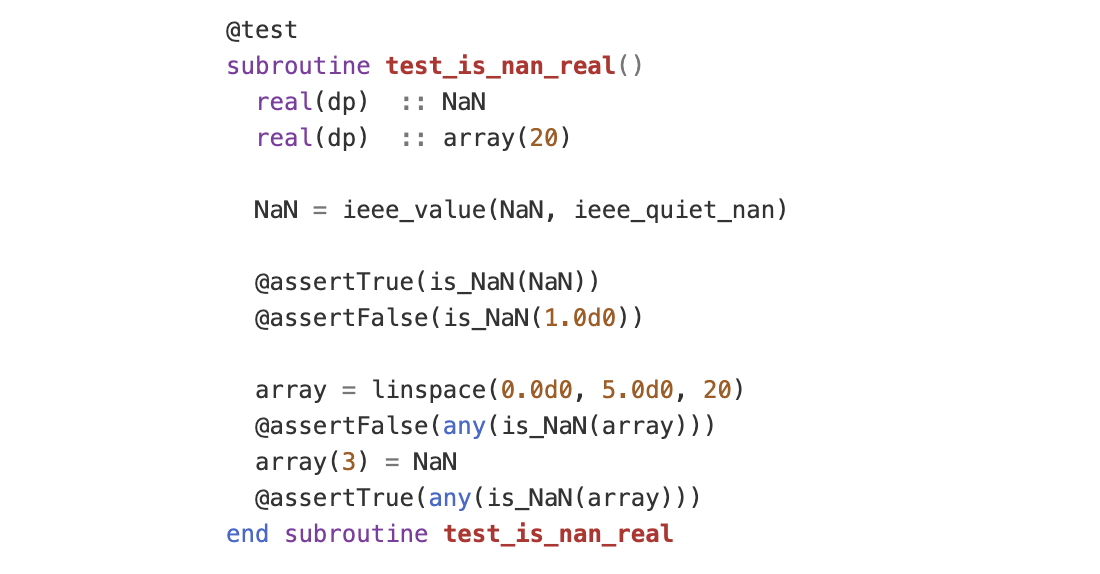
\includegraphics[width=0.80\textwidth]{unit_testing.png}
  \caption{
    Example of a {\legolas} unit test, using the pFUnit framework.
  }
  \label{fig: unit_test}
\end{figure}

\subsubsection{Regression tests}
The most important part of the testing framework are the regression tests. While unit tests are a necessary requirement to check individual subroutines and functions, they do not guarantee that the solutions to the eigenvalue problem are still the same after a code change. Additionally, it is quite difficult for the unit tests to cover everything; the matrix elements for example are quite difficult to test individually, and for those we have to resort to other approaches. The idea behind the regression tests is quite straightforward: compare the solutions, that is, both the eigenvalues and eigenfunctions, to previously (known) solutions for the implemented equilibria. However, there are a few caveats that must be addressed first: the main problem here is that we want to compare \emph{numerically calculated eigenvalues} on large scales, meaning that the actual testing is not as simple as ``just comparing solutions''. Suppose we have calculated eigenvalues for a certain equilibrium, and we know that these are correct based on a comparison with theoretically derived solutions. We call these results the ``base'' answers and store them in an array $S_\text{base}$. After a while the tests are being rerun after a change in the code base, and the solutions to the exact same problem are calculated again using the ``new'' code. Say these results are stored in an array $S_\text{test}$, resulting in the following six solutions

\begin{equation}
  \begin{aligned}
    S_\text{base} &=
      &&1.5
      &&-2 + 3\icomplex
      &&\quad 0
      &&\qquad\quad 2\icomplex
      &&-0.5\icomplex
      &&-1 - 1.0\text{e}^{-8}\icomplex \\
    S_\text{test} &=
      &&1.5
      &&-2 + 3\icomplex
      &&1\text{e}^{-15}
      &&-1\text{e}^{-16} + 2\icomplex
      &&-0.5\icomplex
      &&-1 - 1.1\text{e}^{-8}\icomplex
  \end{aligned}
\end{equation}

Note that these tests may run on different machines running different operating systems; additionally different compilers or library versions (such as for BLAS and LAPACK) may be used, which in turn can give slightly varying solutions. One can naively start comparing these two arrays, but will quickly run into a couple of problems. First of all, there is no strict guarantee that the \emph{ordering} of the solutions is the same, meaning the array needs to be sorted first. If we decide to sort based on the real part first, followed by the complex part, then the test for the above two arrays will immediately fail. While the third and fourth item of $S_\text{base}$ are saved as 0 and $2\icomplex$, the third and fourth item of $S_\text{test}$ have \emph{numerically zero} parts, with a very small but finite (up to machine precision) value deviating from zero. When $S_\text{base}$ gets sorted, 0 will be placed before $2\icomplex$, while for $S_\text{test}$ the $1\text{e}^{-15}$ solution will be sorted \emph{after} $-1\text{e}^{-16} + 2\icomplex$; resulting in the wrong eigenvalues being compared with one another.

One could argue here that a solution would be to force small values deviating from zero to actually be zero. This immediately gives rise to another problem: what is ``small''? Note that we are not comparing fixed arrays with machine precision variations, we are comparing numerical solutions to an eigenvalue problem where machine precision variations may give rise to solutions that actually differ more than machine precision. Furthermore the tolerance is eigenvalue-dependent: imagine a difference between base and test results of $10^{-6}$; for an eigenvalue of 2.5 this is perfectly fine, and the test should pass. However, for an eigenvalue of $3 \times 10^{-6}$ this is clearly too much, and the test should fail. These situations are fairly common, as the complexity of MHD spectra may result in solutions that differ many orders of magnitude within a single spectrum.

We could try opting for a percentage-based comparison, or absolute versus relative differences, but then again, \emph{how do we specify the tolerance}? As we just mentioned this is problem-specific, and we do not want our tolerances to be too robust since then we might miss out on important changes in the spectrum. No matter the solution employed here -- be it checking for absolute values, relative differences, separate real/imaginary parts, etc. -- we will eventually always run into a special case in which our strategy will fail due to numerical variations in calculating the eigenvalues.

Clearly, directly comparing eigenvalues to each other is not the right approach. A much better strategy is to compare the \emph{locations} in the spectral plane, where we actually plot the spectrum and highlight position shifts in the eigenvalues. This will eliminate much of our numerical issues, and we can ensure that the way the spectrum is drawn happens in exactly the same manner across different platforms. In {\legolas}, the regression tests are handled as follows
\begin{enumerate}
  \item[i)] For a given test, load the file with stored results and plot (at least one) spectrum with given limits for the real and imaginary axes, save the image(s) as baseline.
  \item[ii)] Execute the corresponding test, plot the spectrum for the obtained results with the exact same settings used to create the baseline figure. Save the image(s).
  \item[iii)] Load both the test and baseline images, remove everything (background, axes, axes ticks etc.) except the eigenvalues. Calculate the Root-Mean-Squared (RMS) pixel difference between the two images as
  \begin{equation}
    \text{RMS} = \sqrt{\text{mean}\Bigl(\left(\text{expected} - \text{actual}\right)^2\Bigr)}.
  \end{equation}
  \item[iv)] Set a strict RMS tolerance, check whether the calculated RMS lies within this tolerance. If this is not the case fail the test, otherwise flag it as a pass.
\end{enumerate}
The above testing strategy has proven to be very successful, both in terms of robustness and reliability. An example is given in Figure \ref{fig: regression_test}, where the Suydam cluster spectrum from Equation \eqref{eq: suydam_equilibrium} is shown both as a baseline and for a small shift in parameters. At first sight both spectra are similar, however the RMS shows clear difference between the spectra, failing the test. The main advantage of this approach is that we can generate as much image comparisons as required: for one equilibrium we typically calculate the solutions to the eigenvalue problem once, and then generate baseline images for different parts of the spectrum. This allows for spectrum testing at different scales, where we can zoom in and focus on different regions for more accurate testing.

\begin{figure}[t]
  \centering
  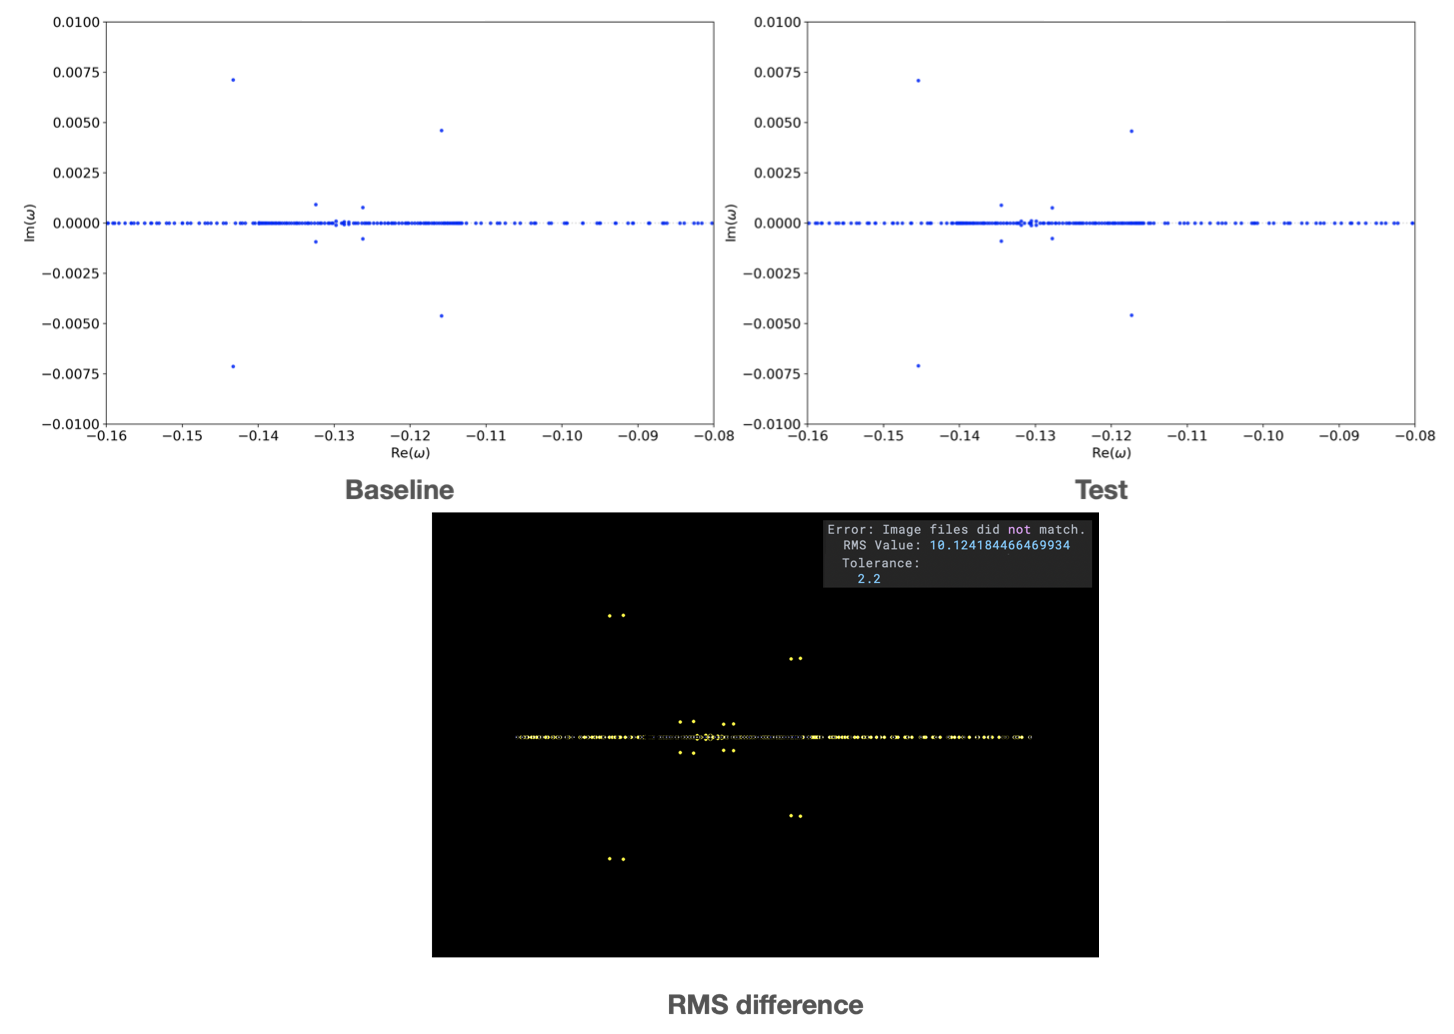
\includegraphics[width=\textwidth]{regression_testing.png}
  \caption{
    A typical example of a {\legolas} regression test, here for the Suydam cluster equilibrium. The top two images indicate the baseline spectrum (stored answer) and test spectrum (calculated answer), respectively. The bottom image shows the Root-Mean-Squared pixel difference between the top two images, the calculated RMS ($\approx 10$) is much larger than the tolerance RMS ($= 2.2$).
  }
  \label{fig: regression_test}
\end{figure}

\section{Discussion} \label{ss: legolas_discussion}
In the previous Chapter we introduced the novel finite element code {\legolas}, meant to tackle the complete MHD spectrum including all kinds of physical effects, and able to look at various realistic equilibrium configurations. The general formalism introduced can handle both Cartesian and cylindrical geometries, and with the various physics included in the formalism this makes {\legolas} the first MHD spectral code to combine the effects of flow, resistivity, gravity, radiative cooling, and anisotropic thermal conduction, even supplemented with selfgravity, viscosity or Hall MHD. This opens the door to novel, in-depth studies of the complete MHD spectrum, which was up to now impossible with existing numerical tools.

In this Chapter we tested {\legolas} against various previously established results from the literature, looking at the comparison to analytical results as well as to spectra previously obtained by similar numerical codes. Correspondence with existing results is in most cases one to one, greatly increasing the confidence in the new tool. Some cases were run in (much) higher resolutions than their original counterparts, revealing interesting features and additional structure in the spectra. As can be seen when looking at the instabilities of a cylindrical magnetised jet flow in Section \ref{ss: kh_cd_instabilities}, the outer KH and CD modes are in perfect correspondence with the original results. However, the high resolution revealed complex structures that were not probed before, and this becomes even clearer in the convergence study of Section \ref{sec: convergence}, where we used the same setup but increased the resolution even further. It is clear the the spectrum evolves drastically at higher resolutions, when more and more modes are becoming properly resolved. Because a complete knowledge of the MHD spectrum of flowing equilibria is lacking, tools like {\legolas} and careful converged studies will be essential to unravel the role as of yet unresolved spectral structure.

We speculate that these spectral structures have a physical meaning, which can be corroborated in adiabatic flowing cases with a complementary spectral web approach. Our speculation extends to cases that address MHD modes in cylindrical accretion disks \citep{keppens2002}, where it is becoming clear that many more modes than the celebrated MRI enrich the spectral structure. This has been confirmed in recent work by \citet{goedbloed2022_sari} where the SARI modes were found to be of essential importance in instability studies of accretion disks around black holes. These modes appear to open up completely new pathways to turbulence, highlighting the importance of a linear eigenmode perspective for dynamical systems even further.

Also in nonadiabatic cases interesting things were encountered: the outer modes of the magnetothermal sequence are again in perfect correspondence with modes found in the original work; however, near the origin -- a region that has never been investigated until now -- there are indications of a splitting of the magnetothermal sequence in its thermal and magnetic counterparts with various modes scattered in between. An in-depth study of magnetothermal instabilities is called for, a topic of research that essentially stopped progressing for the last two decades. Now that high-resolution MHD simulations start to reveal the complexity of thermal-instability-driven evolutions, a revival of this topic is urgently needed.

As a side node it can be argued that a standard Fourier decomposition as done in all cases discussed in this Chapter (and the previous one) misses out on non-modal growth, that is, so-called transient modes, which have been shown to be of significant importance in resistive systems \citep{mactaggart2018}. However, a calculation of the complete spectrum may very well be all that is needed; transient growth may well be a consequence of solving an actual initial value problem using a Laplace transformation, while taking all discrete and continuous modes into account. A detailed proof is far from evident, however, in adiabatic cases we have self-adjoint operators (one for a static case, two if flow is included), such that it seems plausible that a full decomposition in terms of a complete basis of eigenfunctions is possible. The inclusion of flow makes these eigenfunctions non-orthogonal, while in ideal, static plasmas the eigenfunctions are orthogonal \citep[Chapter 12]{book_MHD}. For non-ideal, stationary plasmas non-orthogonality can again be expected. How this decomposition would be affected by the inclusion of non-adiabatic effects such as resistivity, viscosity, or conduction/cooling, is not a priori clear. The possible role of transient growth in the context of thermal modes certainly warrants further investigations, and may provide a complementary picture in linear stability analysis. The discussion of transient growth is usually done in the context of non-modal analysis and uses the concept of pseudo-spectra, that is, also allowing for modes that are nearly eigenvalues.

All of the above is clear indication that a thorough investigation of the entire spectrum is needed in order to yield new insights in (M)HD instabilities. For solar applications alone, the effect of thermal conduction on the modes as indicated by \citet{vanderlinden1991} has never investigated in fully realistic setups, possibly allowing for a deeper understanding of fine structure in solar prominences. Since {\legolas} is such a versatile code the possibilities are endless: from various hydrodynamic configurations to more magnetically oriented astronomical cases like accretion disks or astrophysical jets. The discussion of the more ``advanced'' cases in this Chapter alone reveals how much of the MHD spectrum is still not thoroughly investigated, and it becomes crystal clear that modern MHD spectroscopy will no doubt shed new light on various physical phenomena.

\cleardoublepage

\chapter{Conclusions \& outlook} \label{ch: conclusions}


\cleardoublepage


\appendix
\chapter{First appendix} \label{ch: appendix1}


\cleardoublepage

\backmatter
\includebibliography
% BibTex
\bibliographystyle{acm}
\bibliography{bibfile}
\instructionsbibliography

{
  % suppress overful hbox
  \hfuzz=\maxdimen
  \makebackcoverXII
}

\end{document}
